\documentclass[lang=cn,scheme=chinese,openany]{elegantbook}
\usepackage{amsmath,amssymb,mathtools,bm,booktabs,algorithm,algpseudocode,graphicx,hyperref}
\usepackage{tikz,float}
\usetikzlibrary{positioning}
\usepackage{xurl}
\usepackage{tabularx}
\setCJKfamilyfont{monographkai}[AutoFakeBold=2.17]{STKaiti}
\renewcommand{\kaishu}{\CJKfamily{monographkai}}
\setlength{\emergencystretch}{2em}
\makeatletter
% amsmath defers equation labels; write each retained alias at that point.
\AddToHook{begindocument/end}{%
  \let\monograph@label\label
  \def\ltx@label#1{\@for\monograph@alias:=#1\do{%
    \expandafter\monograph@label\expandafter{\monograph@alias}}}}
\providecommand{\theHALG@line}{}
\renewcommand{\theHALG@line}{\thealgorithm.\arabic{ALG@line}}
\makeatother
\newcommand{\E}{\mathbb E}
\newcommand{\KL}{\operatorname{KL}}
\newcommand{\Var}{\operatorname{Var}}
\newcommand{\TV}{\operatorname{TV}}
\newcommand{\sg}{\operatorname{stopgrad}}
\newcommand{\tail}{\mathrm{tail}}
\newcommand{\R}{\mathbb R}
\DeclareMathOperator*{\argmax}{arg\,max}
\DeclareMathOperator*{\argmin}{arg\,min}
\title{固定测度 Token 级 MirrorOPD}
\author{MirrorOPD Research Notes}
\date{2026 年 10 月 14 日}
\begin{document}
\hypersetup{pageanchor=false}
\begin{titlepage}
\centering
\vspace*{35mm}
{\Huge\bfseries 固定测度 Token 级 MirrorOPD\par}
\vspace{12mm}
{\Large 理论体系、条件积分估计与蒸馏系统实现\par}
\vspace{16mm}
{\color{structurecolor}\rule{0.8\textwidth}{1pt}\par}
\vspace{12mm}
{\large 从条件 KL 镜像优化、商空间内层投影到外层同步与幂均值方差控制\par}
\vfill
{\large MirrorOPD Research Notes\par}
\vspace{5mm}
{\large 2026 年 10 月 14 日\par}
\vspace{20mm}
\end{titlepage}
\frontmatter
\hypersetup{pageanchor=true}

\chapter*{前言与重构说明}
\addcontentsline{toc}{chapter}{前言与重构说明}
本书系统阐述固定前缀（prefix）访问测度下的 Token 级镜像在线策略蒸馏（MirrorOPD）理论、条件积分估计方法与分布式系统实现。全书将早期分散于多份研究笔记中的基础镜像推导、四种内层投影目标、局部曲率与标量步长调度、外层同步动力学、幂均值（Power-Mean）广义散度重心理论、稀疏 Top-$J$ 条件 KL 估计以及语言模型实验审计整合为统一的学术专著。

全书按逻辑依赖关系划分为三大篇章：
\begin{itemize}
\item \textbf{第一篇（第 1--5 章）：Token 级镜像优化与同步动力学理论}。从变长轨迹的归一化 Token 访问测度出发，建立条件 KL 镜像子问题的唯一 Gibbs 解及单步条件分布更新与完整序列轨迹优化之间的精确边界（第 1 章）；通过中心化商空间双射统一导出 PMD-Part、PMD-Mean、BPO 与 MDPO 四种内层目标，并证明 PMD-Mean 的 Lambert-$W$ 闭式解、R\'enyi 乘子界与大步长正部加权极限（第 2 章）；分析独立与受限参数化下的局部曲率、自然梯度步长充要条件及基于方向二次探测的全局标量调度（第 3 章）；进而建立精确与受扰动外层同步（Hard/Soft Sync）的 Hilbert 距离收缩、三点恒等式、PMD-Mean 在 $\eta=1$ 的局部三次收敛与 $\eta=2$ 的 $1/(16k)$ 边界幂率（第 4 章）；最后将框架推广至单教师、单 Rollout 的幂均值广义散度重心，逆向积分构造精确镜像下降（MD）教师目标 $\mathcal J_{\kappa,\eta}$，证明 $\kappa\le 1/2$ 的二阶矩形状阈值与平方根形状（$\kappa=1/2$）的相对误差噪声最优性及 Hellinger 收缩（第 5 章）。
\item \textbf{第二篇（第 6--7 章）：OPD 实例化、信息访问与条件积分估计}。研究不同查询接口（完整 Logits、Top-$J$ 头部加尾部桶质量、采样动作查询）下的信息可识别性与双向 KL 链式分解，建立“精确积分加残差抽样”的主估计框架、Gram 矩阵最优控制与双控制族（HETS、ResOPD、SC-TA），澄清自动微分（K1--K5）与停止梯度代理的向量场保守性，并给出幂均值有界包络中心估计与无重复动作的成对 BPO 估计器（第 6 章）；在此基础上汇总 OPD 七种算法的统一谱系、配分函数 $\log Z_k$ 的 Cumulant 与尾部级数估计、Tail-Aware 粗粒化中心的反对称 Jacobian 旋度分析，以及生产级缓存与分布式张量对齐契约（第 7 章）。
\item \textbf{第三篇（第 8--9 章）：数值审计、语言模型实验与证据边界}。首先在可枚举精确系统上核验商坐标恒等式、局部曲率、非保守旋度、四动作内层收敛轨迹、Hard Sync 局部三次阶数与边界阻尼以及缓存前缀的尾部区间覆盖（第 8 章）；随后报告 Qwen3-1.7B/4B 在 GSM8K 上的 35 万前缀 Top-$J$ 估计器对照、Pythia-14M/70M 基线记录、DeepSeek-1.5B 固定监督标量步长调度验证，以及 ResOPD 端到端系统实现与推理基准评估（第 9 章）。
\end{itemize}

为便于跨源码与原论文对照，书中在合并重复定理时完整保留了原有公式与定理标签，并在关键换算处注明了与原始论文标签（如 \path{thm:pmdmean_solution}、\path{eq:mixed_subproblem}、\path{lem:pmdmean_quad_growth}）的对应关系。

\chapter*{阅读路径与统一记号}
\addcontentsline{toc}{chapter}{阅读路径与统一记号}
本书的核心逻辑链条为：\textbf{固定前缀测度下的条件 KL 线性化产生负熵镜像步与 Gibbs 目标分布 $\longrightarrow$ 商空间归一化坐标决定内层回归损失的构造 $\longrightarrow$ 参数化曲率与预条件决定有限步内层轨迹 $\longrightarrow$ 外层同步规则与内层残差共同决定多轮收敛率 $\longrightarrow$ 幂均值形状变换在不改变局部尺度的前提下抑制重尾监督方差 $\longrightarrow$ 查询接口、残差控制变量与停止梯度决定实际反传的随机向量场}。

全书统一将第 $k$ 轮外层（outer）冻结锚点、第 $n$ 步内层（inner）当前学生与固定教师分布记为 $q_k$、$p_{k,n}$ 与 $t$。在固定前缀 $s$ 的局部推导中省略外层与内层索引，简写为 $q,p,t$；连续自然梯度流的时间参数统一记为 $\tau_{\mathrm{flow}}$。一般条件 KL 估计分析使用占位分布 $P=P_\theta$ 与冻结参考 $Q$，其方向始终由有序表达式 $\KL(P\Vert Q)$ 或 $\KL(Q\Vert P)$ 明确指定。

\begin{center}
\begin{tabularx}{\textwidth}{@{}l>{\raggedright\arraybackslash}X@{}}
\toprule
记号 & 固定数学含义\\
\midrule
$k\in\{0,\ldots,K_{\mathrm{out}}-1\},\; n\in\{0,\ldots,N-1\}$ & 外层同步轮次索引、每轮内层优化步索引\\
$q_k,\; p_{k,n},\; t$ & 冻结锚点分布、当前学生分布、固定教师分布\\
$d_k,\; \widehat d_k$ & 总体与经验 Token-prefix 访问测度\\
$\eta>0,\; \alpha_{k,n},\; \zeta\in(0,1]$ & 镜像步长（教师插值强度）、内层优化器步长、概率空间同步/提案混合系数\\
$\kappa\in[0,1]$ & 幂均值（Power-Mean）目标分布与散度族的形状参数\\
$\beta$ & 行为策略（behavior policy）或采样提案分布\\
$C_\mu h=h-\E_\mu h$ & 测度 $\mu$ 下的条件中心化算子\\
$\psi=\nabla_\theta\log p$ & 当前学生分布的得分向量（score vector）\\
$U=\log(p/q),\; r=\log(t/q),\; \rho=t/q$ & 学生对锚点 log-ratio、冻结 OPD 信号、教师对锚点概率比\\
$r^{\mathrm{cur}}=\log(t/p)=r-U$ & 随学生更新变化的当前 OPD 信号\\
$K_{qt}=\KL(q\Vert t),\; K_{qp}=\KL(q\Vert p),\; K_{pt}=\KL(p\Vert t)$ & 三个核心方向的条件 KL 散度（亦记作 $\mathcal K_k^T,\mathcal K_{k,n}^S,\mathcal K_{k,n}^T$）\\
$G=\eta C_q f,\; p^{\mathrm G},\; p^{\mathrm M}$ & 中心化冻结目标、精确 Gibbs 目标分布、PMD-Mean 的 Lambert-$W$ 目标分布\\
$\Delta=\KL(q\Vert p^{\mathrm G})=\log Z_f-\eta\E_q f$ & 完整配分函数对数与均值近似之间的非负修正项\\
$f_{\kappa,\eta},\; A_{\kappa,\eta}=f_{\kappa,\eta}/\eta,\; K_{\kappa,\eta}=-\E_q A_{\kappa,\eta}$ & 幂均值未归一化信号、BPO 归一化教师监督、幂均值冻结教师中心\\
$B,\; m\text{ (或 }M\text{)},\; J$ & 轨迹批大小、同一前缀的辅助动作样本数、稀疏头部（Top-$J$）大小\\
\bottomrule
\end{tabularx}
\end{center}

书中所有定理均明确列出所需假设（如精确词表期望、严格正支持集 $q_a,t_a,p_a>0$、独立 Categorical Logits 等）。当进入共享参数神经网络、有限 Rollout 样本复用或稀疏 Top-$J$ 接口时，各章节通过专门的偏差定理、非保守场旋度分析与反例界定这些理想假设的适用边界。

\tableofcontents
\mainmatter

\part{Token 级镜像优化与同步动力学理论}

\chapter{固定测度的 Token 级镜像优化基础}
\label{ch:foundations}

在线策略蒸馏（On-Policy Distillation, OPD）与策略镜像下降（Policy Mirror Descent, PMD）的核心矛盾在于：序列生成是一个自回归多步过程，而大模型训练中最易处理的监督信号则是固定上下文前缀（prefix）下的单步条件分布。本章首先严格定义变长生成轨迹下的归一化 Token 访问测度，证明为何“按有效 Token 总数平均”与“按序列长度归一化后再平均”对应完全不同的条件动作分布；随后从条件 KL 散度的一阶镜像线性化导出通用的 Token 级负熵镜像子问题及其唯一 Gibbs 解；最后在章末建立单步条件分布改善与整条序列轨迹 KL 改善之间的精确边界与后缀价值修正公式。

\section{外层同步、内层对象与变长轨迹访问测度}

设有限词表为 $\mathcal V$（记 $V=|\mathcal V|$），输入提示（prompt）为 $x$，自回归生成序列为 $y_{1:H}$，第 $t$ 个位置生成之前的历史前缀记为 $s_t=(x,y_{<t})$。在第 $k$ 轮外层（outer）迭代开始时，系统冻结锚点策略 $q_k$；本轮第 $n$ 次内层（inner）更新的学生策略记为
\begin{equation}
 p_{k,n}(a\mid s)=\pi_{\theta_{k,n}}(a\mid s),
\qquad  p_{k,0}= q_k.
\end{equation}
教师策略统一记为 $t(a\mid s)$，在整个训练过程中保持冻结。记 $d_k$ 为由锚点 $q_k$ 进行自回归采样（rollout）所诱导的前缀访问测度，$\widehat d_k$ 为当前采样批次对应的经验前缀测度。在内层循环中，前缀批次、锚点 $q_k$ 与教师 $t$ 全部冻结，优化器仅更新学生参数 $\theta_{k,n}$。

\subsection{变长轨迹的访问测度与梯度累积}
\label{sec:prefix-measure-reduction}

固定第 $k$ 轮的采样分布 $q_k$。设单条生成轨迹 $\tau$ 的有效回复（response）长度为 $H(\tau)$，该长度包含生成的终止符（EOS），但排除输入提示 $x$ 与填充位（padding）；当达到最大生成预算而截断时，保留实际已生成的有效 Token。假定有效长度满足 $0<\mathbb E H<\infty$。本书采用如下归一化的 Token 访问测度：
\begin{equation}
 d_k(A)=\frac{\mathbb E_{\tau\sim q_k}
 \left[\sum_{t=1}^{H(\tau)}\mathbf1\{s_t\in A\}\right]}{\mathbb E H}.
\end{equation}
此处提示 $x$ 按训练数据分布采样。在该定义下，较长的轨迹自然贡献更多被访问的前缀，而非先将每条轨迹的权重归一化为 $1$。固定采样批次后，轨迹长度与前缀测度均不对内层学生参数求导。

设每个有效预测位置上的局部损失（或停止梯度后的得分代理）为 $\ell_\theta(s,a)$。对 $B$ 条独立采样的轨迹，经验 Token 均值目标及其梯度定义为
\begin{align}
 \mathsf T_k&=\sum_{i=1}^{B}H_i,\qquad
 \widehat L_k^{\mathrm{tok}}(\theta)
 =\frac1{\mathsf T_k}\sum_{i=1}^{B}\sum_{t=1}^{H_i}
 \ell_\theta(s_{i,t},a_{i,t}),\\
 \nabla\widehat L_k^{\mathrm{tok}}
 &=\frac1{\mathsf T_k}\sum_{i,t}\nabla\ell_\theta(s_{i,t},a_{i,t}).
\end{align}
其对应的总体目标为 $\mathbb E_{s\sim d_k,\, a\sim q_k(\cdot\mid s)}[\ell_\theta(s,a)]$。由于有限批次的分母 $\mathsf T_k$ 是随机变量，比率估计量 $\widehat L_k^{\mathrm{tok}}$ 在有限样本下一般不是总体目标的严格无偏估计；但在独立轨迹与一阶矩可积条件下，分子与分母的样本均值分别依概率收敛，其比值一致收敛于总体目标。此外，同一条轨迹内部的各个 Token 存在自回归依赖，不能将 $\mathsf T_k$ 个位置直接视为独立同分布样本来计算统计置信区间。

\begin{proposition}[访问测度与条件动作分布的分解]
\label{prop:prefix-measure-decomp}
上述归一化 Token 访问测度对应的总体“前缀--动作”联合分布可精确分解为 $d_k(s) q_k(a\mid s)$。反之，若对每条轨迹额外乘以长度倒数 $1/H(\tau)$ 进行序列内平均，则会改变给定前缀下的条件动作分布。
\end{proposition}
\begin{proof}
在自回归生成时刻 $t$ 抽取动作 $a_t$ 之前，存活事件 $\{t\le H(\tau)\}$ 以及当前前缀 $s_t$ 完全由历史生成过程决定（关于历史 $\sigma$-代数可测）。因此对任意可积函数 $h(s,a)$，由条件期望的塔性质可得
\begin{align}
 \mathbb E\left[\sum_{t\ge1}\mathbf1\{t\le H\}h(s_t,a_t)\right]
 &=\mathbb E\left[\sum_{t\ge1}\mathbf1\{t\le H\}
 \mathbb E_{a\sim q_k(\cdot\mid s_t)}[h(s_t,a)]\right]\\
 &=\mathbb E H\;\mathbb E_{s\sim d_k,\,a\sim q_k(\cdot\mid s)}[h(s,a)].
\end{align}
两边同除以 $\mathbb E H$ 即得联合分布分解 $d_k(s)q_k(a\mid s)$。最大长度预算截断仅改变历史可测的存活指示事件，不破坏上述条件期望步骤。

相比之下，若引入序列长度权重 $1/H(\tau)$，由于最终长度 $H(\tau)$ 依赖于时刻 $t$ 当前抽取的动作 $a_t$ 及其后续动作，无法将 $1/H(\tau)$ 从时刻 $t$ 的动作条件期望中提出。具体反例如下：设初始前缀下两个动作 $a,b$ 的采样概率各为 $1/2$；抽取动作 $a$ 后立即终止（$H=1$），抽取动作 $b$ 后确定性地再生成一个终止符（$H=2$）。按 $1/H$ 加权后，初始前缀处动作 $a$ 与 $b$ 的未归一化联合质量分别为 $\frac12\times 1 = \frac12$ 和 $\frac12\times \frac12 = \frac14$，归一化后的条件动作分布变为 $(2/3, 1/3)$，严格偏离真实采样策略 $(1/2, 1/2)$。
\end{proof}

若采用“先在每条序列内部对长度求平均、再在批次间求平均”的序列均值目标：
\begin{equation}
 \widehat L_k^{\mathrm{seq}}=
 \frac1B\sum_{i=1}^B\frac1{H_i}\sum_{t=1}^{H_i}\ell_\theta(s_{i,t},a_{i,t}),
\end{equation}
则同一个预测位置 $(i,t)$ 在 $\widehat L_k^{\mathrm{seq}}$ 与 $\widehat L_k^{\mathrm{tok}}$ 中的权重之比为 $(1/(BH_i))/(1/\mathsf T_k)=\bar H/H_i$（其中 $\bar H=\mathsf T_k/B$）。例如，当批次包含一条长度为 $10$ 和一条长度为 $100$ 的轨迹时，Token 平均赋予两条轨迹的总权重分别为 $1/11$ 与 $10/11$，而序列平均则赋予两者各 $1/2$ 的总权重。只有在每个前缀均可独立参数化、使用完整词表条件期望且支撑集完全相同的理想表格（tabular）条件下，改变严格为正的前缀权重才不会改变逐前缀的精确最优点；一旦存在神经网络参数共享或使用单轨迹采样动作，两种加权方式将导出不同的优化目标与梯度。

若采用不除以长度的批次序列总和 $B^{-1}\sum_i\sum_t\ell_\theta(s_{i,t},a_{i,t})$，则其恰等于 $\bar H\widehat L_k^{\mathrm{tok}}$。在同一冻结批次内，它与 $\widehat L_k^{\mathrm{tok}}$ 仅相差正标量因子 $\bar H$，最优点不变，但会改变普通梯度的绝对尺度、梯度裁剪触发阈值以及跨外层轮次的相对步幅。

\begin{proposition}[Micro-batch 梯度累积的划分不变性]
\label{prop:micro-batch-invariance}
将本轮全部有效位置划分为任意两两不交的微批次（micro-batches）$\{\mathcal B_m\}$。若每次反向传播使用全局分母缩放的微批次损失 $L_m=\mathsf T_k^{-1}\sum_{(i,t)\in\mathcal B_m}\ell_{i,t}$，且仅在所有微批次反向传播累加完毕后执行一次梯度裁剪与优化器更新，则累积梯度与全批次梯度 $\nabla\widehat L_k^{\mathrm{tok}}$ 完全相同（忽略浮点数加法的结合律舍入误差）。
\end{proposition}
\begin{proof}
微分算子对有限和具有线性性，且冻结分母 $\mathsf T_k$ 与内层参数 $\theta$ 无关，故
\begin{equation}
 \sum_m\nabla L_m
 =\frac1{\mathsf T_k}\sum_m\sum_{(i,t)\in\mathcal B_m}\nabla\ell_{i,t}
 =\nabla\widehat L_k^{\mathrm{tok}}.
\end{equation}
反之，若每个微批次各自除以自身有效长度 $|\mathcal B_m|$ 后直接累加，则位置 $(i,t)\in\mathcal B_m$ 的权重变为 $1/|\mathcal B_m|\ne 1/\mathsf T_k$，必须额外乘以比例因子 $|\mathcal B_m|/\mathsf T_k$ 才能恢复全局 Token 均值梯度。同理，若在每个微批次内部提前执行非线性梯度裁剪，裁剪算子无法穿过求和号。
\end{proof}

生产实现采用 \path{loss_agg_mode=token-mean}，在任何损失聚合之前填入当前全批次的有效回复 Token 总数 $\mathsf T_k$。数据并行若采用跨进程梯度平均，每个进程的局部和还需乘以数据并行进程数（world size），使跨进程平均后精确恢复全局 Token 均值。

\subsection{核心对数比率、条件 KL 与同步记号}

全书统一使用以下对数概率比（log-ratio）与条件 KL 散度记号：
\begin{align}
U_{k,n}(s,a)&\coloneqq\log\frac{ p_{k,n}(a\mid s)}{ q_k(a\mid s)},\\
r_k(s,a)&\coloneqq\log\frac{ t(a\mid s)}{ q_k(a\mid s)},\\
K_{qt,k}(s)=\mathcal K_k^T(s)&\coloneqq\KL\!\left( q_k(\cdot\mid s)\Vert t(\cdot\mid s)\right),\\
K_{qp,k,n}(s)=\mathcal K_{k,n}^S(s)&\coloneqq\KL\!\left( q_k(\cdot\mid s)\Vert p_{k,n}(\cdot\mid s)\right),\\
K_{pt,k,n}(s)=\mathcal K_{k,n}^T(s)&\coloneqq\KL\!\left( p_{k,n}(\cdot\mid s)\Vert t(\cdot\mid s)\right).
\end{align}
由条件 KL 的定义立即可知，$\mathbb E_{ q_k}[r_k\mid s]=-K_{qt,k}(s)$，$\mathbb E_{ q_k}[U_{k,n}\mid s]=-K_{qp,k,n}(s)$。前者是本轮冻结教师信号的锚点条件均值，后者则随内层学生参数的更新而动态变化。在通用镜像子问题中，我们将一般冻结 Token 信号记为 $f(s,a)$，其按锚点中心化并乘以镜像步长 $\eta>0$ 后的目标记为 $G_k(s,a)=\eta(f(s,a)-\mathbb E_{ q_k}[f\mid s])$。当实例化为标准 OPD 时，取 $f=r_k$，此时
\begin{equation}
G_k(s,a)\coloneqq\eta\bigl(r_k(s,a)+K_{qt,k}(s)\bigr),
\qquad\mathbb E_{ q_k}[G_k\mid s]=0.
\end{equation}
学生策略的得分向量（score vector）记为 $\psi_{k,n}(s,a)=\nabla_{\theta_{k,n}}\log p_{k,n}(a\mid s)$，其在锚点测度下的条件均值记为 $\bar\psi_{k,n}(s)=\mathbb E_{ q_k}[\psi_{k,n}\mid s]$。需要注意，虽然在当前学生自身测度下恒有 $\mathbb E_{p_{k,n}}[\psi_{k,n}\mid s]=0$，但当 $p_{k,n}\ne q_k$ 时，锚点均值 $\bar\psi_{k,n}(s)=-\nabla_{\theta_{k,n}}K_{qp,k,n}(s)$ 一般不为零。

外层同步在 $N$ 步内层更新结束后执行：硬同步（Hard Sync）直接令 $q_{k+1}=p_{k,N}$；概率空间的软同步（Soft Sync）则定义为逐前缀凸组合
\begin{equation}
q_{k+1}(\cdot\mid s)=(1-\zeta) q_k(\cdot\mid s)+\zeta p_{k,N}(\cdot\mid s),\qquad\zeta\in(0,1].
\end{equation}
参数空间的指数滑动平均（EMA，$\theta_{k+1}=(1-\zeta)\theta_k+\zeta\theta_{k,N}$）是另一种非线性同步操作，仅在局部一阶线性化下近似于概率混合。全书中，$\lambda_k(s)$ 专指 PMD-Mean 的归一化拉格朗日乘子，$\gamma$ 表示自然梯度阻尼或理想预条件步幅，$\omega_{k,n}=p_{k,n}/q_k=e^{U_{k,n}}$ 表示学生对锚点的重要性比率，$c_{k,n}=p_{k,n}/\sg(p_{k,n})$ 表示 K4 的停止梯度得分代理。

固定前缀 $s$ 后，标准 OPD 的单步内层最大化子问题为
\begin{equation}\label{eq:common-objective}
 \max_{p\in\Delta(\mathcal V)}
 \mathcal J_{k,s}(p)
 =\E_{a\sim p}[r_k(s,a)]-
 \frac{1}{\eta}\KL(p\Vert q_k),
 \qquad \eta>0.
\end{equation}
这里的优化变量 $p(\cdot\mid s)$ 是给定前缀 $s$ 下预测下一个 Token 的条件分布，而非整条回复序列的联合分布。访问测度 $d_k$ 固定意味着上下文 $s$ 的分布在内层期间不随 $\theta$ 改变，但优化变量 $p(\cdot\mid s)$ 可以自由偏离采样分布 $q_k(\cdot\mid s)$。

\section{从条件 KL 优化到负熵镜像步}
\label{sec:foundation-origin}

固定前缀 $s$ 并暂时省略索引 $(k,n,s)$，设有限词表大小为 $V$，且 $q_a,t_a>0$。概率单纯形内部记为 $\Delta_V^\circ=\{p\in\R^V:p_a>0,\sum_a p_a=1\}$。考虑条件逆向 KL 蒸馏目标与负熵势函数（negative entropy potential）：
\begin{equation}
J_s(p)=\KL(p\Vert t)=\sum_a p_a\log\frac{p_a}{t_a},\qquad
\Phi(p)=\sum_a p_a\log p_a.
\end{equation}
对任意内部点 $q\in\Delta_V^\circ$，由负熵势函数 $\Phi$ 诱导的 Bregman 散度可逐项展开为
\begin{align}
D_\Phi(p,q)
&=\Phi(p)-\Phi(q)-\langle\nabla\Phi(q),p-q\rangle\\
&=\sum_a p_a\log p_a-\sum_a q_a\log q_a
-\sum_a(\log q_a+1)(p_a-q_a)\\
&=\sum_a p_a\log\frac{p_a}{q_a}-\sum_a(p_a-q_a)
=\KL(p\Vert q).
\end{align}
在锚点 $q$ 处对目标 $J_s(p)$ 做一阶泰勒线性化，并加上步长为 $\eta>0$ 的 Bregman 近端正则项（proximal regularization），即可导出标准镜像下降步：
\begin{align}
p^{\mathrm G}
&=\argmin_{p\in\Delta_V}\left\{
\langle\nabla J_s(q),p-q\rangle+\frac1\eta D_\Phi(p,q)\right\}\\
&=\argmin_{p\in\Delta_V}\left\{
\sum_a p_a\left(\log\frac{q_a}{t_a}+1\right)
+\frac1\eta\KL(p\Vert q)\right\}\\
&=\argmin_{p\in\Delta_V}\left\{-\E_p r+\frac1\eta\KL(p\Vert q)\right\},
\qquad r_a=\log\frac{t_a}{q_a}.
\label{eq:foundation-md-origin}
\end{align}
其中第二行略去了与优化变量 $p$ 无关的常数项 $-\langle\nabla J_s(q),q\rangle$，第三行利用归一化约束 $\sum_a p_a=1$ 略去了常数 $1$。由此可见，OPD 的冻结奖励信号 $r=\log(t/q)$ 正是条件蒸馏目标 $J_s(p)=\KL(p\Vert t)$ 在锚点 $q$ 处的负欧氏梯度代表。

\begin{proposition}[固定信号镜像目标与条件 KL 的精确代数联系]
\label{prop:foundation-kl-objective}
对任意镜像步长 $\eta>0$ 和候选分布 $p\in\Delta_V$，负镜像目标满足恒等式
\begin{equation}
\frac1\eta\KL(p\Vert q)-\E_p\log\frac tq
=\KL(p\Vert t)+\left(\frac1\eta-1\right)\KL(p\Vert q).
\label{eq:foundation-kl-mixture}
\end{equation}
特别地，当 $\eta=1$ 时，固定信号镜像目标在任意候选分布 $p$ 处均恒等于 $\KL(p\Vert t)$。
\end{proposition}
\begin{proof}
将左侧按每个动作 $a$ 展开：
\begin{align}
\frac1\eta\sum_a p_a\log\frac{p_a}{q_a}
-\sum_a p_a\log\frac{t_a}{q_a}
&=\sum_a p_a\left(\log\frac{p_a}{q_a}-\log\frac{t_a}{q_a}\right)
+\left(\frac1\eta-1\right)\sum_a p_a\log\frac{p_a}{q_a}\nonumber\\
&=\sum_a p_a\log\frac{p_a}{t_a}
+\left(\frac1\eta-1\right)\sum_a p_a\log\frac{p_a}{q_a}.
\end{align}
令 $\eta=1$ 即消去第二项。值得强调的是，即便当 $\eta>1$ 使得右侧第二项系数 $(1/\eta-1)<0$ 时，整个镜像目标关于概率向量 $p$ 的二阶 Hessian 矩阵依然是
\begin{equation}
\nabla_p^2\left[\frac1\eta\KL(p\Vert q)-\E_p r\right]
=\frac1\eta\operatorname{diag}(1/p_a)\succ0,
\end{equation}
因此在整个正概率单纯形上仍然保持严格凸性。
\end{proof}

\section{共同的镜像子问题与唯一 Gibbs 解}
\label{sec:ch2-common}

我们将式~\eqref{eq:foundation-md-origin} 推广至任意有限实值冻结信号 $f(s,a)$（它可以代表强化学习中的优势函数 $A^{q_k}(s,a)$、OPD 中的对数概率比 $r_k(s,a)$ 或第~\ref{ch:proximal-families} 章中的幂均值变换信号 $A_{\kappa,\eta}(s,a)$）。

\begin{definition}[Token 级通用镜像子问题与配分函数]
\label{def:ch2-mirror-subproblem}
给定固定历史前缀 $s$、冻结 Token 信号 $f(s,a)$、锚点 $q_k$ 与镜像步长 $\eta>0$，定义泛函
\begin{equation}
\label{eq:ch2-mirror}
\mathcal M_s(p;f, q_k)
=\mathbb E_{a\sim p(\cdot\mid s)}[f(s,a)]
-\frac1\eta\operatorname{KL}\!\left(p(\cdot\mid s)\middle\Vert q_k(\cdot\mid s)\right),
\end{equation}
以及对应的配分函数（partition function）
\begin{equation}
\label{eq:ch2-mirror-normalizer}
Z_f(s)=\sum_{v\in\mathcal V} q_k(v\mid s)\exp\!\bigl(\eta f(s,v)\bigr).
\end{equation}
当 $f=r_k=\log(t/q_k)$ 时，配分函数特化为混合矩 $Z_k(s)$：
\begin{equation}\label{eq:token-partition}
 Z_k(s)=\sum_{a\in\mathcal V} q_k(a\mid s)\exp(\eta r_k(s,a))
 =\sum_{a\in\mathcal V} q_k(a\mid s)^{1-\eta} t(a\mid s)^\eta.
\end{equation}
\end{definition}

\begin{theorem}[KL 镜像子问题的唯一 Gibbs 解与变分分解]
\label{thm:ch2-gibbs}
\label{thm:token-target}
在有限词表 $\mathcal V$ 上，设冻结信号 $f:\mathcal V\to\mathbb R$ 实值有限且 $q_k(v\mid s)>0$ 对所有 $v\in\mathcal V$ 成立。则配分函数满足 $0<Z_f(s)<\infty$，且泛函~\eqref{eq:ch2-mirror} 在概率单纯形上的唯一全局最大点是如下 Gibbs 分布：
\begin{equation}
\label{eq:ch2-optimal-policy}
 p_k^{\mathrm G}(v\mid s)=\frac{ q_k(v\mid s)e^{\eta f(s,v)}}{Z_f(s)},
\qquad
\log\frac{ p_k^{\mathrm G}(v\mid s)}{ q_k(v\mid s)}
=\eta f(s,v)-\log Z_f(s).
\end{equation}
对任意候选分布 $p\in\Delta(\mathcal V)$，成立如下精确变分分解：
\begin{equation}
\label{eq:ch2-kl-decomp,eq:variational-identity}
\mathcal M_s(p;f, q_k)
=\frac1\eta\log Z_f(s)
-\frac1\eta\operatorname{KL}\!\left(p(\cdot\mid s)\middle\Vert p_k^{\mathrm G}(\cdot\mid s)\right).
\end{equation}
特别地，在 OPD 实例化 $f=r_k=\log(t/q_k)$ 且 $t(a\mid s)>0$ 下，唯一最优目标分布为几何插值分布
\begin{equation}\label{eq:token-target}
  p_k^{\mathrm G}(a\mid s)=
 \frac{ q_k(a\mid s)\exp(\eta r_k(s,a))}{Z_k(s)}
 =\frac{ q_k(a\mid s)^{1-\eta} t(a\mid s)^\eta}{Z_k(s)}.
\end{equation}
\end{theorem}

\begin{proof}
由式~\eqref{eq:ch2-optimal-policy} 的定义，对任意动作 $v\in\mathcal V$ 有
\begin{equation*}
\log\frac{p(v\mid s)}{ p_k^{\mathrm G}(v\mid s)}
=\log\frac{p(v\mid s)}{ q_k(v\mid s)}-\eta f(s,v)+\log Z_f(s).
\end{equation*}
两边关于候选分布 $v\sim p(\cdot\mid s)$ 求期望，利用 $\sum_v p(v\mid s)=1$，得到
\begin{equation*}
\operatorname{KL}(p\Vert p_k^{\mathrm G})
=\operatorname{KL}(p\Vert q_k)-\eta\mathbb E_p[f]+\log Z_f(s).
\end{equation*}
两边同除以 $\eta$ 并移项即得变分恒等式~\eqref{eq:ch2-kl-decomp}。由于 KL 散度非负且当且仅当 $p= p_k^{\mathrm G}$ 时取零，故 $p_k^{\mathrm G}$ 是唯一全局最大点。将 $f(s,a)=\log(t(a\mid s)/q_k(a\mid s))$ 代入式~\eqref{eq:ch2-optimal-policy} 即得式~\eqref{eq:token-target}。
\end{proof}

\begin{corollary}[几何插值与步长端点极限]
在 OPD 设定下，当 $\eta\to0^+$ 时 $p_k^{\mathrm G}\to q_k$；当 $\eta=1$ 时 $Z_k(s)=\sum_a t(a\mid s)=1$，故 $p_k^{\mathrm G}= t$；当 $0<\eta<1$ 时，其对数概率满足凸组合关系
\begin{equation*}
 \log  p_k^{\mathrm G}(a\mid s)=(1-\eta)\log q_k(a\mid s)+\eta\log t(a\mid s)-\log Z_k(s).
\end{equation*}
因此镜像步长 $\eta$ 本质上是控制教师分布插值强度的目标形状参数，而非内层数值优化器的学习率 $\alpha_{k,n}$。
\end{corollary}

\subsection{信号中心化不变性与三种内层回归残差}

\begin{definition}[锚点条件中心化信号]
\label{def:ch2-centered-signal}
对任意冻结信号 $f(s,a)$，定义其在锚点 $q_k$ 下的条件均值与中心化信号为
\begin{equation*}
\bar f_k(s)=\mathbb E_{a\sim q_k}[f(s,a)\mid s],
\qquad
\widetilde f_k(s,a)=C_{q_k}f(s,a)=f(s,a)-\bar f_k(s).
\end{equation*}
\end{definition}

\begin{proposition}[优势函数零均值性质与中心化不改变 Gibbs 解]
\label{prop:ch2-advantage-centering}
\label{prop:ch2-centering}
\begin{enumerate}
\item 若 $f(s,a)=A^{ q_k}(s,a)=Q^{q_k}(s,a)-V^{q_k}(s)$ 是锚点策略自身的标准强化学习优势函数，则由状态价值定义 $V^{q_k}(s)=\mathbb E_{a\sim q_k}[Q^{q_k}(s,a)\mid s]$ 自动成立：
\begin{equation}
\label{eq:ch2-advantage-zero-mean}
\mathbb E_{a\sim q_k(\cdot\mid s)}[f(s,a)\mid s]=0.
\end{equation}
反之，对于一般 OPD 对数概率比 $r_k(s,a)$，其条件均值 $\bar r_k(s)=-K_{qt,k}(s)\le 0$ 仅在 $q_k=t$ 时为零，不可省略显式中心化。
\item 在镜像子问题~\eqref{eq:ch2-mirror} 中，用中心化信号 $\widetilde f_k$ 替代原始信号 $f$ 不改变唯一最优 Gibbs 分布 $p_k^{\mathrm G}$。
\end{enumerate}
\end{proposition}
\begin{proof}
第一条由线性期望直接得出：$V^{q_k}(s)-V^{q_k}(s)=0$。对于第二条，由于 $\bar f_k(s)$ 与动作 $v$ 无关，有
\begin{equation*}
 q_k(v\mid s)e^{\eta\widetilde f_k(s,v)}
=e^{-\eta\bar f_k(s)} q_k(v\mid s)e^{\eta f(s,v)},
\qquad
Z_{\widetilde f_k}(s)=e^{-\eta\bar f_k(s)}Z_f(s).
\end{equation*}
分子与配分函数同时乘以同一个正因子 $e^{-\eta\bar f_k(s)}$，相除后精确抵消，归一化后的分布 $p_k^{\mathrm G}$ 完全不变。
\end{proof}

虽然中心化不改变原始变分问题的精确最优分布，但在构造内层平方回归目标时，如何处理配分函数对数 $\log Z_f(s)$ 会导出截然不同的回归残差。全书统一采用“学生对数比率减去目标信号”的残差方向，定义三种内层回归残差：
\begin{align}
R^{\mathrm{Part}}_{k,n}(s,a)&\coloneqq U_{k,n}(s,a)-\eta f(s,a)+\log Z_f(s),\label{eq:part-residual}\\
R^{\mathrm{Mean}}_{k,n}(s,a)&\coloneqq U_{k,n}(s,a)-G_k(s,a),\label{eq:mean-residual}\\
R^{\mathrm{BPO}}_{k,n}(s,a)&\coloneqq U_{k,n}(s,a)-G_k(s,a)+K_{qp,k,n}(s),
\end{align}
其中 $G_k(s,a)=\eta(f(s,a)-\bar f_k(s))$（OPD 下即 $\eta(r_k+K_{qt,k})$）。三者的结构差异如下：
\begin{itemize}
\item \textbf{PMD-Part} 直接保留精确的 $\log Z_f(s)$，零残差 $R^{\mathrm{Part}}_{k,n}\equiv 0$ 精确等价于 $p_{k,n}=p_k^{\mathrm G}$。
\item \textbf{PMD-Mean} 用一阶均值 $\eta\bar f_k(s)$ 近似代替 $\log Z_f(s)$，仅对奖励信号做中心化。只要信号 $f(s,\cdot)$ 非恒定，由严格 Jensen 不等式就有 $\mathbb E_{q_k}[e^{G_k}\mid s]>e^{\mathbb E_{q_k}[G_k\mid s]}=1$，故未受约束的零残差解 $U=G_k$ 违反概率归一化 $\mathbb E_{q_k}[e^U]=1$。其真实受约束总体最优解记为 $p_k^{\mathrm M}$，由第~\ref{ch:four-methods} 章的 Lambert-$W$ 投影定理唯一确定。
\item \textbf{BPO}（Bregman Policy Optimization）对完整的“学生减目标”残差做锚点条件中心化，其残差恒满足
\begin{equation*}
\mathbb E_{q_k}[R^{\mathrm{BPO}}_{k,n}\mid s]=0.
\end{equation*}
Mean 残差的均值为 $-K_{qp,k,n}(s)$。BPO 在不计算 $\log Z_f(s)$ 的前提下保留了与 PMD-Part 相同的精确 Gibbs 最优点。
\end{itemize}

在实际神经网络训练中，模型只能表示参数化策略族 $\{p_\theta\}$。固定前缀访问测度 $d_k$ 后，以 PMD-Part 为例，总体内层回归损失为
\begin{equation}\label{eq:part-loss}
 \mathcal L_{\mathrm{Part}}(\theta_{k,n})
 =\frac12\E_{s\sim d_k,\,a\sim q_k(\cdot\mid s)}
 \left[R^{\mathrm{Part}}_{k,n}(s,a)^2\right].
\end{equation}
当且仅当参数化模型族在每个被访问前缀上均能精确实现式~\eqref{eq:ch2-optimal-policy} 时，全局最小损失为零；否则其最小值为锚点测度 $d_k q_k$ 下的函数类 $L_2$ 投影误差。

\section{条件分布优化与完整序列轨迹优化的精确边界}
\label{sec:power-scope}

在深入研究固定前缀测度 $d_k$ 下的内层投影与外层同步之前，必须首先廓清一个基础理论边界：\textbf{固定前缀测度下的逐 Token 条件分布优化，与整条自回归生成序列的轨迹级 KL 优化之间究竟有何差异？}

\subsection{固定前缀梯度与完整轨迹 KL 梯度的分野}

设固定生成长度为 $H$，整条轨迹 $\tau=(a_1,\ldots,a_H)$ 的自回归联合概率为 $P_\theta(\tau)=\prod_{j=1}^H p_\theta(a_j\mid s_j)$，教师联合概率为 $T(\tau)=\prod_{j=1}^H t(a_j\mid s_j)$，轨迹对数概率比为 $C_\theta(\tau)=\sum_{j=1}^H\log[p_\theta(a_j\mid s_j)/t(a_j\mid s_j)]$。在有限词表与可交换求和微分的条件下，完整序列逆向 KL 散度 $\KL(P_\theta\Vert T)=\E_{\tau\sim P_\theta}[C_\theta(\tau)]$ 对参数 $\theta$ 的精确梯度为
\begin{align}
\nabla_\theta\E_{\tau\sim P_\theta}[C_\theta(\tau)]
&=\E_{P_\theta}\left[C_\theta(\tau)\sum_{i=1}^H\psi_i+\sum_{i=1}^H\psi_i\right]\nonumber\\
&=\E_{P_\theta}\left[\sum_{i=1}^H\psi_i\sum_{j=i}^H
\log\frac{p_\theta(a_j\mid s_j)}{t(a_j\mid s_j)}\right].
\label{eq:trajectory-kl-exact-grad}
\end{align}
其中 $\psi_i=\nabla_\theta\log p_\theta(a_i\mid s_i)$。推导中利用了条件零均值性质 $\E_{a_i\sim p_\theta(\cdot\mid s_i)}[\psi_i\mid s_i]=0$，它不仅消去了第一行右侧的 $\sum_i\psi_i$，而且消去了所有过去时刻 $j<i$ 的代价项（因为当 $j<i$ 时，$\log[p_\theta(a_j\mid s_j)/t(a_j\mid s_j)]$ 关于 $s_i$ 可测，可在对 $a_i$ 求条件期望时提出）。然而，\textbf{所有未来时刻 $j>i$ 的代价项被严格保留}。相比之下，固定前缀访问测度 $d_k$ 的 Token 级目标仅对当前步 $j=i$ 的条件分布求导，忽略了改变当前动作分布对后续前缀访问分布（occupancy measure）的连锁影响。

\subsection{逐前缀条件改善不保证完整序列 KL 单调下降}

在长度 $H$ 的自回归模型中，设更新前的锚点序列分布为 $Q(y)=\prod_{i=1}^H q(y_i\mid y_{<i})$，教师序列分布为 $T(y)=\prod_{i=1}^H t(y_i\mid y_{<i})$。由 KL 散度的链式法则：
\begin{equation}
 \KL(Q\Vert T)=\sum_{i=1}^H\E_{s_i\sim Q}\bigl[\KL\bigl(q(\cdot\mid s_i)\Vert t(\cdot\mid s_i)\bigr)\bigr].
 \label{eq:proximal-sequence-chain}
\end{equation}
当我们对每个前缀 $s_i$ 的条件分布执行精确镜像更新（或第~\ref{ch:proximal-families} 章的幂均值重心中任一形状 $\kappa\in[0,1]$ 的更新）得到新策略 $P$ 时，尽管每个固定前缀 $s_i$ 上的条件散度 $\KL(p(\cdot\mid s_i)\Vert t(\cdot\mid s_i))$ 都严格下降，但前缀访问测度本身也从 $s_i\sim Q$ 变成了 $s_i\sim P$。如果新策略 $P$ 增大了通向某个“尚未拟合好、条件 KL 极大”的子树的进入概率，完整序列的 $\KL(P\Vert T)$ 反而会严格上升。

\paragraph{两步完整支持反例。}
考虑一个高度为 $H=2$、二元分支的精确自回归树：
\begin{itemize}
\item 在根节点（第一步），设 $q_0=(0.99,0.01)$，教师 $t_0=(0.01,0.99)$。
\item 若第一步选择左分支 $A$，第二步条件分布已完全对齐：$q_A=t_A=(1/2,1/2)$，条件 KL 为 $0$。
\item 若第一步选择右分支 $B$，第二步学生与教师存在巨大分歧：$q_B=(1-10^{-6},10^{-6})$，而 $t_B=(10^{-30},1-10^{-30})$。
\end{itemize}
现在对全部三个节点 $(0, A, B)$ 同时执行步长 $\eta=0.1$ 的精确内层目标更新（涵盖几何形状 $\kappa=0$、平方根形状 $\kappa=1/2$ 与算术形状 $\kappa=1$）。在每个节点上，单步条件 KL 均严格下降或保持为 $0$；若保持旧访问测度 $Q$ 不变，加权条件 KL 总和也从 $5.19399$ 下降至 $4.38503$（以 $\kappa=1/2$ 为例）。但真实更新后的完整序列逆向 KL $\KL(P\Vert T)$ 却全部显著上升（数值以 \path{results/power-mean-20261013/generalization-checks.json} 的完整精度记录为准）：

\begin{center}
\begin{tabular}{lrr}
\toprule
内层目标形状 & 更新前完整序列 $\KL(Q\Vert T)$ & 更新后完整序列 $\KL(P\Vert T)$\\
\midrule
$\kappa=0$（几何插值，标准 Gibbs） & 5.19399 & 6.07445\\
$\kappa=1/2$（平方根重心） & 5.19399 & 7.09792\\
$\kappa=1$（算术混合） & 5.19399 & 10.44581\\
\bottomrule
\end{tabular}
\end{center}

其物理机制非常清晰：根节点处向教师 $t_0=(0.01,0.99)$ 靠近了一小步，使得进入右分支 $B$ 的概率上升（例如算术形状将其从 $0.01$ 提升至 $0.108$），而右分支 $B$ 在单次 $\eta=0.1$ 更新后仍有巨大的条件误差，从而推高了完整序列的期望误差。

\begin{figure}[htbp]
 \centering
 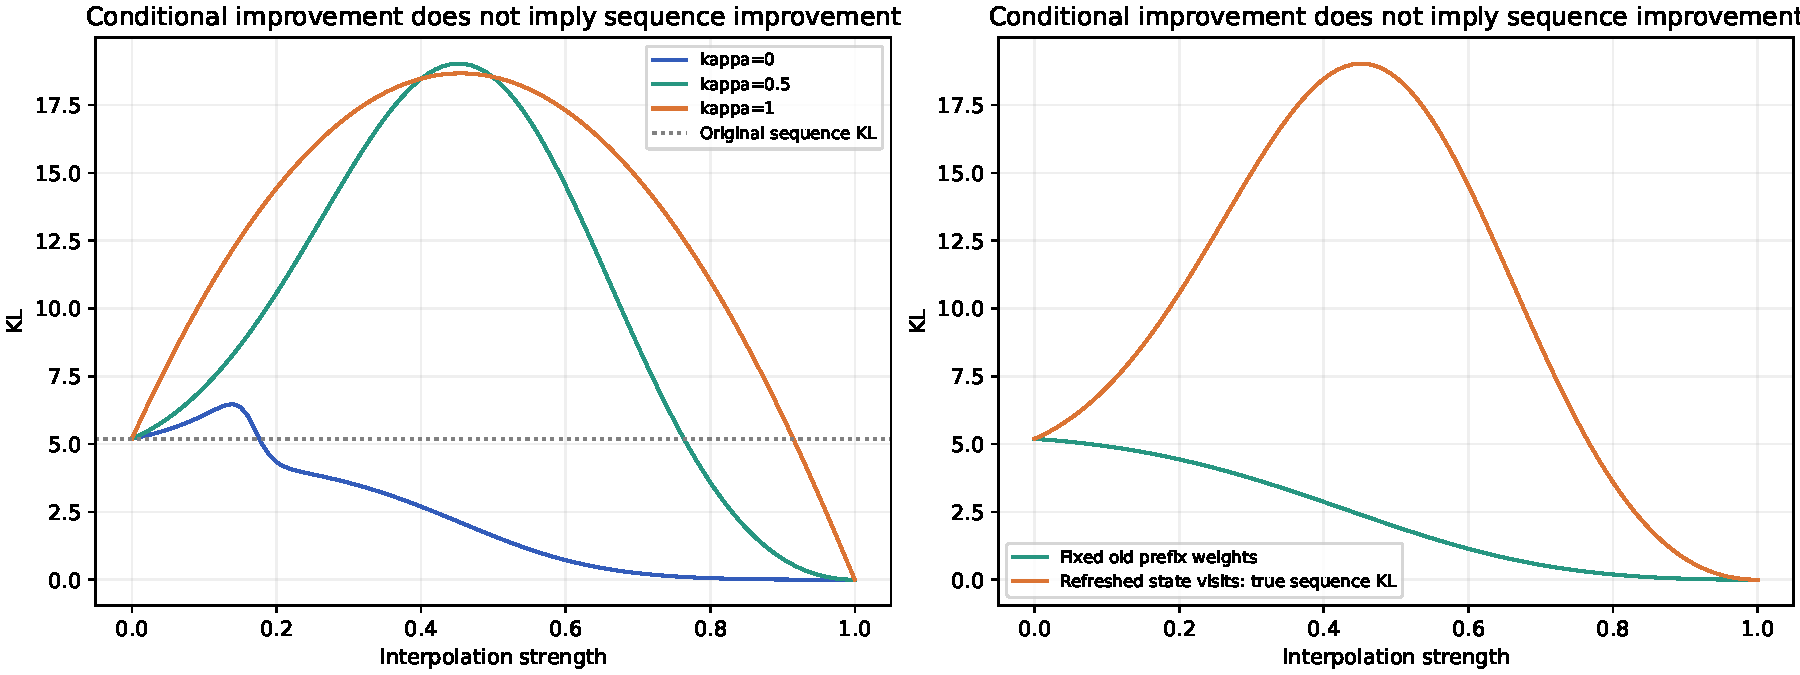
\includegraphics[width=\textwidth]{../../results/power-mean-20261013/sequence-scope-counterexample.pdf}
 \caption{精确条件更新仍可能使完整序列 KL 上升。左图比较三种形状；右图固定平方根形状，对照冻结旧 prefix 权重的条件目标与更新后访问测度下的真实序列 KL。}
 \label{fig:sequence-scope-counterexample}
\end{figure}

\subsection{序列级混合与 Token 级混合的精确差异及后缀价值修正}

同样地，对整条序列分布做混合与逐 Token 做条件混合不能互换：
\begin{enumerate}
\item \textbf{序列算术混合的条件概率包含动态前缀因子}：对序列层面的算术混合 $M=(1-\eta)Q+\eta T$，条件分布为
\begin{equation}
 M(a\mid s)=(1-\eta_s)q(a\mid s)+\eta_st(a\mid s),\qquad
 \eta_s=\frac{\eta T(s)}{(1-\eta)Q(s)+\eta T(s)}.
\end{equation}
它的教师权重 $\eta_s$ 依赖于已经生成的前缀 $s$。固定 $\eta$ 的逐 Token 算术混合因此一般不同于序列层面的算术混合。
\item \textbf{序列几何插值的条件概率包含后缀配分函数}：对序列几何目标 $M(y)\propto Q(y)^{1-\eta}T(y)^\eta$，定义后缀配分函数
\begin{equation}
 Z_\eta(s)=\sum_zQ(z\mid s)^{1-\eta}T(z\mid s)^\eta.
\end{equation}
将带前缀 $s$ 的序列质量先求和再作条件化，得到
\begin{equation}
 M(a\mid s)=q(a\mid s)^{1-\eta}t(a\mid s)^\eta
 \frac{Z_\eta(sa)}{Z_\eta(s)}.
\end{equation}
逐 Token 几何目标忽略了动作相关的后缀配分函数比值 $Z_\eta(sa)/Z_\eta(s)$；它只有在这些后缀因子与动作无关时才恢复完整序列目标。
\item \textbf{真实序列逆向 KL 的一阶方向与后缀价值递推}：记后缀价值函数为 $V^q(s)=\KL(Q(\cdot\mid s)\Vert T(\cdot\mid s))$。链式法则给出动态规划递推：
\begin{equation}
 V^q(s)=\E_{a\sim q(\cdot\mid s)}\left[\log\frac{q(a\mid s)}{t(a\mid s)}+V^q(sa)\right],
\end{equation}
终点处的值为零。对照完整序列 KL 的策略梯度式~\eqref{eq:trajectory-kl-exact-grad} 可知，对某个前缀 $s$ 的局部更新方向，若要精确对齐完整序列逆向 KL，未来成本不能省略，其等效单步负信号为
\begin{equation}
 f_{\mathrm{seq}}^q(s,a)=\log\frac{t(a\mid s)}{q(a\mid s)}-V^q(sa).
\end{equation}
条件中心化后，它给出真实序列逆向 KL 的自然梯度方向。本书主线研究的固定测度 Token 级优化明确保留第一项即时对数概率比，并通过外层同步刷新访问测度 $d_k$ 推进多步蒸馏。
\end{enumerate}

\chapter{归一化商坐标与四种内层投影目标}
\label{ch:four-methods}

第~\ref{ch:foundations} 章证明了固定前缀下 KL 镜像子问题的唯一最优解为 Gibbs 分布 $p_k^{\mathrm G}(a\mid s)\propto q_k(a\mid s)e^{\eta f(s,a)}$。然而，要把这一分布结论转化为参数化神经网络 $\pi_\theta$ 可直接最小化的内层损失函数，必须解决两个核心问题：第一，配分函数对数 $\log Z_f(s)$ 是整个词表上的指数和，如何处理或消去这一归一化常数？第二，不同归一化处理方式（完整配分函数、奖励均值近似、残差中心化、直接变分优化）在总体目标、有限步梯度与最优不动点上究竟有何异同？

本章固定单个前缀 $s$（局部推导中省略条件变量 $s$ 与索引 $k,n$，记 $q$ 为冻结锚点，$p$ 为当前学生，$f$ 为冻结信号），首先建立中心化商空间（quotient space）坐标与概率单纯形之间的精确双射，在同一坐标系下导出 PMD-Part、PMD-Mean、BPO 与 MDPO 四种内层目标的统一几何分解；随后给出四种算法的完整解析梯度、停止梯度策略梯度（PG）形式与更新伪代码；最后深入证明 PMD-Mean 的 Lambert-$W$ 闭式投影、R\'enyi 乘子上下界、大步长 $\eta\to\infty$ 正部加权极限以及超额损失精确分解。

\section{中心化商空间坐标、归一化恢复与四目标分解}
\label{sec:inner-quotient}

对任意严格正概率分布 $\mu\in\Delta_V^\circ$，定义条件中心化算子 $C_\mu h=h-\E_\mu h$。它是将 $\R^V$ 投影到 $\mu$-零均值子空间的幂等线性算子，其核空间恰为常数向量张成的子空间：
\begin{equation}
C_\mu^2=C_\mu,\qquad C_\mu\mathbf1=0,\qquad
\ker C_\mu=\operatorname{span}\{\mathbf1\}.
\end{equation}
商空间视角将相差一个动作无关常数的对数概率比视为同一个等价类代表。概率单纯形的归一化约束 $\sum_a p_a=1$ 唯一确定该常数。

\begin{theorem}[归一化分布与中心化误差向量的一一对应]
\label{thm:quotient-bijection}
给定严格正的 Gibbs 目标分布 $p^{\mathrm G}\in\Delta_V^\circ$ 与锚点 $q\in\Delta_V^\circ$，对任意正学生分布 $p\in\Delta_V^\circ$ 定义中心化对数误差向量与对数配分修正函数：
\begin{equation}
e=C_q\log\frac{p}{p^{\mathrm G}},\qquad
A(e)=\log\E_{p^{\mathrm G}}\bigl[e^{e}\bigr].
\end{equation}
则映射 $p\mapsto e$ 是开单纯形 $\Delta_V^\circ$ 到零均值超平面 $\{e\in\R^V:\E_q e=0\}$ 的光滑双射，其精确逆映射为
\begin{equation}
p_a(e)=p_a^{\mathrm G}\exp\bigl(e_a-A(e)\bigr).
\label{eq:quotient-inverse}
\end{equation}
\end{theorem}
\begin{proof}
令 $h_a=\log(p_a/p_a^{\mathrm G})$，$c=\E_q h$，则 $h=e+c\mathbf1$。利用 $p$ 的概率归一化条件 $\sum_a p_a=1$，有
\begin{align}
1=\sum_a p_a^{\mathrm G}e^{h_a}&=e^c\sum_a p_a^{\mathrm G}e^{e_a},\\
c&=-\log\sum_a p_a^{\mathrm G}e^{e_a}=-A(e).
\end{align}
故任意 $p\in\Delta_V^\circ$ 均满足逆映射式~\eqref{eq:quotient-inverse}。反之，对任意满足 $\E_q e=0$ 的向量 $e$，由式~\eqref{eq:quotient-inverse} 构造的 $p(e)$ 严格为正且总和为 $1$，并满足
\begin{equation}
C_q\log\frac{p(e)}{p^{\mathrm G}}=C_q\bigl(e-A(e)\mathbf1\bigr)=C_q e=e.
\end{equation}
正反复合映射均为恒等映射，双射得证。
\end{proof}

\begin{theorem}[四种内层目标在同一商坐标中的精确表达]
\label{thm:quotient-losses}
设中心化冻结信号为 $G=\eta C_q f$，配分函数为 $Z_f=\E_q[e^{\eta f}]$，并记均值近似遗漏的对数配分修正项为
\begin{equation}
\Delta=\log Z_f-\eta\E_q f
=\log\E_q\bigl[e^G\bigr]=\KL(q\Vert p^{\mathrm G})\ge 0.
\end{equation}
在定理~\ref{thm:quotient-bijection} 的商坐标 $e=C_q\log(p/p^{\mathrm G})$ 下，三种回归残差与四种内层总体目标具有如下精确统一表示：
\begin{align}
R^{\mathrm{Part}}&=e-A(e)\mathbf1,&
R^{\mathrm{BPO}}&=e,&
R^{\mathrm{Mean}}&=e-\bigl(A(e)+\Delta\bigr)\mathbf1,\\
\mathcal L_{\mathrm{Part}}&=\tfrac12\E_q[e^2]+\tfrac12 A(e)^2,\\
\eta\mathcal L_{\mathrm{BPO}}&=\tfrac12\E_q[e^2],\\
\mathcal L_{\mathrm{Mean}}&=\tfrac12\E_q[e^2]+\tfrac12\bigl(A(e)+\Delta\bigr)^2,\\
\mathcal L_{\mathrm{MDPO}}&=\frac1\eta\KL\bigl(p(e)\Vert p^{\mathrm G}\bigr)-\frac1\eta\log Z_f.
\label{eq:quotient-four-losses}
\end{align}
因此，$\log Z_f$ 在 BPO 中被中心化算子消去后，其自由度完全由学生概率分布自身的归一化函数 $A(e)$ 自动恢复。PMD-Part 与 BPO 共享唯一的零误差最优分布 $e=0$（即 $p=p^{\mathrm G}$），但具有不同的非零误差目标函数；PMD-Mean 则因附加项 $(A(e)+\Delta)^2$ 而在 $\Delta>0$ 时偏移了全局最优点。
\end{theorem}
\begin{proof}
由 Gibbs 分布定义~\eqref{eq:ch2-optimal-policy} 可知 $\log(p^{\mathrm G}/q)=\eta f-\log Z_f=G-\Delta\mathbf1$。将其与双射展开式 $\log(p/p^{\mathrm G})=e-A(e)\mathbf1$ 相加，得到学生对锚点的对数比率：
\begin{equation}
U=\log\frac pq=G-\Delta\mathbf1+e-A(e)\mathbf1.
\end{equation}
代入残差定义，立得 $R^{\mathrm{Part}}=U-\eta f+\log Z_f=U-G+\Delta\mathbf1=e-A(e)\mathbf1$，以及 $R^{\mathrm{Mean}}=U-G=e-(A(e)+\Delta)\mathbf1$。对完整残差应用 $C_q$，由于 $\E_q e=0$，有
\begin{equation}
R^{\mathrm{BPO}}=C_q R^{\mathrm{Part}}=C_q\bigl(e-A(e)\mathbf1\bigr)=e.
\end{equation}
在锚点测度 $q$ 下对残差平方求期望，利用交叉项 $\E_q[e]=0$，正交分解给出
\begin{align}
\E_q\bigl[(e-A(e))^2\bigr]&=\E_q[e^2]-2A(e)\E_q[e]+A(e)^2=\E_q[e^2]+A(e)^2,\\
\E_q\bigl[(e-A(e)-\Delta)^2\bigr]&=\E_q[e^2]+\bigl(A(e)+\Delta\bigr)^2.
\end{align}
MDPO 的表达式直接来自定理~\ref{thm:ch2-gibbs} 的变分恒等式~\eqref{eq:ch2-kl-decomp}。最后，对 $U$ 求锚点期望可得
\begin{equation}
\E_q[U]=-\Delta-A(e),\qquad K_{qp}=\KL(q\Vert p)=-\E_q[U]=\Delta+A(e)\ge0.
\end{equation}
这同时表明 $A(e)=K_{qp}-\Delta\ge -\Delta$。注意 $A(e)=\log\E_{p^{\mathrm G}}[e^e]$ 的指数期望在 $p^{\mathrm G}$ 下计算，而 $e$ 的零均值中心化在 $q$ 下定义，二者测度不同，不可混用。
\end{proof}

利用 $K_{qp}=\Delta+A(e)$，我们还可以将式~\eqref{eq:quotient-four-losses} 改写为以 BPO 为基准的正交分解式：
\begin{align}
\mathcal L_{\mathrm{Part}}&=\eta\mathcal L_{\mathrm{BPO}}
+\frac12\bigl[\Delta-\KL(q\Vert p)\bigr]^2,\\
\mathcal L_{\mathrm{Mean}}&=\eta\mathcal L_{\mathrm{BPO}}
+\frac12\KL(q\Vert p)^2.
\label{eq:quotient-penalties}
\end{align}
式~\eqref{eq:quotient-penalties} 清晰地揭示了三种回归目标的本质区别：PMD-Part 在 BPO 的基础上惩罚“当前学生步幅 $\KL(q\Vert p)$ 与理想 Gibbs 步幅 $\Delta=\KL(q\Vert p^{\mathrm G})$ 之间的标量偏差”；而 PMD-Mean 则在 BPO 的基础上额外施加了惩罚项 $\frac12\KL(q\Vert p)^2$，从而将充分优化后的学生分布向锚点 $q$ 拉近。

\begin{proposition}[成对动作差分回归完全消去双侧归一化常数]
\label{prop:quotient-pairwise}
令未中心化差分为 $h_a=U_a-\eta f_a$，并设两个动作 $a,b\overset{\mathrm{iid}}{\sim}q$ 独立同分布采样自锚点。则 BPO 损失可等价表示为成对平方差期望：
\begin{equation}
\mathcal L_{\mathrm{BPO}}=
\frac1{4\eta}\E_{a,b\sim q}\bigl[(h_a-h_b)^2\bigr].
\end{equation}
若学生分布由无约束 Logits $z$ 通过 $p=\operatorname{softmax}(z)$ 参数化，则成对差分进一步简化为
\begin{equation}
h_a-h_b=(z_a-z_b)-(\log q_a-\log q_b)-\eta(f_a-f_b).
\end{equation}
\end{proposition}
\begin{proof}
由 $a,b\sim q$ 的独立同分布性质，$\E_{a,b}[h_a h_b]=(\E_q h)^2$，故
\begin{equation}
\E_{a,b}\bigl[(h_a-h_b)^2\bigr]=2\E_q[h^2]-2(\E_q h)^2=2\Var_q(h)=2\E_q\bigl[(R^{\mathrm{BPO}})^2\bigr]=4\eta\mathcal L_{\mathrm{BPO}}.
\end{equation}
将 $\log p_a=z_a-\log\sum_v e^{z_v}$ 代入 $U_a-U_b=\log p_a-\log p_b-(\log q_a-\log q_b)$，学生自身的对数配分函数 $\log\sum_v e^{z_v}$ 在差分中也精确相消。因此，成对回归无需把 Gibbs 配分函数 $\log Z_f$ 或学生配分函数作为显式数值输入。
\end{proof}

\section{从镜像最优性方程到四种内层更新算法}
\label{sec:ch2-objective-derivation}
\label{sec:ch2-four-methods}

定理~\ref{thm:ch2-gibbs} 的最优性方程 $\log(p_k^{\mathrm G}(a\mid s)/q_k(a\mid s))=\eta f(s,a)-\log Z_f(s)$ 给出了一条逐 Token 恒等式：
\begin{equation}
\label{eq:ch2-logratio-equation}
\log\frac{ p_k^{\mathrm G}(a\mid s)}{ q_k(a\mid s)}
=\eta f(s,a)-\log Z_f(s).
\end{equation}
定义完整镜像方程残差
\begin{equation}
R_{k,n}^{\mathrm{Part}}(s,a)
\coloneqq
\log\frac{ p_{k,n}(a\mid s)}{ q_k(a\mid s)}
-\eta f(s,a)+\log Z_f(s).
\label{eq:ch2-mirror-equation-residual}
\end{equation}
在参数化内层训练中，我们选择锚点诱导的乘积测度 $L_2(d_k q_k)$ 作为平方回归的投影几何，以便与冻结采样轨迹的经验测度直接对齐：
\begin{equation}
\lVert R_{k,n}^{\mathrm{Part}}\rVert_k^2
\coloneqq
\mathbb E_{s\sim d_k}\mathbb E_{a\sim q_k(\cdot\mid s)}
\left[R_{k,n}^{\mathrm{Part}}(s,a)^2\right].
\label{eq:ch2-anchor-projection-norm}
\end{equation}
若实际采样动作来自另一个行为策略 $\beta_k$（且 $q_k\ll\beta_k$），则必须乘以冻结的重要性权重 $q_k(a\mid s)/\beta_k(a\mid s)$，否则优化的将是 $L_2(d_k\beta_k)$ 投影。

\begin{proposition}[平方回归的函数类投影含义]
\label{prop:ch2-regression-projection}
当参数化学生模型族不能精确表示镜像最优对数比率~\eqref{eq:ch2-logratio-equation} 时，PMD-Part 的精确内层解是镜像最优性方程在模型族诱导的 $L_2(d_k q_k)$ 几何下的最佳平方逼近投影；若前缀访问测度改为 $\nu$，投影几何相应变为 $L_2(\nu q_k)$。在任意光滑可行参数曲线的一阶切向扰动 $v$ 上，局部最优残差 $\mathscr E^\star$ 满足正交性必要条件 $\mathbb E_{\nu, q_k}[\mathscr E^\star v]=0$。
\end{proposition}
\begin{proof}
对光滑参数曲线 $\theta(u)$ 下的平方损失 $\frac12\mathbb E_{\nu,q_k}[\mathscr E_{\theta(u)}^2]$ 在局部极值点 $u=0$ 处求导，由一阶驻点条件 $\frac{d}{du}\big|_{u=0}=0$ 直接得到 $\mathbb E_{\nu,q_k}[\mathscr E^\star v]=0$，其中 $v=\frac{d}{du}U_{\theta(u)}\big|_{u=0}$ 为可行切空间方向。由于非线性神经网络诱导的对数比率流形通常非凸，该正交条件是局部最优的必要条件；仅当目标属于可行集且测度完整覆盖时，全局最小残差才恒为零。
\end{proof}

下面依次给出 PMD-Part、PMD-Mean、BPO 与 MDPO 四种内层方法的总体损失、解析梯度、停止梯度 PG 形式与标准更新伪代码。所有 PG 表达式均在 $\theta=\theta_{k,n}$ 处计算，括号内的标量系数整体施加停止梯度算子 $\sg(\cdot)$，仅由最右侧的 $\nabla_\theta\log p_{k,n}(a\mid s)$ 接收反向传播梯度。

\subsection{PMD-Part：回归完整 Gibbs 对数概率比}
\label{subsec:ch2-pmd-loss-derivation}
\label{sec:ch2-pmd-part}

PMD-Part 直接最小化完整镜像残差~\eqref{eq:ch2-mirror-equation-residual} 的锚点加权平方期望：
\begin{equation}
\label{eq:ch2-regression-from-mirror,eq:ch2-part-loss}
\mathcal L_{\mathrm{Part}}(\theta)
=\frac12\mathbb E_{s\sim d_k,\,a\sim q_k}
\left[
\log\frac{ p_{k,n}(a\mid s)}{ q_k(a\mid s)}
-\eta f(s,a)+\sg\!\left(\log Z_f(s)\right)
\right]^2.
\end{equation}
固定前缀 $s$ 后，由于 $q_k$、$f$ 与 $Z_f$ 在本轮内层全部冻结，且 $\nabla_\theta U_{k,n}(s,a)=\nabla_\theta\log p_{k,n}(a\mid s)=\psi_{k,n}(s,a)$，直接求导可得解析梯度与采样 PG 形式：
\begin{align}
\nabla_\theta\mathcal L_{\mathrm{Part}}(s)
&=\sum_{a\in\mathcal V} q_k(a\mid s)R_{k,n}^{\mathrm{Part}}(s,a)\psi_{k,n}(s,a)\nonumber\\
&=\mathbb E_{a\sim q_k(\cdot\mid s)}\left[
\sg\!\left(
\log\frac{ p_{k,n}(a\mid s)}{ q_k(a\mid s)}
-\eta f(s,a)+\log Z_f(s)
\right)\nabla_\theta\log p_{k,n}(a\mid s)\right].
\label{eq:ch2-part-gradient-bridge,eq:ch2-part-gradient,eq:ch2-part-pg}
\end{align}
在标准 OPD 中代入 $f=r_k=\log(t/q_k)$，其单样本 PG 更新项即为
\begin{equation}
\label{eq:ch2-part-opd-pg}
\sg\!\left[
\begin{aligned}
&U_{k,n}(s,a)-\eta\bigl(\log t(a\mid s)-\log q_k(a\mid s)\bigr)\\
&\quad+\log\mathbb E_{v\sim q_k}\exp\!\left(\eta[\log t(v\mid s)-\log q_k(v\mid s)]\right)
\end{aligned}
\right]\nabla_\theta\log p_{k,n}(a\mid s).
\end{equation}

\begin{algorithm}[ht]
\caption{PMD-Part 内层更新\\{\small\textit{数学语义：固定锚点测度下的完整 Gibbs 对数概率比平方回归}}}
\begin{algorithmic}[1]
\Require 冻结锚点 $q_k$，教师信号 $f$，前缀批次 $\{s_i\}_{i=1}^B$，镜像步长 $\eta$，内层学习率 $\alpha_{k,n}$
\Ensure 更新后的学生参数 $\theta_{k,n+1}$
\For{$i=1,\ldots,B$}
    \State 从锚点采样动作 $a_i\sim q_k(\cdot\mid s_i)$
    \State $\log Z_i\gets\operatorname{logsumexp}_{v\in\mathcal V}\bigl(\log q_k(v\mid s_i)+\eta f(s_i,v)\bigr)$
    \State $H_i\gets\eta f(s_i,a_i)-\sg(\log Z_i)$
    \State $U_i\gets\log p_{k,n}(a_i\mid s_i)-\sg(\log q_k(a_i\mid s_i))$
    \State $\ell_i\gets\frac12\bigl(U_i-\sg(H_i)\bigr)^2$
\EndFor
\State $g_{k,n}\gets\nabla_\theta\bigl(B^{-1}\sum_{i=1}^B\ell_i\bigr)$
\State $\theta_{k,n+1}\gets\theta_{k,n}-\alpha_{k,n}g_{k,n}$
\State \Return $\theta_{k,n+1}$
\end{algorithmic}
\end{algorithm}

\subsection{PMD-Mean：中心化奖励回归与留一法（LOO）实现}
\label{sec:ch2-pmd-mean}

PMD-Mean 将完整目标中的 $\log Z_f(s)$ 替换为线性均值 $\eta\bar f_k(s)$，即仅对冻结奖励信号做中心化（$G_k=\eta(f-\bar f_k)$），而不对学生对数比率 $U_{k,n}$ 做条件中心化：
\begin{equation}
\mathcal L_{\mathrm{Mean}}(\theta)
=\frac12\mathbb E_{s\sim d_k,\, a\sim q_k}
\left[\log\frac{ p_{k,n}(a\mid s)}{ q_k(a\mid s)}
-\eta\bigl(f(s,a)-\bar f_k(s)\bigr)\right]^2.
\label{eq:ch2-mean-loss-bridge}
\end{equation}
由于奖励中心 $\bar f_k(s)$ 在整个内层循环中完全冻结，直接对 $\theta$ 求导得到解析梯度与采样 PG 形式：
\begin{align}
\nabla_\theta\mathcal L_{\mathrm{Mean}}(s)
&=\mathbb E_{a\sim q_k(\cdot\mid s)}
\left[\bigl(U_{k,n}(s,a)-G_k(s,a)\bigr)\psi_{k,n}(s,a)\right]\nonumber\\
&=\mathbb E_{a\sim q_k(\cdot\mid s)}\left[
\sg\!\left(U_{k,n}(s,a)-\eta\bigl(f(s,a)-\bar f_k(s)\bigr)\right)
\nabla_\theta\log p_{k,n}(a\mid s)\right].
\label{eq:ch2-mean-gradient-bridge,eq:ch2-mean-pg}
\end{align}
在标准 OPD 中，$\bar f_k(s)=\mathbb E_{v\sim q_k}[r_k(s,v)]=-K_{qt,k}(s)$，故单样本 PG 项为
\begin{equation}
\label{eq:ch2-mean-opd-pg}
\sg\!\left[
U_{k,n}(s,a)-\eta\bigl(\log t(a\mid s)-\log q_k(a\mid s)
+K_{qt,k}(s)\bigr)
\right]\nabla_\theta\log p_{k,n}(a\mid s).
\end{equation}
在仅能采样动作的无完整词表场景下，若同一前缀 $s_i$ 抽取了 $m\ge 2$ 个独立锚点动作 $\{a_{ij}\}_{j=1}^m$，可使用留一法（Leave-One-Out, LOO）均值估计冻结奖励中心：
\begin{equation*}
\widehat{\bar f}_{-j}(s_i)=\frac1{m-1}\sum_{\ell\ne j}f(s_i,a_{i\ell}).
\end{equation*}
由于 $\widehat{\bar f}_{-j}$ 不依赖学生参数且与当前动作 $a_{ij}$ 条件独立，LOO 平方损失的随机梯度对总体 Mean 梯度严格无偏（其精确期望损失见后文命题~\ref{dyn:prop:mean-opd-loo-expectation}）。

\begin{algorithm}[ht]
\caption{PMD-Mean 内层更新\\{\small\textit{数学语义：中心化奖励目标在概率归一化约束集上的投影}}}
\begin{algorithmic}[1]
\Require 冻结锚点 $q_k$，信号 $f$，前缀批次 $\{s_i\}_{i=1}^{B}$，同前缀样本数 $m\ge2$，步长 $\eta$，学习率 $\alpha_{k,n}$
\Ensure 更新后的学生参数 $\theta_{k,n+1}$
\For{每个前缀 $s_i$ ($i=1,\ldots,B$)}
    \For{$j=1,\ldots,m$}
        \State 采样独立动作 $a_{ij}\sim q_k(\cdot\mid s_i)$
        \State $U_{ij}\gets\log p_{k,n}(a_{ij}\mid s_i)-\sg(\log q_k(a_{ij}\mid s_i))$
        \State $F_{ij}\gets f(s_i,a_{ij})$
    \EndFor
    \For{$j=1,\ldots,m$}
        \State $\bar F_{-j}\gets(m-1)^{-1}\sum_{\ell\ne j}F_{i\ell}$
        \State $\ell_{ij}\gets\frac12\bigl[U_{ij}-\eta\sg(F_{ij}-\bar F_{-j})\bigr]^2$
    \EndFor
\EndFor
\State $g_{k,n}\gets\nabla_\theta\bigl[(Bm)^{-1}\sum_{i,j}\ell_{ij}\bigr]$
\State $\theta_{k,n+1}\gets\theta_{k,n}-\alpha_{k,n}g_{k,n}$
\State \Return $\theta_{k,n+1}$
\end{algorithmic}
\end{algorithm}

\subsection{BPO：中心化完整最优性残差}
\label{subsec:ch2-bpo-loss-derivation}
\label{sec:ch2-bpo}

BPO 对完整的“学生对数比率减缩放信号”按冻结锚点 $q_k$ 做条件中心化，从而将动作无关的配分函数对数 $\log Z_f(s)$ 精确消去：
\begin{align}
R_{k,n}^{\mathrm{BPO}}(s,a)
&\coloneqq U_{k,n}(s,a)-\eta f(s,a)
-\mathbb E_{ q_k}\bigl[U_{k,n}(s,\cdot)-\eta f(s,\cdot)\mid s\bigr]
\label{eq:ch2-bpo-from-optimality}\\
&=U_{k,n}(s,a)-G_k(s,a)+K_{qp,k,n}(s).
\label{eq:ch2-bpo-expanded,eq:ch2-bpo-residual}
\end{align}
这里利用了 $\mathbb E_{q_k}[U_{k,n}\mid s]=-K_{qp,k,n}(s)$，故学生条件 KL 项前为正号。在 OPD 实例化 $f=r_k$ 下，残差展开为
\begin{equation}
R_{k,n}^{\mathrm{BPO}}(s,a)
=\log\frac{ p_{k,n}(a\mid s)}{ q_k(a\mid s)}+K_{qp,k,n}(s)
-\eta\left(\log\frac{ t(a\mid s)}{ q_k(a\mid s)}+K_{qt,k}(s)\right).
\label{eq:ch2-bpo-opd-expanded}
\end{equation}
BPO 最小化带 $1/(2\eta)$ 缩放的平方残差损失：
\begin{equation}
\mathcal L_{\mathrm{BPO}}(\theta)
=\frac1{2\eta}\mathbb E_{s\sim d_k,\, a\sim q_k}\bigl[(R_{k,n}^{\mathrm{BPO}}(s,a))^2\bigr].
\label{eq:ch2-bpo-loss-bridge}
\end{equation}
由于学生中心 $K_{qp,k,n}(s)$ 依赖于当前参数 $\theta$，其导数为 $\nabla_\theta K_{qp,k,n}(s)=-\bar\psi_{k,n}(s)$，因此 $\nabla_\theta R_{k,n}^{\mathrm{BPO}}=\psi_{k,n}-\bar\psi_{k,n}$。对式~\eqref{eq:ch2-bpo-loss-bridge} 求导并利用条件零均值恒等式 $\mathbb E_{q_k}[R_{k,n}^{\mathrm{BPO}}\mid s]=0$，中心导数交叉项 $\mathbb E_{q_k}[R_{k,n}^{\mathrm{BPO}}\mid s]\bar\psi_{k,n}$ 精确归零：
\begin{align}
\nabla_\theta\mathcal L_{\mathrm{BPO}}(s)
&=\frac1\eta\mathbb E_{q_k}\bigl[R_{k,n}^{\mathrm{BPO}}(\psi_{k,n}-\bar\psi_{k,n})\mid s\bigr]
\label{eq:ch2-bpo-gradient-bridge,eq:ch2-bpo-gradient}\\
&=\mathbb E_{a\sim q_k(\cdot\mid s)}\left[
\sg\!\left(\frac{U_{k,n}(s,a)+K_{qp,k,n}(s)}\eta-f(s,a)+\bar f_k(s)\right)\nabla_\theta\log p_{k,n}(a\mid s)\right].
\label{eq:ch2-bpo-pg}
\end{align}
在 OPD 设定下，其单样本 PG 表达式为
\begin{equation}
\label{eq:ch2-bpo-opd-pg}
\sg\!\left[
\frac{U_{k,n}(s,a)+K_{qp,k,n}(s)}{\eta}
-\bigl(\log t(a\mid s)-\log q_k(a\mid s)\bigr)
-K_{qt,k}(s)
\right]\nabla_\theta\log p_{k,n}(a\mid s).
\end{equation}

\paragraph{注记（有限样本中心导数协方差与无偏修正系数）。}
在总体期望中，$\bar\psi_{k,n}$ 项的消失依赖于精确条件零均值 $\mathbb E_{q_k}[R^{\mathrm{BPO}}\mid s]=0$。若在有限样本下直接对经验平方损失求自动微分（保留学生中心导数）：设用 $1$ 个主动作 $a_i\sim q_k$ 和 $m$ 个独立辅助动作 $b_{i1},\ldots,b_{im}\sim q_k$ 估计中心，令 $h(s,a)=U_{k,n}(s,a)-\eta f(s,a)$，则
\begin{equation*}
\mathbb E\left[\left(h(s,a_i)-\frac1m\sum_{\ell=1}^m h(s,b_{i\ell})\right)^2\right]
=\left(1+\frac1m\right)\operatorname{Var}_{ q_k}(h\mid s).
\end{equation*}
因此经验平方损失必须乘以修正因子 $\frac{m}{m+1}$（若对同前缀共 $m\ge 2$ 个动作采用留一法中心，则修正因子为 $\frac{m-1}{m}$），其自动微分梯度才对总体 BPO 梯度严格无偏。

\begin{algorithm}[ht]
\caption{BPO 内层更新\\{\small\textit{数学语义：固定锚点下对中心化完整残差求平方损失}}}
\begin{algorithmic}[1]
\Require 冻结锚点 $q_k$，信号 $f$，前缀批次 $\{s_i\}_{i=1}^{B}$，辅助动作数 $m\ge1$，步长 $\eta$，学习率 $\alpha_{k,n}$
\Ensure 更新后的学生参数 $\theta_{k,n+1}$
\For{每个前缀 $s_i$ ($i=1,\ldots,B$)}
    \State 独立采样主动作 $a_i\sim q_k(\cdot\mid s_i)$ 与辅助动作 $b_{i1},\ldots,b_{im}\sim q_k(\cdot\mid s_i)$
    \State $h_i\gets U_{k,n}(s_i,a_i)-\eta f(s_i,a_i)$
    \State $\bar h_i\gets m^{-1}\sum_{\ell=1}^{m}\bigl[U_{k,n}(s_i,b_{i\ell})-\eta f(s_i,b_{i\ell})\bigr]$
    \State $\widehat R_i^{\mathrm{BPO}}\gets h_i-\bar h_i$, \quad $\ell_i\gets\frac{m}{m+1}\frac{(\widehat R_i^{\mathrm{BPO}})^2}{2\eta}$
\EndFor
\State $g_{k,n}\gets\nabla_\theta\bigl(B^{-1}\sum_{i=1}^B\ell_i\bigr)$
\State $\theta_{k,n+1}\gets\theta_{k,n}-\alpha_{k,n}g_{k,n}$
\State \Return $\theta_{k,n+1}$
\end{algorithmic}
\end{algorithm}

\subsection{MDPO：直接最小化负镜像变分目标}
\label{subsec:ch2-mdpo-loss-derivation}
\label{sec:ch2-mdpo-generic}

MDPO（Mirror Descent Policy Optimization）直接将原始镜像泛函~\eqref{eq:ch2-mirror} 取负作为最小化损失：
\begin{align}
\mathcal L_{\mathrm{MDPO}}(\theta)
&=-\mathbb E_{s\sim d_k,\,a\sim p_{k,n}}[f(s,a)]
+\frac1\eta\mathbb E_{s\sim d_k}\operatorname{KL}\bigl( p_{k,n}(\cdot\mid s)\Vert q_k(\cdot\mid s)\bigr)
\label{eq:ch2-mdpo-objective-bridge}\\
&=\mathbb E_{s\sim d_k}\left[-\frac1\eta\log Z_f(s)
+\frac1\eta\operatorname{KL}\bigl( p_{k,n}(\cdot\mid s)\Vert p_k^{\mathrm G}(\cdot\mid s)\bigr)\right].
\label{eq:ch2-mdpo-kl-gap}
\end{align}
注意此处 KL 的第一自变量是当前学生 $p_{k,n}$，与 BPO 学生中心 $K_{qp,k,n}=\KL(q_k\Vert p_{k,n})$ 的方向相反。完整词表下 $\KL(p_{k,n}\Vert q_k)$ 由下式精确求和：
\begin{equation}
\operatorname{KL}( p_{k,n}\Vert q_k)
=\sum_{a\in\mathcal V} p_{k,n}(a\mid s)U_{k,n}(s,a).
\label{eq:ch2-mdpo-full-kl}
\end{equation}
当动作采样自冻结锚点 $q_k$ 时，引入重要性比率 $\omega_{k,n}=p_{k,n}/q_k=e^{U_{k,n}}$，单前缀损失可写为
\begin{equation}
\mathcal L_{\mathrm{MDPO}}(s)
=\mathbb E_{a\sim q_k}\left[e^{U_{k,n}}\left(\frac{U_{k,n}}\eta-f\right)\;\middle|\; s\right].
\label{eq:ch2-mdpo-sample-integrand}
\end{equation}
对学生采样测度与对数比率同时求导，并利用学生测度下的零均值恒等式 $\mathbb E_{p_{k,n}}[\psi_{k,n}\mid s]=0$ 消去常数 $1/\eta$ 项，得到解析梯度与采样 PG 形式：
\begin{align}
\nabla_\theta\mathcal L_{\mathrm{MDPO}}(s)
&=\mathbb E_{a\sim p_{k,n}}\left[\left(\frac{U_{k,n}+1}\eta-f\right)\psi_{k,n}\;\middle|\; s\right]
=\mathbb E_{a\sim p_{k,n}}\left[\sg\!\left(\frac{U_{k,n}}\eta-f\right)\psi_{k,n}\;\middle|\; s\right]
\label{eq:ch2-mdpo-gradient-bridge}\\
&=\mathbb E_{a\sim q_k(\cdot\mid s)}\left[
\sg\!\left(
\frac{ p_{k,n}(a\mid s)}{ q_k(a\mid s)}
\left[\frac1\eta\log\frac{ p_{k,n}(a\mid s)}{ q_k(a\mid s)}-f(s,a)\right]
\right)\nabla_\theta\log p_{k,n}(a\mid s)\right].
\label{eq:ch2-mdpo-generic-gradient,eq:ch2-mdpo-pg}
\end{align}
代入 OPD 信号 $f=r_k=\log(t/q_k)$，单样本 PG 更新项即为
\begin{equation}
\label{eq:ch2-mdpo-opd-pg}
\sg\!\left[
\frac{ p_{k,n}(a\mid s)}{ q_k(a\mid s)}
\left(\frac1\eta\log\frac{ p_{k,n}(a\mid s)}{ q_k(a\mid s)}
-\log\frac{ t(a\mid s)}{ q_k(a\mid s)}\right)
\right]\nabla_\theta\log p_{k,n}(a\mid s).
\end{equation}
若配合自然梯度（Natural Gradient）更新，设 Fisher 信息矩阵为 $F_{k,n}=\mathbb E_{d_k, p_{k,n}}[\psi_{k,n}\psi_{k,n}^\top]$（锚点采样下通过 $\sg(\omega_{k,n})$ 校正测度），则使用伪逆或阻尼逆 $(F_{k,n}+\gamma I)^\dagger$ 预条件梯度，如下列算法所示。

\begin{algorithm}[ht]
\caption{MDPO 自然梯度内层更新\\{\small\textit{数学语义：最小化固定前缀测度下的负镜像变分目标}}}
\begin{algorithmic}[1]
\Require 冻结锚点 $q_k$，信号 $f$，前缀批次 $\{s_i\}_{i=1}^{B}$，步长 $\eta$，自然步长 $\alpha_{k,n}$，阻尼 $\gamma\ge0$
\Ensure 更新后的学生参数 $\theta_{k,n+1}$
\For{每个前缀 $s_i$ ($i=1,\ldots,B$)}
    \State 采样动作 $a_i\sim q_k(\cdot\mid s_i)$
    \State $U_i\gets U_{k,n}(s_i,a_i)$,\quad $w_i\gets e^{U_i}$
    \State $\ell_i\gets w_i\bigl(U_i/\eta-f(s_i,a_i)\bigr)$ \Comment{保留指数权重 $w_i$ 对学生参数的导数}
    \State $g_i^{\mathrm{score}}\gets\nabla_\theta\log p_{k,n}(a_i\mid s_i)$
\EndFor
\State $g_{k,n}\gets\nabla_\theta\bigl(B^{-1}\sum_{i=1}^B\ell_i\bigr)$
\State $F\gets B^{-1}\sum_{i=1}^B\sg(w_i)g_i^{\mathrm{score}}(g_i^{\mathrm{score}})^\top$
\State $\theta_{k,n+1}\gets\theta_{k,n}-\alpha_{k,n}(F+\gamma I)^\dagger g_{k,n}$
\State \Return $\theta_{k,n+1}$
\end{algorithmic}
\end{algorithm}

\subsection{四种内层目标的共同根定理与梯度差恒等式}

\begin{theorem}[三种方法的共同 Gibbs 解与 PMD-Mean 的分离]
\label{thm:ch2-inner-common-root}
在独立表格策略（tabular policy）、完整动作支持集（$q_k>0$）和精确词表期望下，PMD-Part、BPO 与 MDPO 的唯一总体全局最优解均为式~\eqref{eq:ch2-optimal-policy} 的 Gibbs 分布 $p_k^{\mathrm G}$：
\begin{equation}
\label{eq:ch2-four-methods-common-gibbs}
 p_{k,n}^{\star}(a\mid s)
=\frac{ q_k(a\mid s)e^{\eta f(s,a)}}{\mathbb E_{v\sim q_k(\cdot\mid s)}e^{\eta f(s,v)}}.
\end{equation}
PMD-Mean 的唯一总体全局最优解则是定理~\ref{thm:ch2-mean-lambert} 给出的 Lambert-$W$ 分布 $p_k^{\mathrm M}$；只要冻结信号 $f(s,\cdot)$ 在该前缀上非恒定，就有 $p_k^{\mathrm M}\ne p_k^{\mathrm G}$。
\end{theorem}
\begin{proof}
由定理~\ref{thm:quotient-losses} 的商坐标分解式~\eqref{eq:quotient-four-losses}，PMD-Part、BPO 与 MDPO 的最小损失均当且仅当中心化误差 $e=0$（从而 $A(e)=0$）时达到，对应唯一分布 $p(0)=p_k^{\mathrm G}$。PMD-Mean 的唯一受约束全局最小点及其与 Gibbs 解的严格分离由下一节定理~\ref{thm:ch2-mean-lambert} 给出。
\end{proof}

\begin{proposition}[PMD-Mean 与 BPO 的损失及梯度精确差异]
\label{prop:ch2-mean-bpo-gap}
固定前缀 $s$，Mean 与 BPO 的残差满足 $R_{k,n}^{\mathrm{Mean}}=R_{k,n}^{\mathrm{BPO}}-K_{qp,k,n}(s)$，因此两者的总体损失与参数梯度恒满足
\begin{align}
\mathcal L_{\mathrm{Mean}}(s)&=\eta\mathcal L_{\mathrm{BPO}}(s)+\frac12\bigl(K_{qp,k,n}(s)\bigr)^2,\\
\nabla_\theta\mathcal L_{\mathrm{Mean}}(s)&=\eta\nabla_\theta\mathcal L_{\mathrm{BPO}}(s)+K_{qp,k,n}(s)\nabla_\theta K_{qp,k,n}(s).
\label{eq:ch2-mean-bpo-gap}
\end{align}
\end{proposition}
\begin{proof}
利用 $\mathbb E_{ q_k}[R_{k,n}^{\mathrm{BPO}}\mid s]=0$ 展开平方期望即得第一式，两边对 $\theta$ 求导即得第二式。注意到 $\nabla_\theta K_{qp,k,n}=-\bar\psi_{k,n}$，故两者的负梯度（下降方向）满足
\begin{equation*}
-\nabla_\theta\mathcal L_{\mathrm{Mean}}
=-\eta\nabla_\theta\mathcal L_{\mathrm{BPO}}+K_{qp,k,n}\bar\psi_{k,n}.
\end{equation*}
在内层起点 $p_{k,0}=q_k$ 处，$K_{qp,k,0}=0$ 且 $\bar\psi_{k,0}=0$，两者具有完全相同的同尺度下降方向；一旦 $p_{k,n}$ 离开锚点 $q_k$（例如在独立 Softmax Logits 下 $\bar\psi_{k,n}=q_k-p_{k,n}$），Mean 会比同尺度 BPO 多出一个将学生拉回锚点的恢复力 $K_{qp,k,n}(q_k-p_{k,n})$。
\end{proof}

\begin{proposition}[BPO 与 PMD-Part 的梯度精确差异]
\label{prop:ch2-bpo-part-gradient-gap}
固定前缀 $s$，定义标量差值函数
\begin{equation}
C_{k,n}(s)\coloneqq\log Z_f(s)-\eta\bar f_k(s)-K_{qp,k,n}(s)=\Delta(s)-K_{qp,k,n}(s).
\label{eq:ch2-bpo-part-qc}
\end{equation}
则 $R_{k,n}^{\mathrm{BPO}}=R_{k,n}^{\mathrm{Part}}-C_{k,n}(s)$，且两者的总体参数梯度满足
\begin{equation}
\nabla_\theta\mathcal L_{\mathrm{BPO}}(s)
=\frac1\eta\nabla_\theta\mathcal L_{\mathrm{Part}}(s)
-\frac{C_{k,n}(s)}\eta\bar\psi_{k,n}(s).
\label{eq:ch2-bpo-part-gradient-gap}
\end{equation}
\end{proposition}
\begin{proof}
由残差定义直接相减可得 $R_{k,n}^{\mathrm{Part}}-R_{k,n}^{\mathrm{BPO}}=\log Z_f-\eta\bar f_k-K_{qp,k,n}=C_{k,n}$。代入 BPO 梯度式并利用 $\mathbb E_{q_k}[R_{k,n}^{\mathrm{BPO}}\mid s]=0$：
\begin{align*}
\nabla_\theta\mathcal L_{\mathrm{BPO}}(s)
&=\frac1\eta\mathbb E_{ q_k}\bigl[(R_{k,n}^{\mathrm{Part}}-C_{k,n})\psi_{k,n}\mid s\bigr]
=\frac1\eta\nabla_\theta\mathcal L_{\mathrm{Part}}(s)-\frac{C_{k,n}}\eta\bar\psi_{k,n}.
\end{align*}
在 Gibbs 解 $p=p_k^{\mathrm G}$ 处，$K_{qp,k,n}=\Delta$，故 $C_{k,n}=0$，两梯度同时归零；在一般参数点处，仅当 $C_{k,n}\bar\psi_{k,n}=0$（如内层起点 $p=q_k$ 使得 $\bar\psi=0$）时两者同向。
\end{proof}

\section{PMD-Mean 的 Lambert-\texorpdfstring{$W$}{W} 投影理论与精细误差结构}
\label{dyn:mean-static}

本节深入分析 PMD-Mean 在概率归一化约束下的精确单轮行为。固定前缀 $s$，记
\begin{align}
 q_a&=q_k(a\mid s), & t_a&=t(a\mid s),\notag\\
 r_a&=\log\frac{t_a}{q_a}, &
 \kappa_{\mathrm{KL}}&=K_{qt}=\KL(q\Vert t)=-\E_q r,\notag\\
 \widetilde r_a&=r_a+\kappa_{\mathrm{KL}}, & G_a&=\eta \widetilde r_a.
 \label{dyn:eq:mean-local-opd-definitions}
\end{align}
对一般信号 $f$ 则有 $G_a=\eta(f_a-\E_q f)$，恒满足 $\E_q G=0$。PMD-Mean 在单纯形上的优化问题等价于对数比率坐标 $U_a=\log(p_a/q_a)$ 下的等式约束最小化问题：
\begin{equation}
\label{eq:ch2-mean-loss,dyn:eq:mean-opd-local-problem}
\min_{U\in\R^V}\ L_{\mathrm{Mean}}(p)=\frac12\sum_{a\in\mathcal V} q_a(U_a-G_a)^2
\quad\text{s.t.}\quad
\sum_{a\in\mathcal V} q_a e^{U_a}=1.
\end{equation}

\subsection{Lambert-\texorpdfstring{$W$}{W} 唯一全局解与混合正则化解释}

\begin{theorem}[PMD-Mean 的逐前缀 Lambert-$W$ 唯一全局最优解]
\label{thm:ch2-mean-lambert}
\label{dyn:thm:mean-opd-explicit}
在有限词表且 $q_a>0$ 的条件下，受约束平方回归问题~\eqref{eq:ch2-mean-loss} 存在唯一的全局最优分布 $p^\star=p_k^{\mathrm M}(\cdot\mid s)$，其最优对数比率 $U_a^\star=\log(p_a^\star/q_a)$ 满足 KKT 方程 $U_a^\star-G_a+\lambda e^{U_a^\star}=0$，闭式解为
\begin{equation}
\label{eq:ch2-mean-lambert-theorem,eq:ch2-mean-lambert}
U_a^\star=G_a-W_0\!\left(\lambda e^{G_a}\right),\qquad
p_a^\star=q_a\exp\!\left(G_a-W_0(\lambda e^{G_a})\right),
\end{equation}
其中 $W_0(\cdot)$ 为 Lambert-$W$ 函数的主分支（满足 $W_0(z)e^{W_0(z)}=z$），拉格朗日乘子 $\lambda=\lambda_k(s)\ge 0$ 由归一化方程 $\sum_a q_a e^{U_a^\star}=1$ 唯一确定，且恒满足
\begin{equation}
 \lambda=\KL(q\Vert p^\star).
 \label{dyn:eq:mean-opd-multiplier-kl}
\end{equation}
当 $G\equiv 0$（OPD 下即 $q=t$）时，$\lambda=0$ 且 $p^\star=q$；当 $G\not\equiv 0$（OPD 下即 $q\ne t$）时，必有 $\lambda>0$，且最优分布还可等价写为
\begin{equation}
 p_a^\star=\frac{q_a}{\lambda}W_0\!\left(\lambda e^{G_a}\right)
 =\frac{q_a}{\lambda}W_0\left(\lambda e^{\eta\kappa_{\mathrm{KL}}}\left(\frac{t_a}{q_a}\right)^\eta\right).
 \label{dyn:eq:mean-opd-W-ratio,eq:ch2-opd-pmd-mean-infinity-prelimit}
\end{equation}
特别地，在 OPD 信号 $G_a=\eta(\log(t_a/q_a)+\kappa_{\mathrm{KL}})$ 下，式~\eqref{eq:ch2-mean-lambert-theorem} 具体化为
\begin{equation}
 U_a^\star
 =\eta\left(\log\frac{t_a}{q_a}+\kappa_{\mathrm{KL}}\right)
   -W_0\left(\lambda e^{\eta\kappa_{\mathrm{KL}}}
                      \left(\frac{t_a}{q_a}\right)^\eta\right).
 \label{dyn:eq:mean-opd-W-substituted}
\end{equation}
\end{theorem}

\begin{proof}
引入归一化约束的拉格朗日乘子 $\lambda\in\R$，构造拉格朗日函数：
\begin{equation*}
\mathscr L(U,\lambda)
=\frac12\sum_a q_a(U_a-G_a)^2
+\lambda\left(\sum_a q_a e^{U_a}-1\right).
\end{equation*}
对 $U_a$ 求偏导并令其为零，因 $q_a>0$，得到逐动作一阶条件 $U_a-G_a+\lambda e^{U_a}=0$。移项得 $(G_a-U_a)=\lambda e^{U_a}$，两边同乘 $e^{G_a-U_a}$ 得到
\begin{equation*}
(G_a-U_a)e^{G_a-U_a}=\lambda e^{G_a}.
\end{equation*}
因此 $G_a-U_a=W_0(\lambda e^{G_a})$，即得式~\eqref{eq:ch2-mean-lambert-theorem}。对一阶条件两边关于 $q$ 求期望，利用 $\E_q[G]=0$ 与 $\E_q[e^{U^\star}]=1$，立得 $\E_q[U^\star]+\lambda=0$，即 $\lambda=-\E_q[\log(p^\star/q)]=\KL(q\Vert p^\star)\ge 0$。当 $\lambda>0$ 时，利用恒等式 $e^{G_a-W_0(\lambda e^{G_a})}=W_0(\lambda e^{G_a})/\lambda$ 即得式~\eqref{dyn:eq:mean-opd-W-ratio}。

为证明乘子 $\lambda\ge 0$ 的存在唯一性，定义函数
\begin{equation*}
\Phi(\lambda)=\sum_a q_a\exp\!\left(G_a-W_0(\lambda e^{G_a})\right),\qquad \lambda\ge 0.
\end{equation*}
由于 $\E_q[G]=0$，由 Jensen 不等式有 $\Phi(0)=\E_q[e^G]\ge e^{\E_q[G]}=1$（且当且仅当 $G\equiv 0$ 时取等号）。因为主分支 $W_0$ 在 $[0,\infty)$ 上连续且严格递增，且 $\lim_{\lambda\to\infty}W_0(\lambda e^{G_a})=\infty$，故 $\Phi(\lambda)$ 在 $[0,\infty)$ 上连续、严格递减且 $\lim_{\lambda\to\infty}\Phi(\lambda)=0$。由介值定理，方程 $\Phi(\lambda)=1$ 存在唯一非负根 $\lambda\ge 0$（当 $G\not\equiv 0$ 时 $\Phi(0)>1$，故 $\lambda>0$）。

最后证明全局最优性（无需假设指数等式约束集为凸集）：固定上述唯一根 $\lambda\ge 0$，拉格朗日函数 $\mathscr L(U,\lambda)$ 关于 $U$ 的二阶 Hessian 矩阵为
\begin{equation*}
\nabla_U^2\mathscr L(U,\lambda)
=\operatorname{diag}\!\left( q_a(1+\lambda e^{U_a})\right)\succ0.
\end{equation*}
故 $\mathscr L(\cdot,\lambda)$ 是 $\R^V$ 上的严格凸函数，$U^\star$ 是其在无约束全空间 $\R^V$ 上的唯一全局最小点。而对任意满足可行约束 $\sum_a q_a e^{U_a}=1$ 的候选 $U$，均有 $L_{\mathrm{Mean}}(U)=\mathscr L(U,\lambda)\ge \mathscr L(U^\star,\lambda)=L_{\mathrm{Mean}}(U^\star)$，且等号当且仅当 $U=U^\star$ 时成立。
\end{proof}

\paragraph{与 Gibbs 解的严格分离及二动作精确数值例子。}
若要使精确 Gibbs 解 $U_a^{\mathrm{Gibbs}}=G_a-\log\E_q[e^G]$ 满足 PMD-Mean 的 KKT 方程，必须有
\begin{equation*}
-\log\E_q[e^G]+\lambda\frac{e^{G_a}}{\E_q[e^G]}=0,\qquad \forall a\in\mathcal V.
\end{equation*}
当 $G$ 非恒定时，第一项是严格负常数，而第二项随 $G_a$ 变化，不存在单一标量 $\lambda$ 能同时满足所有动作的方程。具体而言，取二元词表 $q=(0.5,0.5)$、教师 $t=(0.75,0.25)$、步长 $\eta=1$：此时精确 Gibbs 解一步恢复教师 $p^{\mathrm G}=t=(0.75,0.25)$，而 PMD-Mean 的唯一最优分布与乘子则数值求解为
\begin{equation*}
p^{\mathrm M}=(0.7291869550174757,\; 0.2708130449825245),\qquad
\lambda=0.117928665874.
\end{equation*}
这直观展示了依赖动作的 Lambert-$W$ 修正与动作无关的对数配分修正之间的差距。

\paragraph{混合 $\KL$--$\chi^2$ 正则化变分解释与原论文标签对应。}
固定由上述解唯一确定的乘子 $\lambda_k=\KL(q_k\Vert p_k^{\mathrm M})$，同一个分布 $p_k^{\mathrm M}$ 也唯一最大化如下混合正则化变分目标：
\begin{equation}
\max_{p\in\Delta_V}\ \mathbb E_p[f]-\frac1\eta\operatorname{KL}(p\Vert q_k)
-\frac{\lambda_k}{2\eta}\chi^2(p\Vert q_k),
\qquad
\chi^2(p\Vert q_k)=\mathbb E_{ q_k}\left[\left(\frac p{ q_k}-1\right)^2\right].
\label{eq:ch2-mean-mixed-objective}
\end{equation}
验证如下：设概率归一化乘子为 $\upsilon_{\mathrm{norm}}$，式~\eqref{eq:ch2-mean-mixed-objective} 对 $p_a$ 的一阶条件为 $f_a-\frac1\eta(U_a+1)-\frac{\lambda_k}{\eta}(e^{U_a}-1)+\upsilon_{\mathrm{norm}}=0$。代入 Mean 的 KKT 方程 $U_a+\lambda_k e^{U_a}=\eta(f_a-\bar f_k)$，只需取 $\upsilon_{\mathrm{norm}}=(1-\lambda_k)/\eta-\bar f_k$ 即精确满足；结合目标函数的严格凹性即知全局最大点唯一。（注：本书的乘子 $\lambda_k$ 对应 PMD-Mean 原论文 \href{https://arxiv.org/abs/2602.05933}{arXiv:2602.05933} 中乘子除以 $\tau^2$，其中 $\tau=1/\eta$；原论文中的标签 \path{thm:pmdmean_solution}、\path{eq:mixed_subproblem} 与 \path{lem:pmdmean_quad_growth} 分别对应本书的定理~\ref{thm:ch2-mean-lambert}、式~\eqref{eq:ch2-mean-mixed-objective} 与命题~\ref{dyn:prop:mean-opd-excess-identity}。）

\subsection{归一化乘子的 R\'enyi 散度上下界与大步长极限}

定义教师 $t$ 与锚点 $q$ 的 $\nu$ 阶混合矩：
\begin{equation}
 Z_\nu(q,t)=\sum_{a\in\mathcal V} q_a^{1-\nu}t_a^\nu,
 \qquad \nu>0.
 \label{dyn:eq:mean-opd-renyi-Z}
\end{equation}
当 $\nu\ne 1$ 时，$\log Z_\nu=(\nu-1)D_\nu(t\Vert q)$，其中 $D_\nu$ 为 R\'enyi 散度；当 $\nu=1$ 时 $Z_1=1$。

\begin{proposition}[OPD 下 PMD-Mean 归一化乘子的 R\'enyi 上下界]
\label{dyn:prop:mean-opd-renyi-bounds}
对任意 $\eta>0$，记 $\kappa_{\mathrm{KL}}=\KL(q\Vert t)$，则乘子 $\lambda=\KL(q\Vert p^\star)$ 满足
\begin{equation}
 \frac{Z_\eta\bigl(Z_\eta-e^{-\eta\kappa_{\mathrm{KL}}}\bigr)}{Z_{2\eta}}
 \le\lambda\le\eta\kappa_{\mathrm{KL}}+\log Z_\eta.
 \label{dyn:eq:mean-opd-renyi-bounds}
\end{equation}
特别地，当 $\eta=1$ 时，$Z_1=1$ 且 $Z_2=1+\chi^2(t\Vert q)$，上式简化为
\begin{equation}
 \frac{1-e^{-\kappa_{\mathrm{KL}}}}{1+\chi^2(t\Vert q)}
 \le\lambda\le\kappa_{\mathrm{KL}}.
 \label{dyn:eq:mean-opd-eta-one-bounds}
\end{equation}
\end{proposition}
\begin{proof}
令 $X_a=e^{\eta\widetilde r_a}=e^{\eta\kappa_{\mathrm{KL}}}(t_a/q_a)^\eta$，记一阶矩 $A=\E_q[X]=e^{\eta\kappa_{\mathrm{KL}}}Z_\eta$，二阶矩 $B=\E_q[X^2]=e^{2\eta\kappa_{\mathrm{KL}}}Z_{2\eta}$。当 $q=t$ 时 $\lambda=0, A=B=1$，不等式平凡成立。以下设 $q\ne t$（故 $\lambda>0$）。由式~\eqref{dyn:eq:mean-opd-W-ratio} 的归一化条件 $\lambda=\E_q[W_0(\lambda X)]$ 及 $W_0$ 在 $[0,\infty)$ 上的凹性，Jensen 不等式给出 $\lambda\le W_0(\lambda A)$。因 $w\mapsto w e^w$ 在非负轴严格递增，两边取逆映射得 $\lambda e^\lambda\le \lambda A$，即 $\lambda\le\log A=\eta\kappa_{\mathrm{KL}}+\log Z_\eta$。

下界方面，利用非负轴上的基本不等式 $W_0(z)\ge z/(1+z)$（可由 $z=we^w$ 及 $(1-w)e^w\le 1$ 直接验证），结合 Cauchy--Schwarz 不等式可得
\begin{align*}
 \lambda=\E_q\bigl[W_0(\lambda X)\bigr]
 &\ge\E_q\left[\frac{\lambda X}{1+\lambda X}\right]
 \ge\frac{(\E_q[\lambda X])^2}{\E_q[\lambda X(1+\lambda X)]}
 =\frac{\lambda A^2}{A+\lambda B}.
\end{align*}
消去正因子 $\lambda$ 并解出 $\lambda$，即得 $\lambda\ge A(A-1)/B$，代入 $A,B$ 的表达式即证式~\eqref{dyn:eq:mean-opd-renyi-bounds}。
\end{proof}

\begin{proposition}[PMD-Mean 在无限镜像步长 $\eta\to\infty$ 下的正部加权极限]
\label{dyn:prop:mean-opd-large-eta}
\label{prop:ch2-opd-pmd-mean-infinity}
固定有限词表、严格正分布 $q\ne t$，记中心化奖励为 $\widetilde r_a=\log(t_a/q_a)+\KL(q\Vert t)$，并定义正部算子 $[x]_+=\max\{x,0\}$ 与正常数
\begin{equation*}
 H_+=\sum_{a\in\mathcal V} q_a[\widetilde r_a]_+>0.
\end{equation*}
当单轮步长 $\eta\to\infty$ 时，PMD-Mean 的归一化乘子与最优分布满足
\begin{equation}
 \lim_{\eta\to\infty}\frac{\lambda_\eta}{\eta}= H_+,
 \qquad
 \lim_{\eta\to\infty}p_{\eta,a}^\star=\frac{q_a[\widetilde r_a]_+}{H_+}.
 \label{dyn:eq:mean-opd-large-eta,eq:ch2-opd-pmd-mean-infinity-target}
\end{equation}
\end{proposition}
\begin{proof}
由于 $\E_q[\widetilde r]=0$ 且 $\widetilde r\not\equiv 0$，必有最大值 $M=\max_a\widetilde r_a>0$（取达到该最大值的动作为 $a_+$），从而 $H_+>0$。记 $W_\eta(a)=W_0(\lambda_\eta e^{\eta\widetilde r_a})$，则 $p_\eta^\star(a)=q_a W_\eta(a)/\lambda_\eta$ 且 $\lambda_\eta=\E_q[W_\eta]$。

首先建立 $\lambda_\eta$ 的线性上下界：在最大动作 $a_+$ 处，由 KKT 方程 $\eta M=\log(p_\eta^\star(a_+)/q_{a_+})+\lambda_\eta p_\eta^\star(a_+)/q_{a_+}$ 及 $p_\eta^\star(a_+)\le 1$，有
\begin{equation*}
\lambda_\eta\ge q_{a_+}\eta M-q_{a_+}\log(1/q_{a_+}).
\end{equation*}
另一方面，利用非负轴上 $W_0(x)\le\log(1+x)$（等价于 $e^w\le 1+we^w$，即 $1-e^{-w}\le w$），有
\begin{equation*}
\lambda_\eta=\E_q[W_\eta]\le W_0(\lambda_\eta e^{\eta M})\le\log(1+\lambda_\eta e^{\eta M})\le\log(1+\lambda_\eta)+\eta M.
\end{equation*}
当 $\lambda_\eta\ge 3$ 时，$\lambda_\eta-\log(1+\lambda_\eta)\ge\lambda_\eta/2$，故 $\lambda_\eta\le 2\eta M$。因此存在正常数 $c,C>0$，使得对一切充分大的 $\eta$ 恒有 $c\eta\le\lambda_\eta\le C\eta$，从而 $\lim_{\eta\to\infty}(\log\lambda_\eta)/\eta=0$。

接下来逐动作分析 $W_\eta(a)/\eta$ 的极限：
\begin{enumerate}
\item 若 $\widetilde r_a>0$，由 $W_\eta(a)+\log W_\eta(a)=\log\lambda_\eta+\eta\widetilde r_a$ 及 $W_\eta(a)\le\lambda_\eta/q_a=O(\eta)$，可知当 $\eta$ 充分大时必有 $W_\eta(a)\ge\eta\widetilde r_a/2$，从而 $\log W_\eta(a)=O(\log\eta)$。两边同除以 $\eta$ 得 $\lim_{\eta\to\infty}W_\eta(a)/\eta=\widetilde r_a$。
\item 若 $\widetilde r_a=0$，则 $0\le W_\eta(a)=W_0(\lambda_\eta)\le\log(1+\lambda_\eta)=O(\log\eta)$，故 $W_\eta(a)/\eta\to 0$。
\item 若 $\widetilde r_a<0$，由 $W_0(x)\le x$ 得 $0\le W_\eta(a)\le C\eta e^{\eta\widetilde r_a}\to 0$。
\end{enumerate}
综上，对所有动作 $a\in\mathcal V$ 均有 $\lim_{\eta\to\infty}W_\eta(a)/\eta=[\widetilde r_a]_+$。在有限词表上逐项求和，得到
\begin{equation*}
\lim_{\eta\to\infty}\frac{\lambda_\eta}{\eta}=\E_q\left[\lim_{\eta\to\infty}\frac{W_\eta}{\eta}\right]=\E_q\bigl[[\widetilde r]_+\bigr]=H_+>0,
\end{equation*}
进而 $p_\eta^\star(a)=\frac{q_a(W_\eta(a)/\eta)}{\lambda_\eta/\eta}\to \frac{q_a[\widetilde r_a]_+}{H_+}$。
\end{proof}

\paragraph{注记（大步长下 Gibbs 与 PMD-Mean 的定性分野）。}
当 $\eta\to\infty$ 时，Gibbs 解（PMD-Part、BPO、MDPO 的共同不动点）将全部概率质量集中到使 $r_a$ 达到最大值的动作集合 $\argmax_a r_a$ 上（若最大值唯一则退化为单点确定性策略）；而 PMD-Mean 的极限分布~\eqref{dyn:eq:mean-opd-large-eta} 则保留所有中心化奖励为正（即 $r_a>-\KL(q\Vert t)$）的动作，并按 $q_a[\widetilde r_a]_+$ 线性分配概率质量。此外，当奖励为二元 Bernoulli 变量 $r\in\{0,1\}$ 且成功率 $p=\E_q[r]$ 时，$H_+=\E_q[r-p]_+=p(1-p)$，命题~\ref{dyn:prop:mean-opd-large-eta} 精确恢复原论文中的二元极限 $\lambda_\eta/\eta\to p(1-p)$。

\subsection{有限内层超额损失分解与留一法（LOO）期望恒等式}

\begin{proposition}[PMD-Mean 超额损失的精确分解]
\label{dyn:prop:mean-opd-excess-identity}
对任意严格正概率分布 $p\in\Delta_V^\circ$，PMD-Mean 的总体损失相对于其受约束全局最小点 $p^\star=p_k^{\mathrm M}$ 满足精确恒等式：
\begin{equation}
 L_{\mathrm{Mean}}(p)-L_{\mathrm{Mean}}(p^\star)
 =\frac12\E_q\left[\left(\log\frac p{p^\star}\right)^2\right]
       +\lambda\KL(p^\star\Vert p).
 \label{dyn:eq:mean-opd-excess-identity}
\end{equation}
\end{proposition}
\begin{proof}
记 $U=\log(p/q)$、$U^\star=\log(p^\star/q)$。将 $U-G=(U-U^\star)+(U^\star-G)$ 展开平方并求锚点期望：
\begin{align*}
 L_{\mathrm{Mean}}(p)-L_{\mathrm{Mean}}(p^\star)
 &=\frac12\E_q\bigl[(U-U^\star)^2\bigr]
   +\E_q\bigl[(U-U^\star)(U^\star-G)\bigr].
\end{align*}
由 KKT 一阶条件 $U^\star-G=-\lambda e^{U^\star}=-\lambda p^\star/q$，交叉项化为
\begin{equation*}
 \E_q\left[(U-U^\star)\left(-\lambda\frac{p^\star}{q}\right)\right]
 =-\lambda\E_{p^\star}\left[\log\frac p{p^\star}\right]
 =\lambda\KL(p^\star\Vert p).
\end{equation*}
代回即得式~\eqref{dyn:eq:mean-opd-excess-identity}。
\end{proof}

\begin{proposition}[逐前缀留一法（LOO）Mean 的期望损失与梯度无偏性]
\label{dyn:prop:mean-opd-loo-expectation}
固定前缀、锚点 $q$ 与候选学生 $p$，设 $A_1,\ldots,A_m\overset{\mathrm{iid}}\sim q$（$m\ge2$）。定义留一法中心与经验损失：
\begin{equation*}
 \widehat{\bar r}_{-i}=\frac1{m-1}\sum_{j\ne i}r(A_j),
 \qquad
 \widehat L_{\mathrm{Mean}}(p)
 =\frac1{2m}\sum_{i=1}^m
 \left[U(A_i)-\eta\bigl(r(A_i)-\widehat{\bar r}_{-i}\bigr)\right]^2.
\end{equation*}
则其期望满足
\begin{equation}
 \E\bigl[\widehat L_{\mathrm{Mean}}(p)\bigr]
 =L_{\mathrm{Mean}}(p)
  +\frac{\eta^2}{2(m-1)}\Var_q[r].
 \label{dyn:eq:mean-opd-loo-expectation}
\end{equation}
由于附加项 $\frac{\eta^2}{2(m-1)}\Var_q[r]$ 与学生参数无关，在固定候选参数下，$\nabla_\theta\widehat L_{\mathrm{Mean}}$ 是总体梯度 $\nabla_\theta L_{\mathrm{Mean}}$ 的严格无偏估计。
\end{proposition}
\begin{proof}
令 $\bar r=\E_q[r]$，中心误差为 $e_{-i}=\widehat{\bar r}_{-i}-\bar r$。第 $i$ 个样本的残差写为 $[U(A_i)-\eta(r(A_i)-\bar r)]+\eta e_{-i}$。由留一法构造，$e_{-i}$ 与主动作 $A_i$ 独立，且 $\E[e_{-i}]=0$、$\E[e_{-i}^2]=\Var_q[r]/(m-1)$。展开平方取期望时交叉项为零，对 $i=1,\ldots,m$ 平均即得式~\eqref{dyn:eq:mean-opd-loo-expectation}。
\end{proof}

\chapter{内层局部曲率、受限投影与数值优化几何}
\label{ch:geometry}

前两章证明了在完整支持集与独立表格（tabular）参数化下，PMD-Part、BPO 与 MDPO 具有相同的全局最优分布 $p_k^{\mathrm G}$。然而，\textbf{相同的全局最优点并不意味着相同的局部曲率、相同的受限模型投影或相同的有限步数值优化轨迹}。本章首先在独立 Categorical Logits 参数化下计算三种回归损失的精确 Hessian 矩阵，证明当目标步幅 $\Delta=\KL(q\Vert p^{\mathrm G})>1$ 时 PMD-Part 在锚点处会出现严格负曲率（非凸），而 BPO 与 Mean 则保持全局半正定曲率；随后证明在参数共享（模型表达受限）时 PMD-Part 与 BPO 的最优投影点也会分离；接着建立 BPO 普通梯度下降与 MDPO 自然梯度的精确误差递推与充要步长界；最后针对固定 BPO 二次结构深入分析慢方向谱滤波、AdamW 动量状态交互以及基于三点前向探测的全局标量步长调度算法。

\section{相同固定点与不同局部曲率}
\label{sec:geometry-curvature}

设单前缀学生分布由无约束 Logits $z\in\R^V$ 通过 $p=\operatorname{softmax}(z)$ 参数化，记 Categorical Fisher 信息矩阵为 $F_p=\operatorname{diag}(p)-pp^\top$。对任意动作 $a$，对数概率的一阶与二阶导数分别为
\begin{equation}
\nabla_z\log p_a=\mathbf e_a-p,\qquad
\nabla_z^2\log p_a=-F_p,
\end{equation}
其中 $\mathbf e_a$ 为第 $a$ 个标准基向量。设 $R_a=U_a-H_a$ 为一般回归残差（其中冻结目标 $H_a$ 在 PMD-Part 中取 $\eta f_a-\log Z_f$，在 PMD-Mean 中取 $G_a$），记残差锚点均值为 $m_R=\E_q[R]$。由于 $\nabla_z R_a=\mathbf e_a-p$ 且 $\nabla_z^2 R_a=-F_p$，平方回归损失 $\frac12\E_q[R^2]$ 的梯度与 Hessian 矩阵可精确计算为
\begin{align}
\nabla_z\left(\frac12\E_q[R^2]\right)
&=\sum_a q_a R_a(\mathbf e_a-p)=q\odot R-m_R p,\\
\nabla_z^2\left(\frac12\E_q[R^2]\right)
&=\sum_a q_a(\mathbf e_a-p)(\mathbf e_a-p)^\top-m_R F_p
=F_q+(p-q)(p-q)^\top-m_R F_p.
\label{eq:geometry-regression-hessian}
\end{align}
其中第一项来自 $\nabla_z R_a(\nabla_z R_a)^\top$ 的期望，第二项 $-m_R F_p$ 则来自残差 $R_a$ 乘以 $\log\operatorname{softmax}$ 的二阶导数 $-F_p$。

\begin{proposition}[锚点初值处的梯度一致性与曲率分离]
\label{prop:geometry-anchor}
在内层锚点初值 $p=q$ 处，三种内层回归目标的参数梯度与 Hessian 矩阵分别为：
\begin{align}
\nabla_z\mathcal L_{\mathrm{Part}}
&=\nabla_z\mathcal L_{\mathrm{Mean}}
=\eta\nabla_z\mathcal L_{\mathrm{BPO}}=-\eta F_q f,\\
\nabla_z^2\mathcal L_{\mathrm{Mean}}&=F_q,\qquad
\eta\nabla_z^2\mathcal L_{\mathrm{BPO}}=F_q,\\
\nabla_z^2\mathcal L_{\mathrm{Part}}&=(1-\Delta)F_q,\qquad \Delta=\KL(q\Vert p^{\mathrm G}).
\end{align}
特别地，当 $\Delta>1$ 时，PMD-Part 在锚点 $p=q$ 处的每一个非常数切向方向上均具有严格负二阶曲率。
\end{proposition}
\begin{proof}
在 $p=q$ 处，$U=0$，故 $R^{\mathrm{Mean}}=-G$（均值 $m_{R^{\mathrm{Mean}}}=0$），而 $R^{\mathrm{Part}}=-G+\Delta\mathbf1$（均值 $m_{R^{\mathrm{Part}}}=\Delta$）。将 $p=q$ 与各自的 $m_R$ 代入式~\eqref{eq:geometry-regression-hessian}，立得 $\nabla_z^2\mathcal L_{\mathrm{Mean}}=F_q$ 与 $\nabla_z^2\mathcal L_{\mathrm{Part}}=(1-\Delta)F_q$。梯度中的常数项 $\Delta$ 因乘以 $(q-p)=0$ 而消失，且 $q\odot G=\eta F_q f$。BPO 在 Logits 下为全局二次型（见命题~\ref{prop:ch2-bpo-logit-quadratic}），其同尺度 Hessian 恒为 $\eta\nabla_z^2\mathcal L_{\mathrm{BPO}}=F_q$。对任意非常数向量 $v\notin\operatorname{span}\{\mathbf1\}$，有 $v^\top F_q v=\Var_q(v)>0$，故当 $\Delta>1$ 时 $v^\top\nabla_z^2\mathcal L_{\mathrm{Part}}v=(1-\Delta)\Var_q(v)<0$。
\end{proof}

\paragraph{二元负曲率精确数值反例。}
取二元词表 $q=(1/2,1/2)$，信号 $f=(2,-2)$，镜像步长 $\eta=1$。此时配分函数对数为
\begin{equation}
\Delta=\log\cosh 2=1.325002747\ldots>1.
\end{equation}
固定第二个 Logit $z_2=0$，以 $z_1$ 为单标量自变量，在锚点 $z_1=0$ 处三种同尺度目标的二阶导数分别为
\begin{equation}
\frac{d^2\mathcal L_{\mathrm{Part}}}{dz_1^2}\bigg|_{z_1=0}
=\frac{1-\Delta}{4}=-0.0812506868\ldots<0,
\qquad
\frac{d^2\mathcal L_{\mathrm{Mean}}}{dz_1^2}\bigg|_{z_1=0}
=\eta\frac{d^2\mathcal L_{\mathrm{BPO}}}{dz_1^2}\bigg|_{z_1=0}=\frac14>0.
\end{equation}
这证明了即便在最简单的二元独立 Logits 模型中，PMD-Part 也是非凸函数（源于未中心化残差均值 $m_R$ 与 $\log\operatorname{softmax}$ 非线性配分项的耦合），而 BPO 通过中心化消去了配分项，成为精确的凸二次目标。

\begin{proposition}[PMD-Part 在独立 Logits 下的唯一内部驻点]
\label{prop:geometry-part-stationary}
设 $q,p^{\mathrm G}>0$。尽管 $\mathcal L_{\mathrm{Part}}(z)$ 在全局上可能存在负曲率区域，但在独立 Categorical Logits 参数化下，它在开单纯形 $\Delta_V^\circ$ 内的唯一驻点仍是 $p=p^{\mathrm G}$。
\end{proposition}
\begin{proof}
记 $R_a=R_a^{\mathrm{Part}}=\log(p_a/p_a^{\mathrm G})$，均值 $m=\sum_a q_a R_a$。由式~\eqref{eq:geometry-regression-hessian}，驻点条件 $\nabla_z\mathcal L_{\mathrm{Part}}=0$ 为
\begin{equation}
q_a R_a=m p_a,\qquad \forall a\in\mathcal V.
\end{equation}
若 $m>0$，由 $q_a,p_a>0$ 知对所有 $a$ 均有 $R_a=\log(p_a/p_a^{\mathrm G})>0$，即 $p_a>p_a^{\mathrm G}$ 对所有 $a$ 成立，两边对 $a$ 求和得 $1=\sum_a p_a>\sum_a p_a^{\mathrm G}=1$，矛盾。同理，若 $m<0$，则推出 $p_a<p_a^{\mathrm G}$ 及 $1<1$，矛盾。故必有 $m=0$，进而由 $q_a>0$ 得所有 $R_a=0$，即 $p=p^{\mathrm G}$。
\end{proof}

\section{模型表达受限时共同目标不保证共同投影}
\label{sec:geometry-restricted}

当参数化学生模型族 $\mathcal P\subset\Delta_V^\circ$ 无法精确包含 $p^{\mathrm G}$ 时，在定理~\ref{thm:quotient-bijection} 的商坐标可行子集 $\mathcal E=\{C_q\log(p/p^{\mathrm G}):p\in\mathcal P\}$ 上，PMD-Part 与同尺度 BPO 分别求解
\begin{equation}
\min_{e\in\mathcal E}\left[\frac12\E_q[e^2]+\frac12 A(e)^2\right],
\qquad \min_{e\in\mathcal E}\frac12\E_q[e^2].
\end{equation}
沿任意光滑可行参数曲线 $e(u)\in\mathcal E$，两目标的切向导数之差为
\begin{equation}
\frac d{du}\mathcal L_{\mathrm{Part}}(e(u))
-\eta\frac d{du}\mathcal L_{\mathrm{BPO}}(e(u))
=A(e)\frac d{du}A(e)
=A(e)\E_{p(e)}\bigl[e'(u)\bigr].
\end{equation}
由于不可实现时 $e\ne 0$，通常 $A(e)\ne 0$ 且 $\E_{p(e)}[e'(u)]\ne 0$，因此两者的最优受限投影点必然发生分离。

\begin{example}[共享 Logits 约束导致 PMD-Part 与 BPO 最优投影分离]
\label{ex:shared-logits-separation}
设三元词表上 $q=(1/3,1/3,1/3)$，教师 $t=(0.1,0.7,0.2)$，信号 $f=\log(t/q)$，步长 $\eta=1$（故 $p^{\mathrm G}=t$）。受限学生模型族限定第二、第三个动作共享同一个 Logit：$p(z)=\operatorname{softmax}(z,0,0)$。记 $a=\log 0.1, b=\log 0.7, c=\log 0.2$，则同尺度 BPO 损失为
\begin{equation}
L_{\mathrm{B}}(z)=\frac12\Var_q(z-a,-b,-c).
\end{equation}
直接对 $z$ 求导：
\begin{equation}
L_{\mathrm{B}}'(z)=\frac13\left[z-a-\frac{z-a-b-c}{3}\right]
=\frac29\left[z-a+\frac{b+c}{2}\right]=0,
\end{equation}
解得 BPO 的唯一全局最小点为 $z_{\mathrm{B}}=a-(b+c)/2=-1.3195286648\ldots$。记 $m(z)=\E_q\log[p(z)/t]$，在该点处计算 PMD-Part 的一阶导数：
\begin{equation}
L_{\mathrm{P}}'(z_{\mathrm{B}})=L_{\mathrm{B}}'(z_{\mathrm{B}})+m(z_{\mathrm{B}})m'(z_{\mathrm{B}})
=m(z_{\mathrm{B}})\left(\frac13-p_1(z_{\mathrm{B}})\right),
\end{equation}
其中 $m(z)=\frac z3-\log(e^z+2)-\frac{a+b+c}{3}$，$m'(z)=\frac13-\frac{e^z}{e^z+2}$。代入 $z_{\mathrm{B}}$ 精确计算得 $L_{\mathrm{P}}'(z_{\mathrm{B}})=0.03543884357\ldots\ne 0$。这证明在完全确定性、无采样误差的受限模型族中，BPO 的全局最优点甚至不是 PMD-Part 的驻点。
\end{example}

\section{镜像系数、数值步长与内层收敛的精确关系}
\label{sec:ch2-eta-step-audit}

\begin{proposition}[BPO 在独立 Categorical Logits 中是全局凸二次目标]
\label{prop:ch2-bpo-logit-quadratic}
固定前缀 $s$，记 $q_a= q_k(a\mid s)>0$，以无约束 Logits $z\in\R^V$ 参数化 $p_a=e^{z_a}/\sum_b e^{z_b}$。令
\begin{equation*}
 F_q=\operatorname{diag}(q)-qq^\top,\qquad
 h_a=z_a-\log q_a-\eta f_a.
\end{equation*}
则精确 BPO 损失、梯度与 Hessian 矩阵在整个 $\R^V$ 上恒为
\begin{equation}
 \mathcal L_{\mathrm{BPO}}(z)=\frac{h^\top F_q h}{2\eta},\qquad
 \nabla_z\mathcal L_{\mathrm{BPO}}(z)=\frac{F_q h}{\eta},\qquad
 \nabla_z^2\mathcal L_{\mathrm{BPO}}(z)=\frac{F_q}{\eta}.
 \label{eq:ch2-bpo-logit-quadratic}
\end{equation}
其全局最小点集合为仿射子空间 $z^\star=\log q+\eta f+c\mathbf1$（$c\in\R$），对应的最优概率分布唯一且等于 $p_k^{\mathrm G}$。
\end{proposition}
\begin{proof}
将 $U_a=z_a-\log\sum_b e^{z_b}-\log q_a$ 代入 $U_a-\eta f_a=h_a-\log\sum_b e^{z_b}$。在施加 $C_q$ 中心化时，动作无关的对数配分函数 $\log\sum_b e^{z_b}$ 精确相消，故 $R_a^{\mathrm{BPO}}=h_a-\sum_b q_b h_b$。平方后按 $q$ 求期望，即得 $\sum_a q_a(R_a^{\mathrm{BPO}})^2=\Var_q(h)=h^\top F_q h$。由于 $\nabla_z h=I$，直接求导即得式~\eqref{eq:ch2-bpo-logit-quadratic}。因 $q>0$，二次型 $v^\top F_q v=\Var_q(v)\ge 0$ 当且仅当 $v\in\operatorname{span}\{\mathbf1\}$ 时为零，故零损失点集恰为 $h=c\mathbf1$。
\end{proof}

\begin{theorem}[完整词表 BPO 梯度下降与 MDPO 自然梯度的精确步长条件]
\label{thm:ch2-inner-logit-step}
在命题~\ref{prop:ch2-bpo-logit-quadratic} 的独立 Categorical Logits 条件下（设 $V=|\mathcal V|\ge2$），固定锚点 $q>0$、信号 $f$ 与常数内层学习率 $\alpha>0$。令欧氏中心化正交投影矩阵为 $P=I-\mathbf1\mathbf1^\top/V$，并以
\begin{equation*}
 v_n=P(z_n-\log q-\eta f)
\end{equation*}
度量第 $n$ 步相对于 Gibbs 目标的规范化 Logit 误差（它与商空间坐标 $e=C_q\log(p/p^{\mathrm G})$ 仅相差常数向量，代表同一商空间元素）。则：
\begin{enumerate}
 \item \textbf{BPO 普通梯度下降}满足线性递推 $v_{n+1}=(I-\frac\alpha\eta F_q)v_n$。对任意初值收敛的充要条件为
 \begin{equation*}
 0<\alpha<\frac{2\eta}{\lambda_{\max}(F_q)}.
 \end{equation*}
 \item \textbf{MDPO 无阻尼自然梯度}（使用当前学生的精确 Fisher 伪逆 $F_{p_n}^\dagger$）满足各向同性线性递推 $v_{n+1}=(1-\frac\alpha\eta)v_n$。对任意初值收敛的充要条件为 $0<\alpha<2\eta$；特别地，取 $\alpha=\eta$ 可在单步内精确到达 Gibbs 目标（$v_1=0$）。
 \item \textbf{BPO 锚点自然梯度}（使用冻结锚点 Fisher 伪逆 $F_q^\dagger$）同样满足 $v_{n+1}=(1-\frac\alpha\eta)v_n$。
\end{enumerate}
\end{theorem}
\begin{proof}
第一项：由 $P F_q=F_q P=F_q$，将 $z_{n+1}=z_n-\frac\alpha\eta F_q(z_n-\log q-\eta f)$ 两边左乘 $P$，即得 $v_{n+1}=(I-\frac\alpha\eta F_q)v_n$。在子空间 $\mathbf1^\perp$ 上，$F_q$ 严格正定，设其特征值为 $0<\lambda_1\le\cdots\le\lambda_{V-1}=\lambda_{\max}(F_q)$。每个特征模态按因子 $(1-\alpha\lambda_i/\eta)$ 缩放，故对任意初值收敛当且仅当 $\max_i|1-\alpha\lambda_i/\eta|<1$，即 $0<\alpha<2\eta/\lambda_{\max}(F_q)$。

第二、三项：MDPO 目标 $\mathcal L_{\mathrm{MDPO}}(z)=\sum_a p_a[(\log p_a-\log q_a)/\eta-f_a]$ 对 $z$ 的梯度由链式法则 $\nabla_z p=F_p$ 给出：
\begin{equation*}
 \nabla_z\mathcal L_{\mathrm{MDPO}}(z)
 =F_p\left[\frac{\log p-\log q+\mathbf1}{\eta}-f\right]
 =\frac1\eta F_p(z-\log q-\eta f),
\end{equation*}
其中利用 $F_p\mathbf1=0$ 消去了常数向量。由于 $p_n>0$ 时 $\ker F_{p_n}=\operatorname{span}\{\mathbf1\}$，Moore--Penrose 伪逆满足 $F_{p_n}^\dagger F_{p_n}=P$，故 MDPO 的自然梯度方向恰为 $F_{p_n}^\dagger\nabla_z\mathcal L_{\mathrm{MDPO}}=v_n/\eta$。更新式左乘 $P$ 即得 $v_{n+1}=(1-\alpha/\eta)v_n$，其全局收缩充要条件为 $|1-\alpha/\eta|<1\Longleftrightarrow 0<\alpha<2\eta$。对 BPO 左乘 $F_q^\dagger$，利用 $F_q^\dagger F_q=P$ 同样得到 $v_{n+1}=(1-\alpha/\eta)v_n$。
\end{proof}

\begin{proposition}[锚点初值梯度尺度与小镜像步长 $\eta\to 0$ 的二阶目标一致性]
\label{prop:ch2-eta-initial-scale}
在锚点初值 $p=q$ 处，三种内层目标的精确参数梯度满足
\begin{equation*}
 \nabla_\theta\mathcal L_{\mathrm{Mean}}\big|_{p=q}
 =-\eta\,\mathbb E_q[f\nabla_\theta\log p],\qquad
 \nabla_\theta\mathcal L_{\mathrm{BPO}}\big|_{p=q}
 =\nabla_\theta\mathcal L_{\mathrm{MDPO}}\big|_{p=q}
 =-\mathbb E_q[f\nabla_\theta\log p].
\end{equation*}
进一步，固定有限词表与有限冻结信号 $f$，令中心化信号为 $h=f-\mathbb E_q f$、方差为 $\sigma^2=\mathbb E_q[h^2]$。当 $\eta\to0$ 时，PMD-Mean 目标与 Gibbs 目标的对数概率比具有相同的二阶泰勒展开：
\begin{equation*}
 U_a^{\mathrm{Mean}}=\eta h_a-\frac{\eta^2\sigma^2}{2}+O(\eta^3),\qquad
 U_a^{\mathrm{Gibbs}}=\eta h_a-\frac{\eta^2\sigma^2}{2}+O(\eta^3).
\end{equation*}
\end{proposition}
\begin{proof}
初值处 $U=0, K_{qp}=0$ 且 $\mathbb E_q[\nabla_\theta\log p]=0$，代入各自解析梯度即得第一组等式。当 $\eta\to 0$ 时，因 $\mathbb E_q[h]=0$，Gibbs 配分函数满足 $\log\mathbb E_q[e^{\eta h}]=\frac12\eta^2\sigma^2+O(\eta^3)$。对 PMD-Mean，将 $U_a=\eta A_a+\eta^2 B_a+O(\eta^3)$ 与 $\lambda=\eta l_1+\eta^2 l_2+O(\eta^3)$ 代入 KKT 方程 $U_a=\eta h_a-\lambda e^{U_a}$ 与归一化条件 $\E_q[e^U]=1$：一阶项给出 $A_a=h_a-l_1$ 及 $\E_q[A]=0\implies l_1=0, A=h$；二阶项给出 $B_a=-l_2$ 及 $\E_q[B+A^2/2]=0\implies l_2=\sigma^2/2$，从而二阶展开完全重合。
\end{proof}

\subsection{总体梯度、经验损失与训练日志代理的区别}
\label{subsec:ch2-population-empirical-surrogate}

在实际实现中，必须严格区分三个对象：
\begin{enumerate}
\item \textbf{总体梯度与经验自动微分的差异}：BPO 解析梯度~\eqref{eq:ch2-bpo-pg} 中省去中心导数项 $-\bar\psi_{k,n}$ 依赖于精确条件零均值 $\mathbb E_{q_k}[R^{\mathrm{BPO}}\mid s]=0$。在单样本经验数据上，残差不为零，停止系数的 PG 更新与直接对单样本平方损失求导并不相同。同理，MDPO 解析梯度省去 $1/\eta$ 项依赖于 $\mathbb E_p[\psi]=0$；在有限批次 $\mathcal B_k$ 上，保留与删去该项相差零均值控制变量 $\frac{1}{\eta|\mathcal B_k|}\sum_{(s,a)\in\mathcal B_k}\frac{p(a\mid s)}{q(a\mid s)}\nabla_\theta\log p(a\mid s)$。
\item \textbf{停止梯度标量代理（Surrogate Loss）不能当作收敛监控指标}：形如 $\sg(\text{coef})\cdot\log p_{k,n}(a\mid s)$ 的标量仅用于触发反向传播以产生目标梯度向量，其前向标量值可正可负，且每步重新冻结系数，不代表单调下降的目标函数值。内层收敛审计必须监控真实的平方残差、精确镜像目标差距（KL gap）与梯度范数。
\end{enumerate}

\section{固定 BPO 二次结构、慢方向谱滤波与全局标量调度}
\label{dyn:scalar}

本节固定单轮外层的前缀访问测度 $\mu=d_k$、锚点 $q$、教师 $t$ 与镜像步长 $\eta>0$，研究内层优化器学习率 $\alpha$ 的全局标量调度（Global Scalar Schedule）：即仅调整每步的标量步长，而保持 AdamW 的一阶/二阶矩更新规则、$(\beta_1,\beta_2,\epsilon)$ 及更新方向不变。

\subsection{自由 Logits 的统一谱界与神经网络参数空间曲率}

在独立 Logits 下，记目标 Logits 为 $z_G=(1-\eta)z_q+\eta z_T$，误差 $\delta z=z-z_G$，命题~\ref{prop:ch2-bpo-logit-quadratic} 已给出 $L(z)=\frac{1}{2\eta}\E_\mu[\delta z^\top F_q\delta z]$。我们可以给出无需显式构造矩阵 $F_q$ 的统一谱界：对任意单位向量 $u$（$\|u\|_2=1$），设其分量范围为 $[l,h]$、均值为 $v=\E_q[u]$，由 $(u_a-l)(h-u_a)\ge 0$ 求期望可得 Popoviciu 界：
\begin{equation}
u^\top F_q u=\operatorname{Var}_q(u_a)\le(l+h)v-lh-v^2
=\frac{(h-l)^2}{4}-\left(v-\frac{l+h}{2}\right)^2
\le\frac{(h-l)^2}{4}\le\frac12,
\end{equation}
其中最后一步利用了 $(u_i-u_j)^2\le 2(u_i^2+u_j^2)\le 2\|u\|_2^2=2$。因此单前缀满足 $\lambda_{\max}(F_q/\eta)\le 1/(2\eta)$，普通梯度下降的步长区间 $0<\alpha<4\eta$ 是对一切锚点分布统一安全的稳定区间。反之，在可辨识子空间 $u\perp\mathbf1$ 上，最小正特征值下界为
\begin{equation}
u^\top F_q u=\min_{c\in\R}\sum_a q_a(u_a-c)^2
\ge q_{\min}\min_{c\in\R}\sum_a(u_a-c)^2=q_{\min}\|u\|_2^2,
\end{equation}
故条件数随稀有锚点动作概率 $q_{\min}=\min_a q_a$ 趋零而恶化。

当学生 Logits 由共享参数神经网络 $z_\theta$ 给出时，若作局部线性化 $z_\theta\approx z_0+J(\theta-\theta_0)$，参数空间二次回归曲率为 $H=\frac1\eta\E_\mu[J^\top F_q J]$，相对于受限最优点 $\theta^*$ 的超额误差为
\begin{equation}
E(\theta)\coloneqq L(\theta)-L_*=
\frac12(\theta-\theta^*)^\top H(\theta-\theta^*).
\end{equation}
一般非线性网络下的精确参数 Hessian 则包含残差加权的二阶导数项：
\begin{equation}
\nabla_\theta^2 L=
\frac1\eta\E_\mu\left[J_\theta^\top F_q J_\theta+
\sum_a(F_q\delta z)_a\nabla_\theta^2 z_{\theta,a}\right].
\end{equation}

\subsection{绝对下降、相对吸收率递减与四类后期变慢机制}

考虑固定正定曲率矩阵 $H$ 上的连续时间梯度流 $\frac{d\theta}{d\tau}=-\nabla E(\theta)$。设误差在特征基上的分量为 $e_i(\tau)=e_i(0)e^{-\lambda_i\tau}$（$\lambda_i>0$），则超额误差与模态能量权重 $w_i=\frac{\lambda_i e_i(0)^2 e^{-2\lambda_i\tau}}{2E(\tau)}$ 满足：
\begin{align}
E(\tau)&=\frac12\sum_i\lambda_i e_i(0)^2e^{-2\lambda_i\tau},\qquad
-\frac{d\log E}{d\tau}=2\sum_i w_i\lambda_i=2\E_w[\lambda],\\
\frac{d}{d\tau}\left[-\frac{d\log E}{d\tau}\right]
&=-4\left(\sum_i w_i\lambda_i^2-\left(\sum_i w_i\lambda_i\right)^2\right)
=-4\operatorname{Var}_w(\lambda)\le0.
\end{align}
只要初始误差跨越多个不同特征值（$\Var_w(\lambda)>0$），快特征方向率先指数衰减，剩余误差能量向小特征值（慢方向）集中，导致\textbf{相对吸收率 $-\frac{d\log E}{d\tau}$ 必然随时间单调递减}。

在固定监督的内层训练中，后期收敛变慢归结为四类机制：
\begin{enumerate}
\item \textbf{锚点稀有动作的概率失衡}：虽然 BPO 将逆向 KL 的移动曲率 $F_p$ 冻结为固定 $F_q$，但锚点稀有动作对应的曲率下界 $q_{\min}$ 极小，形成慢特征方向。
\item \textbf{多尺度曲率谱的快方向耗尽}：如上式所示，$-\Delta\log E$ 因权重 $w_i$ 向低特征值转移而自然下降。
\item \textbf{AdamW 二阶矩历史记忆与一阶动量滞后}：若将二阶矩近似视为冻结对角预条件器 $P$，一阶动量 $\beta_1$ 使第 $i$ 个模态遵循二阶线性系统：
\begin{equation}
\begin{pmatrix}e_{n+1}\\m_{n+1}\end{pmatrix}
=\begin{pmatrix}
1-\alpha p_i(1-\beta_1)\lambda_i&-\alpha p_i\beta_1\\
(1-\beta_1)\lambda_i&\beta_1
\end{pmatrix}
\begin{pmatrix}e_n\\m_n\end{pmatrix}.
\end{equation}
由二阶特征多项式 $u^2-[1+\beta_1-\alpha p_i(1-\beta_1)\lambda_i]u+\beta_1$ 的 Jury 稳定判据，渐近稳定充要条件为
\begin{equation*}
0<\alpha p_i\lambda_i<\frac{2(1+\beta_1)}{1-\beta_1}.
\end{equation*}
早期大梯度在 $\beta_2=0.999$ 下留存约 $1000$ 步的二阶矩历史，压低了后期的有效 $p_i$；同时动量相位滞后还可能出现 $g_n^\top d_n\le 0$。
\item \textbf{统计与数值误差底（Floor）}：包含受限模型不可实现误差 $L_*$、固定采样池经验偏差、Top-$J$ 截断中心偏差以及 BF16 浮点分辨率下限。
\end{enumerate}

\subsection{离散步的方向二次式、谱加速极限与三点探测步长恢复}

设当前优化器（如更新完一阶与二阶矩后的 AdamW）给出固定下降方向 $d$，沿射线 $\theta-\alpha d$ 将二次超额误差精确展开：
\begin{align}
E(\theta-\alpha d)
&=\frac12(e-\alpha d)^\top H(e-\alpha d)
=E-\alpha A+\frac{\alpha^2}2 B,
\qquad A=g^\top d,\quad B=d^\top H d.
\label{dyn:scalar-ray}
\end{align}
当 $A>0, B>0$ 时，沿该方向的最优步长与单步最大可能相对下降率分别为
\begin{equation}
\alpha_*=\frac AB,\qquad
\rho_{\max}=\frac{A^2}{2BE}\in(0,1],
\end{equation}
实现指定相对下降率 $0<\rho\le\rho_{\max}$ 的较小正步长为无相消根公式
\begin{equation}
\alpha_\rho=\frac{A-\sqrt{A^2-2B\rho E}}B
=\frac{2\rho E}{A+\sqrt{A^2-2B\rho E}}.
\end{equation}
对于普通最速下降 $d=g$，由 Kantorovich 不等式（利用 $(\lambda-m)(\lambda-M)\le 0\implies \E_w[\lambda^2]\le (m+M)\E_w[\lambda]-mM$），当谱位于 $[m,M]$（条件数 $\kappa_{\mathrm{cond}}=M/m$）时，$\rho_{\max}\ge \frac{4mM}{(M+m)^2}$，单步最坏收缩界为
\begin{equation}
E_{n+1}\le\left(\frac{M-m}{M+m}\right)^2E_n.
\end{equation}
当双模态权重取 $w_m=M/(m+M), w_M=m/(m+M)$ 时达到该下界 $\rho_{\max}=O(1/\kappa_{\mathrm{cond}})$，说明单一固定方向的标量线搜索无法消除条件数瓶颈。理想固定线性梯度下降虽可通过 $N$ 步 Chebyshev 步序
\begin{equation}
\alpha_j=\frac{1}{c-d_0\cos((2j-1)\pi/(2N))},\quad
c=\frac{M+m}{2},\quad d_0=\frac{M-m}{2},
\end{equation}
将误差界提升至 $E_N\le 4\bigl(\frac{\sqrt{\kappa_{\mathrm{cond}}}-1}{\sqrt{\kappa_{\mathrm{cond}}}+1}\bigr)^{2N}E_0$，但它依赖精确已知的谱端点与线性无动量映射，不适用于带状态的 AdamW。

\paragraph{Loss 非线性变换与直接调节 AdamW 学习率的本质区别。}
若对损失函数施加递增非线性变换 $\phi(L)$（令 $s_n=\phi'(L_n)>0$，例如 $\log L$ 或 $\sqrt{L}$），梯度变为 $s_n g_n$，从而进入 AdamW 的矩递推：
\begin{equation}
m_n=\beta_1 m_{n-1}+(1-\beta_1)s_n g_n,\qquad
v_n=\beta_2 v_{n-1}+(1-\beta_2)s_n^2 g_n^2.
\end{equation}
当 $s_n$ 随步数变化时，$m_n$ 与 $v_n$ 混入了不同历史时刻的 $s_j$ 与 $s_j^2$，导致更新方向 $\widehat m_n/(\sqrt{\widehat v_n}+\epsilon)$ 被扭曲；而常数缩放 $s_n\equiv s$ 在 $\epsilon\to 0$ 时又被分母 $\sqrt{\widehat v_n}$ 完全抵消。因此，要保持标准 AdamW 的预条件方向不变而仅调节步幅，必须在标准矩更新\textbf{之后}直接缩放学习率 $\alpha_n$。

\paragraph{从三个前向函数值恢复方向最优步长的可实现算法。}
给定当前步的标准 AdamW 方向 $d_n$（仅执行一次反向传播并更新一次矩状态），选择探测步幅 $h>0$，通过前向传播测量三个候选位置的目标值 $Q_0=Q(\theta_n)$、$Q_1=Q(\theta_n-h d_n)$、$Q_2=Q(\theta_n-2h d_n)$。由二次射线式~\eqref{dyn:scalar-ray} 的有限差分：
\begin{align}
Q_1-Q_0&=-hA+\frac{h^2}2B,\qquad
Q_2-Q_0=-2hA+2h^2B,\\
\widehat B&=\frac{Q_2-2Q_1+Q_0}{h^2},\qquad
\widehat A=\frac{Q_0-Q_1}{h}+\frac h2\widehat B.
\end{align}
当 $\widehat A>0,\widehat B>0$ 时，受限方向最优候选步长为 $\widehat\alpha_*=\min\{\alpha_{\max}, \widehat A/\widehat B\}$。算法将 $\{0, h, 2h, \widehat\alpha_*\}$ 中使实测前向目标 $Q$ 最小且严格下降的步长作为最终步长（若均未下降则执行有限次二分回退，仍不下降则取零步长但保留本步已更新的动量状态）。作为零额外前向开销的对照，也可使用基于上一步实测对数收缩率 $r_n=\log(E_{n-1}/E_n)$ 的比例反馈规则：
\begin{equation}
\alpha_n=\min\left\{\alpha_{\max},\ \alpha_{n-1}\operatorname{clip}\left(\frac{r_{\rm target}}{r_n},\frac12,\frac54\right)\right\}.
\end{equation}

\chapter{外层同步动力学与有限内层扰动传播}
\label{dyn:chapter}

前三章在固定单轮锚点 $q_k$ 下研究了内层总体目标与数值优化几何。本章将单轮内层的总体最优目标（以及有限步内层近似解）连接到下一轮外层锚点 $q_{k+1}$。固定前缀 $s$ 时，$q_k$ 为本轮冻结锚点，$p_{k,n}$ 为第 $n$ 步内层学生，$t$ 为固定教师；OPD 信号为 $r_k=\log(t/q_k)$。PMD-Part、BPO 与 MDPO 的精确总体目标均为 $p_k^{\mathrm G}$，而 PMD-Mean 的精确总体目标为 $p_k^{\mathrm M}$。

本章首先在分布空间中研究精确求解内层目标后的硬同步（Hard Sync）动力学，建立 Gibbs 硬同步的 Hilbert 射影距离收缩、KL 路径积分与三点恒等式；随后证明 PMD-Mean 硬同步在 $0<\eta\le 2$ 上的全局跨度收缩、在 $\eta=1$ 处的局部三次（cubic）超线性收敛以及在边界 $\eta=2$ 处的 $1/(16k)$ 幂率收敛；接着建立从内层总体超额损失（excess loss）到外层跨度扰动的转换接口；最后给出受确定性漂移、随机输出/奖励噪声以及软同步（Soft Sync）耦合下的精确矩递推与稳态噪声底。

\section{精确 Gibbs 硬同步的几何与稳定区间}
\label{dyn:sec:hard-sync-geometry}

固定单个前缀并省略条件变量 $s$，设有限词表 $\mathcal V$ 上初始锚点 $q_0(v)>0$、教师 $t(v)>0$ 对所有 $v\in\mathcal V$ 成立。

\begin{definition}[精确 Gibbs 硬同步映射]
对任意镜像步长 $\eta>0$ 和严格正分布 $q\in\Delta_V^\circ$，定义精确 Gibbs 更新算子
\begin{equation*}
 T_\eta(q)(v)
 =\frac{q(v)^{1-\eta}t(v)^\eta}{Z_\eta(q)},
 \qquad
 Z_\eta(q)=\sum_{w\in\mathcal V}q(w)^{1-\eta}t(w)^\eta.
\end{equation*}
精确硬同步迭代定义为 $q_{k+1}=T_{\eta_k}(q_k)$。
\end{definition}

严格正支持集保证当 $\eta>1$ 时负指数 $q(v)^{1-\eta}$ 同样良定义；若初始分布存在零概率动作，则 $0<\eta<1$ 的乘法更新将永久保留零概率，无法恢复教师在这些动作上的正支持。

\subsection{对数比率跨度（Hilbert 距离）的精确线性收缩}

\begin{definition}[对数比率跨度与单纯形 Hilbert 射影距离]
对词表上的实值函数 $f:\mathcal V\to\R$，定义其振幅跨度（oscillation）为
\begin{equation*}
 \operatorname{osc}_v f_v=\max_{v\in\mathcal V} f_v-\min_{v\in\mathcal V} f_v.
\end{equation*}
对两个严格正概率分布 $q,\widetilde q\in\Delta_V^\circ$，定义 Hilbert 射影距离与第 $k$ 轮对教师的跨度误差：
\begin{equation*}
 d_H(q,\widetilde q)
 =\operatorname{osc}_v\log\frac{q(v)}{\widetilde q(v)},
 \qquad b_k=d_H(q_k,t).
\end{equation*}
$d_H$ 自动消去了对数概率中与动作无关的加性配分常数，在开单纯形 $\Delta_V^\circ$ 上满足正定性（$d_H(q,\widetilde q)=0\Longleftrightarrow q=\widetilde q$）、对称性与三角不等式。
\end{definition}

\begin{theorem}[两条精确硬同步轨迹的成对收缩]
\label{dyn:thm:hs-pairwise-contraction}
在相同固定教师 $t$ 与相同步长 $\eta>0$ 下，任意两个严格正分布 $q,\widetilde q\in\Delta_V^\circ$ 满足精确收缩恒等式：
\begin{equation}\label{dyn:eq:hs-pairwise-contraction}
 d_H\bigl(T_\eta(q),T_\eta(\widetilde q)\bigr)
 =|1-\eta|d_H(q,\widetilde q).
\end{equation}
特别地，教师 $t$ 是 $T_\eta$ 的唯一不动点，且误差跨度满足 $b_{k+1}=|1-\eta_k|b_k$。
\end{theorem}
\begin{proof}
逐动作相除并取对数，教师项 $t(v)^\eta$ 精确抵消：
\begin{equation*}
 \log\frac{T_\eta(q)(v)}{T_\eta(\widetilde q)(v)}
 =(1-\eta)\log\frac{q(v)}{\widetilde q(v)}
 -\log Z_\eta(q)+\log Z_\eta(\widetilde q).
\end{equation*}
右侧后两项与动作 $v$ 无关，在取振幅算子 $\operatorname{osc}_v$ 时精确消失。由齐次性 $\operatorname{osc}(cf)=|c|\operatorname{osc}(f)$ 即得式~\eqref{dyn:eq:hs-pairwise-contraction}。代入 $\widetilde q=t$ 并利用 $T_\eta(t)=t$ 即得 $b_{k+1}=|1-\eta_k|b_k$。
\end{proof}

\begin{theorem}[常步长与变步长精确硬同步的闭式解]
\label{dyn:thm:hard-sync}
记累计步长乘积与初始对数误差为
\begin{equation*}
 \chi_0=1,\qquad \chi_k=\prod_{j=0}^{k-1}(1-\eta_j),
 \qquad u_v=\log\frac{q_0(v)}{t(v)}.
\end{equation*}
则任意正步长序列 $\{\eta_j\}_{j\ge 0}$ 下的第 $k$ 轮锚点分布与跨度闭式解为
\begin{equation}\label{dyn:eq:hard-closed}
 q_k(v)=\frac{t(v)e^{\chi_k u_v}}
 {\sum_w t(w)e^{\chi_k u_w}},
 \qquad b_k=|\chi_k|b_0.
\end{equation}
在常步长 $\eta_j\equiv\eta$ 下，$\chi_k=(1-\eta)^k$，等价写为几何插值形式：
\begin{equation*}
 q_k(v)=\frac{q_0(v)^{(1-\eta)^k}
 t(v)^{1-(1-\eta)^k}}
 {\sum_w q_0(w)^{(1-\eta)^k}
 t(w)^{1-(1-\eta)^k}}.
\end{equation*}
\end{theorem}
\begin{proof}
对 $k$ 数学归纳：$k=0$ 时 $t(v)e^{u_v}=q_0(v)$，成立。设第 $k$ 轮成立且配分常数为 $C_k$，则第 $k+1$ 轮未归一化权重为
\begin{equation*}
 q_k(v)^{1-\eta_k}t(v)^{\eta_k}
 =C_k^{-(1-\eta_k)}t(v)e^{(1-\eta_k)\chi_k u_v}
 =C_k^{-(1-\eta_k)}t(v)e^{\chi_{k+1}u_v},
\end{equation*}
消去动作无关因子 $C_k^{-(1-\eta_k)}$ 并归一化即得式~\eqref{dyn:eq:hard-closed}。
\end{proof}

\begin{corollary}[常步长精确 Gibbs 硬同步的完整稳定分类]
对非教师初值 $q_0\ne t$，常步长 $\eta>0$ 的外层精确硬同步呈现五种动力学相态：
\begin{enumerate}
 \item $0<\eta<1$（单调阻尼收敛）：$\chi_k=(1-\eta)^k>0$ 且单调趋于零，策略从初值同一侧平滑趋向教师 $t$。
 \item $\eta=1$（一步到位）：$\chi_1=0$，首轮更新即精确等于教师 $q_1=t$，此后保持不动。
 \item $1<\eta<2$（欠阻尼交替收敛）：$\chi_k=(1-\eta)^k$ 正负号交替且 $|\chi_k|\to 0$，策略在教师两侧过冲振荡并几何收敛于 $t$。
 \item $\eta=2$（临界二周期振荡）：$\chi_k=(-1)^k$，策略在 $q_0$ 与 $q_1(v)\propto t(v)^2/q_0(v)$ 之间形成精确二周期轨道，$b_k\equiv b_0$。
 \item $\eta>2$（过冲发散）：$|\chi_k|\to\infty$，偶数轮概率质量集中到 $\argmax_v u_v$，奇数轮集中到 $\argmin_v u_v$，跨度 $b_k$ 与正向散度 $\KL(t\Vert q_k)$ 发散（而逆向散度 $\KL(q_k\Vert t)\le\log(1/\min_v t(v))$ 受有限词表约束仍保持有界）。
\end{enumerate}
因此，精确 Gibbs 硬同步的\textbf{全局渐近稳定充要步长区间为 $0<\eta<2$}。
\end{corollary}

\begin{proposition}[变步长序列收敛的充要条件]
在非教师初值 $q_0\ne t$ 下，$q_k\to t$ 当且仅当 $\chi_k\to 0$。若每步满足 $\eta_k\in(0,2)$ 且均不等于 $1$，则该收敛条件等价于级数发散条件：
\begin{equation*}
 \sum_{k=0}^{\infty}\eta_k(2-\eta_k)=\infty.
\end{equation*}
\end{proposition}
\begin{proof}
记 $\upsilon_k=|1-\eta_k|\in(0,1)$，则 $|\chi_K|=\prod_{k=0}^{K-1}\upsilon_k\to 0\Longleftrightarrow \sum_{k=0}^\infty(1-\upsilon_k)=\infty$。由不等式 $1-\upsilon_k\le 1-\upsilon_k^2=(1+\upsilon_k)(1-\upsilon_k)\le 2(1-\upsilon_k)$ 以及 $1-\upsilon_k^2=1-(1-\eta_k)^2=\eta_k(2-\eta_k)$，两个正项级数同敛散。例如取 $\eta_k=1/(k+2)$ 时 $\chi_K=1/(K+1)\to 0$（收敛）；而取可求和步长 $\eta_k=1/(k+2)^2$ 时，$\chi_K=\frac{K+2}{2(K+1)}\to \frac12>0$，最终冻结在保留一半初始对数误差的分布上。
\end{proof}

\subsection{指数族路径配分函数、双向 KL 积分与三点恒等式}

沿用 $u_v=\log(q_0(v)/t(v))$，定义连接教师（$\chi=0$）与初值（$\chi=1$）的一维指数族路径：
\begin{equation*}
 \Psi(\chi)=\log\sum_{v\in\mathcal V}t(v)e^{\chi u_v},\qquad
 q^{[\chi]}(v)=t(v)e^{\chi u_v-\Psi(\chi)}.
\end{equation*}
归一化条件给出 $\Psi(0)=\Psi(1)=0$，$q^{[0]}=t$，$q^{[1]}=q_0$，且第 $k$ 轮锚点恰为 $q_k=q^{[\chi_k]}$。

\begin{theorem}[指数族路径上的双向 KL 精确积分表示]
\label{dyn:thm:hs-kl-path}
对数配分函数满足一阶与二阶矩关系 $\Psi'(\chi)=\E_{q^{[\chi]}}[u]$、$\Psi''(\chi)=\Var_{q^{[\chi]}}(u)>0$（当 $q_0\ne t$）。沿该路径的两个方向 KL 散度分别为 Bregman 散度积分：
\begin{align}
 \KL(q^{[\chi]}\Vert t)
 &=\chi\Psi'(\chi)-\Psi(\chi)
 =\int_0^\chi z\Psi''(z)\,\mathrm dz,
 \label{dyn:eq:hs-forward-kl-path}\\
 \KL(t\Vert q^{[\chi]})
 &=\Psi(\chi)-\chi\Psi'(0)
 =\int_0^\chi(\chi-z)\Psi''(z)\,\mathrm dz.
 \label{dyn:eq:hs-reverse-kl-path}
\end{align}
任意两个路径点之间满足 $\KL(q^{[\chi]}\Vert q^{[\widetilde\chi]})=(\chi-\widetilde\chi)\Psi'(\chi)-\Psi(\chi)+\Psi(\widetilde\chi)$。
\end{theorem}
\begin{proof}
对 $\Psi(\chi)$ 逐项求导即得期望与方差公式。由 $\log(q^{[\chi]}(v)/t(v))=\chi u_v-\Psi(\chi)$，关于 $q^{[\chi]}$ 求期望得 $\KL(q^{[\chi]}\Vert t)=\chi\Psi'(\chi)-\Psi(\chi)$；再对 $\chi$ 求导得 $\frac{d}{d\chi}[\chi\Psi'(\chi)-\Psi(\chi)]=\chi\Psi''(\chi)$，结合 $\chi=0$ 处值为零积分即得式~\eqref{dyn:eq:hs-forward-kl-path}。同理，将 $-\log(q^{[\chi]}(v)/t(v))=\Psi(\chi)-\chi u_v$ 关于 $t=q^{[0]}$ 求期望得 $\Psi(\chi)-\chi\Psi'(0)$，由一阶泰勒展开的积分余项公式即得式~\eqref{dyn:eq:hs-reverse-kl-path}。
\end{proof}

\begin{corollary}[局部渐近 KL 收缩率与全局绝对上界]
在非教师初值、常步长 $0<\eta<2$（$\eta\ne 1$）下，渐近单步 KL 比值与任意步绝对上界满足：
\begin{equation*}
 \lim_{k\to\infty}
 \frac{\KL(q_{k+1}\Vert t)}{\KL(q_k\Vert t)}
 =(1-\eta)^2,
 \qquad
 \KL(q_k\Vert t)\leq\frac{\chi_k^2 b_0^2}{8}.
\end{equation*}
\end{corollary}
\begin{proof}
当 $\chi\to 0$ 时，式~\eqref{dyn:eq:hs-forward-kl-path} 给出 $\KL(q^{[\chi]}\Vert t)=\frac12\chi^2\Var_t(u)+O(|\chi|^3)$，代入 $\chi_{k+1}=(1-\eta)\chi_k$ 相除即得极限 $(1-\eta)^2$。全局上界则由 Popoviciu 方差不等式 $\Psi''(z)=\Var_{q^{[z]}}(u)\le (\operatorname{osc}u)^2/4=b_0^2/4$ 代入积分 $\int_0^{|\chi_k|}z(b_0^2/4)\,\mathrm dz=\chi_k^2 b_0^2/8$ 直接得出。
\end{proof}

\begin{theorem}[精确 Gibbs 硬同步的三点 KL 恒等式]
\label{dyn:thm:hs-three-point}
记单步更新后分布为 $q^+=T_\eta(q)$。对任意 $\eta>0$，恒成立三点平衡关系：
\begin{equation}\label{dyn:eq:hs-three-point}
 \eta\KL(q\Vert t)
 =\eta\KL(q^+\Vert t)
 +(1-\eta)\KL(q^+\Vert q)
 +\KL(q\Vert q^+).
\end{equation}
特别地，当 $0<\eta\le 1$ 时，单步下降量满足 $\KL(q\Vert t)-\KL(q^+\Vert t)=\frac{1-\eta}{\eta}\KL(q^+\Vert q)+\frac1\eta\KL(q\Vert q^+)\ge 0$，且全轨迹累计移动量满足 $\sum_{k=0}^\infty\KL(q_k\Vert q_{k+1})\le\eta\KL(q_0\Vert t)$。
\end{theorem}
\begin{proof}
由更新定义写出两个对数比率：
\begin{equation*}
 \log\frac{q^+}{q}=-\eta\log\frac{q}{t}-\log Z_\eta(q),\qquad
 \log\frac{q^+}{t}=(1-\eta)\log\frac{q}{t}-\log Z_\eta(q).
\end{equation*}
第一式关于 $q$ 取负期望得 $\KL(q\Vert q^+)=\eta\KL(q\Vert t)+\log Z_\eta(q)$；将第二式乘以 $\eta$ 与第一式乘以 $(1-\eta)$ 相加，消去 $\log(q/t)$ 后关于 $q^+$ 取期望，得 $\eta\KL(q^+\Vert t)+(1-\eta)\KL(q^+\Vert q)=-\log Z_\eta(q)$。两式相加消去 $\log Z_\eta(q)$ 即得式~\eqref{dyn:eq:hs-three-point}。
\end{proof}

\paragraph{注记（为何跨度收缩不能直接等同于单步 KL 收缩：两个精确数值反例）。}
\begin{enumerate}
\item \textbf{$1<\eta<2$ 时跨度严格收缩但单步 $\KL(q\Vert t)$ 可严格增大}：取二元词表 $q_0=(10^{-12},1-10^{-12})$、教师 $t=(0.1,0.9)$、步长 $\eta=1.1$。一步更新后 $q_1=(0.5856848855168,\;0.4143151144832)$，跨度严格缩小为初值的 $|1-1.1|=0.1$ 倍，但逆向 KL 却从 $\KL(q_0\Vert t)=0.1053605156314$ 暴增至 $\KL(q_1\Vert t)=0.7138510884672$（放大约 $6.7753$ 倍）。
\item \textbf{$0<\eta<1$ 时远离教师处的单步 KL 下降比值可任意接近 $1$}：取 $q_0=(1-10^{-12},10^{-12})$、$t=(0.01,0.99)$、$\eta=0.5$，一步更新后 $\KL(q_0\Vert t)=4.6051701859549$ 仅微降至 $\KL(q_1\Vert t)=4.6049999147314$，比值约为 $0.9999630$，远大于局部渐近率 $(1-\eta)^2=0.25$。
\end{enumerate}

\begin{theorem}[Hilbert 射影距离控制总变差距离（TV）的锐界]
\label{dyn:thm:hs-sharp-tv}
任意两个严格正概率分布 $p,q\in\Delta_V^\circ$ 满足锐不等式：
\begin{equation}\label{dyn:eq:hs-sharp-tv}
 \TV(p,q)=\frac12\sum_{v\in\mathcal V}|p(v)-q(v)|\leq\tanh\!\left(\frac{d_H(p,q)}4\right).
\end{equation}
对每一个给定的正跨度 $\delta=d_H(p,q)>0$，均存在二元分布精确达到等号。
\end{theorem}
\begin{proof}
令似然比 $L_v=p(v)/q(v)$，最小值 $m=\min_v L_v$，最大值 $M=\max_v L_v$，跨度 $\delta=\log(M/m)>0$（$\delta=0$ 时平凡成立）。归一化 $\E_q[L]=1$ 给出 $m\le 1\le M$ 且 $M=e^\delta m$。凸函数 $|L-1|$ 在区间 $[m,M]$ 上不超过连接两端点的割线：
\begin{equation*}
 |L-1|\leq\frac{M-L}{M-m}(1-m)+\frac{L-m}{M-m}(M-1).
\end{equation*}
关于 $q$ 求期望并利用 $\E_q[L]=1$，再除以 $2$，结合均值不等式 $e^\delta m+m^{-1}\ge 2 e^{\delta/2}$ 可得
\begin{equation*}
 \TV(p,q)=\frac12\E_q|L-1|\leq\frac{(M-1)(1-m)}{M-m}
 =\frac{e^\delta+1-(e^\delta m+m^{-1})}{e^\delta-1}
 \le\frac{e^{\delta/2}-1}{e^{\delta/2}+1}=\tanh\!\left(\frac{\delta}{4}\right).
\end{equation*}
当取二元分布使 $M=e^{\delta/2}, m=e^{-\delta/2}$ 且 $q=(1/(1+e^{\delta/2}), e^{\delta/2}/(1+e^{\delta/2}))$ 时，割线不等式与均值不等式同时取等号。结合定理~\ref{dyn:thm:hard-sync}，常步长 $0<\eta<2$（$\eta\ne 1$）达到 $\TV(q_k,t)\le\delta_{\mathrm{tol}}$ 所需的充分外层轮数为
\begin{equation*}
 k\geq\frac{\log\!\left(b_0/[4\operatorname{artanh}(\delta_{\mathrm{tol}})]\right)}{-\log|1-\eta|}.
\end{equation*}
\end{proof}

\section{PMD-Mean 的精确 OPD 同步动力学}
\label{dyn:mean-dynamics}

本节研究每轮精确求解 PMD-Mean 内层目标 $p_k^{\mathrm M}$ 后执行硬同步 $q_{k+1}=p_k^{\mathrm M}$ 的外层动力学。固定前缀，记本轮 $q=q_k$、$r=\log(t/q)$、$\kappa_{\mathrm{KL}}=\KL(q\Vert t)$、似然比 $w_a=p_a^\star/q_a$、乘子 $\lambda=\KL(q\Vert p^\star)$，跨度仍记为 $b(q,t)=d_H(q,t)$。KKT 条件为
\begin{equation}
 \log w_a+\lambda w_a=\eta(r_a+\kappa_{\mathrm{KL}}),
 \qquad \sum_a q_a w_a=1.
 \label{dyn:eq:mean-hard-sync-kkt}
\end{equation}

\subsection{PMD-Mean 硬同步的全局稳定区间 \texorpdfstring{$0<\eta\le 2$}{0 < eta <= 2}}
\label{dyn:sec:mean-hard-sync-stability}

与精确 Gibbs 硬同步在 $\eta=2$ 陷入二周期振荡不同，PMD-Mean 的非线性乘子项 $\lambda w_a$ 提供了天然的二阶自适应阻尼，使其全局收敛区间扩展至包含右端点 $\eta=2$。

\begin{theorem}[PMD-Mean 硬同步的全局稳定区间与几何跨度收缩]
\label{dyn:thm:mean-hard-sync-full-stability}
固定严格正教师 $t$ 与严格正初始锚点 $q_0$。若镜像步长满足 $0<\eta\le 2$，则精确 PMD-Mean 硬同步满足单步严格跨度收缩与全局收敛：
\begin{equation*}
 b(q_{k+1},t)<b(q_k,t)
 \quad(\forall q_k\ne t),
 \qquad \lim_{k\to\infty}q_k= t.
\end{equation*}
进一步，当 $0<\eta<2$ 时，定义状态相关的收缩因子
\begin{equation}
 C_\eta(b)=\max\left\{1-\frac{\eta}{1+\eta b},\;\eta-1\right\}.
 \label{dyn:eq:mean-hard-sync-contraction-factor}
\end{equation}
对任意 $b>0$ 均有 $0\le C_\eta(b)<1$，且跨度满足显式几何收敛界：
\begin{equation}
 b(q_{k+1},t)\le C_\eta\bigl(b(q_k,t)\bigr)b(q_k,t)
 \le \bigl[C_\eta(b_0)\bigr]^{k+1}b_0.
 \label{dyn:eq:mean-hard-sync-stability-geometric}
\end{equation}
当 $\eta>2$ 时，教师不动点 $q=t$ 局部不稳定。
\end{theorem}
\begin{proof}
设 $q\ne t$（故 $\lambda>0$）。固定当前轮次的标量 $\lambda,\kappa_{\mathrm{KL}}$，将 $w_a$ 视为 $r_a$ 的光滑隐函数 $w(r)$，对式~\eqref{dyn:eq:mean-hard-sync-kkt} 关于 $r$ 求导得 $\frac{d\log w(r)}{dr}=\frac{\eta}{1+\lambda w(r)}>0$。定义更新后对教师的对数比率函数 $v(r)=\log w(r)-r$，则 $v(r_a)=\log(p_a^\star/t_a)$，其导数为
\begin{equation}
 v'(r)=-1+\frac{\eta}{1+\lambda w(r)}.
 \label{dyn:eq:mean-hard-sync-derivative}
\end{equation}
当 $0<\eta\le 2$ 时，由于 $\lambda w(r)>0$，在紧区间 $[r_{\min},r_{\max}]$ 上恒有 $-1<v'(r)<\eta-1\le 1$，故 $\sup_{r\in[r_{\min},r_{\max}]}|v'(r)|<1$。对任意动作对应用微分中值定理，立得 $b(p^\star,t)<b(q,t)$。

为导出显式收缩因子 $C_\eta(b)$：由归一化 $\E_q[w]=1$ 可知 $w_{\max}=w(r_{\max})\ge 1$，且 $\kappa_{\mathrm{KL}}=-\E_q[r]\le -r_{\min}$。在最大奖励动作处代入 KKT 方程得
\begin{equation*}
 \lambda w_{\max}
 =\eta(r_{\max}+\kappa_{\mathrm{KL}})-\log w_{\max}
 \le\eta(r_{\max}-r_{\min})=\eta b(q,t).
\end{equation*}
结合 $\lambda w(r)>0$，导数 $v'(r)$ 被夹逼在区间
\begin{equation*}
 -1+\frac{\eta}{1+\eta b(q,t)}\le v'(r)<\eta-1
\end{equation*}
内，故 $|v'(r)|\le C_\eta(b(q,t))$，由中值定理与 $C_\eta(b)$ 对 $b$ 的单调非减性即得式~\eqref{dyn:eq:mean-hard-sync-stability-geometric}。当 $\eta=2$ 时，所有迭代落入紧集 $\{q:b(q,t)\le b_0\}$，连续函数 $b(q,t)-b(p^\star(q),t)$ 在任何远离 $t$ 的紧子集上具有严格正下界，故单调有界序列 $b(q_k,t)$ 必收敛于 $0$。最后，当 $\eta>2$ 时，由后文定理~\ref{dyn:thm:mean-hard-sync-local-expansion} 的局部一阶线性化 $y^+\approx(1-\eta)y$，放大率 $|1-\eta|>1$，故局部不稳定。
\end{proof}

\subsection{Teacher KL 单步下降、\texorpdfstring{$\eta=1$}{eta=1} 的三次收敛与 \texorpdfstring{$\eta=2$}{eta=2} 的边界幂率}

\begin{proposition}[精确 PMD-Mean 更新的单步 Teacher KL 下降]
\label{dyn:prop:mean-opd-kl-descent}
单轮精确解 $p^\star=p_k^{\mathrm M}$ 满足
\begin{equation}
 \KL(p^\star\Vert t)
 \le\KL(q\Vert t)-\left(\eta^{-1}-1\right)\KL(p^\star\Vert q)
       -\frac{\lambda}{2\eta}\chi^2(p^\star\Vert q).
 \label{dyn:eq:mean-opd-kl-descent}
\end{equation}
特别地，当 $0<\eta\le1$ 且 $q\ne t$ 时，严格成立 $\KL(p^\star\Vert t)<\KL(q\Vert t)$。
\end{proposition}
\begin{proof}
由式~\eqref{eq:ch2-mean-mixed-objective}，$p^\star$ 唯一最大化凹泛函 $J_\lambda(p)=\E_p[r]-\eta^{-1}\KL(p\Vert q)-\frac{\lambda}{2\eta}\chi^2(p\Vert q)$。比较最大点 $p^\star$ 与可行点 $q$，有 $J_\lambda(p^\star)\ge J_\lambda(q)=-\KL(q\Vert t)$。代入恒等式 $\KL(p^\star\Vert t)=\KL(p^\star\Vert q)-\E_{p^\star}[r]$ 整理即得式~\eqref{dyn:eq:mean-opd-kl-descent}。当 $q\ne t$ 时 $\lambda>0$ 且 $p^\star\ne q$，故 $\chi^2(p^\star\Vert q)>0$。
\end{proof}

\begin{theorem}[$0<\eta\le 1$ 的跨度几何率与 $\eta=1$ 的二次/三次单步跨度上界]
\label{dyn:thm:mean-opd-span-convergence}
\label{dyn:prop:mean-hard-sync-cubic-span}
当 $0<\eta\le 1$ 时，$C_\eta(b)=1-\frac{\eta}{1+\eta b}$，单步与第 $k$ 轮跨度满足
\begin{equation}
 b(p^\star,t)\le\left(1-\frac{\eta}{1+\eta b(q,t)}\right)b(q,t),\qquad
 b_k(s)\le\left(1-\frac{\eta}{1+\eta b_0(s)}\right)^k b_0(s)\longrightarrow 0.
 \label{dyn:eq:mean-opd-span-step,dyn:eq:mean-opd-span-geometric}
\end{equation}
特别地，当 $\eta=1$ 时，记 $b=b(q,t)$，同时成立二次上界与更紧的三次（cubic）单步上界：
\begin{equation}
 b(p^\star,t)\le\frac{b^2}{1+b},\qquad
 b(p^\star,t)\le\frac{e^b b^2}{8+e^b b^2}\,b=\left(\frac18+O(b)\right)b^3\quad(b\to 0).
 \label{dyn:eq:mean-opd-span-quadratic,dyn:eq:mean-hard-sync-cubic-span}
\end{equation}
\end{theorem}
\begin{proof}
式~\eqref{dyn:eq:mean-opd-span-step} 与 $\eta=1$ 的二次界 $b^2/(1+b)$ 直接由定理~\ref{dyn:thm:mean-hard-sync-full-stability} 在 $0<\eta\le 1$ 时 $v'(r)\le 0$ 得出。为证明 $\eta=1$ 时的三次界~\eqref{dyn:eq:mean-hard-sync-cubic-span}：因 $0<\frac{d\log w}{dr}\le 1$，有 $\operatorname{osc}(\log w)\le b$，结合 $\E_q[w]=1$ 得 $w_{\max}\le e^b$。又由命题~\ref{dyn:prop:mean-opd-renyi-bounds} 知 $\lambda\le\kappa_{\mathrm{KL}}=\log\E_q[e^{r-\E_q r}]$。由 Hoeffding 引理（对累积量生成函数 $F(u)=\log\E_q[e^{u(r-\E_q r)}]$ 利用 $F''(u)\le b^2/4$ 积分两次），有 $\kappa_{\mathrm{KL}}=F(1)=\int_0^1(1-u)F''(u)\,\mathrm du\le b^2/8$。因此 $\lambda w_{\max}\le e^b b^2/8$。代入 $\eta=1$ 时的导数模 $|v'(r)|=\frac{\lambda w(r)}{1+\lambda w(r)}\le\frac{e^b b^2}{8+e^b b^2}$，由微分中值定理即得式~\eqref{dyn:eq:mean-hard-sync-cubic-span}。
\end{proof}

为了精确刻画任意步长 $\eta>0$ 在教师不动点 $t$ 附近的高阶非线性行为，引入以教师 $t$ 为中心化的误差坐标：
\begin{equation}
 y_a=\log\frac{q_a}{t_a}-\E_t\left[\log\frac{q}{t}\right],
 \qquad \E_t[y]=0,\qquad V=\E_t[y^2],\qquad \delta=\|y\|_\infty.
 \label{dyn:eq:mean-hard-sync-centered-coordinate}
\end{equation}

\begin{theorem}[PMD-Mean 更新的三阶局部展开与 $\eta=1$ 的精确三次 KL 极限]
\label{dyn:thm:mean-hard-sync-local-expansion}
固定 $\eta>0$，当 $\delta=\|y\|_\infty\to 0$ 时，有如下一致渐近展开：
\begin{align}
 \kappa_{\mathrm{KL}}&=\frac12 V+O(\delta^3),\qquad
 \lambda=\frac{\eta^2}{2}V+O(\delta^3),\notag\\
 y_a^+&=(1-\eta)y_a+\frac{\eta^3}{2}V y_a+O(\delta^4).
 \label{dyn:eq:mean-hard-sync-local-expansion}
\end{align}
特别地，当 $\eta=1$ 时，线性项 $(1-\eta)y_a$ 精确消失，主导项为三阶项 $y_a^+=\frac12 V y_a+O(\delta^4)$，且二阶矩与逆向 KL 满足方向无关的精确三次收敛极限：
\begin{equation}
 V^+=\frac14 V^3+O(V^{7/2}),
 \qquad
 \lim_{\substack{q\to t\\ q\ne t}}\frac{\KL(p^\star\Vert t)}{\KL(q\Vert t)^3}=1.
 \label{dyn:eq:mean-hard-sync-kl-cubic}
\end{equation}
\end{theorem}
\begin{proof}
由 $q_a=t_a e^{y_a}/\E_t[e^y]$ 及 $\E_t[y]=0$，泰勒展开给出 $\log\E_t[e^y]=\frac12 V+O(\delta^3)$ 与 $\E_q[y]=\E_t[y e^y]/\E_t[e^y]=V+O(\delta^3)$，故 $\kappa_{\mathrm{KL}}=\E_q[y]-\log\E_t[e^y]=\frac12 V+O(\delta^3)$。中心化信号为 $g_a=\eta(r_a+\kappa_{\mathrm{KL}})=\eta(-y_a+\E_q[y])$。由归一化方程 $\E_q[\exp(g-W_0(\lambda e^g))]=1$ 及 $W_0(z)=z+O(z^2)$，展开得 $\lambda=\frac12\E_q[g^2]+O(\delta^3)=\frac{\eta^2}{2}V+O(\delta^3)$。对 KKT 解两边取教师中心化算子 $C_t$：
\begin{equation*}
 y^+=y+C_t g-C_t W_0(\lambda e^g)
 =(1-\eta)y-\lambda C_t(e^g)+O(\delta^4)
 =(1-\eta)y+\eta\lambda y+O(\delta^4)
 =(1-\eta)y+\frac{\eta^3}{2}V y+O(\delta^4).
\end{equation*}
当 $\eta=1$ 时，$y^+=\frac12 V y+O(\delta^4)$，平方后关于 $t$ 求期望得 $V^+=\frac14 V^3+O(V^{7/2})$。结合 $\KL(q\Vert t)=\frac12 V+O(V^{3/2})$ 与 $\KL(p^\star\Vert t)=\frac12 V^++O((V^+)^{3/2})=\frac18 V^3+O(V^{7/2})$，分子与分母的首项同为 $\frac18 V^3$，相除即得极限 $1$。
\end{proof}

\begin{theorem}[PMD-Mean 在临界边界步长 $\eta=2$ 处的 $1/(16k)$ 渐近幂率]
\label{dyn:thm:mean-hard-sync-boundary-rate}
固定有限词表、严格正教师 $t$ 与严格正初始锚点 $q_0$，在临界步长 $\eta=2$ 下执行精确 PMD-Mean 硬同步。若序列未在有限步内精确到达 $t$，则当 $k\to\infty$ 时，二阶矩 $V_k$ 与教师 KL 散度满足精确幂率极限：
\begin{equation}
 \lim_{k\to\infty} k V_k=\frac18,
 \qquad \lim_{k\to\infty} k\KL(q_k\Vert t)=\frac1{16}.
 \label{dyn:eq:mean-hard-sync-boundary-rate}
\end{equation}
\end{theorem}
\begin{proof}
定理~\ref{dyn:thm:mean-hard-sync-full-stability} 已证 $\eta=2$ 时 $q_k\to t$，故 $V_k\to 0$。将 $\eta=2$ 代入定理~\ref{dyn:thm:mean-hard-sync-local-expansion} 的三阶展开式~\eqref{dyn:eq:mean-hard-sync-local-expansion}，得 $y^+=-y+4Vy+R$（其中 $\|R\|_\infty=O(V^2)$）。两边平方并对 $t$ 求期望：
\begin{equation*}
 V^+=(-1+4V)^2 V+2(-1+4V)\E_t[yR]+\E_t[R^2]=V-8V^2+O(V^{5/2}).
\end{equation*}
由此可得倒数差分极限：
\begin{equation*}
 \frac1{V_{k+1}}-\frac1{V_k}=\frac{V_k-V_{k+1}}{V_k V_{k+1}}=8+O(\sqrt{V_k})\longrightarrow 8.
\end{equation*}
由 Stolz--Ces\`aro 定理，累加平均给出 $\lim_{k\to\infty}\frac{1}{k V_k}=8$，即 $k V_k\to 1/8$。再由 $\KL(q_k\Vert t)=\frac12 V_k+O(V_k^{3/2})$ 即得 $k\KL(q_k\Vert t)\to 1/16$。
\end{proof}

\section{从内层总体损失到外层同步输出的误差接口}
\label{dyn:bridges}

当内层仅执行有限步优化时，必须将内层目标的超额损失（excess loss）转化为跨度误差 $d_H(p,p^{\star,M})$。

\begin{lemma}[锚点加权二阶矩控制动作间差值与跨度]
\label{dyn:contrast}
设 $q_i,q_j>0$，则任意实值函数 $v:\mathcal V\to\R$ 满足 $(v_i-v_j)^2\le(q_i^{-1}+q_j^{-1})\E_q[v^2]$。若锚点概率具有正下界 $\min_a q_a\ge m_0>0$，则 $(\operatorname{osc}v)^2\le \frac2{m_0}\E_q[v^2]$。
\end{lemma}
\begin{proof}
由 Cauchy--Schwarz 不等式，$(v_i-v_j)^2\le (q_i v_i^2+q_j v_j^2)(q_i^{-1}+q_j^{-1})\le \E_q[v^2](q_i^{-1}+q_j^{-1})\le \frac2{m_0}\E_q[v^2]$。对达到最大与最小值的动作对取上确界即得跨度界。
\end{proof}

\begin{proposition}[四种内层方法的总体超额损失到输出距离接口]
\label{dyn:regression-gap}
\label{dyn:mdpo-gap}
设锚点满足 $q_a\ge m_0>0$，且方法 $M$ 的总体内层超额损失不超过 $\delta$：
\begin{enumerate}
\item 对 \textbf{PMD-Part 或 PMD-Mean}，相对于各自总体最优解 $p^{\star,M}$（即 $p^{\mathrm G}$ 或 $p^{\mathrm M}$）满足
\begin{equation}
\max_v\left|\log\frac{p(v)}{p^{\star,M}(v)}\right|\le\sqrt{\frac{2\delta}{m_0}},\qquad
d_H(p,p^{\star,M})\le 2\sqrt{\frac{\delta}{m_0}},\qquad
\TV(p,p^{\star,M})\le\tanh\!\left(\frac12\sqrt{\frac{\delta}{m_0}}\right).
\end{equation}
\item 对 \textbf{BPO}，若总体损失 $\mathcal L_{\mathrm{BPO}}(p)\le\delta$，则相对于 $p^{\mathrm G}$ 满足
\begin{equation}
d_H(p,p^{\mathrm G})\le 2\sqrt{\frac{\eta\delta}{m_0}},\qquad
\TV(p,p^{\mathrm G})\le\tanh\!\left(\frac12\sqrt{\frac{\eta\delta}{m_0}}\right).
\end{equation}
\item 对 \textbf{MDPO}，超额损失为 $\delta$ 等价于 $\KL(p\Vert p^{\mathrm G})=\eta\delta$，由 Pinsker 不等式给出 $\TV(p,p^{\mathrm G})\le\sqrt{\eta\delta/2}$；若额外满足 $p_a,p_a^{\mathrm G}\ge m_1>0$，则 $d_H(p,p^{\mathrm G})\le\sqrt{2\eta\delta}/m_1$。
\end{enumerate}
\end{proposition}
\begin{proof}
Part 与 Mean（由命题~\ref{dyn:prop:mean-opd-excess-identity}）均满足 $\E_q[(\log(p/p^{\star,M}))^2]\le 2\delta$；BPO 满足 $\E_q[e^2]=2\eta\mathcal L_{\mathrm{BPO}}\le 2\eta\delta$ 且 $\operatorname{osc}(e)=d_H(p,p^{\mathrm G})$。分别应用引理~\ref{dyn:contrast} 与定理~\ref{dyn:thm:hs-sharp-tv} 即得前两条。MDPO 由变分分解式~\eqref{eq:ch2-kl-decomp} 直接给出 $\KL(p\Vert p^{\mathrm G})=\eta\delta$。
\end{proof}

\subsection{样本复用条件偏差、有限步 SGD 与前缀覆盖边界}
\label{dyn:replay}
\label{dyn:coverage-gap}

在将内层随机梯度分析接入上述接口时，需注意三项结构条件：
\begin{enumerate}
\item \textbf{复用同一批 Rollout 的自适应条件偏差}：若每步重新独立抽取动作，则 $\E[\widehat g_n\mid\mathcal F_n]=\nabla\mathcal L(\theta_n)$。但若在内层多步复用同一批冻结动作，参数 $\theta_n$ 已依赖于该样本。例如对零均值标签 $X$ 最小化平方损失 $\frac12(\theta-X)^2$，从 $\theta_0=0$ 复用 $X$ 更新一步得 $\theta_1=\alpha X$（$\alpha\ne 0$），此时给定 $\theta_1$ 即完全锁死 $X=\theta_1/\alpha$，第二步条件期望为 $\E[\widehat g(\theta_1)\mid\theta_1]=(1-\alpha^{-1})\theta_1\ne\theta_1=\nabla\mathcal L(\theta_1)$。
\item \textbf{有限步非凸 SGD 的梯度范数界}：在 $L_{\mathrm{sm}}$-光滑且每次独立采样 $m$ 个无偏样本（方差 $\le\sigma^2/m$）、步长 $0<\alpha\le 1/L_{\mathrm{sm}}$ 下，$N$ 步平均梯度范数平方满足
\begin{equation*}
\frac1N\sum_{n=0}^{N-1}\mathbb E\|\nabla\mathcal L(\theta_{k,n})\|^2
\le\frac{2(\mathcal L(\theta_{k,0})-\mathcal L_*)}{\alpha N}
+\frac{L_{\mathrm{sm}}\alpha\sigma^2}{m}.
\end{equation*}
将该梯度范数界转化为超额损失 $\delta_k$ 还需局部强凸或 Polyak--\L{}ojasiewicz（PL）条件。
\item \textbf{前缀平均误差与逐前缀一致控制的转换}：平均误差控制 $\E_{s\sim d_k}[\delta(s)]\le\bar\delta$ 仅在具有正访问下界 $d_k(s)\ge d_0>0$ 的前缀集合上保证一致界 $\delta(s)\le\bar\delta/d_0$。
\end{enumerate}

\section{受扰动外层递推、随机噪声传播与软同步耦合动力学}
\label{dyn:sec:hs-noise}

\subsection{有限内层扰动下的外层跨度递推与不变有界域}

设第 $k$ 轮内层经过 $N_k$ 步优化后输出的分布为 $\widehat p_{k,N_k}$，其相对于精确 Gibbs 目标 $p_k^{\mathrm G}$ 的逐动作对数密度误差满足 $|\log(\widehat p_{k,N_k}(a\mid s)/p_k^{\mathrm G}(a\mid s))|\le\varepsilon_k$（跨度误差不超过 $2\varepsilon_k$）。在 $0<\eta\le 1$ 的硬同步下，跨度误差满足线性扰动递推：
\begin{equation}\label{dyn:eq:outer-error-recursion}
b_{k+1}\le(1-\eta)b_k+2\varepsilon_k,
\qquad
b_{K_{\mathrm{out}}}\le(1-\eta)^{K_{\mathrm{out}}} b_0
+2\sum_{j=0}^{K_{\mathrm{out}}-1}(1-\eta)^{K_{\mathrm{out}}-1-j}\varepsilon_j.
\end{equation}
由定理~\ref{dyn:thm:hs-sharp-tv} 即有 $\TV(\widehat p_{k,N_k},p_k^{\mathrm G})\le\tanh(\varepsilon_k/2)$ 及 $\TV(q_{K_{\mathrm{out}}},t)\le\tanh(b_{K_{\mathrm{out}}}/4)$。若 $\varepsilon_j\le\bar\varepsilon$，则稳态渐近跨度上界为 $2\bar\varepsilon/\eta$。

对于 PMD-Mean，由于其精确收缩因子 $1-\frac{\eta}{1+\eta b_k}$ 本身依赖于当前跨度 $b_k$，下面的定理证明了只要单步内层误差 $\bar\varepsilon<1/2$，整个受扰动外层轨迹将自动锁定在一个有界不变区间内，从而无需人为预设跨度上界。

\begin{theorem}[PMD-Mean 在有界内层扰动下的不变跨度域与几何递推]
设 $0<\eta\leq1$，且每轮相对于 $p_k^{\mathrm M}$ 的对数密度误差满足 $\varepsilon_k\leq\bar\varepsilon<1/2$。定义渐近不动点与不变上界：
\begin{equation*}
 b_\infty=\frac{2\bar\varepsilon}{\eta(1-2\bar\varepsilon)},\qquad
 B_{\max}=\max\{b_0,b_\infty\},\qquad
 c_{B_{\max}}=1-\frac{\eta}{1+\eta B_{\max}}<1.
\end{equation*}
则对一切外层轮次 $k\ge 0$ 恒有 $b_k\leq B_{\max}$，且成立一致几何扰动界：
\begin{equation*}
 b_K\leq c_{B_{\max}}^K b_0+
     2\sum_{j=0}^{K-1}c_{B_{\max}}^{K-1-j}\varepsilon_j,
 \qquad \limsup_{k\to\infty}b_k\leq b_\infty.
\end{equation*}
\end{theorem}
\begin{proof}
定义单调递增映射 $f(b)=b-\frac{\eta b}{1+\eta b}+2\bar\varepsilon$（在 $b\ge 0$ 上 $f'(b)=1-\frac{\eta}{(1+\eta b)^2}\ge 0$）。方程 $f(b)=b$ 的唯一正解为 $b=b_\infty$。因 $B_{\max}\ge b_\infty$，有 $f(B_{\max})\le B_{\max}$。由 $b_{k+1}\le f(b_k)$ 及 $f$ 的单调性归纳立得 $b_k\le B_{\max}$ 对所有 $k$ 成立。将 $b_k\le B_{\max}$ 代入收缩因子即得 $b_{k+1}\le c_{B_{\max}}b_k+2\varepsilon_k$，展开即得有限步界，比较单调下降包络序列 $u_{k+1}=f(u_k)$（$u_0=B_{\max}$）即得 $\limsup_{k\to\infty}b_k\le b_\infty$。
\end{proof}

\subsection{一般步长硬同步的输入--状态界与随机噪声协方差传播}

将式~\eqref{dyn:eq:outer-error-recursion} 推广至允许教师分布随轮次缓变 $t_k$ 以及任意稳定步长 $0<\eta_k<2$：设实际更新为
\begin{equation}\label{dyn:eq:hs-noisy-update}
 q_{k+1}(a)\propto q_k(a)^{1-\eta_k}t_k(a)^{\eta_k}
             \exp\{e_k(a)\},
\end{equation}
记跨度误差 $b_k=d_H(q_k,t_k)$、内层输出跨度误差 $E_k=\operatorname{osc}e_k$、教师漂移跨度 $D_k=d_H(t_k,t_{k+1})$。

\begin{theorem}[输出误差与教师漂移的输入--状态稳定界]
\label{dyn:thm:hs-input-state}
式~\eqref{dyn:eq:hs-noisy-update} 恒满足单步递推：
\begin{equation}\label{dyn:eq:hs-drifting-recursion}
 b_{k+1}\leq |1-\eta_k|b_k+E_k+D_k.
\end{equation}
在常步长 $0<\eta<2$ 下，令 $c=|1-\eta|<1$，则
\begin{equation*}
 b_K\leq c^K b_0+\sum_{j=0}^{K-1}c^{K-1-j}(E_j+D_j).
\end{equation*}
若 $E_j+D_j\leq B$，则 $\limsup_{K\to\infty} b_K\leq \frac{B}{1-|1-\eta|}$；若 $E_j+D_j\to0$，则 $\lim_{K\to\infty}b_K=0$。
\end{theorem}
\begin{proof}
对 $\log(q_{k+1}/t_{k+1})=(1-\eta_k)\log(q_k/t_k)+e_k+\log(t_k/t_{k+1})-\log Z_k$ 两边取振幅 $\operatorname{osc}$ 并应用三角不等式即得式~\eqref{dyn:eq:hs-drifting-recursion}，展开几何级数即得后续结论。注意最坏情形放大因子为 $(1-|1-\eta|)^{-1}$：当 $0<\eta\le 1$ 时为 $1/\eta$，当 $1\le\eta<2$ 时为 $1/(2-\eta)$，在 $\eta=1$ 处达到最小放大系数 $1$。
\end{proof}

当教师 $t$ 固定时，在定理~\ref{dyn:thm:mean-hard-sync-local-expansion} 的教师中心化坐标 $y_k=C_t\log(q_k/t)$ 与中心化噪声 $\xi_k=C_t e_k$ 下，式~\eqref{dyn:eq:hs-noisy-update} 化为\textbf{精确全局线性系统}（无需小误差近似）：
\begin{equation}\label{dyn:eq:hs-centered-linear}
 y_{k+1}=(1-\eta)y_k+\xi_k.
\end{equation}

\begin{theorem}[随机输出误差的均值与协方差传播及稳态 KL 噪声底]
\label{dyn:thm:hs-covariance}
令 $a_\eta=1-\eta$。设关于递增过滤族 $(\mathcal F_k)_{k\ge 0}$，$\xi_k=\mu_\xi+\nu_k$，其中 $\mu_\xi$ 为固定偏差向量（满足 $\E_t[\mu_\xi]=0$），随机零均值扰动满足 $\E[\nu_k\mid\mathcal F_k]=0$ 且条件协方差为确定矩阵 $\E[\nu_k\nu_k^\top\mid\mathcal F_k]=\Sigma_k$。则对任意 $K\ge 1$：
\begin{equation*}
 \E[y_K]=a_\eta^K y_0+\sum_{j=0}^{K-1}a_\eta^{K-1-j}\mu_\xi,\qquad
 \operatorname{Cov}(y_K)=\sum_{j=0}^{K-1}a_\eta^{2(K-1-j)}\Sigma_j.
\end{equation*}
当 $0<\eta<2$ 且 $\Sigma_j\equiv\Sigma$ 时，均值与协方差收敛于稳态极限：
\begin{equation}\label{dyn:eq:hs-stationary-cov}
 \lim_{K\to\infty}\E[y_K]=\frac{\mu_\xi}{\eta},\qquad
 \lim_{K\to\infty}\operatorname{Cov}(y_K)=\frac{\Sigma}{\eta(2-\eta)}.
\end{equation}
记 $M_t=\operatorname{diag}(t)$，在小噪声尺度下，稳态期望逆向 KL $\E[\KL(q_\infty\Vert t)]$ 的二阶主导项（噪声底）为
\begin{equation}\label{dyn:eq:hs-noise-kl-floor}
 \frac{1}{2\eta^2}\mu_\xi^\top M_t\mu_\xi
 +\frac{\operatorname{tr}(M_t\Sigma)}{2\eta(2-\eta)}.
\end{equation}
\end{theorem}
\begin{proof}
由过滤族条件零均值性质，当 $i<j$ 时 $\E[\nu_i\nu_j^\top]=\E[\nu_i\E[\nu_j^\top\mid\mathcal F_j]]=0$，交叉项全部消失，几何级数求和即得 $\sum_{j=0}^\infty a_\eta^{2j}=[1-(1-\eta)^2]^{-1}=[\eta(2-\eta)]^{-1}$。结合局部二阶展开 $\KL(q_k\Vert t)=\frac12 y_k^\top M_t y_k+O(\|y_k\|_\infty^3)$ 求期望即得式~\eqref{dyn:eq:hs-noise-kl-floor}。
\end{proof}

\paragraph{注记（输出注入噪声与奖励注入噪声的相反步长趋势）。}
定理~\ref{dyn:thm:hs-covariance} 揭示了一个关键现象：
\begin{itemize}
\item 若无偏噪声直接来源于\textbf{内层输出误差}（即 $\operatorname{Cov}(\xi_k)=\Sigma$ 与 $\eta$ 无关），则稳态 KL 噪声底正比于 $\frac{1}{\eta(2-\eta)}$，在 $\eta\to 0$ 或 $\eta\to 2$ 时发散，在 $\eta=1$ 时最小。
\item 若无偏噪声来源于\textbf{冻结奖励估计误差} $\varepsilon_k^r$（即 $\xi_k=\eta\varepsilon_k^r$，其中 $\operatorname{Cov}(\varepsilon_k^r)=\Sigma_r$ 固定），则 $\Sigma=\eta^2\Sigma_r$，稳态 KL 噪声底变为 $\frac{\eta}{2(2-\eta)}\operatorname{tr}(M_t\Sigma_r)$，随 $\eta\downarrow 0$ 线性减小至零！第~\ref{dyn:sec:hard-sync-experiments} 节的 Monte Carlo 实验精确证实了这两种相反的步长定律。
\end{itemize}

\subsection{保留快速外层收敛所需的内层精度与软同步耦合动力学}

\begin{enumerate}
\item \textbf{保留理想外层收敛率的内层步数条件}：在 Gibbs 硬同步（$c=|1-\eta|<1$）下，若内层误差按 $E_k\le B\varrho_{\mathrm{out}}^k$ 衰减，且内层求解器满足 $E_k\le C\varrho_{\mathrm{in}}^{N_k}$，则避免内层误差拖慢外层速率所需的内层步数为 $N_k\ge\max\bigl\{0,\frac{\log(C/B)+k\log(1/\varrho_{\mathrm{out}})}{\log(1/\varrho_{\mathrm{in}})}\bigr\}$。在 PMD-Mean（$\eta=1$）下，要保留定理~\ref{dyn:thm:mean-hard-sync-local-expansion} 的三次收敛阶数 $b_{k+1}=O(b_k^3)$，内层跨度误差需满足 $E_k=O(b_k^3)$，通过命题~\ref{dyn:regression-gap} 转换后要求内层超额损失满足 $\delta_k=O(m_{0,k}b_k^6)$。
\item \textbf{旧锚点与访问测度漂移界}：若内层误用旧锚点 $q_j$ 的 Gibbs 目标，则目标跨度漂移恒为 $d_H(p_j^{\mathrm G},p_k^{\mathrm G})=|1-\eta|d_H(q_j,q_k)$。若外层刷新后前缀访问测度发生漂移 $\varepsilon_k^{\mathrm{visit}}=\TV(d_{k+1},d_k)$，且逐前缀损失上界为 $C$（梯度范数上界为 $C_g$），则总体期望损失与梯度的漂移分别不超过 $2C\varepsilon_k^{\mathrm{visit}}$ 与 $2C_g\varepsilon_k^{\mathrm{visit}}$。
\end{enumerate}

\begin{proposition}[概率空间软同步（Soft Sync）的局部渐近稳定条件]
\label{dyn:soft-local}
固定有限词表、严格正教师 $t$、镜像步长 $\eta>0$ 与混合权重 $\zeta\in(0,1]$。在每轮精确求解 Gibbs 目标 $p_k^{\mathrm G}$ 或 PMD-Mean 目标 $p_k^{\mathrm M}$ 后，执行概率空间软同步 $q_{\mathrm{new}}=(1-\zeta)q+\zeta p^\star$。则在教师中心化坐标 $y=C_t\log(q/t)$ 下，单步更新满足
\begin{equation}
y_{\mathrm{new}}=(1-\zeta\eta)y+O(\|y\|_\infty^2).
\end{equation}
因此，当 $0<\zeta\eta<2$ 时教师不动点局部渐近稳定；当 $\zeta\eta>2$ 时局部不稳定。
\end{proposition}
\begin{proof}
由定理~\ref{dyn:thm:mean-hard-sync-local-expansion}，精确 Gibbs 目标与 PMD-Mean 目标在 $y\to 0$ 时具有完全相同的一阶展开：$p^\star/t=1+(1-\eta)y+O(\|y\|_\infty^2)$，且 $q/t=1+y+O(\|y\|_\infty^2)$。代入凸组合 $q_{\mathrm{new}}=(1-\zeta)q+\zeta p^\star$ 得
\begin{equation*}
\frac{q_{\mathrm{new}}}{t}
=(1-\zeta)\frac qt+\zeta\frac{p^\star}t
=1+(1-\zeta\eta)y+O(\|y\|_\infty^2).
\end{equation*}
两边取对数并施加 $C_t$ 即可。当 $|1-\zeta\eta|<1\Longleftrightarrow 0<\zeta\eta<2$ 时线性主导项严格收缩。
\end{proof}

\chapter{幂均值 MirrorOPD：广义散度重心与方差控制理论}
\label{ch:proximal-families}

前四章围绕标准几何插值目标 $p_k^{\mathrm G}\propto q_k^{1-\eta}t^\eta$ 建立了内层投影与外层同步理论。然而，在单教师、每个提示（prompt）仅生成一条采样轨迹（single rollout）的实际蒸馏场景中，当教师与学生在稀有动作上存在极端概率比 $\rho_a=t_a/q_a\to 0$ 时，对数概率比信号 $r_a=\log(t_a/q_a)\to-\infty$ 无下界。即便引入精确的条件均值中心化，单动作采样梯度的方差仍可能无界发散。

本章引入由形状参数 $\kappa\in[0,1]$ 与插值强度 $\eta\in(0,1)$ 共同刻画的\textbf{幂均值（Power-Mean）MirrorOPD 理论}。我们围绕四个核心数学环节展开：
\begin{enumerate}
\item \textbf{构造广义散度重心目标（5.2 节）}：证明归一化 $\kappa$-幂均值分布 $m_{\kappa,\eta}$ 恰为幂散度 $D_\kappa$ 的唯一加权重心，其超额损失满足精确正交分解 $F(p)-F(m)=Z^\kappa D_\kappa(m\Vert p)$，并在 $\kappa>0$ 时自动提供分布无关的教师与锚点覆盖下界。
\item \textbf{逆向积分识别精确镜像下降（MD）教师目标（5.3 节）}：从依赖锚点的幂均值变换信号 $A_{\kappa,\eta}(t/q)$ 出发，逆向积分构造出不依赖锚点的严格凸 $f$-散度教师目标 $\mathcal J_{\kappa,\eta}(p;t)$，证明有限步幂均值目标恰为 $\mathcal J_{\kappa,\eta}$ 在标准负熵势下的精确镜像步，且满足 $1/\eta$-相对光滑性与 $O(1/(\eta K_{\mathrm{out}}))$ 末步收敛率。
\item \textbf{连接 BPO 内层拟合与全 $f$-散度进展（5.4 节）}：证明形状参数仅需进入 BPO 的冻结教师信号与冻结教师中心 $K_{\kappa,\eta}$，且沿锚点 Fisher 预条件的内层理想路径，任意凸生成 $f$-散度（含双向 KL、TV、Hellinger）均单调非增。
\item \textbf{建立二阶矩形状阈值与平方根点最优性（5.5--5.7 节）}：证明小步极限下具有分布无关二阶矩上界的充要形状区间为 $0<\kappa\le 1/2$（一般 $p$ 阶矩阈值为 $\kappa\le 1/p$），证明平方根形状（$\kappa=1/2$）唯一最小化相对教师误差的最坏噪声常数并具有显式 $(1-\eta)$ 全局 Hellinger 收缩，最后导出 Escort 坐标下的精确线性轨迹与自界拟合定理。
\end{enumerate}

\section{单教师单 Rollout 设定与重尾监督方差反例}
\label{sec:power-setup}

\subsection{冻结锚点、教师与统一索引约定}

沿用全书统一记号：固定教师分布为 $t(a\mid s)$，第 $k$ 轮外层冻结锚点为 $q_k(a\mid s)$，第 $n$ 步内层学生为 $p_{k,n}(a\mid s)=\pi_{\theta_{k,n}}(a\mid s)$。在固定前缀 $s$ 的局部推导中省略索引 $(k,n,s)$，简写为 $t,q,p$（本章部分兼容图表与历史公式中若出现大写 $T$，均指代同一固定教师分布 $t$）。基本概率比与对数比率记为
\begin{equation}
 \rho_a=\frac{t_a}{q_a},\qquad r_a=\log\rho_a,\qquad
 U_\theta(a)=\log\frac{p_\theta(a)}{q_a},\qquad
 C_q h=h-\E_q h.
 \label{eq:power-chapter-ratios}
\end{equation}
对批次中的每个提示槽位 $x_i$（$i=1,\ldots,B$），系统仅从 $q_k(\cdot\mid x_i)$ 自回归生成\textbf{恰好一条}回复轨迹，冻结所得有效前缀与归一化权重以构成经验访问测度 $\widehat d_k$。

\begin{center}
\begin{tabular}{lp{108mm}}
\toprule
记号 & 含义与更新时点\\
\midrule
$\kappa\in[0,1]$ & 幂均值目标分布 $m_{\kappa,\eta}$ 的形状参数；同一理论迭代中固定\\
$0<\eta<1$ & 教师插值强度；同时也是教师目标 $\mathcal J_{\kappa,\eta}$ 的精确熵 MD 步长\\
$\tau$ & 固定教师目标 $\mathcal J_{\kappa,\eta}$ 后可独立选取的 MD 步长（通常 $0<\tau\le\eta$）\\
$\alpha_{\mathrm{opt}}$ & 实际 BPO 参数优化器的数值学习率，与 $\eta,\tau$ 严格区分\\
$\gamma_n,\xi_n$ & 理想预条件 BPO 的第 $n$ 步 Logit 松弛系数与累计拟合进度\\
$\zeta$ & 辅助动作抽样提案分布 $\mu_\zeta=(1-\zeta)q+\zeta t$ 中教师的混合权重\\
$K_{\mathrm{out}},N,M,J$ & 外层总轮数、每轮内层更新次数、同前缀辅助动作样本数、保留头部大小\\
\bottomrule
\end{tabular}
\end{center}

\subsection{目标重心、镜像下降与 BPO 内层拟合的五个角色}

在幂均值 MirrorOPD 框架中，五个核心散度或损失各自承担严格区分的职责：
\begin{itemize}
\item \textbf{重心散度 $D_\kappa$}：通过加权最小化 $(1-\eta)D_\kappa(q\Vert p)+\eta D_\kappa(t\Vert p)$ 定义本轮中间目标分布 $m=m_{\kappa,\eta}$；
\item \textbf{精确 MD 教师目标 $\mathcal J_{\kappa,\eta}(p;t)$}：不依赖锚点 $q$ 的全局教师散度（唯一零点为 $p=t$），对其在 $q$ 处执行步长为 $\eta$ 的负熵镜像下降恰好产生 $m$；
\item \textbf{近端正则项 $\KL(p\Vert q)$}：在镜像子问题中始终保持标准负熵 Bregman 几何；
\item \textbf{BPO 拟合损失 $\mathcal L_{\mathrm{BPO}}(p;m,q)=\frac1{2\eta}\Var_q[\log(p/m)]$}：在内层使用冻结锚点测度 $q$ 将参数化学生 $p$ 拟合至本轮目标 $m$；
\item \textbf{冻结教师中心 $K_{\kappa,\eta}=-\E_q[A_{\kappa,\eta}(\rho)]$}：在内层将变换后的教师监督信号中心化为零均值，本身同时构成一个非负凸 $f$-散度。
\end{itemize}

\begin{figure}[H]
 \centering
 \begin{tikzpicture}[every node/.style={font=\small},node distance=13mm]
  \node[draw,rounded corners,align=center,text width=35mm] (source) {本轮冻结分布\\学生锚点 $q_k$、教师 $t$};
  \node[draw,rounded corners,align=center,text width=37mm,right=10mm of source] (target) {幂均值目标 $m_k$\\重心 $D_\kappa$；MD 目标 $\mathcal J$};
  \node[draw,rounded corners,align=center,text width=35mm,right=10mm of target] (fit) {BPO 内层拟合\\当前学生 $p_{k,n}$};
  \node[draw,rounded corners,align=center,text width=35mm,below=of source] (roll) {每个 Prompt 一条 Rollout\\冻结前缀测度 $\widehat d_k$};
  \node[draw,rounded corners,align=center,text width=37mm,below=of target] (loss) {冻结 $q_k$ 的条件方差\\$\Var_{q_k}[\log(p/m_k)]/(2\eta)$};
  \node[draw,rounded corners,align=center,text width=35mm,below=of fit] (sync) {完成 $N$ 步内层更新\\同步 $q_{k+1}=p_{k,N}$};
  \draw[->] (source) -- node[above]{$\kappa,\eta$} (target);
  \draw[->] (target) -- node[above]{监督} (fit);
  \draw[->] (source) -- node[right]{$y\sim q_k$} (roll);
  \draw[->] (roll) -- node[above]{权重} (loss);
  \draw[->] (loss) -- (fit);
  \draw[->] (fit) -- (sync);
 \end{tikzpicture}
 \caption{单教师、单 Rollout 幂均值 MirrorOPD 的完整工作流。中间分布 $m_k$ 是内层回归的监督目标，而回复轨迹始终由当前学生锚点 $q_k$ 生成。}
 \label{fig:divergence-map-roles}
\end{figure}

\subsection{为什么单纯缩小步长 \texorpdfstring{$\eta$}{eta} 无法消除重尾监督方差？}

对任意固定随机向量 $X$，乘以标量 $\eta$ 后虽有 $\Var(\eta X)=\eta^2\Var(X)$，但其期望信号也同步缩小为 $\eta\E[X]$，信噪比不变；而在带 $1/\eta$ 归一化的 BPO 损失~\eqref{eq:ch2-bpo-loss-bridge} 中，内层起点 $p=q$ 处的单步下降方向为 $\E_q[(C_q r)\psi_q]$，根本不含 $\eta$ 缩放因子。

考虑如下\textbf{非对称二元词表发散反例}：设锚点 $q=(v,1-v)$（其中 $0<v<1$ 且 $v\ne 1/2$），教师 $t_\epsilon=(\epsilon,1-\epsilon)$。对第一个独立 Categorical Logit，得分函数为 $\psi_q(1)=1-v,\;\psi_q(2)=-v$。记
\begin{equation}
 r_1=\log(\epsilon/v),\qquad r_2=\log[(1-\epsilon)/(1-v)],\qquad D=r_1-r_2.
\end{equation}
精确条件中心化给出 $C_q r(1)=(1-v)D$、$C_q r(2)=-vD$。单动作采样梯度 $X=(C_q r)\psi_q$ 在两个动作上分别取值 $(1-v)^2 D$ 与 $v^2 D$，因此其期望与方差精确为
\begin{align}
 \E_q[X]&=v(1-v)D,\\
 \Var_q(X)&=v(1-v)(1-2v)^2 D^2.
 \label{eq:proximal-binary-variance}
\end{align}
当 $\epsilon\downarrow 0$ 时，$D=\log\epsilon+O(1)\to-\infty$，尽管已经使用了精确的词表均值基线（baseline）且得分向量有界（$|\psi_q|\le 1$），只要锚点非对称（$v\ne 1/2$），单样本梯度方差 $\Var_q(X)$ 依然以 $\Theta(\log^2\epsilon)$ 发散至无穷大！哪怕乘上任意固定的 $\eta^2>0$，也无法获得与 $\epsilon$ 无关的有限方差界。这促使我们通过形状参数 $\kappa>0$ 对冻结信号做非线性变换，使负尾部（$\rho\to 0$）平滑饱和，同时在 $\rho=1$ 附近保持与标准 OPD 完全一致的一阶局部灵敏度。

\section{幂散度族、幂均值重心与超额损失精确分解}
\label{sec:proximal-barycenters}
\label{sec:proximal-divergence-map}

\subsection{规范化 \texorpdfstring{$f$}{f}-散度生成函数与对偶性}

对满足 $g(1)=g'(1)=0$ 的严格凸规范化生成函数 $g:(0,\infty)\to\R$，定义以第二自变量 $Q$ 为参考测度的 Csisz\'ar $f$-散度：
\begin{equation}
 D_g(P\Vert Q)=\sum_{a\in\mathcal V} Q_a g\!\left(\frac{P_a}{Q_a}\right).
 \label{eq:divergence-map-csiszar}
\end{equation}

\begin{theorem}[幂散度族的 $f$-散度表示、交换对偶与 KL 端点]
\label{thm:divergence-map-power}
对形状参数 $0<\kappa<1$，定义规范化生成函数
\begin{equation}
 g_\kappa(x)=\frac{\kappa x+1-\kappa-x^\kappa}{\kappa(1-\kappa)}.
 \label{eq:divergence-map-power-generator}
\end{equation}
则 $g_\kappa(1)=g_\kappa'(1)=0$、二阶导数 $g_\kappa''(x)=x^{\kappa-2}>0$，所诱导的幂散度（$\alpha$-散度）为
\begin{equation}
 D_{g_\kappa}(P\Vert Q)
 =\frac{1-\sum_a P_a^\kappa Q_a^{1-\kappa}}{\kappa(1-\kappa)}
 \eqqcolon D_\kappa(P\Vert Q).
 \label{eq:proximal-power-divergence}
\end{equation}
其关于 $\kappa$ 的两个连续极限端点分别为逆向与正向 KL 散度：
\begin{align}
 g_0(x)&=\lim_{\kappa\to 0^+}g_\kappa(x)=x-1-\log x,&D_0(P\Vert Q)&=\KL(Q\Vert P),\\
 g_1(x)&=\lim_{\kappa\to 1^-}g_\kappa(x)=x\log x-x+1,&D_1(P\Vert Q)&=\KL(P\Vert Q).
 \label{eq:divergence-map-kl-endpoints}
\end{align}
对任意 $\kappa\in[0,1]$，成立自变量交换对偶性 $D_\kappa(P\Vert Q)=D_{1-\kappa}(Q\Vert P)$；在对称中点 $\kappa=1/2$ 处，记平方 Hellinger 距离为 $H^2(P,Q)=\sum_a(\sqrt{P_a}-\sqrt{Q_a})^2$，则 $D_{1/2}(P\Vert Q)=2H^2(P,Q)$。
\end{theorem}
\begin{proof}
直接求导可得 $g_\kappa'(x)=(1-x^{\kappa-1})/(1-\kappa)$ 与 $g_\kappa''(x)=x^{\kappa-2}>0$。代入式~\eqref{eq:divergence-map-csiszar}，利用 $\sum_a(\kappa P_a+(1-\kappa)Q_a)=1$ 即得式~\eqref{eq:proximal-power-divergence}。由洛必达法则或泰勒展开 $x^\kappa=1+\kappa\log x+O(\kappa^2)$ 与 $x^{1-\epsilon}=x-\epsilon x\log x+O(\epsilon^2)$ 即得 $\kappa\to 0^+,1^-$ 的极限端点。恒等式 $x g_{1-\kappa}(1/x)=g_\kappa(x)$ 给出交换对偶性；代入 $\kappa=1/2$ 得 $D_{1/2}=4(1-\sum_a\sqrt{P_a Q_a})=2\sum_a(\sqrt{P_a}-\sqrt{Q_a})^2$。
\end{proof}

注意在我們的记号下，当把教师 $t$ 放在第一自变量、学生 $p$ 放在第二自变量时，$D_0(t\Vert p)=\KL(p\Vert t)$ 是学生的逆向 KL，而 $D_1(t\Vert p)=\KL(t\Vert p)$ 是正向 KL。因此两个极端散度重心问题分别为
\begin{align}
 F_0(p)&=(1-\eta)\KL(p\Vert q)+\eta\KL(p\Vert t),\\
 F_1(p)&=(1-\eta)\KL(q\Vert p)+\eta\KL(t\Vert p),
 \label{eq:divergence-map-barycenter-endpoints}
\end{align}
其唯一最小点分别是几何插值 $m_0\propto q^{1-\eta}t^\eta$ 与算术混合 $m_1=(1-\eta)q+\eta t$。中间形状 $0<\kappa<1$ 则由改变生成函数曲率 $g_\kappa''(x)=x^{\kappa-2}$ 实现连续过渡（不能由 $g_0$ 与 $g_1$ 的线性组合替代，因 $x^\kappa\ne a+bx$）。

\subsection{幂均值目标分布、覆盖下界与超额损失精确分解}

对 $0<\kappa\le 1$ 与 $0<\eta<1$，定义未归一化幂均值权重、配分函数与归一化幂均值目标分布：
\begin{equation}
 h_a=\bigl[(1-\eta)q_a^\kappa+\eta t_a^\kappa\bigr]^{1/\kappa},\qquad
 Z=\sum_{a\in\mathcal V} h_a,\qquad m_a=\frac{h_a}{Z}.
 \label{eq:proximal-power-target}
\end{equation}
当 $\kappa\to 0^+$ 时，$\lim_{\kappa\to 0^+}\log h_a=(1-\eta)\log q_a+\eta\log t_a$，恢复几何目标；当 $\kappa=1$ 时 $Z=1$，恢复算术目标 $m=(1-\eta)q+\eta t$；当 $\kappa=1/2$ 时，得到平方根（Hellinger）目标分布：
\begin{equation}
 m_a=\frac{\bigl[(1-\eta)\sqrt{q_a}+\eta\sqrt{t_a}\bigr]^2}
 {(1-\eta)^2+\eta^2+2\eta(1-\eta)a},\qquad
 a=\sum_{v\in\mathcal V}\sqrt{q_v t_v},
 \label{eq:proximal-square-root}
\end{equation}
其中 $a\in(0,1]$ 为 Bhattacharyya 亲和度系数，$2\arccos a$ 为单位球面上的 Fisher--Rao 测地距离。

由幂均值单调性（$\kappa\le 1$）与超可加性（$1/\kappa\ge 1\implies (x+y)^{1/\kappa}\ge x^{1/\kappa}+y^{1/\kappa}$），逐动作及配分函数恒满足：
\begin{equation}
 (1-\eta)^{1/\kappa}q_a+\eta^{1/\kappa}t_a\le h_a\le(1-\eta)q_a+\eta t_a,
 \qquad
 (1-\eta)^{1/\kappa}+\eta^{1/\kappa}\le Z\le 1.
\end{equation}

\begin{corollary}[正形状幂均值目标的分布无关覆盖界与刷新后双侧监督界]
\label{cor:power-target-coverage}
\label{cor:power-refreshed-signal-range}
对任意 $0<\kappa\le 1$ 与 $0<\eta<1$，精确幂均值目标 $m=m_{\kappa,\eta}(q,t)$ 满足分布无关的线性覆盖下界与 KL 上界：
\begin{align}
 m_a&\ge(1-\eta)^{1/\kappa}q_a+\eta^{1/\kappa}t_a,\\
 \KL(t\Vert m)&\le-\frac1\kappa\log\eta,\qquad
 \KL(q\Vert m)\le-\frac1\kappa\log(1-\eta).
\end{align}
进一步，定义未归一化幂均值信号 $f_{\kappa,\eta}(r)$、BPO 归一化教师监督 $A_{\kappa,\eta}(\rho)$、冻结教师中心 $K_{\kappa,\eta}$ 与中心化监督 $B_{\kappa,\eta}$：
\begin{align}
 f_{\kappa,\eta}(r)&=\frac1\kappa\log\bigl(1-\eta+\eta e^{\kappa r}\bigr),\qquad
 f_{0,\eta}(r)=\eta r,
 \label{eq:proximal-power-signal}\\
 A_{\kappa,\eta}(x)&=\frac{f_{\kappa,\eta}(\log x)}{\eta}=\frac{\log(1-\eta+\eta x^\kappa)}{\kappa\eta},\qquad
 K_{\kappa,\eta}=-\E_q\bigl[A_{\kappa,\eta}(\rho)\bigr],\\
 B_{\kappa,\eta}(a)&=A_{\kappa,\eta}(\rho_a)+K_{\kappa,\eta},\qquad\E_q[B_{\kappa,\eta}]=0.
 \label{eq:center-explicit-definition}
\end{align}
若在同一前缀上执行精确外层刷新 $q_{k+1}=m_{\kappa,\eta}(q_k,t)$，则对一切后续轮次 $k\ge 1$，教师概率比满足 $\rho_{k,a}=t_a/q_{k,a}\le \eta^{-1/\kappa}$，从而监督信号具有分布无关的双侧一致有界范围：
\begin{equation}
 -c_{\kappa,\eta}\le A_{\kappa,\eta}(t_a/q_{k,a})\le\frac{\log(2-\eta)}{\kappa\eta},\qquad
 c_{\kappa,\eta}\coloneqq-\frac{\log(1-\eta)}{\kappa\eta}.
\end{equation}
\end{corollary}
\begin{proof}
由 $Z\le 1$ 及 $h_a$ 的下界立得 $m_a=h_a/Z\ge h_a\ge(1-\eta)^{1/\kappa}q_a+\eta^{1/\kappa}t_a$。两边分别取 $\log(t_a/m_a)\le -\kappa^{-1}\log\eta$ 与 $\log(q_a/m_a)\le -\kappa^{-1}\log(1-\eta)$ 并求期望即得两个 KL 界。精确刷新一步后 $q_{k,a}\ge\eta^{1/\kappa}t_a\implies (t_a/q_{k,a})^\kappa\le 1/\eta$，代入单调递增函数 $A_{\kappa,\eta}$ 即得上界 $\frac{\log(1-\eta+\eta\cdot\eta^{-1})}{\kappa\eta}=\frac{\log(2-\eta)}{\kappa\eta}$；下界 $-c_{\kappa,\eta}$ 则由 $\rho_a>0$ 对一切分布（含初始轮 $k=0$）自然成立。
\end{proof}

\begin{figure}[htbp]
 \centering
 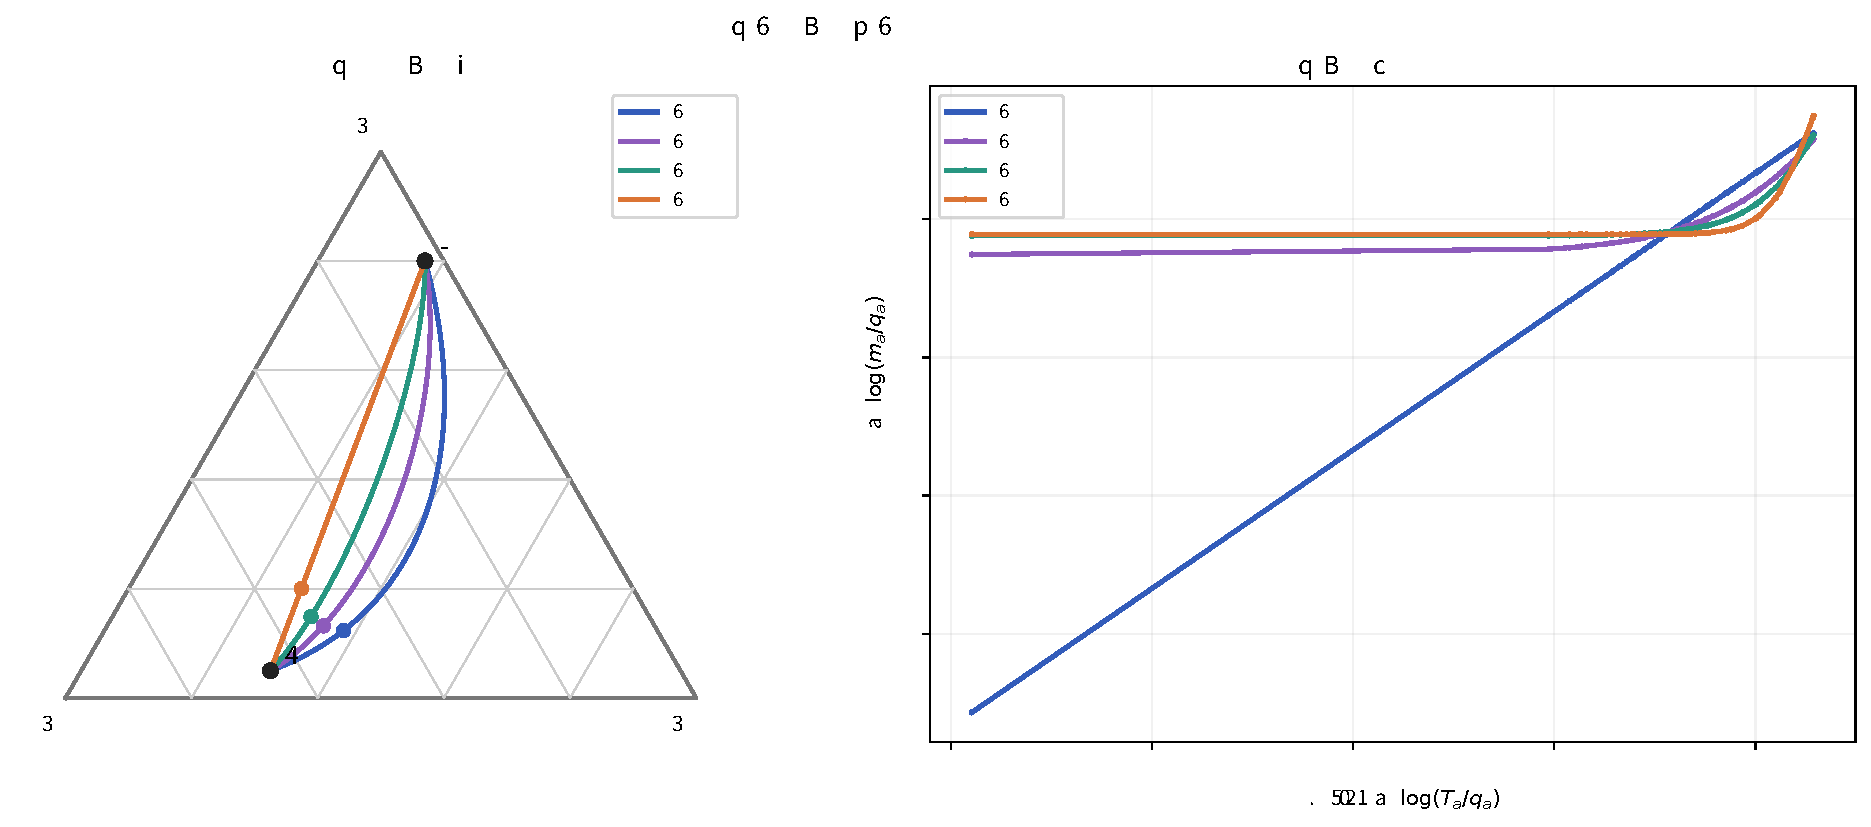
\includegraphics[width=\textwidth]{../../results/proximal-family-geometry/geometry.pdf}
 \caption{幂均值目标的概率路径与 Token 对数概率比。左图圆点均为 $\eta=0.2$；右图以 64 维概率向量展示同一族。形状参数 $\kappa$ 连续改变高维路径和负尾部饱和度。}
\end{figure}

\begin{theorem}[幂均值重心唯一性与超额损失的精确分解]
\label{thm:proximal-barycenter-gap}
对 $0<\kappa<1$，定义加权幂散度重心泛函：
\begin{equation}
 F(p)=(1-\eta)D_\kappa(q\Vert p)+\eta D_\kappa(t\Vert p).
 \label{eq:proximal-divergence-barycenter}
\end{equation}
其在概率单纯形上的唯一全局最小点恰为式~\eqref{eq:proximal-power-target} 的幂均值分布 $m$。且对任意候选分布 $p\in\Delta_V^\circ$，成立如下精确超额损失分解：
\begin{equation}
 F(p)=\frac{1-Z^\kappa}{\kappa(1-\kappa)}+Z^\kappa D_\kappa(m\Vert p),\qquad
 F(p)-F(m)=Z^\kappa D_\kappa(m\Vert p).
 \label{eq:proximal-gap-identity}
\end{equation}
在两个连续端点 $\kappa=0$ 与 $\kappa=1$ 处，超额损失分别为 $\KL(p\Vert m)$ 与 $\KL(m\Vert p)$。进一步，在最优点 $p_\theta=m$ 处，参数化目标的二阶 Hessian 矩阵与局部 Fisher 信息矩阵 $\mathcal I_\theta(m)$ 精确成正比：
\begin{equation}
 \nabla_\theta^2 F(p_\theta)\big|_{p_\theta=m}
 =Z^\kappa J_\theta^\top\operatorname{diag}(1/m)J_\theta
 =Z^\kappa\mathcal I_\theta(m).
 \label{eq:proximal-fisher-hessian}
\end{equation}
对于多个固定教师分布 $\{t^{(j)}\}$ 及非负权重 $\sum_j w_j=1$，重心同样满足 $\argmin_p\sum_j w_j D_\kappa(t^{(j)}\Vert p)\propto\bigl[\sum_j w_j(t^{(j)})^\kappa\bigr]^{1/\kappa}$。
\end{theorem}
\begin{proof}
令 $S_a=(1-\eta)q_a^\kappa+\eta t_a^\kappa=Z^\kappa m_a^\kappa$，则 $F(p)=\frac{1-\sum_a S_a p_a^{1-\kappa}}{\kappa(1-\kappa)}$。引入归一化乘子 $\nu$，一阶条件 $-\frac{S_a}{\kappa}p_a^{-\kappa}+\nu=0\implies p_a\propto S_a^{1/\kappa}=h_a$，归一化即得唯一解 $m$。将 $S_a=Z^\kappa m_a^\kappa$ 代入 $F(p)$：
\begin{equation*}
 F(p)=\frac{1-Z^\kappa\sum_a m_a^\kappa p_a^{1-\kappa}}{\kappa(1-\kappa)}
 =\frac{1-Z^\kappa}{\kappa(1-\kappa)}+Z^\kappa D_\kappa(m\Vert p).
\end{equation*}
令 $p=m$ 得 $F(m)=(1-Z^\kappa)/[\kappa(1-\kappa)]$，相减即得式~\eqref{eq:proximal-gap-identity}。在 $p=m$ 处，概率坐标 Hessian 为 $\operatorname{diag}(S_a m_a^{-\kappa-1})=Z^\kappa\operatorname{diag}(1/m_a)$，结合一阶驻点条件经链式法则即得式~\eqref{eq:proximal-fisher-hessian}。
\end{proof}

\begin{figure}[htbp]
 \centering
 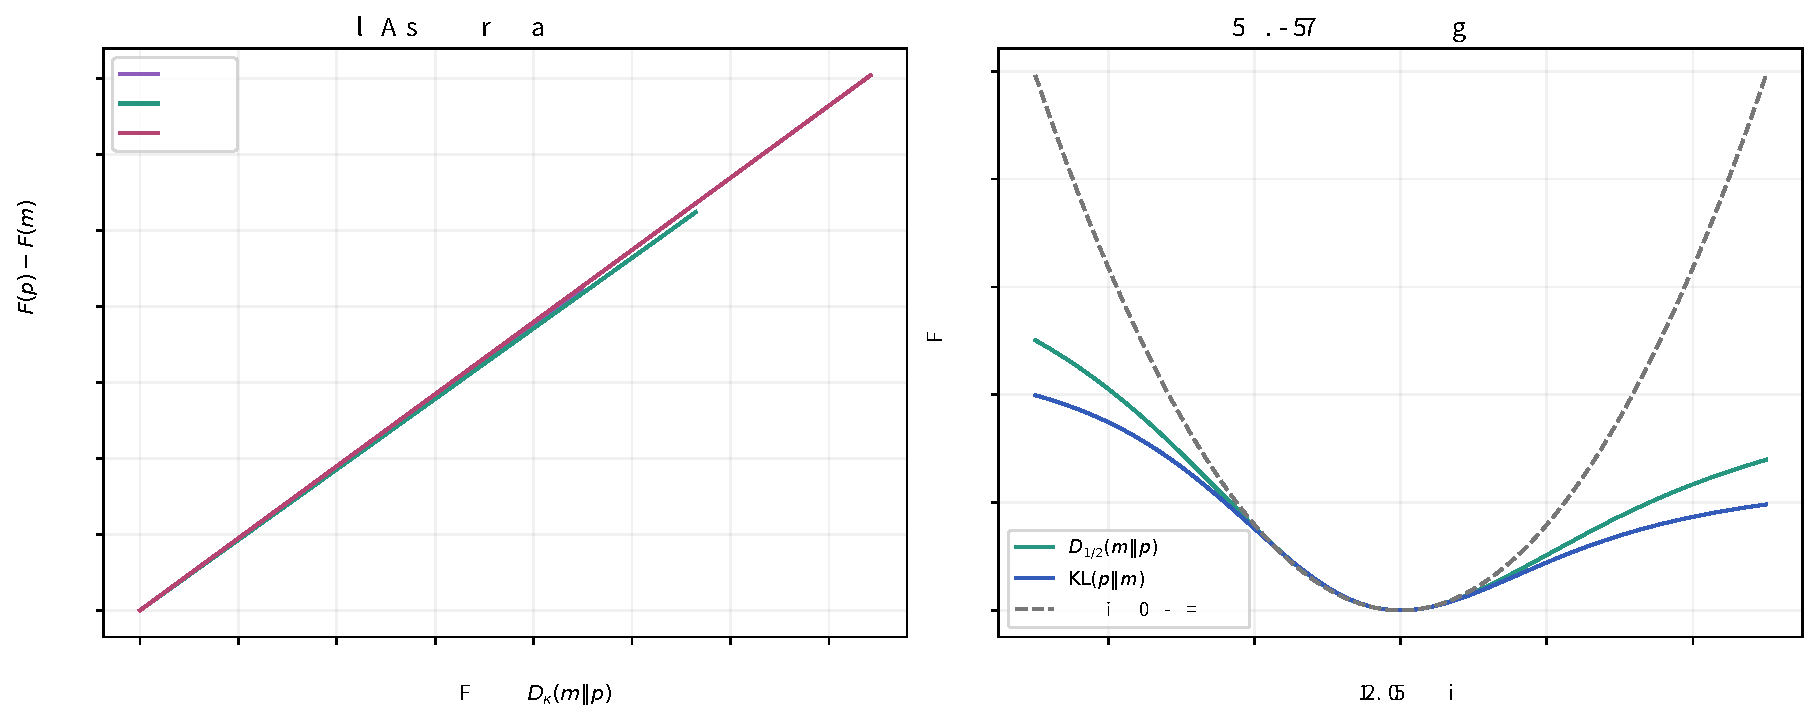
\includegraphics[width=\textwidth]{../../results/proximal-family-geometry/decomposition.pdf}
 \caption{左图检验超额损失精确恒等式 $F(p)-F(m)=Z^\kappa D_\kappa(m\Vert p)$，所有点位于对应常数斜率 $Z^\kappa$ 的直线上。右图固定同一个平方根目标，比较 Hellinger 与逆向 KL 拟合。}
\end{figure}

\section{精确镜像下降（MD）的全局教师目标}
\label{sec:proximal-md-objective}

幂均值重心定义了本轮目标 $m$，但我们还需回答：\textbf{当外层反复将锚点更新为 $q_{k+1}=m_{\kappa,\eta}(q_k,t)$ 时，整个外层迭代究竟在最小化哪一个不依赖锚点 $q$ 的固定教师目标泛函？} 本节通过逆向积分精确构造出这一目标泛函 $\mathcal J_{\kappa,\eta}(p;t)$。

\begin{theorem}[幂均值信号的可积性与精确镜像下降（MD）教师目标]
\label{thm:power-md-integrable-objective}
记 $A(x)=A_{\kappa,\eta}(x)=\frac{\log(1-\eta+\eta x^\kappa)}{\kappa\eta}$，定义规范化凸生成函数与全局教师目标泛函：
\begin{equation}
 \omega_{\kappa,\eta}(x)
 =x\int_1^x\frac{A_{\kappa,\eta}(u)}{u^2}\,du
 \quad (x>0),
 \qquad
 \mathcal J_{\kappa,\eta}(p;t)
 =D_{\omega_{\kappa,\eta}}(t\Vert p)
 =\sum_{a\in\mathcal V} p_a\omega_{\kappa,\eta}\!\left(\frac{t_a}{p_a}\right).
 \label{eq:power-md-generator-integral,eq:power-md-fixed-objective}
\end{equation}
则 $\omega_{\kappa,\eta}(1)=\omega_{\kappa,\eta}'(1)=0$、曲率满足
\begin{equation}
 \omega_{\kappa,\eta}''(x)=\frac{A_{\kappa,\eta}'(x)}{x}
 =\frac{x^{\kappa-2}}{1-\eta+\eta x^\kappa}>0,
 \label{eq:power-md-curvature}
\end{equation}
故 $\mathcal J_{\kappa,\eta}(p;t)\ge 0$ 且唯一零点为 $p=t$。在开单纯形 $\Delta_V^\circ$ 上，$\mathcal J_{\kappa,\eta}$ 关于 $p_a$ 的偏导数恒为
\begin{equation}
 \frac{\partial\mathcal J_{\kappa,\eta}}{\partial p_a}(p;t)
 =-A_{\kappa,\eta}\!\left(\frac{t_a}{p_a}\right).
 \label{eq:power-md-exact-gradient}
\end{equation}
因此，在锚点 $q$ 处对固定教师目标 $\mathcal J_{\kappa,\eta}(\cdot;t)$ 执行步长为 $\eta$ 的标准负熵镜像下降步：
\begin{equation}
 p^+=\argmin_{p\in\Delta_V}
 \left\{\bigl\langle\nabla_p\mathcal J_{\kappa,\eta}(q;t),\,p-q\bigr\rangle
       +\frac1\eta\KL(p\Vert q)\right\},
 \label{eq:power-md-exact-step}
\end{equation}
其唯一最优解精确等于幂均值目标分布 $m_{\kappa,\eta}(q,t)$。
\end{theorem}
\begin{proof}
对 $\omega(x)=x\int_1^x A(u)u^{-2}\,du$ 求导，得 $\omega'(x)=\int_1^x A(u)u^{-2}\,du+A(x)/x$，从而透视导数满足恒等式
\begin{equation*}
 \frac{\partial}{\partial p_a}\bigl[p_a\omega(t_a/p_a)\bigr]
 =\omega(x)-x\omega'(x)=-A(x),\qquad x=\frac{t_a}{p_a}.
\end{equation*}
再对 $\omega'(x)$ 求导得 $\omega''(x)=A'(x)/x=x^{\kappa-2}/(1-\eta+\eta x^\kappa)>0$。由于 $A(1)=0$，自动满足规范化条件 $\omega(1)=\omega'(1)=0$。将该精确梯度 $\nabla_p\mathcal J_{\kappa,\eta}(q;t)=-A_{\kappa,\eta}(t/q)$ 代入负熵镜像步~\eqref{eq:power-md-exact-step}，由定理~\ref{thm:ch2-gibbs} 立得 $p_a^+\propto q_a\exp[\eta A_{\kappa,\eta}(t_a/q_a)]=q_a\exp[f_{\kappa,\eta}(\log(t_a/q_a))]=h_a$，归一化后恰为 $m_{\kappa,\eta}(q,t)$。
\end{proof}

\begin{proposition}[一般单调概率比信号的可积性与相对光滑框架]
\label{prop:power-general-signal-framework}
对任意满足 $S(1)=0$、$S'(x)>0$ 的连续可微信号函数 $S:(0,\infty)\to\R$，定义 $\omega_S(x)=x\int_1^x S(u)u^{-2}\,du$ 与 $\mathcal J_S(p;t)=D_{\omega_S}(t\Vert p)$，均满足 $\nabla_p\mathcal J_S(p;t)=-S(t/p)$。若 $L_S=\sup_{x>0}x S'(x)<\infty$，则 $\mathcal J_S$ 相对于负熵势 $H(p)=\sum_a p_a\log p_a$ 是 $L_S$-相对光滑的（因为 $\nabla_p^2\mathcal J_S=\operatorname{diag}[x_a S'(x_a)/p_a]\preceq L_S\nabla^2 H(p)$），且对任意步长 $0<\tau\le 1/L_S$ 的熵 MD 均具有单步下降与 $O(1/K_{\mathrm{out}})$ 收敛保证。对幂均值信号 $A_{\kappa,\eta}$，恰有 $\sup_{x>0}x A_{\kappa,\eta}'(x)=\sup_{x>0}\frac{x^\kappa}{1-\eta+\eta x^\kappa}=\frac1\eta$。
\end{proposition}

\begin{theorem}[精确 MD 目标的极限端点、加权 JS 表示、调和曲率与锐统一上界]
\label{thm:power-md-objective-endpoints}
\label{thm:power-md-uniform-cap}
固定正支持分布时，$\mathcal J_{\kappa,\eta}(p;t)$ 具有如下解析性质：
\begin{enumerate}
\item \textbf{极限端点与算术 JS 闭式解}：
\begin{equation}
 \mathcal J_{0,\eta}(p;t)=\lim_{\eta\to 1}\mathcal J_{\kappa,\eta}(p;t)=\KL(p\Vert t),\qquad
 \lim_{\eta\to 0}\mathcal J_{\kappa,\eta}(p;t)=D_\kappa(t\Vert p).
 \label{eq:power-md-objective-limits}
\end{equation}
在算术形状 $\kappa=1$ 且固定 $0<\eta<1$ 时，记混合分布 $M=(1-\eta)p+\eta t$，目标闭式解为归一化加权 Jensen--Shannon（JS）散度：
\begin{equation}
 \boxed{\mathcal J_{1,\eta}(p;t)
 =\frac{(1-\eta)\KL(p\Vert M)+\eta\KL(t\Vert M)}{\eta(1-\eta)}.}
 \label{eq:power-md-js-endpoint}
\end{equation}
\item \textbf{生成函数曲率的调和平均律}：对一切 $x>0$，
\begin{equation}
 \frac1{\omega_{\kappa,\eta}''(x)}
 =\frac{1-\eta}{g_\kappa''(x)}+\frac\eta{g_0''(x)}.
 \label{eq:power-md-harmonic-curvature}
\end{equation}
\item \textbf{分布无关的锐统一上界}：当 $0<\kappa\le 1$ 且 $0<\eta<1$ 时，定义正常数
\begin{equation}
 c=-\frac{\log(1-\eta)}{\kappa\eta},\qquad
 d=\int_1^\infty\frac{A_{\kappa,\eta}(u)}{u^2}\,du\in\left(0,\frac1\eta\right],
\end{equation}
则对任意词表维数与任意正支持分布恒有锐界：
\begin{equation}
 0\le\mathcal J_{\kappa,\eta}(p;t)\le c+d
 \qquad\left(\kappa=1\text{ 时 }c+d=\frac{-\eta\log\eta-(1-\eta)\log(1-\eta)}{\eta(1-\eta)}\right).
 \label{eq:power-md-uniform-cap}
\end{equation}
\end{enumerate}
\end{theorem}
\begin{proof}
极限式由控制收敛定理直接得出；对 $\kappa=1$ 分部积分得 $\omega_{1,\eta}(x)=\frac{\eta x\log x-(1-\eta+\eta x)\log(1-\eta+\eta x)}{\eta(1-\eta)}$，代入求和即得式~\eqref{eq:power-md-js-endpoint}。曲率式~\eqref{eq:power-md-harmonic-curvature} 由 $1/\omega''(x)=(1-\eta)x^{2-\kappa}+\eta x^2=(1-\eta)/g_\kappa''(x)+\eta/g_0''(x)$ 直接给出。最后，当 $x\to 0^+$ 时 $\omega(x)\to c$，当 $x\to\infty$ 时渐近斜率 $\omega(x)/x\to d\le\int_1^\infty(\log u)/(\eta u^2)\,du=1/\eta$。由凸性知 $\omega(x)\le c+dx$，对 $x=t/p$ 求 $p$-期望即得 $\mathcal J_{\kappa,\eta}(p;t)\le c+d$；取 $p=(\epsilon,1-\epsilon), t=(1-\epsilon,\epsilon)$（$\epsilon\downarrow 0$）即逼近上确界 $c+d$。
\end{proof}

\begin{center}
\small
\begin{tabular}{lll}
\toprule
散度对象及其在框架中的职责 & 几何端点 $\kappa=0$ & 算术端点 $\kappa=1$（固定 $0<\eta<1$）\\
\midrule
$D_\kappa(t\Vert p)$：定义幂均值重心 & $\KL(p\Vert t)$ & $\KL(t\Vert p)$\\
$\mathcal J_{\kappa,\eta}(p;t)$：精确外层 MD 教师目标 & $\KL(p\Vert t)$ & $\mathrm{JS}_\eta(p,t)/[\eta(1-\eta)]$\\
$K_{\kappa,\eta}(q,t)$：BPO 冻结教师中心 & $\KL(q\Vert t)$ & $\KL(q\Vert(1-\eta)q+\eta t)/\eta$\\
\bottomrule
\end{tabular}
\end{center}

\begin{theorem}[精确幂均值 MD 的全局相对光滑性、单步下降与 $O(1/(\eta K_{\mathrm{out}}))$ 收敛率]
\label{thm:power-md-relative-smoothness}
固定教师 $t$ 与 $(\kappa,\eta)$，令负熵为 $H(p)=\sum_a p_a\log p_a$。在开单纯形 $\Delta_V^\circ$ 上，$\mathcal J=\mathcal J_{\kappa,\eta}(\cdot;t)$ 相对于 $H$ 具有常数 $1/\eta$ 的全局相对光滑性：
\begin{equation}
 \mathcal J(p;t)\le\mathcal J(q;t)+\bigl\langle\nabla\mathcal J(q;t),\,p-q\bigr\rangle
       +\frac1\eta\KL(p\Vert q).
 \label{eq:power-md-relative-smoothness}
\end{equation}
若单步更新为 $p^+\propto q\exp[\tau A_{\kappa,\eta}(t/q)]$（其中步幅满足 $0<\tau\le\eta$），则成立单步下降与三点进展不等式：
\begin{align}
 \mathcal J(q;t)-\mathcal J(p^+;t)
 &\ge\frac1\tau\KL(q\Vert p^+)
  +\left(\frac1\tau-\frac1\eta\right)\KL(p^+\Vert q)\ge 0,\\
 \tau\mathcal J(p^+;t)
 &\le\KL(t\Vert q)-\KL(t\Vert p^+).
 \label{eq:power-md-single-step-progress}
\end{align}
对每轮刷新锚点的精确外层迭代 $q_{k+1}=p^+(q_k)$（$0<\tau_k\le\eta$），经过 $K_{\mathrm{out}}$ 轮后的末步（last-iterate）目标误差满足：
\begin{equation}
 \mathcal J(q_{K_{\mathrm{out}}};t)\le
 \frac{\KL(t\Vert q_0)}{\sum_{k=0}^{K_{\mathrm{out}}-1}\tau_k}
 \qquad\left(\text{当 }\tau_k\equiv\eta\text{ 时，}\mathcal J(q_{K_{\mathrm{out}}};t)\le\frac{\KL(t\Vert q_0)}{\eta K_{\mathrm{out}}}\right).
 \label{eq:power-md-last-iterate-rate}
\end{equation}
\end{theorem}
\begin{proof}
记 $x_a=t_a/p_a$，由式~\eqref{eq:power-md-curvature} 可得单纯形上的对角 Hessian 上界：
\begin{equation}
 \nabla_p^2\mathcal J(p;t)
 =\operatorname{diag}\left(\frac1{p_a}
       \frac{x_a^\kappa}{1-\eta+\eta x_a^\kappa}\right)
 \preceq\frac1\eta\operatorname{diag}\left(\frac1{p_a}\right)
 =\frac1\eta\nabla^2 H(p).
 \label{eq:power-md-hessian-bound}
\end{equation}
沿连接 $q,p$ 的线段积分二阶泰勒余项即得相对光滑式~\eqref{eq:power-md-relative-smoothness}。设 $g=\nabla\mathcal J(q;t)$，MD 一阶条件给出 $\langle g,p^+-q\rangle=-\tau^{-1}[\KL(p^+\Vert q)+\KL(q\Vert p^+)]$，代入式~\eqref{eq:power-md-relative-smoothness} 即得第一个单步下降式。再利用 $\mathcal J$ 的凸性 $\mathcal J(q;t)\le\mathcal J(t;t)+\langle g,q-t\rangle=\langle g,q-t\rangle$ 以及 Bregman 三点恒等式 $\langle g,p^+-t\rangle=\tau^{-1}[\KL(t\Vert q)-\KL(t\Vert p^+)-\KL(p^+\Vert q)]$，代入相对光滑式即得式~\eqref{eq:power-md-single-step-progress}。对 $k=0,\ldots,K_{\mathrm{out}}-1$ 望远镜求和，并利用 $\mathcal J(q_k;t)$ 的单调非增性，即得末步收敛率~\eqref{eq:power-md-last-iterate-rate}。
\end{proof}

\subsection{小步连续极限下的自然梯度流与固定幂散度 MD 变体}

当 $\eta\to 0^+$ 时，记 $a_\kappa=\E_q[\rho^\kappa]$，将 $h_a=q_a[1+\eta(\rho_a^\kappa-1)/\kappa+O(\eta^2)]$ 归一化，得到幂均值更新的一阶切向量：
\begin{equation}
 m_a=q_a+\eta v_{\kappa,a}+O(\eta^2),\qquad
 v_{\kappa,a}=\frac{q_a}{\kappa}\bigl(\rho_a^\kappa-a_\kappa\bigr)
 =-\bigl(\operatorname{grad}_{\!F} D_\kappa(t\Vert q)\bigr)_a.
 \label{eq:proximal-natural-velocity}
\end{equation}
在连续流时间 $\tau_{\mathrm{flow}}$ 下，自然梯度流 $\frac{dq_a}{d\tau_{\mathrm{flow}}}=v_{\kappa,a}$ 满足精确 Lyapunov 耗散方程：
\begin{equation}
 \frac{d}{d\tau_{\mathrm{flow}}}D_\kappa(t\Vert q)
 =-\|v_\kappa\|_F^2
 =-\frac1{\kappa^2}\Var_q(\rho^\kappa).
 \label{eq:proximal-flow-lyapunov}
\end{equation}
若在有限步长 $\tau>0$ 下直接对固定幂散度 $D_\kappa(t\Vert q)$ 执行负熵 MD，所得分布为
\begin{equation*}
\widetilde m_a\propto q_a\exp\biggl(\tau\frac{(t_a/q_a)^\kappa-1}{\kappa}\biggr).
\end{equation*}
它在指数内部重新暴露了无界幂函数 $(t_a/q_a)^\kappa$，丧失了幂均值目标 $m_{\kappa,\eta}$ 的对数饱和结构。

\section{单 Rollout 的幂均值 BPO 算法与理想内层路径保证}
\label{sec:power-bpo-algorithm}

将幂均值信号 $f_a=f_{\kappa,\eta}(\log(t_a/q_a))$（等价于归一化信号 $A_{\kappa,\eta}(a)=f_a/\eta$）代入第~\ref{ch:foundations} 章的 KL 镜像子问题：
\begin{equation}
 m=\argmax_{p\in\Delta_V}
 \left\{\sum_{a\in\mathcal V} p_a A_{\kappa,\eta}(a)
       -\frac1\eta\KL(p\Vert q)\right\},
 \qquad m_a=\frac{q_a e^{f_a}}{Z},\quad Z=\sum_b q_b e^{f_b}.
 \label{eq:power-bpo-mirror-subproblem,eq:power-bpo-explicit-target}
\end{equation}
因此，在 BPO 内层中引入幂均值目标\textbf{只需替换两个冻结标量}：将原始动作信号 $r_a$ 替换为 $A_{\kappa,\eta}(a)$，并将冻结教师中心 $\KL(q\Vert t)$ 替换为 $K_{\kappa,\eta}=-\E_q[A_{\kappa,\eta}]$。残差、总体损失与精确梯度分别为：
\begin{align}
 R_\theta(a)&=U_\theta(a)-f_a-\E_q[U_\theta-f]
            =C_q\log\frac{p_\theta}{m}(a),\\
 \frac{R_\theta(a)}{\eta}
 &=\frac{U_\theta(a)+\KL(q\Vert p_\theta)}{\eta}-A_{\kappa,\eta}(a)-K_{\kappa,\eta},\\
 \mathcal L_k(\theta)
 &=\E_{s\sim\widehat d_k}\frac1{2\eta}
     \E_{a\sim q_k(\cdot\mid s)}\bigl[R_\theta(s,a)^2\bigr],\qquad
 \nabla_\theta\mathcal L_s=\frac1\eta\E_q\bigl[R_\theta\psi_\theta\bigr].
 \label{eq:power-bpo-population-loss,eq:power-bpo-gradient}
\end{align}
在独立 Categorical Logits $z$ 下，BPO 的二阶曲率恒为 $\nabla_z^2\mathcal L_s=F_q/\eta$，完全独立于形状参数 $\kappa$：形状参数 $\kappa$ 改变的是回归目标的位置 $\log m$ 与初始残差尾部，而不改变该二次回归的条件数。

\subsection{锚点 Fisher 预条件 BPO 的有限步全 \texorpdfstring{$f$}{f}-散度单调性}

如第~\ref{sec:power-bpo-algorithm} 节构造的三元反例所示（取 $q=(0.4999995,0.4999995,10^{-6}), t=(0.8,0.199999,10^{-6}), \eta=0.3, \kappa=0.5$，在稀有第三动作上扰动 Logit 使 $p\propto m\exp(0,0,12)$，BPO 损失从 $0.06227708$ 降至 $0.00024000$，而 $\KL(p\Vert t)$ 却从 $0.22314483$ 升至 $1.65421904$），任意降低 BPO 损失的候选点并不自动改善教师散度。然而，若沿着锚点 Fisher 预条件（或自然梯度）诱导的几何拟合路径前进，则不仅目标散度单调下降，而且\textbf{所有凸生成 $f$-散度均在每一个有限内层步单调非增}！

在独立 Logits 下，使用冻结锚点 Fisher 伪逆 $F_q^\dagger$ 与步幅 $0<\gamma_n\le 1$ 执行更新：
\begin{align}
 z_{n+1}&=z_n-\gamma_n\eta F_q^\dagger\nabla_z\mathcal L_s(z_n)
     =z_n-\gamma_n F_q^\dagger F_q(z_n-\log m),\\
 p_{n+1,a}&\propto p_{n,a}^{1-\gamma_n}m_a^{\gamma_n}.
 \label{eq:power-bpo-anchor-fisher-step}
\end{align}
从初值 $p_0=q$ 出发，记累计拟合进度为 $\xi_n=1-\prod_{h<n}(1-\gamma_h)\in[0,1]$，归纳可知第 $n$ 步内层分布精确位于指数插值路径上：
\begin{equation}
 p_n=p_{\xi_n},\qquad
 p_{\xi,a}=\frac{q_a e^{\xi f_a}}{Z_\xi},\qquad
 \mathcal L_s(p_n)=(1-\xi_n)^2\mathcal L_s(q).
 \label{eq:power-bpo-finite-inner-path}
\end{equation}

\begin{theorem}[幂均值 BPO 理想预条件内层路径的有限步全 $f$-散度进展]
\label{thm:power-bpo-inner-all-f}
\label{cor:power-general-signal-all-f}
在完整正支持、$\kappa\in[0,1]$、$0<\eta\le 1$ 下，对任意满足 $\Phi(1)=0$ 的凸函数 $\Phi:(0,\infty)\to\R$，定义教师 $f$-散度 $D_\Phi(p\Vert t)=\sum_a t_a\Phi(p_a/t_a)$。则沿内层拟合路径 $p_\xi\propto q e^{\xi f_{\kappa,\eta}}$（$0\le\xi\le 1$），$D_\Phi(p_\xi\Vert t)$ 关于 $\xi$ 单调非增：
\begin{equation*}
 \frac{d}{d\xi}D_\Phi(p_\xi\Vert t)\le 0,\qquad \forall\xi\in[0,1].
\end{equation*}
因此，锚点 Fisher 预条件更新~\eqref{eq:power-bpo-anchor-fisher-step} 在每一个有限内层步均同时不增加逆向 KL $\KL(p_n\Vert t)$、正向 KL $\KL(t\Vert p_n)$、总变差 $\TV(p_n,t)$ 与平方 Hellinger 距离 $H^2(p_n,t)$。更一般地，对命题~\ref{prop:power-general-signal-framework} 中满足 $0<\tau\le 1/L_S$ 的任意单调信号 $S$，路径 $p_\xi\propto q\exp[\xi\tau S(t/q)]$ 同样具有该全 $f$-散度单调性。
\end{theorem}
\begin{proof}
记 $r_a=\log(t_a/q_a)$。幂均值信号 $f(r)=f_{\kappa,\eta}(r)$ 关于 $r$ 严格递增，且导数满足 $0<f'(r)=\frac{\eta e^{\kappa r}}{1-\eta+\eta e^{\kappa r}}\le 1$（对一般信号 $f(r)=\tau S(e^r)$ 亦有 $0<f'(r)=\tau e^r S'(e^r)\le\tau L_S\le 1$）。因此，学生对教师的概率比
\begin{equation}
 u_{\xi,a}=\frac{p_{\xi,a}}{t_a}
 =\frac{\exp\bigl[-r_a+\xi f(r_a)\bigr]}{Z_\xi}
\end{equation}
因指数导数 $-1+\xi f'(r)\le 0$ 而作为 $r_a$ 的函数单调非增。当 $\Phi$ 可微且凸时，$\Phi'(u)$ 随 $u$ 单调非减，故复合函数 $\Phi'(u_\xi(r))$ 作为 $r$ 的函数单调非增，与严格递增的 $f(r)$ 具有相反的单调序（反共单调）。利用 $\partial_\xi p_\xi=p_\xi(f-\E_{p_\xi}[f])$ 求导，由 Chebyshev 协方差不等式（或成对反序恒等式）：
\begin{align}
 \frac{d}{d\xi}D_\Phi(p_\xi\Vert t)
 &=\operatorname{Cov}_{p_\xi}\bigl(\Phi'(u_\xi),\,f\bigr)
 =\frac12\sum_{a,b}p_{\xi,a}p_{\xi,b}
   \bigl[\Phi'(u_{\xi,a})-\Phi'(u_{\xi,b})\bigr](f_a-f_b)
 \le 0.
\end{align}
对不可微凸函数（如 $\TV$ 对应的 $\Phi(u)=\frac12|u-1|$），在紧区间上用光滑凸函数一致逼近即得结论。
\end{proof}

\begin{figure}[htbp]
 \centering
 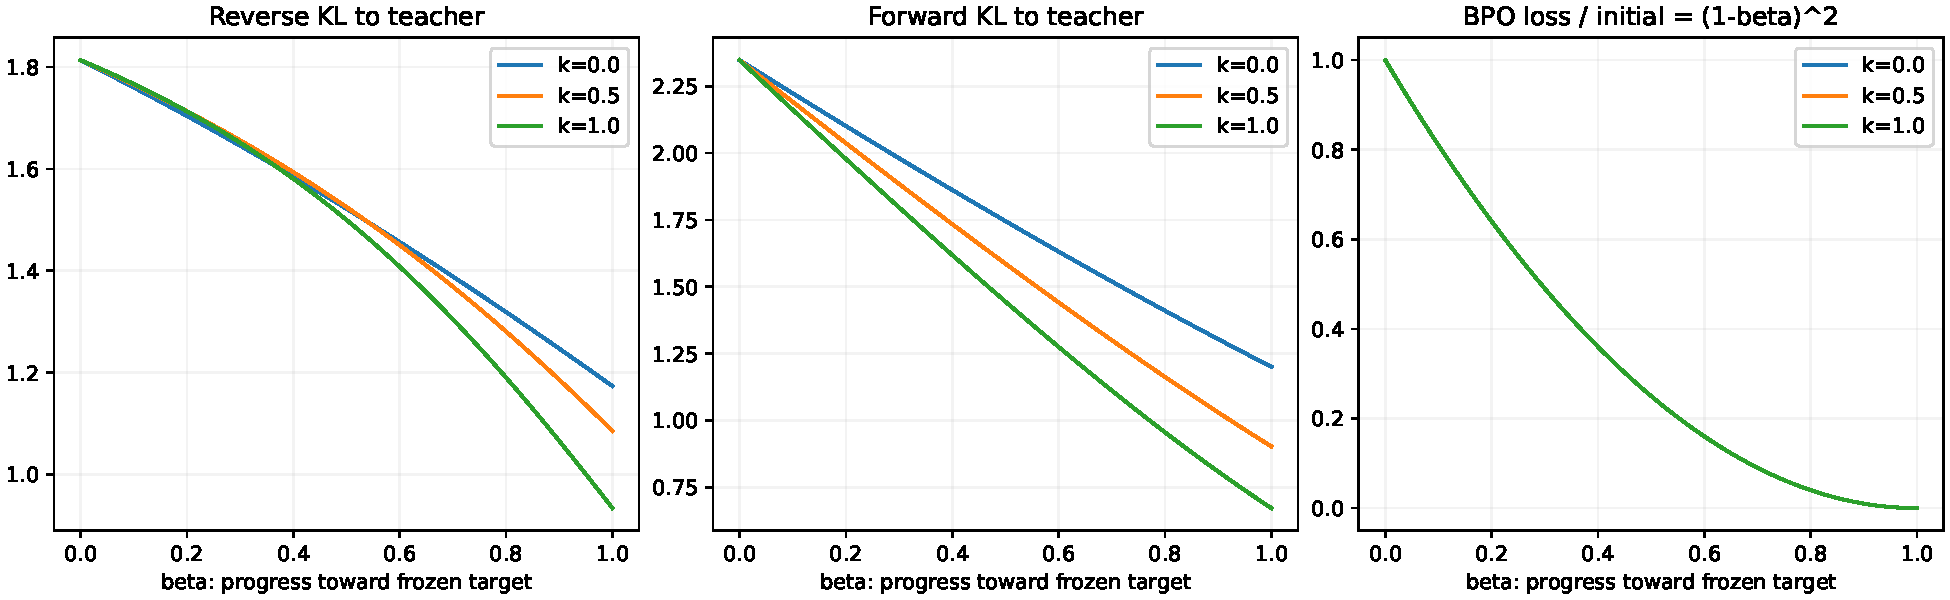
\includegraphics[width=\textwidth]{../../results/power-bpo-algorithm/finite-inner-progress.pdf}
 \caption{理想锚点 Fisher 预条件 BPO 的有限内层路径：双向教师 KL 沿拟合进度 $\xi$（图中旧记号 $\beta$）单调下降，BPO 损失按 $(1-\xi)^2$ 精确收缩。}
\end{figure}

\begin{algorithm}[htbp]
\caption{单 Rollout 的幂均值 BPO 外层--内层参考算法\\{\small\textit{数学语义：每个 Prompt 单条轨迹采样，完整词表条件期望下拟合幂均值目标}}}
\begin{algorithmic}[1]
\Require 教师 $t$，初始参数 $\theta_0$，提示分布 $\mathcal D$，批大小 $B\ge1$，步长 $0<\eta\le1$，形状 $0\le\kappa\le1$，外层轮数 $K_{\mathrm{out}}\ge1$，内层步数 $N\ge1$
\For{outer $k=0,\ldots,K_{\mathrm{out}}-1$}
    \State $q_k\gets\sg(\pi_{\theta_k})$，采样独立提示 $x_1,\ldots,x_B\overset{\mathrm{iid}}\sim\mathcal D$
    \For{每个提示槽位 $x_i$}
        \State 生成单条轨迹 $y_i\sim q_k(\cdot\mid x_i)$，冻结有效前缀与归一化权重 $w_s$
        \For{每个有效前缀 $s$}
            \State 缓存 $q_k(\cdot\mid s)$，$f_s\gets\sg\bigl(f_{\kappa,\eta}(\log(t/q_k))\bigr)$，$\bar f_s\gets\E_{q_k}[f_s]$
        \EndFor
    \EndFor
    \If{存在有效前缀}
        \State $\theta_{k,0}\gets\theta_k$
        \For{$n=0,\ldots,N-1$}
            \State $U_{s,a}\gets\log\bigl(\pi_{\theta_{k,n}}(a\mid s)/q_k(a\mid s)\bigr)$
            \State $R_{s,a}\gets U_{s,a}-f_{s,a}-\E_{q_k}[U_s-f_s]$
            \State $\mathcal L\gets\sum_s w_s\sum_a q_k(a\mid s)R_{s,a}^2/(2\eta)$
            \State $\theta_{k,n+1}\gets\theta_{k,n}-\alpha_{\mathrm{opt}}\nabla_\theta\mathcal L$
        \EndFor
        \State $\theta_{k+1}\gets\theta_{k,N}$ \Comment{内层结束后硬同步更新锚点并刷新下一轮 Rollout}
    \EndIf
\EndFor
\State \Return $\theta_{K_{\mathrm{out}}}$
\end{algorithmic}
\end{algorithm}

\begin{figure}[htbp]
 \centering
 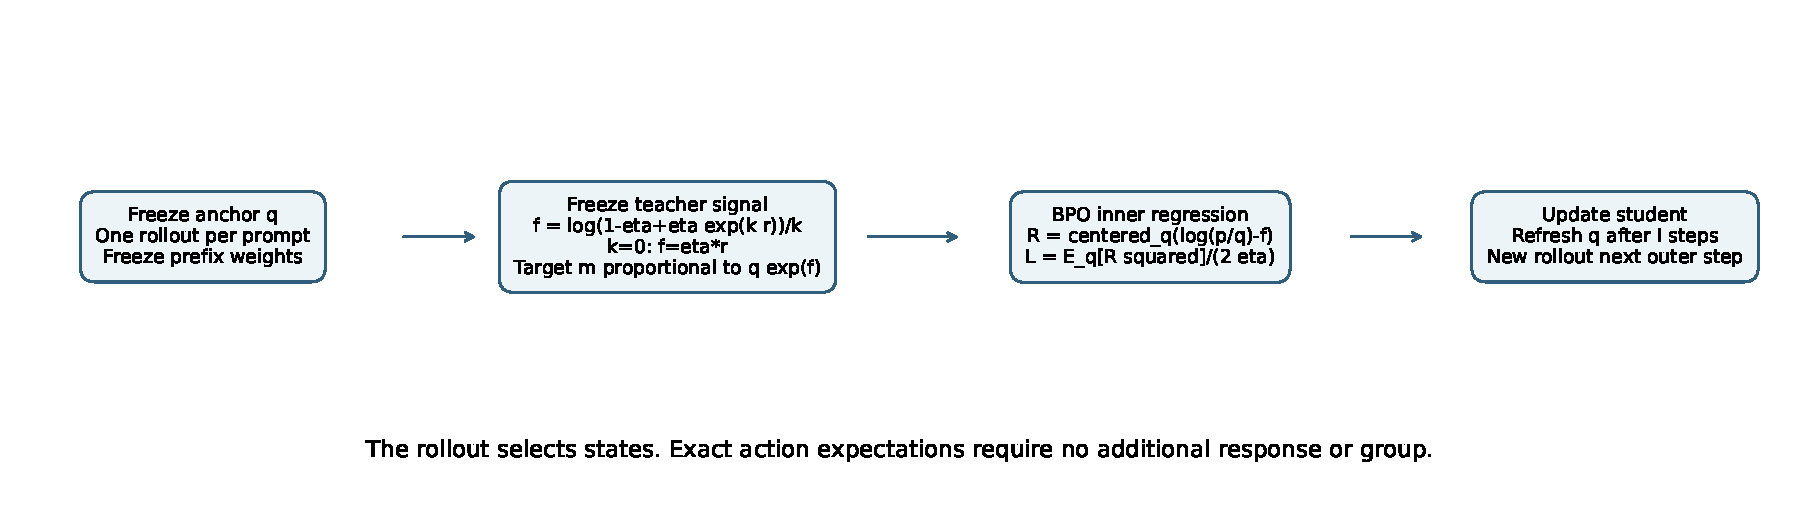
\includegraphics[width=\textwidth]{../../results/power-bpo-algorithm/pipeline.pdf}
 \caption{单条回复轨迹确定前缀，幂均值形状决定冻结监督，BPO 以冻结 $q_k$ 的条件方差拟合目标分布。}
\end{figure}
\begin{figure}[htbp]
 \centering
 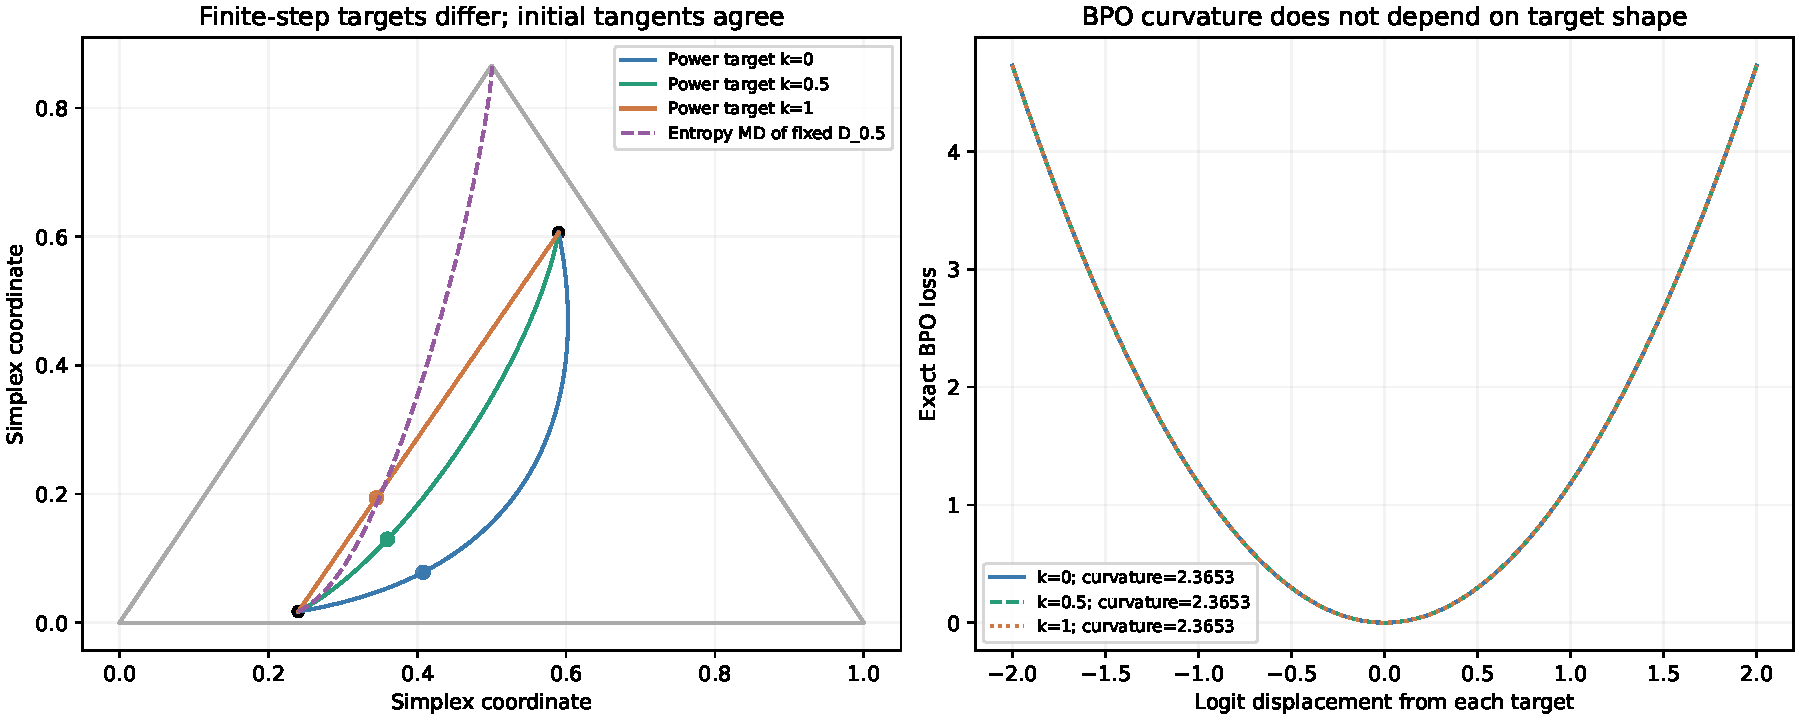
\includegraphics[width=\textwidth]{../../results/power-bpo-algorithm/geometry-and-curvature.pdf}
 \caption{左：幂均值有限步路径与固定 $D_{1/2}$ 的熵 MD 路径仅在起始切向量一致。右：不同目标形状 $\kappa$ 仅平移固定 $q,\eta$ 下的 BPO 二次损失最小点位置，不改变二次曲率。}
\end{figure}

\section{教师监督的方差控制、形状阈值与中心性质}
\label{sec:proximal-teacher-center}

本节研究冻结教师信号 $f_{\kappa,\eta}(r)=\kappa^{-1}\log(1-\eta+\eta e^{\kappa r})$、归一化监督 $A_{\kappa,\eta}=f_{\kappa,\eta}/\eta$、冻结教师中心 $K_{\kappa,\eta}=-\E_q[A_{\kappa,\eta}]$ 以及中心化优势函数 $B_{\kappa,\eta}=A_{\kappa,\eta}+K_{\kappa,\eta}$ 的二阶矩与高阶矩性质。

\subsection{固定插值强度的统一二阶矩界与小步形状阈值}

\begin{theorem}[幂均值信号在固定正 $\eta$ 下的统一二阶矩上界]
\label{thm:proximal-power-variance}
在有限词表且 $q_a,t_a>0$、$0<\kappa\le 1$、$0<\eta<1$ 下，定义有限通用常数与二阶矩界：
\begin{equation}
 C_\star=\sup_{u>0}\frac{\log^2(1+u)}{u}<\infty,\qquad
 B_{\kappa,\eta}=\frac{\log^2(1-\eta)+C_\star\eta}{\kappa^2}.
\end{equation}
则对任意词表维数与任意正支持分布，恒有 $\E_q[f_{\kappa,\eta}^2]\le B_{\kappa,\eta}$ 以及 $\E_q[A_{\kappa,\eta}^2]\le B_{\kappa,\eta}/\eta^2$。若得分范数满足 $\|\psi(a)\|\le S$，则中心化教师得分梯度的协方差迹满足
\begin{equation}
 \Var_q\bigl[\psi C_q A_{\kappa,\eta}\bigr]\le S^2\Var_q(A_{\kappa,\eta})
 \le \frac{S^2 B_{\kappa,\eta}}{\eta^2}.
\end{equation}
反之，在几何端点 $\kappa=0$ 处不存在有限的分布无关上界。
\end{theorem}
\begin{proof}
记 $\rho=t/q$。在负区域 $\rho<1$ 上，因 $\log(1-\eta)/\kappa\le f_{\kappa,\eta}<0$，其平方期望不超过 $\log^2(1-\eta)/\kappa^2$。在正区域 $\rho\ge 1$ 上，$0\le f_{\kappa,\eta}\le\kappa^{-1}\log(1+\eta\rho^\kappa)$，故 $f_{\kappa,\eta}^2\le C_\star\eta\rho^\kappa/\kappa^2$。由于 $0<\kappa\le 1$，$x\mapsto x^\kappa$ 为凹函数，结合 $\E_q[\rho]=1$ 由 Jensen 不等式得 $\E_q[\rho^\kappa]\le 1$。相加即得 $\E_q[f_{\kappa,\eta}^2]\le B_{\kappa,\eta}$。
\end{proof}

当考虑小插值强度极限 $\eta\to 0^+$ 时，若允许最坏情形分布 $(q,t)$ 随 $\eta$ 自由选取，定义完整支持分布类上的最坏信号二阶矩：
\begin{equation}
 \mathcal B_\kappa(\eta)
 =\sup_{q,t\in\Delta_V^\circ}\E_q\left[
 \left(\frac1\kappa\log\bigl(1-\eta+\eta(t/q)^\kappa\bigr)\right)^2
 \right].
\end{equation}

\begin{theorem}[最坏二阶矩与一般 $p$ 阶矩的精确小步形状阈值]
\label{thm:proximal-moment-threshold}
\label{thm:power-general-moment-threshold}
对任意固定形状 $0<\kappa\le 1$，当 $\eta\to 0^+$ 时，最坏未归一化信号二阶矩与归一化监督 $A_{\kappa,\eta}$（及中心化监督 $C_q A_{\kappa,\eta}$）的最坏 $p$ 阶矩（$p\ge 1$）满足精确渐近阶数：
\begin{align}
 \mathcal B_\kappa(\eta)&=\Theta_\kappa\!\left(\eta^{\min\{2,\,1/\kappa\}}\right),
 \label{eq:proximal-sharp-moment-order}\\
 \sup_{q,t}\E_q\bigl|A_{\kappa,\eta}\bigr|^p
 &=\Theta_{\kappa,p}\!\left(\eta^{\min\{p,\,1/\kappa\}-p}\right),
 \qquad
 \sup_{q,t}\E_q\bigl|C_q A_{\kappa,\eta}\bigr|^p
 =\Theta_{\kappa,p}\!\left(\eta^{\min\{p,\,1/\kappa\}-p}\right).
\end{align}
其中隐含常数仅依赖 $(\kappa,p)$ 而与词表维数无关。因此：
\begin{enumerate}
\item 小步极限下归一化监督 $A_{\kappa,\eta}$ 具有 $O_\kappa(1)$ 统一有界二阶矩（即 $\mathcal B_\kappa(\eta)=\Theta_\kappa(\eta^2)$）的\textbf{充要形状区间为 $0<\kappa\le 1/2$}；当 $1/2<\kappa\le 1$ 时，$\sup_{q,t}\Var_q(A_{\kappa,\eta})=\Theta_\kappa(\eta^{1/\kappa-2})\to\infty$。
\item 小步极限下具有统一有界 $p$ 阶矩的\textbf{充要形状区间为 $0<\kappa\le 1/p$}（例如统一四阶矩要求 $0<\kappa\le 1/4$）。
\item 几何端点 $\kappa=0$ 对任意正 $\eta>0$ 均有 $\mathcal B_0(\eta)=\infty$。
\end{enumerate}
\end{theorem}
\begin{proof}
对任意 $p\ge 1$，负区域 $\rho<1$ 对 $\E_q|f|^p$ 的贡献不超过 $|\log(1-\eta)/\kappa|^p=O_{\kappa,p}(\eta^p)$。
\begin{itemize}
\item 当 $p\kappa\le 1$（二阶矩 $p=2$ 时即 $\kappa\le 1/2$）：在正区域 $\rho\ge 1$ 上使用 $\log(1+x)\le x$ 及凹函数 Jensen 不等式 $\E_q[\rho^{p\kappa}]\le(\E_q[\rho])^{p\kappa}=1$，得 $\E_q[|f|^p\mathbf1\{\rho\ge 1\}]\le\frac{\eta^p}{\kappa^p}\E_q[\rho^{p\kappa}]\le\frac{\eta^p}{\kappa^p}=O_{\kappa,p}(\eta^p)$。下界则由任一固定非同分布二元对 $(q\ne t)$ 在 $\eta\to 0$ 时 $A_{\kappa,\eta}\to(\rho^\kappa-1)/\kappa\not\equiv 0$ 给出。
\item 当 $p\kappa>1$（二阶矩 $p=2$ 时即 $1/2<\kappa\le 1$）：令 $s=1/\kappa\in[1,p)$，常数 $C_{p,s}=\sup_{x>0}\frac{\log^p(1+x)}{x^s}<\infty$（因在 $x\to 0$ 按 $x^{p-s}\to 0$，在 $x\to\infty$ 亦趋于 $0$）。正区域期望满足
\begin{equation*}
 \E_q\bigl[|f|^p\mathbf1\{\rho\ge 1\}\bigr]
 \le\frac{C_{p,s}\eta^s}{\kappa^p}\E_q\bigl[\rho^{\kappa s}\bigr]
 =\frac{C_{p,s}\eta^{1/\kappa}}{\kappa^p}\E_q[\rho]
 =\frac{C_{p,s}}{\kappa^p}\eta^{1/\kappa}.
\end{equation*}
为构造匹配下界，取二元分布 $t=(1/2,1/2)$、$q_1=\frac12\eta^{1/\kappa}$、$q_2=1-q_1$。则稀有动作满足 $\rho_1=\eta^{-1/\kappa}$、$f_1=\log(2-\eta)/\kappa$，故 $\E_q|f|^p\ge q_1|f_1|^p=\frac{\eta^{1/\kappa}}{2\kappa^p}\log^p(2-\eta)=\Omega_{\kappa,p}(\eta^{1/\kappa})$。两边同除以 $\eta^p$ 即得 $A=f/\eta$ 及中心化 $C_q A$ 的精确阶数 $\Theta_{\kappa,p}(\eta^{1/\kappa-p})$。
\end{itemize}
\end{proof}

\begin{figure}[htbp]
 \centering
 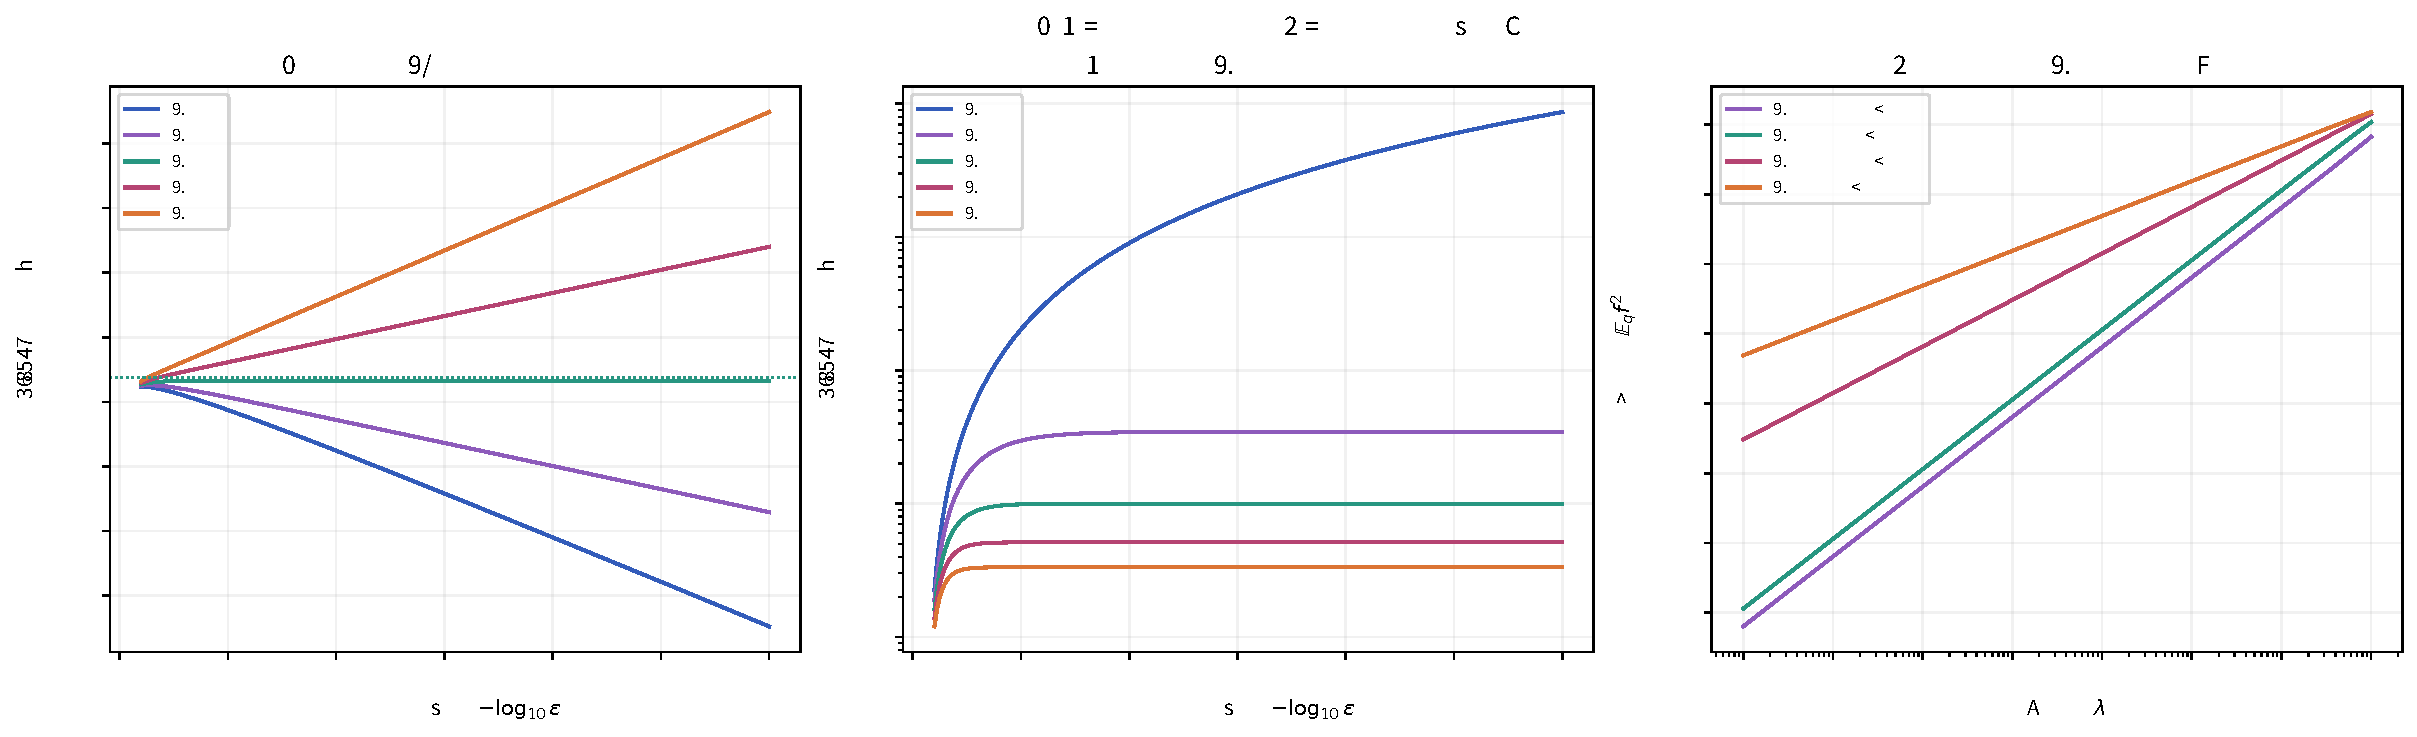
\includegraphics[width=\textwidth]{../../results/proximal-family-geometry/threshold.pdf}
 \caption{形状阈值 $\kappa=1/2$ 的解析见证。左图让学生概率趋零，$\kappa>1/2$ 的自然梯度 Fisher 速度发散；中图让教师概率趋零，几何端点 $\kappa=0$ 的速度发散；右图使用随 $\eta$ 变化的二元锚点，验证二阶矩幂律指数 $\min\{2,1/\kappa\}$（在 $\kappa=0.25,0.5,0.75,1.0$ 处斜率分别为 $2,2,4/3,1$）。}
\end{figure}

\subsection{冻结教师中心 \texorpdfstring{$K_{\kappa,\eta}$}{K_{kappa,eta}} 的凸散度表示、单调性与误差相关方差界}

冻结教师中心显式写为
\begin{equation}
 \boxed{K_{\kappa,\eta}(q,t)
 =-\frac1{\kappa\eta}\sum_{a\in\mathcal V} q_a
 \log\left(1-\eta+\eta\left(\frac{t_a}{q_a}\right)^\kappa\right)
 =\frac{\KL(q\Vert m_{\kappa,\eta})-\log Z}{\eta},}
 \label{eq:center-expanded-k}
\end{equation}
其端点分别为 $K_{0,\eta}=\KL(q\Vert t)$、$K_{1,\eta}=\eta^{-1}\KL(q\Vert(1-\eta)q+\eta t)$ 与 $K_{\kappa,1}=\KL(q\Vert t)$。定义规范化生成函数：
\begin{equation}
 \phi_{\kappa,\eta}(x)=x-1-\frac{\log(1-\eta+\eta x^\kappa)}{\kappa\eta}\quad(x>0),\qquad
 \phi_{\kappa,\eta}''(x)=\frac{x^{\kappa-2}\bigl[(1-\kappa)(1-\eta)+\eta x^\kappa\bigr]}{(1-\eta+\eta x^\kappa)^2}>0.
 \label{eq:center-convex-generator}
\end{equation}
由 $\phi_{\kappa,\eta}(1)=\phi_{\kappa,\eta}'(1)=0$ 及 $\E_q[\rho-1]=0$，可知 $K_{\kappa,\eta}$ 是以 $q$ 为参考测度的严格凸 $f$-散度：
\begin{equation}
 K_{\kappa,\eta}(q,t)=\E_q\bigl[\phi_{\kappa,\eta}(t/q)\bigr]=D_{\phi_{\kappa,\eta}}(t\Vert q).
 \label{eq:divergence-map-center-family}
\end{equation}

\begin{theorem}[教师中心的分布无关锐上界、单调性与小步极限]
\label{thm:center-bounds-monotonicity}
对任意 $0<\kappa\le 1$ 与 $0<\eta<1$，教师中心满足分布无关双侧界：
\begin{equation}
 \frac{1-a_\kappa}{\kappa}\le K_{\kappa,\eta}(q,t)
 \le\min\bigl\{\KL(q\Vert t),\; c_{\kappa,\eta}\bigr\},
 \qquad c_{\kappa,\eta}=-\frac{\log(1-\eta)}{\kappa\eta},\quad a_\kappa=\sum_a q_a^{1-\kappa}t_a^\kappa.
 \label{eq:center-uniform-cap}
\end{equation}
且 $K_{\kappa,\eta}=0\Longleftrightarrow q=t$。对任意固定分布对 $(q,t)$，$K_{\kappa,\eta}$ 关于形状 $\kappa$ 单调非增，关于步长 $\eta$ 单调非减；在任意至少二元的词表上，$c_{\kappa,\eta}$ 是完整支持分布类上的锐上确界。当 $\eta\to 0^+$ 时：
\begin{equation}
 \lim_{\eta\to 0^+}A_{\kappa,\eta}(\rho)=\frac{\rho^\kappa-1}{\kappa},\qquad
 \lim_{\eta\to 0^+}K_{\kappa,\eta}(q,t)=\frac{1-a_\kappa}{\kappa}=(1-\kappa)D_\kappa(t\Vert q),
 \label{eq:divergence-map-center-limit,eq:center-small-step-limit}
\end{equation}
在平方根点 $\kappa=1/2$ 处，$\lim_{\eta\to 0^+}K_{1/2,\eta}(q,t)=2(1-\sum_a\sqrt{q_a t_a})=H^2(q,t)\le 2$。
\end{theorem}
\begin{proof}
上界 $K\le c_{\kappa,\eta}$ 来自逐点 $A(\rho)\ge\log(1-\eta)/(\kappa\eta)=-c_{\kappa,\eta}$；上界 $K\le\KL(q\Vert t)$ 来自加权 AM--GM 不等式 $1-\eta+\eta\rho^\kappa\ge\rho^{\kappa\eta}\implies A(\rho)\ge\log\rho$；下界来自 $\log(1+\eta(\rho^\kappa-1))\le\eta(\rho^\kappa-1)$。对 $k\mapsto H(k)=\log(1-\eta+\eta e^{kr})$，因 $H(0)=0$ 且 $H''(k)=\frac{\eta(1-\eta)r^2 e^{kr}}{(1-\eta+\eta e^{kr})^2}\ge 0$，割线斜率 $H(k)/k$ 非减，故 $K$ 随 $\kappa$ 非增；对 $\eta$ 求导得 $\partial_\eta A=\frac{1-y^{-1}-\log y}{\kappa\eta^2}\le 0$（其中 $y=1-\eta+\eta\rho^\kappa$），故 $K$ 随 $\eta$ 非减。锐性由二元序列 $q=(\epsilon,1-\epsilon), t=(1-\epsilon^2,\epsilon^2)$（$\epsilon\downarrow 0$）达到。
\end{proof}

记中心化教师优势函数的标量条件方差为 $V_{\kappa,\eta}\coloneqq\Var_q(B_{\kappa,\eta})=\Var_q(A_{\kappa,\eta})$（注意跨前缀测度 $d$ 的总体方差满足 $\Var_{d,q}(B)=\E_d[V_s]=\Var_{d,q}(A)-\Var_d(K_s)$，即前缀中心化精确消除了跨前缀均值方差 $\Var_d(K_s)$）。下面的核心定理证明：当 $0<\kappa\le 1/2$ 时，不仅 $V_{\kappa,\eta}$ 一致有界，而且\textbf{随着学生接近教师（$K_{\kappa,\eta}\to 0$），监督方差自动按误差线性归零}！

\begin{theorem}[中心化教师优势函数的误差相关（Error-Scaled）方差控制]
\label{thm:center-advantage-variance}
若 $0<\kappa\le 1/2$ 且 $0<\eta<1$，则条件方差 $V_{\kappa,\eta}$ 同时满足统一常数界与误差相关自界（self-bounding）：
\begin{align}
 V_{\kappa,\eta}
 &\le\frac{1-a_\kappa^2}{\kappa^2(1-\eta)^2}
 \le\frac1{\kappa^2(1-\eta)^2},\\
 V_{\kappa,\eta}
 &\le\frac{D_\kappa(t\Vert q)}{\kappa(1-\eta)^2}
 \le\frac{K_{\kappa,\eta}(q,t)}{\kappa(1-\kappa)(1-\eta)^2}.
 \label{eq:center-error-scaled-variance}
\end{align}
这两个上界均不依赖词表维数或概率分布的最小正下界。特别地，在平方根点 $\kappa=1/2$ 处有 $V_{1/2,\eta}\le\frac{4K_{1/2,\eta}}{(1-\eta)^2}$，且小步极限满足精确恒等式：
\begin{equation}
 \lim_{\eta\to 0^+}V_{1/2,\eta}
 =4\bigl(1-a_{1/2}^2\bigr)=H^2(q,t)\bigl(4-H^2(q,t)\bigr)\le 4.
\end{equation}
\end{theorem}
\begin{proof}
令 $X=\rho^\kappa\ge 0$，$h(X)=\frac{\log(1-\eta+\eta X)}{\kappa\eta}$。在 $X\ge 0$ 上导数满足 $|h'(X)|=\frac{1}{\kappa(1-\eta+\eta X)}\le\frac{1}{\kappa(1-\eta)}$。由独立同分布副本 $X'$ 的成对表示 $\Var(h(X))=\frac12\E[(h(X)-h(X'))^2]\le\frac{\Var_q(X)}{\kappa^2(1-\eta)^2}$。因为 $2\kappa\le 1$，Jensen 不等式给出 $\E_q[\rho^{2\kappa}]\le(\E_q[\rho])^{2\kappa}=1$，故 $\Var_q(X)=\E_q[\rho^{2\kappa}]-a_\kappa^2\le 1-a_\kappa^2$，即得第一式。

为收紧误差相关系数，考察矩生成函数 $a(u)=\E_q[\rho^u]$。由于 $a''(u)=\E_q[\rho^u\log^2\rho]\ge 0$，$a(u)$ 在 $[\kappa,1]$ 上是凸函数。因 $2\kappa\in[\kappa,1]$ 且 $a(1)=1$，弦线不等式给出
\begin{align}
 a(2\kappa)&\le\frac{1-2\kappa}{1-\kappa}a(\kappa)+\frac{\kappa}{1-\kappa},\\
 \Var_q(X)=a(2\kappa)-a(\kappa)^2&\le\frac{\bigl[1-a(\kappa)\bigr]\bigl[\kappa+(1-\kappa)a(\kappa)\bigr]}{1-\kappa}
 \le\frac{1-a(\kappa)}{1-\kappa}.
\end{align}
两边同除以 $\kappa^2(1-\eta)^2$，并代入 $D_\kappa(t\Vert q)=\frac{1-a(\kappa)}{\kappa(1-\kappa)}$ 与定理~\ref{thm:center-bounds-monotonicity} 的下界 $(1-\kappa)D_\kappa(t\Vert q)\le K_{\kappa,\eta}$，即证式~\eqref{eq:center-error-scaled-variance}。
\end{proof}

\begin{figure}[htbp]
 \centering
 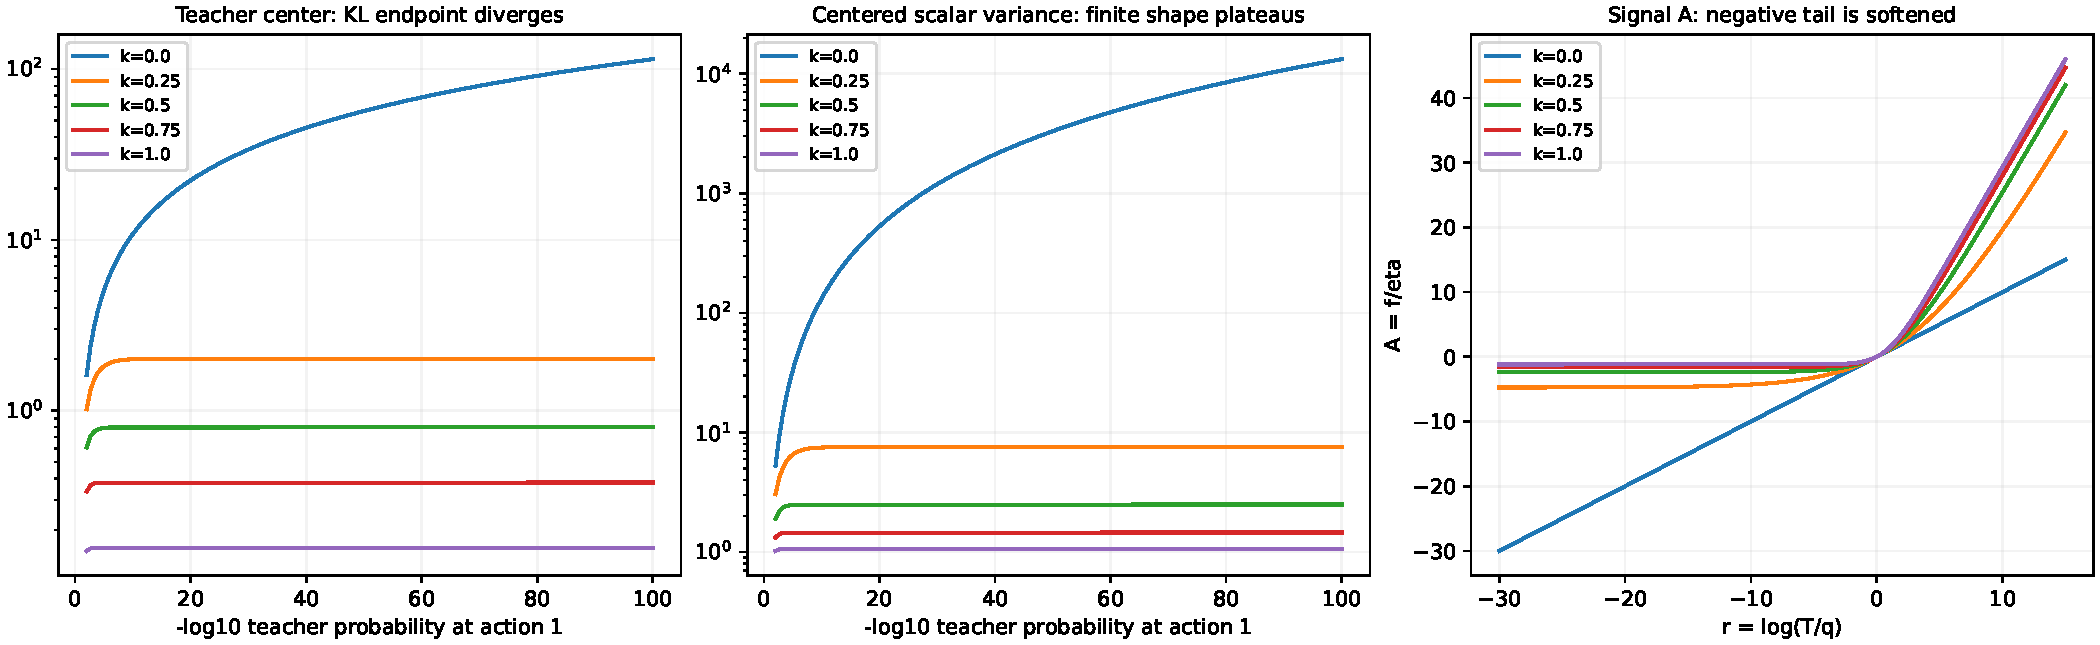
\includegraphics[width=\textwidth]{../../results/power-center-advantage/negative-tail-center-variance.pdf}
 \caption{固定 $q=(1/2,1/2)$、$\eta=0.3$，当教师一个动作概率趋零时，几何中心 $\kappa=0$ 及优势方差无界发散，而正形状 $\kappa>0$ 稳定在有限平台。右图展示规范化信号 $A_{\kappa,\eta}$ 的负尾部饱和效应。}
\end{figure}

\begin{theorem}[教师中心 $K_{\kappa,\eta}$ 与精确 MD 目标 $\mathcal J_{\kappa,\eta}$ 的夹逼等价性及外层可求和方差]
\label{thm:power-md-center-comparison}
\label{cor:power-md-summable-variance}
对任意 $0\le\kappa\le 1$ 与 $0<\eta<1$，生成函数与散度满足全局夹逼不等式：
\begin{equation}
 (1-\kappa)\omega_{\kappa,\eta}(x)\le\phi_{\kappa,\eta}(x)\le\omega_{\kappa,\eta}(x),
 \qquad
 (1-\kappa)\mathcal J_{\kappa,\eta}(q;t)\le K_{\kappa,\eta}(q,t)\le\mathcal J_{\kappa,\eta}(q;t).
 \label{eq:power-md-center-sandwich}
\end{equation}
进一步，当固定 $0<\kappa\le 1/2$ 与 $0<\eta<1$，执行精确幂均值外层更新 $q_{k+1}=m_{\kappa,\eta}(q_k,t)$ 时，记第 $k$ 轮中心化教师优势方差为 $V_k=\Var_{q_k}[B_{\kappa,\eta}(t/q_k)]$，初始正向 KL 为 $C_0=\KL(t\Vert q_0)$，则对任意 $K_{\mathrm{out}}\ge 1$，末步方差与全训练累计方差恒满足：
\begin{equation}
 V_{K_{\mathrm{out}}}\le\frac{C_0}{\kappa(1-\kappa)(1-\eta)^2\eta K_{\mathrm{out}}},
 \qquad
 \sum_{k=1}^{K_{\mathrm{out}}} V_k\le\frac{C_0}{\kappa(1-\kappa)(1-\eta)^2\eta}.
 \label{eq:power-md-summable-variance}
\end{equation}
\end{theorem}
\begin{proof}
比较曲率比值 $\frac{\phi''(x)}{\omega''(x)}=1-\frac{\kappa(1-\eta)}{1-\eta+\eta x^\kappa}\in[1-\kappa,1]$，结合 $x=1$ 处函数值与一阶导数均为零，积分两次即得式~\eqref{eq:power-md-center-sandwich}（注意对 $p$ 求导时，$\frac{\partial}{\partial p_a}K_{\kappa,\eta}(p,t)=-A(x)+\frac{x^\kappa}{1-\eta+\eta x^\kappa}-1\ne -A(x)$，故 $-A$ 是 $\mathcal J$ 的精确梯度而非 $K$ 的梯度）。结合定理~\ref{thm:center-advantage-variance} 的 $V_k\le\frac{K_k}{\kappa(1-\kappa)(1-\eta)^2}\le\frac{\mathcal J(q_k;t)}{\kappa(1-\kappa)(1-\eta)^2}$ 与定理~\ref{thm:power-md-relative-smoothness} 的末步界 $\mathcal J(q_{K_{\mathrm{out}}};t)\le\frac{C_0}{\eta K_{\mathrm{out}}}$ 及望远镜和 $\eta\sum_{k=1}^{K_{\mathrm{out}}}\mathcal J(q_k;t)\le C_0$，立得式~\eqref{eq:power-md-summable-variance}。
\end{proof}

\begin{figure}[H]
 \centering
 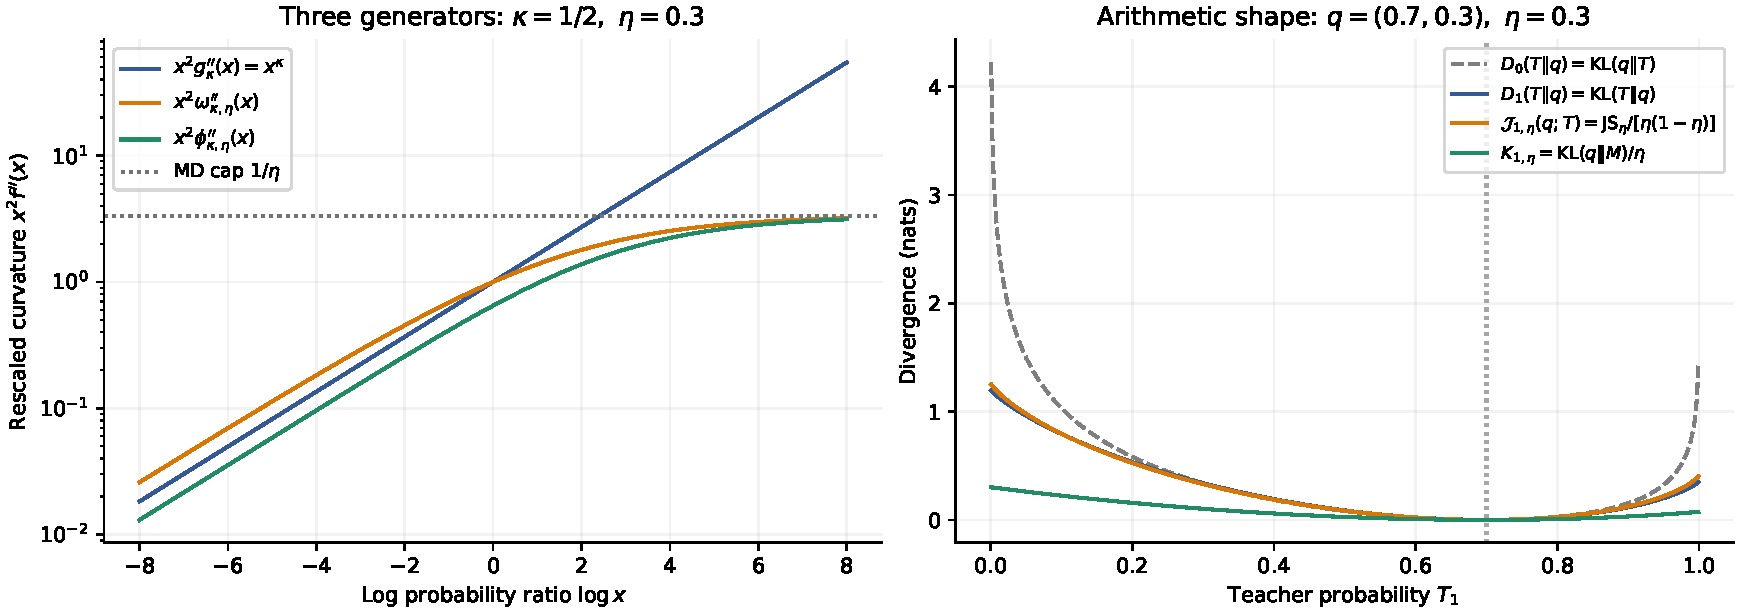
\includegraphics[width=\textwidth]{../../results/power-divergence-relations/families-and-curvature.pdf}
 \caption{三种散度对象的解析比较。左图在 $\kappa=1/2,\eta=0.3$ 时比较乘以 $x^2$ 的生成函数曲率；右图固定 $q=(0.7,0.3),\eta=0.3$，展示算术形状 $\kappa=1$ 下重心散度（正向 KL）、精确 MD 目标（归一化 JS）与教师中心（到混合分布的逆向 KL）的分离。}
 \label{fig:power-divergence-curvature}
\end{figure}

\section{平方根形状（\texorpdfstring{$\kappa=1/2$}{kappa=1/2}）的球面几何与最优性判据}
\label{sec:power-half-and-optimality}

\subsection{自然梯度速度的锐极小极大形状 \texorpdfstring{$\kappa_\star\approx 0.441928$}{kappa_* = 0.441928} 与平方根相对噪声最优性}

由式~\eqref{eq:proximal-natural-velocity}，小步极限下的自然梯度 Fisher 速度平方（亦等于小步标量优势方差 $\lim_{\eta\to 0}V_{\kappa,\eta}$）为 $\|v_\kappa\|_F^2=\Var_q(\rho^\kappa)/\kappa^2$。当 $0<\kappa\le 1/2$ 时，我们可以通过 H\"older 插值求出其在所有完整支持分布上的\textbf{精确解析上确界 $C_{\mathrm{vel}}(\kappa)$}：
令 $X=\rho^\kappa$、$r=1/\kappa\ge 2$，则 $\E_q[X^r]=1$。将 $X^2=X^{(r-2)/(r-1)}(X^r)^{1/(r-1)}$ 施以共轭指数为 $\frac{r-1}{r-2}$ 与 $r-1$ 的 H\"older 不等式，得 $\E_q[X^2]\le(\E_q[X])^{(1-2\kappa)/(1-\kappa)}$。令 $a=\E_q[X]\in[0,1]$，$\gamma=\frac{1-2\kappa}{1-\kappa}$，对凹上界 $a^\gamma-a^2$ 求极值（驻点满足 $a^{2-\gamma}=\gamma/2$），记 $b=\frac{1-2\kappa}{2(1-\kappa)}$，即得锐上确界公式：
\begin{equation}
 \boxed{\sup_{q,t\in\Delta_V^\circ}\|v_\kappa\|_F^2
 =\lim_{\eta\to 0^+}\sup_{q,t}V_{\kappa,\eta}
 =C_{\mathrm{vel}}(\kappa)
 =\frac{b^{1-2\kappa}(1-b)}{\kappa^2},
 \qquad b=\frac{1-2\kappa}{2(1-\kappa)}.}
 \label{eq:proximal-natural-speed-bound}
\end{equation}
该上确界由退化二元序列 $q=(b,1-b), t\to(1,0)$ 逼近达到。对 $\log C_{\mathrm{vel}}(\kappa)$ 使用包络定理求导，令 $\frac{d\log C_{\mathrm{vel}}}{d\kappa}=-\frac2\kappa-2\log b=0$，得到唯一极小极大形状参数方程：
\begin{equation}
 \log\frac{1-2\kappa_\star}{2(1-\kappa_\star)}=-\frac1{\kappa_\star}
 \implies \kappa_\star\approx 0.4419283735,\qquad C_{\mathrm{vel}}(\kappa_\star)\approx 3.5272748442,
\end{equation}
而平方根点 $\kappa=1/2$ 的值为 $C_{\mathrm{vel}}(1/2)=4$。

\begin{figure}[htbp]
 \centering
 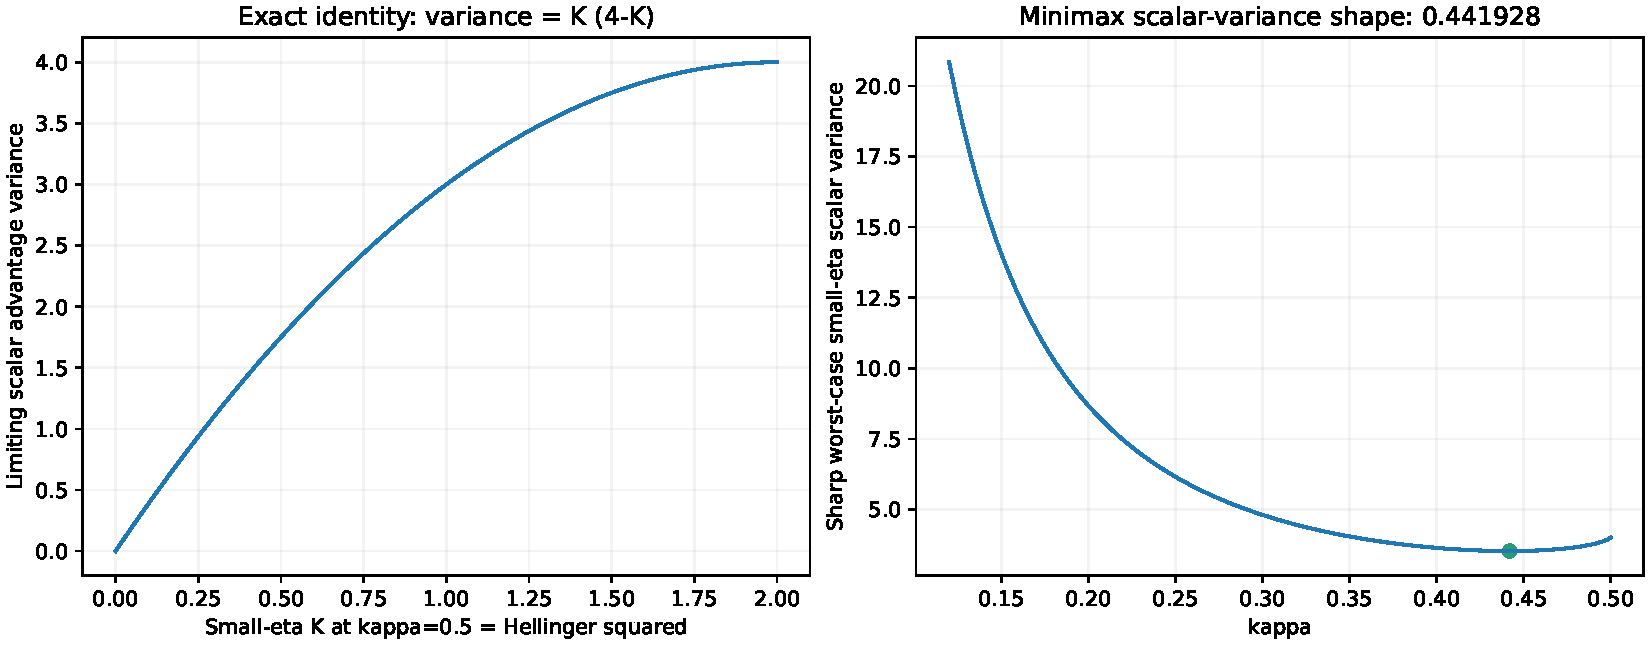
\includegraphics[width=\textwidth]{../../results/power-center-advantage/sharp-small-step-center-variance.pdf}
 \caption{左：平方根形状的小步极限满足精确抛物线关系 $V=K(4-K)$。右：最坏小步标量优势方差（即自然梯度 Fisher 速度平方）的锐常数曲线 $C_{\mathrm{vel}}(\kappa)$，全局最小点位于 $\kappa_\star\approx 0.441928$。}
\end{figure}

相比于绝对方差上界 $C_{\mathrm{vel}}(\kappa)$，若我们考察\textbf{方差相对于当前教师散度误差的放大比率}，则平方根形状 $\kappa=1/2$ 是整个幂散度族中的唯一全局最优解：

\begin{theorem}[平方根形状 $\kappa=1/2$ 的相对误差噪声最优性]
\label{thm:power-relative-noise-optimum}
固定 $0<\kappa\le 1/2$，令小步教师监督为 $A_\kappa^0=(\rho^\kappa-1)/\kappa$，小步中心为 $K_\kappa^0=(1-\E_q[\rho^\kappa])/\kappa$。在至少二元、严格正且 $q\ne t$ 的分布类上取上确界，有精确锐常数：
\begin{align}
 \sup_{q\ne t}\frac{\Var_q(A_\kappa^0)}{D_\kappa(t\Vert q)}&=\frac1\kappa,\\
 \sup_{q\ne t}\frac{\Var_q(A_\kappa^0)}{K_\kappa^0}&=\frac1{\kappa(1-\kappa)}.
 \label{eq:power-relative-noise-sharp}
\end{align}
在全体 $\kappa\in[0,1]$ 中，上述两个相对噪声准则均由平方根形状 $\kappa=1/2$ \textbf{唯一最小化}，对应最小锐常数分别为 $2$ 和 $4$（而 $\kappa=0$ 或 $\kappa>1/2$ 处上确界均为 $+\infty$）。
\end{theorem}
\begin{proof}
上界已由定理~\ref{thm:center-advantage-variance} 证明中 $\Var_q(\rho^\kappa)\le\frac{1-a_\kappa}{1-\kappa}$ 除以 $\kappa^2$ 给出。为证明锐性，取二元序列 $q=(v,1-v), t=(v^2,1-v^2)$（$v\downarrow 0$），此时 $\rho=(v,1+v)$，$a_\kappa=1-(1-\kappa)v+o(v)$，$a_{2\kappa}=1-(1-2\kappa)v+o(v)$，故 $\Var_q(A_\kappa^0)=v/\kappa^2+o(v)$，而 $D_\kappa=v/\kappa+o(v)$、$K_\kappa^0=(1-\kappa)v/\kappa+o(v)$，相除即精确达到 $1/\kappa$ 与 $1/[\kappa(1-\kappa)]$。在区间 $(0,1/2]$ 上两者均严格递减，故唯一最小点均为 $\kappa=1/2$。
\end{proof}

\subsection{平方根形状的连续球面流与离散 \texorpdfstring{$(1-\eta)$}{(1-eta)} 全局 Hellinger 收缩}

在连续时间自然梯度流~\eqref{eq:proximal-flow-lyapunov} 下，当 $\kappa=1/2$ 时，亲和度 $a=\sum_v\sqrt{q_v t_v}$ 满足 $\|v_{1/2}\|_F^2=4(1-a^2)\le 4$ 且 $D_{1/2}(t\Vert q)=4(1-a)$，从而微分方程可精确积分求解：
\begin{equation}
 \frac{da}{d\tau_{\mathrm{flow}}}=1-a^2,
 \qquad a(\tau_{\mathrm{flow}})=\tanh\bigl(\tau_{\mathrm{flow}}+\operatorname{artanh}a(0)\bigr),
 \qquad D_{1/2}(0)e^{-2\tau_{\mathrm{flow}}}\le D_{1/2}(\tau_{\mathrm{flow}})\le D_{1/2}(0)e^{-\tau_{\mathrm{flow}}}.
 \label{eq:proximal-hellinger-flow}
\end{equation}

\begin{figure}[htbp]
 \centering
 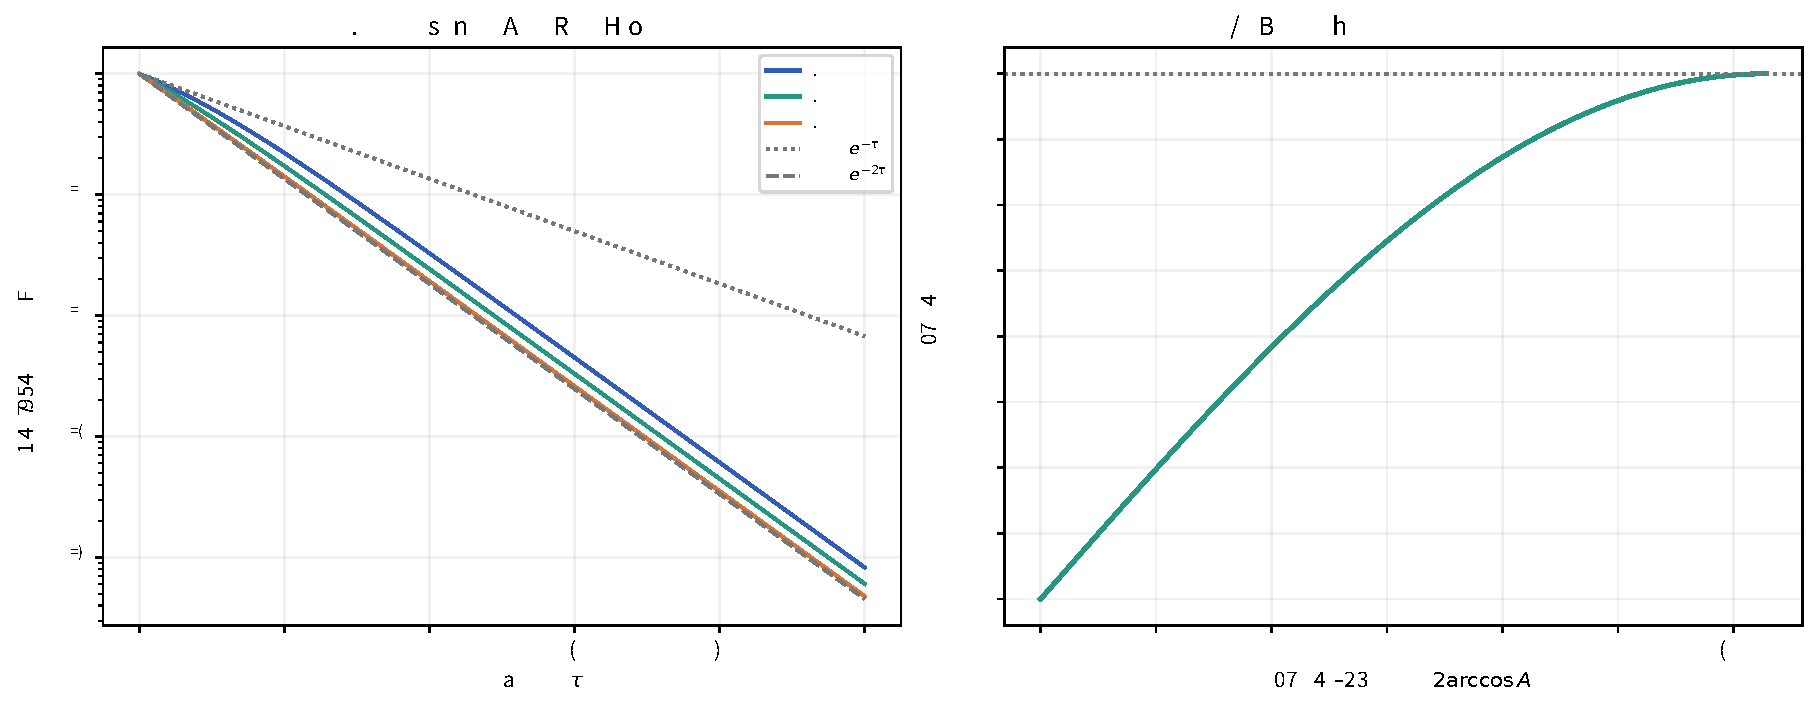
\includegraphics[width=\textwidth]{../../results/proximal-family-geometry/hellinger-flow.pdf}
 \caption{平方根形状的连续自然梯度流动力学。左图由精确解 $a(\tau_{\mathrm{flow}})=\tanh(\tau_{\mathrm{flow}}+\operatorname{artanh}a(0))$ 生成，归一化散度夹在 $e^{-\tau_{\mathrm{flow}}}$ 与 $e^{-2\tau_{\mathrm{flow}}}$ 包络之间；右图展示 Fisher 速度作为 Fisher--Rao 球面距离的正弦函数，统一上界为 $2$。}
\end{figure}

更进一步，在有限步离散更新下，平方根目标分布 $m_{1/2,\eta}$ 在正单位球面上沿弦线归一化：
\begin{equation}
 \sqrt{m_{1/2,\eta}}=\frac{(1-\eta)\sqrt{q}+\eta\sqrt{t}}{\sqrt{Z}},
 \qquad Z=(1-\eta)^2+\eta^2+2\eta(1-\eta)a\le 1.
 \label{eq:power-half-normalized-chord}
\end{equation}

\begin{theorem}[平方根目标的精确亲和度递推、全局 Hellinger 收缩与几何可求和方差]
\label{thm:power-half-discrete-contraction}
\label{cor:power-half-geometric-noise}
在完整正支持与 $0<\eta<1$ 下，精确平方根更新 $m=m_{1/2,\eta}(q,t)$ 的亲和度 $a^+=\sum_v\sqrt{m_v t_v}$ 与平方 Hellinger 距离 $H^2(q,t)=2(1-a)$ 满足：
\begin{equation}
 a^+=\frac{(1-\eta)a+\eta}{\sqrt{Z}}\ge(1-\eta)a+\eta,
 \qquad
 H^2(m,t)\le(1-\eta)H^2(q,t).
 \label{eq:power-half-discrete-progress}
\end{equation}
因此，反复执行精确平方根外层更新 $q_{k+1}=m_{1/2,\eta}(q_k,t)$ 具有无需任何最小概率下界假设的\textbf{全局几何收缩与几何级数方差界}：
\begin{align}
 H^2(q_k,t)&\le(1-\eta)^k H^2(q_0,t),\\
 V_k=\Var_{q_k}\bigl(A_{1/2,\eta}(t/q_k)\bigr)
 &\le\frac{4H^2(q_k,t)}{(1-\eta)^2}
 \le\frac{4(1-\eta)^k H^2(q_0,t)}{(1-\eta)^2},\\
 \sum_{k=0}^\infty V_k&\le\frac{4H^2(q_0,t)}{\eta(1-\eta)^2}
 \le\frac{8}{\eta(1-\eta)^2}.
\end{align}
\end{theorem}
\begin{proof}
将式~\eqref{eq:power-half-normalized-chord} 与 $\sqrt{t}$ 做内积即得 $a^+=[(1-\eta)a+\eta]/\sqrt{Z}$。因 $a\le 1\implies Z\le[(1-\eta)+\eta]^2=1$，故 $a^+\ge(1-\eta)a+\eta$，即 $1-a^+\le(1-\eta)(1-a)$，两边乘以 $2$ 即得 $H^2(m,t)\le(1-\eta)H^2(q,t)$。结合定理~\ref{thm:center-advantage-variance} 的 $V_k\le\frac{2D_{1/2}(t\Vert q_k)}{(1-\eta)^2}=\frac{4H^2(q_k,t)}{(1-\eta)^2}$ 并对几何级数求和，利用 $H^2(q_0,t)\le 2$ 即得全部结论。（注：相比之下，几何端点 $\kappa=0$ 在二元序列 $q_\epsilon=(\epsilon,1-\epsilon), t=(1/2,1/2)$、$\epsilon\downarrow 0$ 下的单步 Hellinger 比值趋于 $1$，不具备严格小于 $1$ 的分布无关单步 Hellinger 收缩因子。）
\end{proof}

\begin{figure}[H]
 \centering
 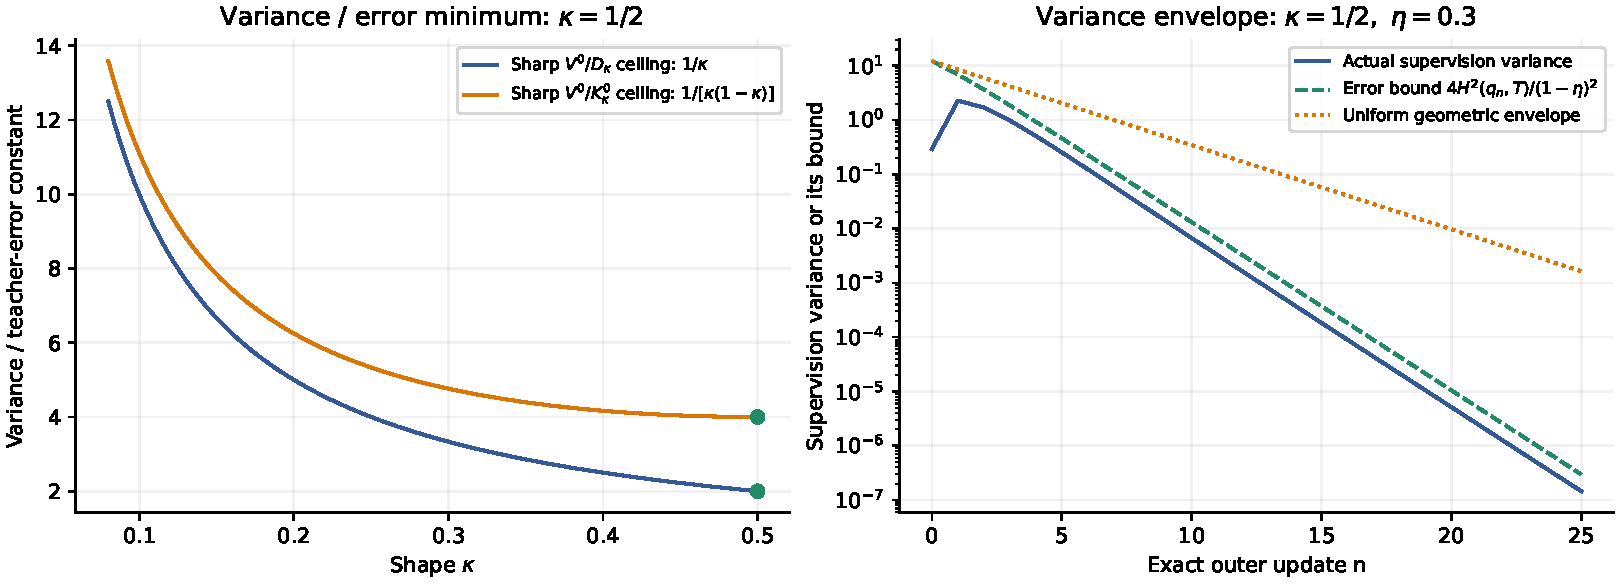
\includegraphics[width=\textwidth]{../../results/chapter9-restructure/relative-noise-and-convergence.pdf}
 \caption{左图展示相对教师误差的锐噪声常数在 $\kappa=1/2$ 处达到唯一最小值。右图展示对 $q_0=(0.999,0.001), t=(0.05,0.95), \eta=0.3$ 执行精确平方根外层迭代时，Hellinger 驱动的几何方差包络严格指数衰减。}
 \label{fig:power-relative-noise-convergence}
\end{figure}

\subsection{所有形状共享局部渐近收敛率与综合形状选择判据}

\begin{theorem}[幂均值族在教师邻域的二阶展开与共同局部收缩率 $(1-\eta)^2$]
\label{thm:power-common-local-rate}
固定严格正教师 $t$、$0<\eta<1$ 与 $0\le\kappa\le 1$。设锚点为局部扰动 $q=t+\epsilon h$（其中 $\sum_a h_a=0, h\ne 0, \epsilon\to 0$），记 $w=1-\eta$、Fisher 范数平方 $S_h=\sum_a h_a^2/t_a$。则幂均值目标满足二阶展开：
\begin{equation}
 m_a=t_a+w\epsilon h_a
 +\frac{(\kappa-1)w\eta}{2}\epsilon^2
       \left(\frac{h_a^2}{t_a}-t_a S_h\right)+O(\epsilon^3).
 \label{eq:power-second-order-target}
\end{equation}
对任意在 $1$ 附近三阶可微且 $g''(1)>0$ 的凸生成函数 $g$，单步散度比值恒为
\begin{equation}
 \frac{D_g(m\Vert t)}{D_g(q\Vert t)}
 =(1-\eta)^2+O(\epsilon).
 \label{eq:power-local-divergence-rate}
\end{equation}
\end{theorem}
\begin{proof}
对 $[(1-\eta)(t_a+\epsilon h_a)^\kappa+\eta t_a^\kappa]^{1/\kappa}$ 做二阶泰勒展开得未归一化权重 $\widetilde m_a=t_a+w\epsilon h_a+\frac{(\kappa-1)w\eta}{2}\epsilon^2(h_a^2/t_a)+O(\epsilon^3)$，求和得配分函数 $Z=1+\frac{(\kappa-1)w\eta}{2}\epsilon^2 S_h+O(\epsilon^3)$，相除即得式~\eqref{eq:power-second-order-target}。由于一阶项 $w\epsilon h_a=(1-\eta)(q_a-t_a)$ 与形状 $\kappa$ 完全无关，代入二阶局部 Fisher 展开 $D_g(p\Vert t)=\frac12 g''(1)\sum_a(p_a-t_a)^2/t_a+O(\epsilon^3)$ 相除即得共同局部收缩因子 $(1-\eta)^2$。
\end{proof}

\begin{figure}[H]
 \centering
 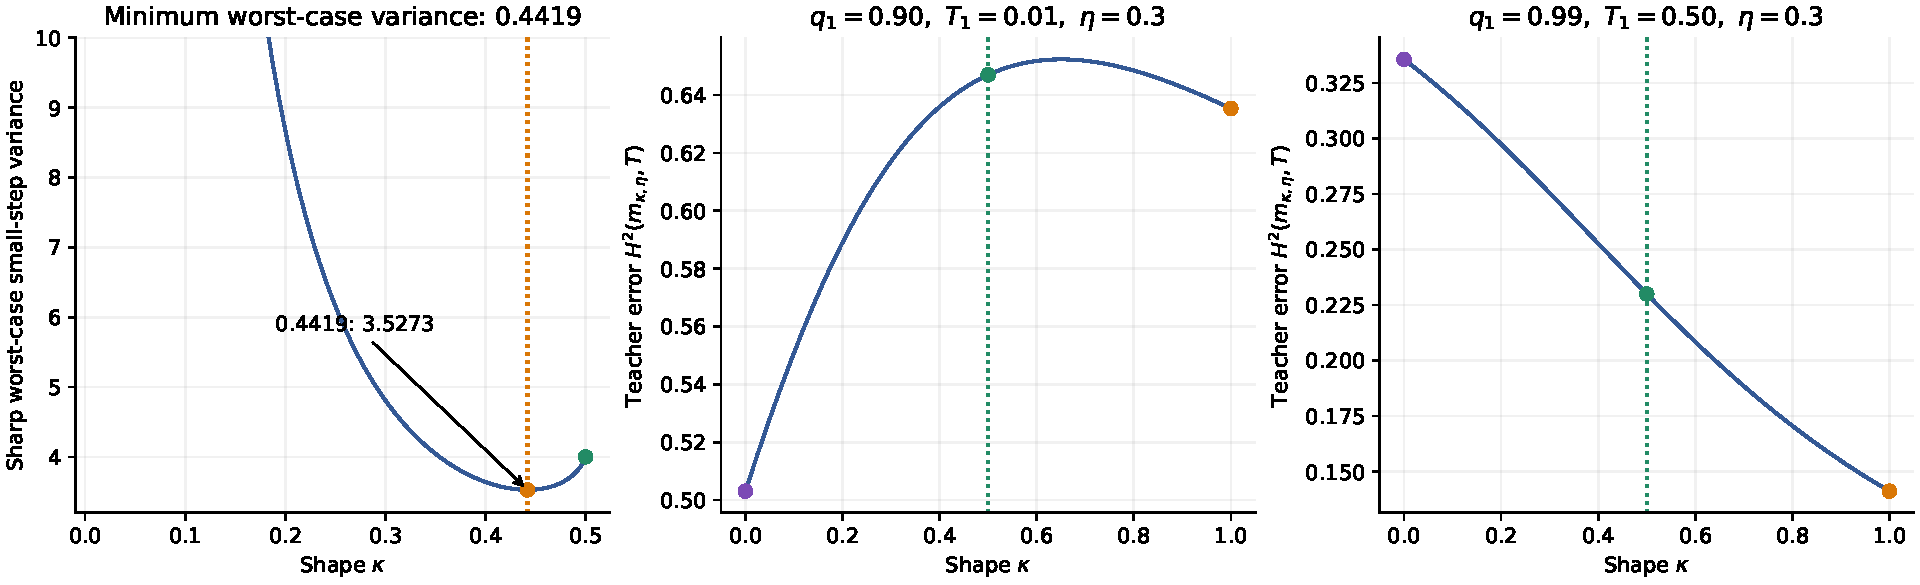
\includegraphics[width=\textwidth]{../../results/chapter9-restructure/kappa-criteria.pdf}
 \caption{不同评价准则下的形状参数表现。左图为最坏小步方差锐常数 $C_{\mathrm{vel}}(\kappa)$；中、右图展示在同一 $\eta=0.3$ 下，针对两对不同的固定二元分布 $(q,t)$，单步精确更新后的 Hellinger 误差关于 $\kappa$ 呈现相反的单调趋势。}
 \label{fig:power-kappa-criteria}
\end{figure}

\begin{center}
\small
\begin{tabular}{p{55mm}p{35mm}p{54mm}}
\toprule
理论评价准则 & 最优形状参数 $\kappa$ & 数学条件与物理含义\\
\midrule
小步监督具有分布无关有限二阶矩 & $0<\kappa\le 1/2$ & $\kappa=1/2$ 是该有界方差区间的最大形状端点\\
小步方差相对于教师散度误差的最坏比值 & $\kappa=1/2$（唯一最小） & $V\le 2D_{1/2}=4H^2$，相对误差噪声放大系数最小\\
小步绝对标量方差／自然梯度速度上确界 & $\kappa_\star\approx 0.441928$ & 锐极小极大值 $3.527275$（平方根点 $\kappa=1/2$ 为 $4$）\\
固定 Fisher 步幅下逆向 KL $\KL(q\Vert t)$ 最速下降 & $\kappa=0$（几何插值） & 确定性一阶下降最陡，但负尾部无界、无统一方差界\\
固定 Fisher 步幅下正向 KL $\KL(t\Vert q)$ 最速下降 & $\kappa=1$（算术混合） & 确定性一阶下降最陡，但小步最坏方差按 $\Theta(\eta^{-1})$ 发散\\
当前学生采样下幂散度拟合的自界噪声常数 & $\kappa_{\mathrm{fit}}=1/2$ & 梯度二阶矩与拟合损失之比达到最小锐常数 $1/\kappa_{\mathrm{fit}}=2$\\
固定 $(q,\eta)$ 下独立 Logits 的 BPO 条件数 & 对所有 $\kappa\in[0,1]$ 相同 & $\nabla_z^2\mathcal L_{\mathrm{BPO}}=F_q/\eta$，形状仅改变目标位置与起始残差\\
教师邻域的局部一阶散度渐近收缩率 & 对所有 $\kappa\in[0,1]$ 相同 & 局部渐近比值恒为 $(1-\eta)^2$（式~\eqref{eq:power-local-divergence-rate}）\\
\bottomrule
\end{tabular}
\end{center}

\section{高维概率路径、Escort 线性轨迹与自界拟合目标}
\label{sec:power-projection}

\subsection{精确幂均值外层步降低全体凸 \texorpdfstring{$f$}{f}-散度、保序 Markov 核与目标半径单调性}

\begin{theorem}[精确幂均值目标步的全局全 $f$-散度单调性与目标半径单调性]
\label{thm:proximal-all-f-divergences}
\label{thm:power-target-radius}
固定严格正分布 $q,t\in\Delta_V^\circ$、$\kappa\in[0,1]$ 与 $0<\eta<1$。对任意满足 $\varphi(1)=0$ 的凸生成函数 $\varphi:(0,\infty)\to\R$：
\begin{enumerate}
\item \textbf{到教师的全 $f$-散度单调下降}：精确幂均值目标 $m=m_{\kappa,\eta}(q,t)$ 恒满足 $D_\varphi(m\Vert t)\le D_\varphi(q\Vert t)$，且存在一个以教师 $t$ 为平稳分布（$t\mathsf P=t$）并满足细致平衡条件的可逆 Markov 转移矩阵 $\mathsf P$，使得 $q\mathsf P=m$。
\item \textbf{到锚点的目标位移半径随 $\eta$ 严格递增}：散度半径 $D_\varphi(m_{\kappa,\eta}\Vert q)$ 关于插值强度 $\eta\in[0,1]$ 单调非减；当 $q\ne t$ 且 $\varphi$ 严格凸时，在 $\eta\in(0,1)$ 上严格递增。
\end{enumerate}
\end{theorem}
\begin{proof}
第一条既可作为定理~\ref{thm:power-bpo-inner-all-f} 在端点 $\xi=1$ 的特例，也可由共单调性直接证明：令 $s_a=q_a/t_a$，$G(s)=[(1-\eta)s^\kappa+\eta]^{1/\kappa}$，则 $m_a/t_a=G(s_a)/Z$。因 $G(s)$ 递增且 $G(s)/s$ 递减，存在唯一交点 $s_\star$ 使 $G(s_\star)/s_\star=Z$，且每个比率 $s_a'=G(s_a)/Z$ 均被压缩在 $s_a$ 与 $s_\star$ 之间，故对任意 $c\in\partial\varphi(s_\star)$ 有 $\varphi(s_a')-c s_a'\le\varphi(s_a)-c s_a$，关于 $t$ 求和即得 $D_\varphi(m\Vert t)\le D_\varphi(q\Vert t)$。令 $\delta=m-q$，$L=\{a:\delta_a>0\}, H=\{b:\delta_b<0\}, D=\sum_{a\in L}\delta_a$，构造转移矩阵非对角元 $\mathsf P_{ab}=\frac{\delta_a(-\delta_b)}{D T_a(s_b-s_a)}$（$a\in L, b\in H$），直接验证即满足细致平衡 $t_a\mathsf P_{ab}=t_b\mathsf P_{ba}$ 及 $q\mathsf P=m$。第二条同理：对 $0<\eta_1<\eta_2<1$，比值 $m_{\eta_2,a}/m_{\eta_1,a}$ 关于 $\rho_a=t_a/q_a$ 严格递增，使得 $m_{\eta_2,a}/q_a$ 相对于 $m_{\eta_1,a}/q_a$ 向唯一交点两侧向外扩张，由凸函数保序性即得 $D_\varphi(m_{\eta_2}\Vert q)\ge D_\varphi(m_{\eta_1}\Vert q)$。
\end{proof}

\paragraph{有限内层拟合下的逆向 KL 与 R\'enyi 进展证书。}
当内层学生 $p$ 仅近似拟合 $m$ 时，记拟合误差为 $\epsilon=\KL(p\Vert m)$，对数比率 $\ell_T(a)=\log(m_a/t_a)$，跨度 $H=\operatorname{osc}(\ell_T)$。由 Pinsker 不等式与变分对偶（引入 $r_u(a)=m_a^{1+u}t_a^{-u}/C_u,\; C_u=\sum_a m_a^{1+u}t_a^{-u}$），当前学生的真实教师逆向 KL 同时满足区间证书与 R\'enyi 散度证书：
\begin{align}
 \KL(p\Vert t)&\le\KL(m\Vert t)+\epsilon+H\sqrt{\frac{\epsilon}{2}},
 \label{eq:proximal-range-certificate}\\
 \boxed{\KL(p\Vert t)\le
 \inf_{u>0}\left[\left(1+\frac1u\right)\KL(p\Vert m)+D_{1+u}^{\mathrm R}(m\Vert t)\right]},\qquad
 D_{1+u}^{\mathrm R}(m\Vert t)=\frac1u\log C_u.
 \label{eq:proximal-renyi-certificate}
\end{align}

\subsection{重心散度进展恒等式与 Escort 坐标下的精确线性轨迹}

\begin{theorem}[教师幂散度的有限内层进展恒等式]
\label{thm:proximal-teacher-progress}
记 $c_\kappa=Z^\kappa$（端点 $\kappa=0,1$ 取 $c_\kappa=1$）。对任意候选学生分布 $p\in\Delta_V^\circ$，恒成立三点分解：
\begin{equation}
 \eta\bigl[D_\kappa(t\Vert q)-D_\kappa(t\Vert p)\bigr]
 =(1-\eta)D_\kappa(q\Vert p)
 +c_\kappa\bigl[D_\kappa(m\Vert q)-D_\kappa(m\Vert p)\bigr].
 \label{eq:proximal-progress-identity}
\end{equation}
因此，只要内层更新使目标幂散度不劣于起点（即 $D_\kappa(m\Vert p)\le D_\kappa(m\Vert q)$），外层教师幂散度 $D_\kappa(t\Vert p)$ 就必然单调下降。
\end{theorem}
\begin{proof}
由重心定义 $F(q)=\eta D_\kappa(t\Vert q)$ 与 $F(p)=(1-\eta)D_\kappa(q\Vert p)+\eta D_\kappa(t\Vert p)$，相减并代入定理~\ref{thm:proximal-barycenter-gap} 的超额损失恒等式 $F(q)-F(p)=c_\kappa[D_\kappa(m\Vert q)-D_\kappa(m\Vert p)]$ 移项即得。
\end{proof}

对任意正形状 $0<\kappa\le 1$，定义单纯形上的 \textbf{Escort 变换（幂归一化映射）} 与幂和：
\begin{equation}
 E_\kappa(q)_a=\frac{q_a^\kappa}{S_\kappa(q)},\qquad
 S_\kappa(q)=\sum_{b\in\mathcal V} q_b^\kappa.
\end{equation}
$E_\kappa:\Delta_V^\circ\to\Delta_V^\circ$ 是光滑双射（逆映射为 $q_a\propto E_\kappa(q)_a^{1/\kappa}$）。由于 $m_a^\kappa=[(1-\eta)q_a^\kappa+\eta t_a^\kappa]/Z^\kappa$，公共配分常数在 Escort 归一化中精确相消，使得非线性幂均值更新在 Escort 坐标下化为\textbf{精确凸组合直线段}！
\begin{equation}
 E_\kappa(m)=(1-a^{\mathrm{esc}})E_\kappa(q)+a^{\mathrm{esc}}E_\kappa(t),\qquad
 a^{\mathrm{esc}}=\frac{\eta S_\kappa(t)}{(1-\eta)S_\kappa(q)+\eta S_\kappa(t)}\in(0,1).
 \label{eq:proximal-escort-step}
\end{equation}
当外层反复执行 $q_{k+1}=m_{\kappa,\eta}(q_k,t)$ 时，记 $e_k=E_\kappa(q_k), e_t=E_\kappa(t)$，则 $V-1$ 维非线性轨迹精确共线且坍缩为单标量乘积：
\begin{equation}
 e_k-e_t=b_k(e_0-e_t),\qquad
 b_k=\prod_{j=0}^{k-1}\bigl(1-a_j^{\mathrm{esc}}\bigr).
 \label{eq:proximal-escort-orbit}
\end{equation}
同样地，连续自然梯度流 $\frac{dq_a}{d\tau_{\mathrm{flow}}}=q_a(\rho_a^\kappa-a_\kappa)/\kappa$ 在 Escort 坐标下满足 $\frac{d}{d\tau_{\mathrm{flow}}}E_\kappa(q)=\frac{S_\kappa(t)}{S_\kappa(q)}[E_\kappa(t)-E_\kappa(q)]$，离散幂均值步与连续自然梯度流共享完全相同的几何轨迹（仅作时间重参数化）。

\begin{figure}[htbp]
 \centering
 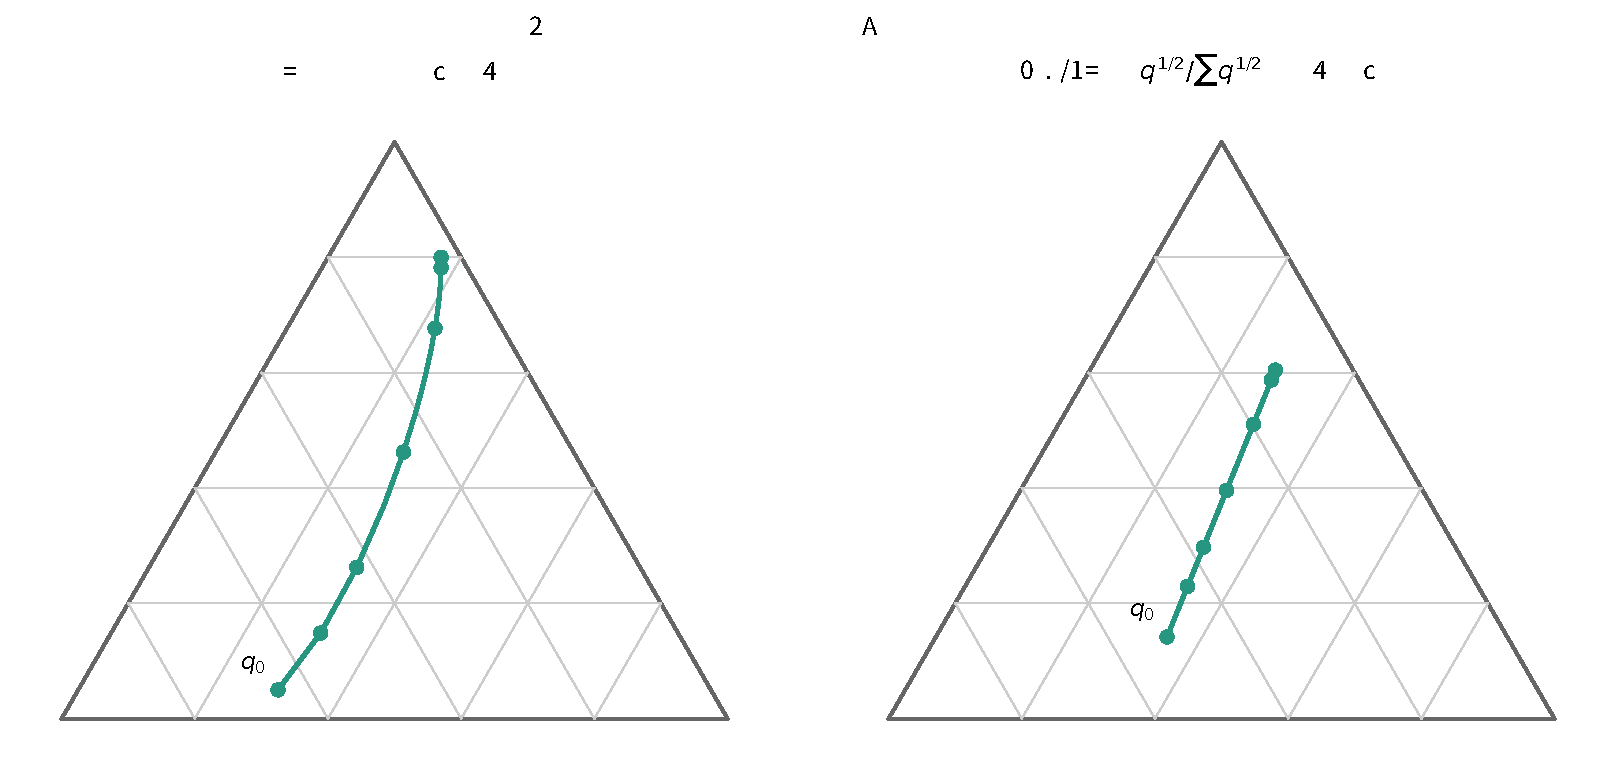
\includegraphics[width=\textwidth]{../../results/proximal-family-geometry/escort.pdf}
 \caption{同一条平方根（$\kappa=1/2$）外层轨迹在原概率坐标中弯曲，而在 Escort 坐标 $E_{1/2}(q)$ 中是精确直线。}
\end{figure}

\begin{theorem}[Escort 度量下的定向几何收缩与扰动误差累积界]
\label{thm:proximal-escort-contraction}
设词表大小为 $V$，$0<\kappa\le 1$，定义 Escort 距离 $d_\kappa(q,t)=\|E_\kappa(q)-E_\kappa(t)\|_1$。则精确外层更新满足一致几何收缩：
\begin{equation}
 d_\kappa(q_{k+1},t)=\bigl(1-a_k^{\mathrm{esc}}\bigr)d_\kappa(q_k,t)\le c\,d_\kappa(q_k,t),\qquad
 c=\frac{(1-\eta)V^{1-\kappa}}{(1-\eta)V^{1-\kappa}+\eta S_\kappa(t)}<1.
\end{equation}
若有限内层近似更新满足 $d_\kappa(q_{k+1},m(q_k,t))\le\epsilon_k$（且 $\limsup_{k\to\infty}\epsilon_k\le\epsilon_\infty$），则
\begin{equation}
 d_\kappa(q_k,t)\le c^k d_\kappa(q_0,t)+\sum_{j=0}^{k-1}c^{k-1-j}\epsilon_j,
 \qquad
 \limsup_{k\to\infty}d_\kappa(q_k,t)\le\frac{\epsilon_\infty}{1-c}.
\end{equation}
\end{theorem}
\begin{proof}
由 Hölder/Jensen 不等式知 $S_\kappa(q)=\sum_a q_a^\kappa\le V^{1-\kappa}$，故 $1-a_k^{\mathrm{esc}}\le c<1$。结合式~\eqref{eq:proximal-escort-step} 与三角不等式展开递推即得。
\end{proof}

\begin{figure}[htbp]
 \centering
 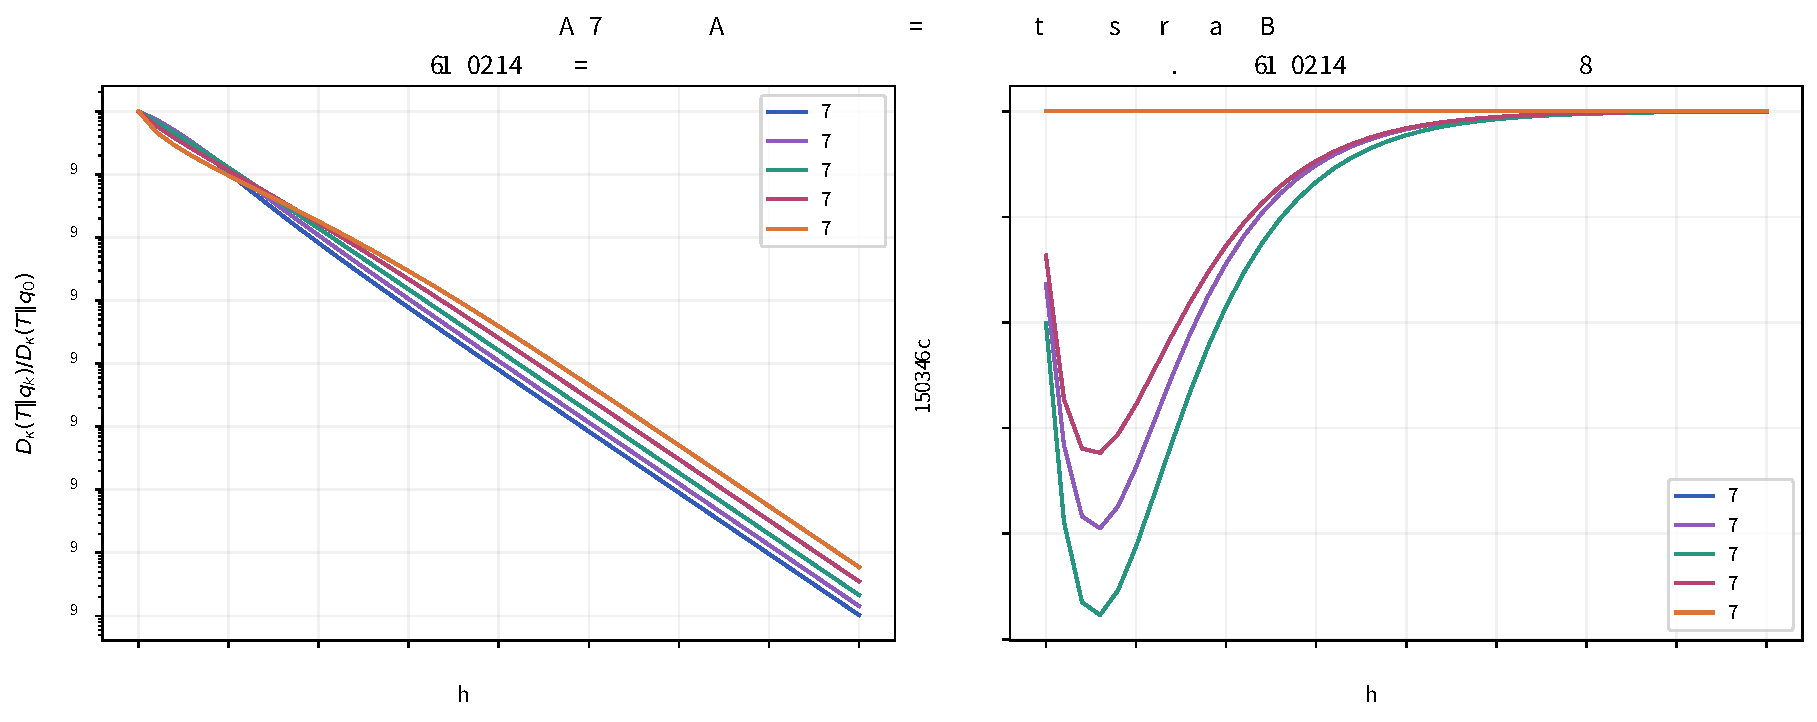
\includegraphics[width=\textwidth]{../../results/proximal-family-geometry/convergence.pdf}
 \caption{精确外层迭代下各形状教师散度单调下降，且有效 Escort 步幅 $a_k^{\mathrm{esc}}$ 在趋近教师时收敛于共同的 $\eta$。}
\end{figure}

\subsection{当前学生采样下的自界拟合目标与条件 SGD 收敛定理}

如果将“构造目标 $m$ 的形状 $\kappa_{\mathrm{target}}$”与“内层拟合 $m$ 的散度形状 $\kappa_{\mathrm{fit}}$”解耦：固定 $m$ 后，从当前学生 $a\sim p$ 采样动作，直接最小化 $D_{\kappa_{\mathrm{fit}}}(m\Vert p)$。记 $k=\kappa_{\mathrm{fit}}$、$\chi_a=m_a/p_a$、$a_k=\E_p[\chi^k]$，解析梯度的无偏单样本估计量为 $g_k(a)=\frac{a_k-\chi_a^k}{k}\psi_p(a)$。

\begin{theorem}[当前学生采样下误差相关梯度二阶矩的锐常数与条件 SGD 收敛]
\label{thm:proximal-sharp-self-bound}
\label{thm:power-conditional-sgd}
\begin{enumerate}
\item \textbf{自界噪声锐常数}：若 $\|\psi_p(a)\|\le S$ 且 $0<\kappa_{\mathrm{fit}}\le 1/2$，则单样本梯度二阶矩与当前拟合散度成正比：
\begin{equation}
 \Var_p(g_{\kappa_{\mathrm{fit}}})\le\E_p\|g_{\kappa_{\mathrm{fit}}}\|^2
 \le\frac{S^2}{\kappa_{\mathrm{fit}}}D_{\kappa_{\mathrm{fit}}}(m\Vert p).
\end{equation}
系数 $1/\kappa_{\mathrm{fit}}$ 是完整支持分布类上的锐常数，在 $\kappa_{\mathrm{fit}}=1/2$（Hellinger 拟合）处取得唯一最小值 $2$（而 $\kappa_{\mathrm{fit}}=0$ 或 $>1/2$ 无有限统一常数）。
\item \textbf{误差相关噪声下的条件 SGD 线性收敛}：对满足 $L_{\mathrm{sm}}$-光滑、$\mu$-PL 条件 $\|\nabla L\|^2\ge 2\mu(L-L_\star)$ 且随机梯度无偏并满足自界二阶矩 $\E[\|g\|^2\mid\theta]\le C L(\theta)$ 的内层目标（精确完整中心 BPO 同样满足该条件，$C=2S^2/\eta$），取步长 $0<\alpha_{\mathrm{opt}}\le\min\{1/\mu, 2\mu/(L_{\mathrm{sm}}C)\}$，记 $c_{\mathrm{SGD}}=1-\mu\alpha_{\mathrm{opt}}\in[0,1)$，则 $N$ 步内层迭代满足
\begin{equation}
 \E\bigl[L(\theta_N)-L_\star\bigr]
 \le c_{\mathrm{SGD}}^N\bigl[L(\theta_0)-L_\star\bigr]
 +\frac{L_{\mathrm{sm}}C\alpha_{\mathrm{opt}}L_\star}{2\mu}\bigl(1-c_{\mathrm{SGD}}^N\bigr).
\end{equation}
特别地，当目标可实现（$L_\star=0$）时，无需缩减学习率即可消除稳态采样噪声底，以几何速率收敛至零损失。
\end{enumerate}
\end{theorem}
\begin{proof}
第一条与定理~\ref{thm:power-relative-noise-optimum} 完全对称（将参考测度换为 $p$、比率换为 $\chi=m/p$）。第二条由 $L_{\mathrm{sm}}$-光滑展开 $\E[L(\theta^+)\mid\theta]\le L-\alpha_{\mathrm{opt}}\|\nabla L\|^2+\frac12 L_{\mathrm{sm}}\alpha_{\mathrm{opt}}^2 C L$，代入 PL 条件并将 $L=(L-L_\star)+L_\star$ 拆分，利用 $\frac12 L_{\mathrm{sm}}C\alpha_{\mathrm{opt}}^2\le\mu\alpha_{\mathrm{opt}}$ 归纳即得。
\end{proof}

\begin{figure}[htbp]
 \centering
 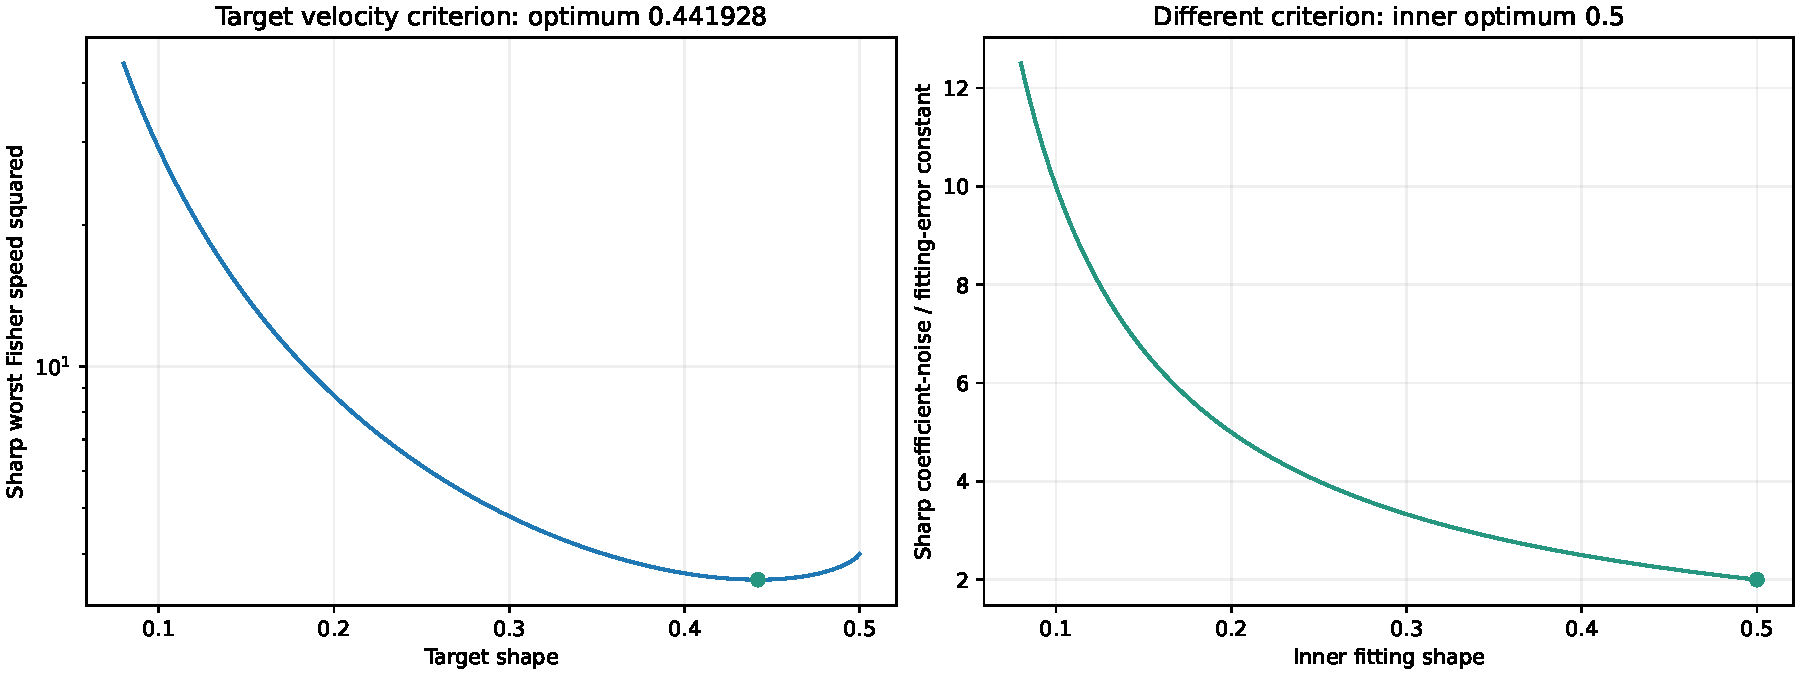
\includegraphics[width=\textwidth]{../../results/power-mean-20261013/two-minimax-criteria.pdf}
 \caption{两个不同的极小极大形状准则对比。左图是目标自然梯度速度的锐上界 $C_{\mathrm{vel}}(\kappa)$（最小点 $\kappa_\star\approx 0.441928$）；右图是内层拟合目标的误差相关噪声锐常数 $1/\kappa_{\mathrm{fit}}$（最小点 $\kappa_{\mathrm{fit}}=1/2$）。}
\end{figure}

\subsection{幂均值框架可用理论性质总结与标准化反例}

我们将第一篇建立的单教师幂均值 MirrorOPD 可用性质及前提条件总结如下表：

\begin{center}
\small
\begin{tabular}{>{\raggedright\arraybackslash}p{46mm}>{\raggedright\arraybackslash}p{54mm}>{\raggedright\arraybackslash}p{45mm}}
\toprule
可用理论性质 & 严格数学前提条件 & 工程与算法含义\\
\midrule
精确目标步同时改善全体凸 $f$-散度 & 同一固定教师 $t$、完整正支持 & 同一评价散度下可跨形状公平比较\\
教师覆盖与刷新后双侧有界监督 & $\kappa>0$，同一前缀精确刷新 & $q_k\ge\eta^{1/\kappa}t$，自动控制后续轮次正尾部\\
精确 MD 单步下降与末步 $O(1/(\eta K_{\mathrm{out}}))$ 界 & 固定 $(\kappa,\eta)$，每轮刷新锚点 & $\mathcal J(q_{K_{\mathrm{out}}};t)\le\KL(t\Vert q_0)/(\eta K_{\mathrm{out}})$\\
教师监督方差受误差控制且全轮可求和 & $0<\kappa\le 1/2$，精确外层刷新 & 教师接近度与初始监督噪声同步趋零\\
BPO 零残差处采样梯度精确归零 & 目标可实现、精确中心或成对差分损失 & 消除固定教师中心误差造成的末期噪声底\\
有限内层步的全 $f$-散度单调进展 & 从 $q$ 出发的锚点 Fisher 预条件路径 & 任意降低 BPO 损失的更新步不自动保单调\\
\bottomrule
\end{tabular}
\end{center}

\paragraph{注记（条件标准差归一化会抵消形状变换的方差缩减效应）。}
在二元分布 $q=(v,1-v)$ 下，对任意非恒定信号 $f$（$f_1\ne f_2$），其条件方差为 $\sigma_f^2=v(1-v)(f_1-f_2)^2$。若将中心化信号除以条件标准差 $\sigma_f$，则逐动作展开立得 $\Var_q[\psi_q C_q f/\sigma_f]=(1-2v)^2$，完全消去了非线性信号变换 $f_{\kappa,\eta}$ 的作用！因此幂均值 MirrorOPD 严格只做加性中心化 $C_q A_{\kappa,\eta}$，绝不除以随机或条件标准差。

\begin{figure}[htbp]
 \centering
 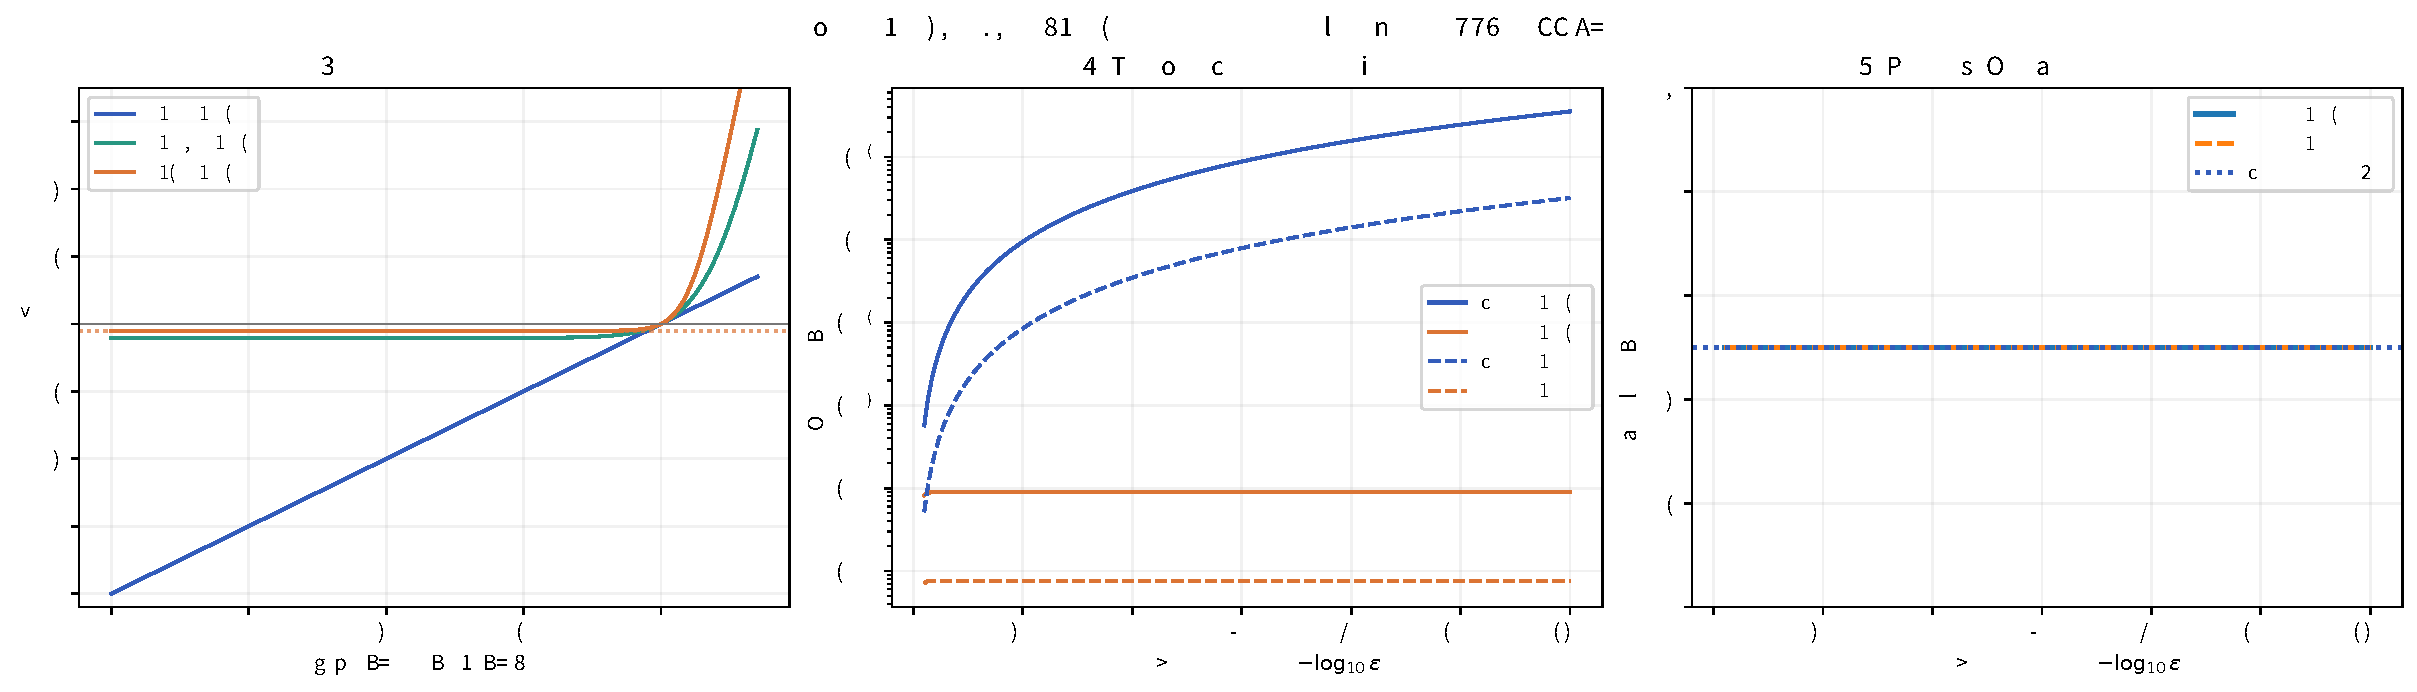
\includegraphics[width=\textwidth]{../../results/proximal-family-geometry/variance.pdf}
 \caption{尺度、尾部饱和与标准差归一化分别改变不同统计量。左图展示 $\eta$（图中旧记号 $\lambda$）缩放；中图展示固定 $q=(1/4,3/4)$ 下的条件中心化得分方差；右图验证二元标准差归一化抵消形状变换的现象。}
\end{figure}

\part{OPD 实例化、信息访问与条件积分估计}

\chapter{信息访问、KL 分区粗化与条件随机积分估计}
\label{inf:chapter}
\label{est:chapter}

第一篇建立了固定前缀测度下的四种内层投影目标、同步动力学与幂均值广义重心理论。然而，在实际语言模型蒸馏系统中，能否精确或无偏地计算这些目标，取决于教师与锚点模型的\textbf{信息查询接口（Query Interface）}。完整词表 Logits、稀疏 Top-$J$ 头部加尾部桶质量、以及实际采样动作的对数概率提供截然不同的信息量。

本章将信息可识别性理论、条件随机积分残差控制框架、自动微分（Autodiff）向量场分析以及幂均值中心与无重复成对动作估计整合为统一的估计理论。全书的锚点、学生、教师仍分别记为 $q,p,t$；本章在分析一般条件 KL 估计时使用占位学生分布 $P=P_\theta$ 与冻结参考分布 $Q$（分析 On-Policy OPD 时取 $P=p,Q=t$；分析学生--锚点 KL 时取 $P=p,Q=q$；实际动作采样分布记为 $\beta$，$A\sim\beta$）。默认有限词表上 $P(v),Q(v)>0$，定义
\begin{equation}
\ell_v=\ell_v^{P,Q}=\log\frac{P(v)}{Q(v)},\qquad
\psi_v=\nabla_\theta\log P(v),\qquad
\sg(\cdot)=\operatorname{stopgrad}(\cdot).
\end{equation}
对积分权重测度 $\mu$ 定义 $I_\mu(h)=\sum_{v\in\mathcal V}\mu(v)h_v=\E_\mu[h]$。记逆向与正向 KL 为 $K=\KL(P\Vert Q)$、$K^{\mathrm F}=\KL(Q\Vert P)$。由归一化恒等式 $\sum_v P(v)\psi_v=\nabla_\theta\sum_v P(v)=0$，逐项求导得到四个基本积分对象：
\begin{align}
g=\nabla_\theta K
&=\sum_v\bigl[(\nabla_\theta P(v))\ell_v+P(v)\nabla_\theta\ell_v\bigr]
=\sum_v P(v)(\ell_v+1)\psi_v
=I_P(\ell\psi),\\
g^{\mathrm F}=\nabla_\theta K^{\mathrm F}
&=-\sum_v Q(v)\nabla_\theta\ell_v=-I_Q(\psi).
\end{align}
向量估计量 $\widehat I$ 的方差统一定义为协方差矩阵之迹：
\begin{equation}
\operatorname{Bias}(\widehat I)=\E_\beta[\widehat I]-I_\nu(h),\qquad
\operatorname{MSE}(\widehat I)=\|\operatorname{Bias}(\widehat I)\|^2+\operatorname{tr}\operatorname{Cov}_\beta(\widehat I).
\end{equation}

\section{查询接口及其可识别信息类}
\label{inf:access}
\label{est:targets}

固定前缀 $s$。完整 Logits 接口给出整个 $t(\cdot\mid s)$，所有有限词表求和均可精确计算。稀疏 Top-$J$ 接口给出冻结头部支持集 $S$（$|S|=J$）及每个 $v\in S$ 的 $t(v\mid s)$；由概率归一化可精确获知尾部总质量 $\tau_t=1-\sum_{v\in S}t(v\mid s)$，但通常无法恢复每个尾部动作的单独概率。实际采样动作查询给出已抽取动作 $A$ 处的 $t(A\mid s)$，提供一个新的坐标点观测。

\begin{definition}[与观测一致的兼容参考分布类]
\label{inf:compatible}
设词表分区为 $\mathcal C$，已知各桶总质量 $Q_C>0$（$\sum_{C\in\mathcal C}Q_C=1$）。仅使用桶质量观测时，兼容参考分布的信息类定义为
\begin{equation}
\mathfrak Q_{\mathcal C}=\left\{\widetilde Q\in\Delta_V^\circ:\;\widetilde Q(v)>0,\quad \sum_{v\in C}\widetilde Q(v)=Q_C\text{ 对每个 }C\in\mathcal C\right\}.
\end{equation}
若同时观测到动作集合 $O$ 上的精确概率，则加入点约束 $\widetilde Q(v)=Q(v)$（$\forall v\in O$）。若已知 $S$ 是真实参考分布的 Top-$J$ 集合，还加入排名上界约束：
\begin{equation}
\widetilde Q(v)\leq\min_{u\in S}Q(u),\qquad \forall v\notin S.
\end{equation}
一个目标量可由当前查询接口唯一识别，当且仅当它在相应兼容信息类上恒取相同值。
\end{definition}

四种内层方法所需的确定性积分对象及更新时点汇总如下：
\begin{center}
\begin{tabular}{lll}
\toprule
内层方法 & 所需条件积分或点查询对象 & 外层冻结或内层重算\\
\midrule
PMD-Part & $\log Z_f=\log\E_q[e^{\eta f}]$ & 整轮外层冻结\\
PMD-Mean & $\E_q[f]$ & 整轮外层冻结\\
BPO（中心表示） & $\E_q[f],\;\E_q[U],\;\E_q[\psi]$ & 教师信号冻结，学生项每步重算\\
BPO（成对差分表示） & $U_a-U_b,\; f_a-f_b$ & 仅需两个动作点上的函数值\\
MDPO & $\E_p[(U/\eta-f)\psi]$ & 学生测度权重随内层每步重算\\
\bottomrule
\end{tabular}
\end{center}

\section{词表分区上的 KL 粗化、梯度残差与可识别性边界}
\label{inf:sec:kl-partition-geometry}
\label{inf:sec:kl-partition}
\label{inf:identification}

\begin{definition}[词表分区与桶内条件分布]
令 $\mathcal C$ 是有限词表 $\mathcal V$ 的一个固定分区，各单元 $C\in\mathcal C$ 非空且两两不交，$\bigcup_{C\in\mathcal C}C=\mathcal V$。定义桶质量与桶对数概率比：
\begin{equation*}
 P_C=\sum_{v\in C}P(v),\qquad
 Q_C=\sum_{v\in C}Q(v),\qquad
 \ell_C=\log\frac{P_C}{Q_C},
\end{equation*}
以及桶内条件分布和桶平均学生得分向量：
\begin{equation*}
 P^C(v)=\frac{P(v)}{P_C},\qquad
 Q^C(v)=\frac{Q(v)}{Q_C},\qquad
 \bar \psi_C=\sum_{v\in C}P^C(v)\psi_v=\nabla_\theta\log P_C.
\end{equation*}
用 $C(v)$ 表示包含动作 $v$ 的唯一分区单元。粗粒度 $\KL(P\Vert Q)$ 与桶内形状条件 KL 分别定义为
\begin{equation*}
 K_{\mathcal C}=\sum_{C\in\mathcal C}P_C\ell_C,
 \qquad D_C=\KL(P^C\Vert Q^C).
\end{equation*}
\end{definition}

\begin{theorem}[同一词表分区上的双向 KL 链式分解]
\label{inf:thm:kl-partition-chain}
在正支持假设下，$\KL(P\Vert Q)$ 和 $\KL(Q\Vert P)$ 分别满足精确分解：
\begin{align}
 K&=K_{\mathcal C}+\sum_{C\in\mathcal C}P_C D_C,
 \label{inf:eq:kl-partition-chain-reverse}\\
 K^{\mathrm F}&=K^{\mathrm F}_{\mathcal C}
       +\sum_{C\in\mathcal C}Q_C D^{\mathrm F}_C,
 \label{inf:eq:kl-partition-chain-forward}
\end{align}
其中 $K^{\mathrm F}_{\mathcal C}=-\sum_C Q_C\ell_C$，$D_C^{\mathrm F}=\KL(Q^C\Vert P^C)$。因此两种方向的粗粒度 KL 都是对应完整 KL 的确定性下界，且等号成立当且仅当每个单元内的条件分布完全相同（$P^C=Q^C$）。
\end{theorem}
\begin{proof}
对任意 $v\in C$，完整对数概率比可逐点拆分为桶质量对数比与桶内条件对数比之和：
\begin{equation*}
 \ell_v=\log\frac{P(v)}{Q(v)}
     =\ell_C+\log\frac{P^C(v)}{Q^C(v)}.
\end{equation*}
先乘以 $P(v)=P_C P^C(v)$ 在单元 $C$ 内求和，再对所有单元 $C\in\mathcal C$ 求和，得到
\begin{equation*}
 \sum_v P(v)\ell_v
 =\sum_C P_C\ell_C
  +\sum_C P_C\sum_{v\in C}P^C(v)
                        \log\frac{P^C(v)}{Q^C(v)},
\end{equation*}
即得逆向分解式~\eqref{inf:eq:kl-partition-chain-reverse}。将逐点恒等式取负并乘以 $Q(v)=Q_C Q^C(v)$ 求和，即得正向分解式~\eqref{inf:eq:kl-partition-chain-forward}。所有桶质量严格为正且条件 KL 非负，等号当且仅当每个 $D_C=0$（即 $P^C=Q^C$）时成立。
\end{proof}

\begin{proposition}[分区细化的标量单调性]
\label{inf:prop:kl-partition-refinement}
设分区 $\mathcal C'$ 细化分区 $\mathcal C$，记 $\mathcal C'|_C$ 为包含在 $C$ 内的细单元集合，则
\begin{equation*}
 K_{\mathcal C'}-K_{\mathcal C}
 =\sum_{C\in\mathcal C}P_C
   \KL\left(
       \left(\frac{P_{C'}}{P_C}\right)_{C'\in\mathcal C'|_C}
       \middle\Vert
       \left(\frac{Q_{C'}}{Q_C}\right)_{C'\in\mathcal C'|_C}
      \right)\geq0.
\end{equation*}
因此分区细化使粗粒度 KL 的标量偏差绝对值 $|K-K_{\mathcal C}|$ 和平方偏差单调下降；当全部单元均为单点集（singleton）时偏差精确为零。
\end{proposition}
\begin{proof}
对每个 $C\in\mathcal C$，利用 $\sum_{C'\subseteq C}P_{C'}=P_C$，将细化增量写为
\begin{equation*}
 \sum_{C'\subseteq C}P_{C'}\log\frac{P_{C'}}{Q_{C'}}
    -P_C\log\frac{P_C}{Q_C}
 =P_C\sum_{C'\subseteq C}\frac{P_{C'}}{P_C}
       \log\frac{P_{C'}/P_C}{Q_{C'}/Q_C}\ge 0.
\end{equation*}
对 $C\in\mathcal C$ 求和即得结论。
\end{proof}

\begin{theorem}[粗粒度 KL 的真实梯度及其协方差残差分解]
\label{inf:thm:kl-partition-gradient}
记粗粒度逆向 KL 的真实梯度为 $g_{\mathcal C}=\nabla_\theta K_{\mathcal C}$。则
\begin{align}
 g_{\mathcal C}
 &=\sum_{C\in\mathcal C}P_C\ell_C\bar \psi_C
  =\sum_{v\in\mathcal V}P(v)\ell_{C(v)}\psi_v,
 \label{inf:eq:kl-partition-gradient}\\
 g-g_{\mathcal C}
 &=\sum_{C\in\mathcal C}P_C\E_{P^C}\bigl[(\ell_A-\ell_C)\psi_A\bigr]
 \label{inf:eq:kl-partition-gradient-residual}\\
 &=\sum_{C\in\mathcal C}P_C\Bigl\{
       \operatorname{Cov}_{P^C}(\ell_A-\ell_C,\psi_A)
       +D_C\bar \psi_C\Bigr\},
 \label{inf:eq:kl-partition-gradient-covariance}
\end{align}
其中标量与向量的协方差定义为 $\operatorname{Cov}_{P^C}(u_A,\psi_A)=\E_{P^C}[(u_A-\E_{P^C}u_A)(\psi_A-\bar \psi_C)]$。对正向粗粒度目标 $K_{\mathcal C}^{\mathrm F}$，真实梯度及残差则为
\begin{equation*}
 g^{\mathrm F}_{\mathcal C}=-\sum_{C\in\mathcal C}Q_C\bar \psi_C,
 \qquad
 g^{\mathrm F}-g^{\mathrm F}_{\mathcal C}
 =-\sum_{C\in\mathcal C}Q_C\bigl\{\E_{Q^C}[\psi_A]-\bar \psi_C\bigr\}.
\end{equation*}
\end{theorem}
\begin{proof}
由于参考分布 $Q$ 冻结，$\nabla_\theta Q_C=0$，而 $\nabla_\theta P_C=P_C\bar \psi_C$。逐项求导得到
\begin{align*}
 \nabla_\theta K_{\mathcal C}
 &=\sum_C\bigl\{\ell_C\nabla_\theta P_C+P_C\nabla_\theta\ell_C\bigr\}
 =\sum_C\ell_C\nabla_\theta P_C+\sum_C\nabla_\theta P_C
 =\sum_C P_C\ell_C\bar \psi_C,
\end{align*}
其中利用了 $\sum_C\nabla_\theta P_C=\nabla_\theta 1=0$。将 $P_C\bar \psi_C=\sum_{v\in C}P(v)\psi_v$ 代入即得式~\eqref{inf:eq:kl-partition-gradient}。与完整梯度 $g=\sum_v P(v)\ell_v\psi_v$ 相减得式~\eqref{inf:eq:kl-partition-gradient-residual}；再利用 $\E_{P^C}[\ell_A-\ell_C]=D_C$ 与协方差恒等式展开每个桶内期望即得式~\eqref{inf:eq:kl-partition-gradient-covariance}。
\end{proof}

\begin{theorem}[桶质量信息下的 KL 下包络可识别性]
\label{inf:lower-envelope}
设 $P(v)>0$ 且每个已知桶质量 $Q_C>0$。在定义~\ref{inf:compatible} 的纯桶质量兼容信息类 $\mathfrak Q_{\mathcal C}$ 上，双向完整 KL 的下确界恰为粗粒度 KL：
\begin{equation}
\inf_{\widetilde Q\in\mathfrak Q_{\mathcal C}}\KL(P\Vert\widetilde Q)
=\sum_{C\in\mathcal C}P_C\log\frac{P_C}{Q_C}=K_{\mathcal C},\qquad
\inf_{\widetilde Q\in\mathfrak Q_{\mathcal C}}\KL(\widetilde Q\Vert P)
=\sum_{C\in\mathcal C}Q_C\log\frac{Q_C}{P_C}=K_{\mathcal C}^{\mathrm F},
\end{equation}
且两者由唯一的桶内条件分布匹配解 $\widetilde Q^\star(v)=Q_C P^C(v)$（$v\in C$）同时达到。
\end{theorem}
\begin{proof}
由定理~\ref{inf:thm:kl-partition-chain} 的双向链式分解，$\KL(P\Vert\widetilde Q)=K_{\mathcal C}+\sum_C P_C\KL(P^C\Vert\widetilde Q^C)\ge K_{\mathcal C}$，且等号当且仅当对所有 $C\in\mathcal C$ 均有 $\widetilde Q^C=P^C$（即 $\widetilde Q(v)=Q_C P^C(v)$）时成立；正向 KL 完全同理。
\end{proof}

\begin{proposition}[相同稀疏观测不控制完整 $\KL(P\Vert Q)$ 的上界及 Plug-in 配分估计的 Jensen 偏差]
\label{inf:unbounded}
\label{inf:jensen}
\begin{enumerate}
\item \textbf{上界无界性}：存在具有完全相同 Top-1 观测载荷的正支持参考分布族，使 Tail-Aware KL 保持不变而完整 $\KL(P\Vert Q)\to+\infty$。例如取 $P=(0.4,0.2,0.4)$ 与 $Q_\varepsilon=(0.7,\varepsilon,0.3-\varepsilon)$（$0<\varepsilon<0.15$），所有 $Q_\varepsilon$ 的 Top-1 均为动作 $1$（概率 $0.7$、尾部总质量 $0.3$），但 $\KL(P\Vert Q_\varepsilon)=0.4\log\frac{0.4}{0.7}+0.2\log\frac{0.2}{\varepsilon}+0.4\log\frac{0.4}{0.3-\varepsilon}\to+\infty$（当 $\varepsilon\downarrow 0$）。
\item \textbf{Plug-in 对数配分函数的 Jensen 负偏差}：若正随机估计量 $\widehat Z>0$ 满足 $\E[\widehat Z]=Z$ 且 $\E|\log\widehat Z|<\infty$，则由 $\log z\le\log Z+(z-Z)/Z$ 取期望得 $\E[\log\widehat Z]\le\log Z$，且等号当且仅当 $\widehat Z$ 几乎处处为常数时成立。（注：若在 $|\mathcal V|=D$ 维词表上从已知正支持锚点独立抽样 $m\ge D$ 次，令样本覆盖全词表的事件为 $E$，其已知概率为 $c=\Pr_q(E)>0$，则分段估计器 $\widehat L=\mathbf1_E\frac{\log Z}{c}$ 满足 $\E[\widehat L]=\log Z$ 与 $\Var(\widehat L)=(c^{-1}-1)(\log Z)^2$，说明“不存在任何无偏对数配分估计器”的绝对化断言并不成立，但该精确覆盖构造具有指数级方差。）
\item \textbf{粗化与真正的 Rao--Blackwell 化}：在 $A\sim P$ 下，给定桶标签 $C(A)=C$ 时 $\ell_A$ 的真实条件期望为 $\E_P[\ell_A\mid C(A)=C]=\ell_C+D_C$。由于稀疏接口下桶内形状项 $D_C$ 未知，Tail-Aware 仅保留 $\ell_C$（有偏），而 HETS 保留头部加尾部单点修正（并非全条件期望投影），故 HETS 的方差升降需由残差二阶矩直接判定。
\end{enumerate}
\end{proposition}

\section{统一估计构造：精确积分加残差抽样}
\label{est:sec:kl-residual-framework}

\begin{definition}[可精确积分的近似代理函数与残差修正估计量]
\label{est:def:kl-residual-integral}
令 $\nu$ 为词表上的目标积分概率测度，$f:\mathcal V\to\mathbb R^d$ 为目标被积函数，选取积分 $I_\nu(a)=\sum_v\nu(v)a_v$ 可精确计算的近似函数 $a:\mathcal V\to\mathbb R^d$，定义残差 $R_v=f_v-a_v$（故 $I_\nu(f)=I_\nu(a)+I_\nu(R)$）。设采样动作 $A\sim\beta$ 满足残差支持条件 $\nu(v)\|R_v\|>0\implies\beta(v)>0$，定义主残差修正估计量：
\begin{equation}
 \widehat I_{\nu,\beta,a}(f)
 =I_\nu(a)+\frac{\nu(A)}{\beta(A)}R_A.
 \label{est:eq:kl-master-estimator}
\end{equation}
\end{definition}

\begin{theorem}[残差修正估计量的均值、协方差与均方误差]
\label{est:thm:kl-master-moments}
记残差真均值为 $m_R=I_\nu(R)$。在定义~\ref{est:def:kl-residual-integral} 的支持条件下，式~\eqref{est:eq:kl-master-estimator} 对 $I_\nu(f)$ 严格无偏，且协方差矩阵与迹方差（即均方误差 MSE）为：
\begin{align}
 \operatorname{Cov}\bigl(\widehat I_{\nu,\beta,a}(f)\bigr)
 &=\sum_{v:\beta(v)>0}\frac{\nu(v)^2}{\beta(v)}R_v R_v^\top-m_R m_R^\top,
 \label{est:eq:kl-master-cov}\\
 \Var\bigl(\widehat I_{\nu,\beta,a}(f)\bigr)
 &=\sum_{v:\beta(v)>0}\frac{\nu(v)^2}{\beta(v)}\lVert R_v\rVert^2-\lVert m_R\rVert^2.
 \label{est:eq:kl-master-trace}
\end{align}
对 $m$ 个独立同分布动作的样本均值，其协方差与均方误差分别为上式的 $1/m$。
\end{theorem}
\begin{proof}
支持条件保证 $\beta(v)=0$ 的动作必有 $\nu(v)R_v=0$，因此随机修正项 $Y=\frac{\nu(A)}{\beta(A)}R_A$ 的期望为
\begin{equation*}
 \E_\beta[Y]=\sum_{v:\beta(v)>0}\beta(v)\frac{\nu(v)}{\beta(v)}R_v=\sum_{v\in\mathcal V}\nu(v)R_v=m_R,
\end{equation*}
故 $\E_\beta[\widehat I]=I_\nu(a)+m_R=I_\nu(f)$。确定性积分项 $I_\nu(a)$ 不影响协方差，计算 $\E_\beta[YY^\top]=\sum_{v:\beta(v)>0}\frac{\nu(v)^2}{\beta(v)}R_v R_v^\top$ 并减去 $m_R m_R^\top$ 即得式~\eqref{est:eq:kl-master-cov}，取迹即得式~\eqref{est:eq:kl-master-trace}。
\end{proof}

\begin{theorem}[确定项误差、错误权重与缺失支持的三源统一偏差定理]
\label{est:thm:kl-master-bias}
令 $\mathcal D=\{v:\beta(v)>0\}$。若实际程序输出的确定积分项带有固定误差 $\delta\in\R^d$，且实际使用的采样权重 $\widetilde w(v)$ 偏离真实比率 $\nu(v)/\beta(v)$，即输出 $\widetilde I=I_\nu(a)+\delta+\widetilde w(A)R_A$，则其相对于 $I_\nu(f)$ 的总偏差精确分解为：
\begin{equation}
 b_I=\E_\beta[\widetilde I]-I_\nu(f)=\delta
 +\sum_{v\in\mathcal D}\bigl(\beta(v)\widetilde w(v)-\nu(v)\bigr)R_v
 -\sum_{v\notin\mathcal D}\nu(v)R_v.
 \label{est:eq:kl-master-bias}
\end{equation}
记 $\widetilde m_R=\sum_{v\in\mathcal D}\beta(v)\widetilde w(v)R_v$，则协方差与均方误差分别为
\begin{align}
 \operatorname{Cov}(\widetilde I)
 &=\sum_{v\in\mathcal D}\beta(v)\widetilde w(v)^2 R_v R_v^\top
 -\widetilde m_R\widetilde m_R^\top,\\
 \E_\beta\lVert\widetilde I-I_\nu(f)\rVert^2
 &=\operatorname{tr}\operatorname{Cov}(\widetilde I)+\lVert b_I\rVert^2.
 \label{est:eq:kl-master-mse}
\end{align}
\end{theorem}
\begin{proof}
将 $\E_\beta[\widetilde I]=I_\nu(a)+\delta+\sum_{v\in\mathcal D}\beta(v)\widetilde w(v)R_v$ 与 $I_\nu(f)=I_\nu(a)+\sum_{v\in\mathcal D}\nu(v)R_v+\sum_{v\notin\mathcal D}\nu(v)R_v$ 直接相减即得式~\eqref{est:eq:kl-master-bias}，展开中心化二阶矩即得式~\eqref{est:eq:kl-master-mse}。
\end{proof}

\begin{theorem}[已知积分控制基函数的 Gram 矩阵最优组合与超额方差遗憾]
\label{est:thm:kl-master-gram}
设代理函数为线性组合 $a_{c,v}=\sum_{j=1}^{D_{\mathrm{ctrl}}}c_j h_{j,v}$，其中每个基函数积分 $I_\nu(h_j)$ 已知。记 $w(v)=\nu(v)/\beta(v)$、$X=w(A)f_A$、$X_0=X-I_\nu(f)$ 以及零均值控制随机向量 $U_j=w(A)h_{j,A}-I_\nu(h_j)$，使得估计量写为 $\widehat I_c=X-\sum_{j=1}^{D_{\mathrm{ctrl}}}c_j U_j$。定义半正定 Gram 矩阵 $\Gamma$、交叉内积向量 $\mathbf d$ 与基准方差 $V_0$：
\begin{equation*}
 \Gamma_{ij}=\E_\beta\langle U_i,U_j\rangle,\qquad
 \mathbf d_j=\E_\beta\langle U_j,X_0\rangle,\qquad
 V_0=\E_\beta\lVert X_0\rVert^2.
\end{equation*}
令 $\Gamma^\dagger$ 为 Moore--Penrose 伪逆，则最小化迹方差的最优系数集、最小方差及任意系数 $c$ 的超额方差分别为：
\begin{equation}
 c^*=\Gamma^\dagger\mathbf d+\ker\Gamma,\qquad
 V_{\min}=V_0-\mathbf d^\top\Gamma^\dagger\mathbf d,\qquad
 \Var(\widehat I_c)-V_{\min}
 =(c-\Gamma^\dagger\mathbf d)^\top\Gamma(c-\Gamma^\dagger\mathbf d).
 \label{est:eq:kl-master-gram-regret}
\end{equation}
\end{theorem}
\begin{proof}
展开 $\widehat I_c-I_\nu(f)=X_0-\sum_j c_j U_j$ 的范数平方期望，得二次型 $\Var(\widehat I_c)=V_0-2c^\top\mathbf d+c^\top\Gamma c$。对任意 $z\in\ker\Gamma$，有 $0=z^\top\Gamma z=\E_\beta\|\sum_j z_j U_j\|^2\implies \sum_j z_j U_j=0$（a.s.），故 $z^\top\mathbf d=\E_\beta\langle\sum_j z_j U_j,X_0\rangle=0$，即 $\mathbf d\in(\ker\Gamma)^\perp=\operatorname{range}(\Gamma)$。令 $c_0=\Gamma^\dagger\mathbf d$，则 $\Gamma c_0=\mathbf d$ 且 $c_0^\top\Gamma c_0=\mathbf d^\top\Gamma^\dagger\mathbf d$，配方即得式~\eqref{est:eq:kl-master-gram-regret}。
\end{proof}

\begin{theorem}[固定残差下的迹方差最优抽样提案分布]
\label{est:thm:kl-master-proposal}
固定代理函数 $a$，令加权残差范数和为 $L_R=\sum_{v\in\mathcal V}\nu(v)\lVert R_v\rVert$。若 $L_R>0$，则主估计量的迹方差最优抽样分布与最小方差分别为：
\begin{equation*}
 \beta^*(v)=\frac{\nu(v)\lVert R_v\rVert}{L_R},\qquad
 \Var_{\min}=L_R^2-\lVert I_\nu(R)\rVert^2.
\end{equation*}
\end{theorem}
\begin{proof}
记非零残差支集为 $\mathcal R=\{v:\nu(v)\|R_v\|>0\}$。对任意满足支持条件的分布 $\beta$，由 Cauchy--Schwarz 不等式：
\begin{equation*}
 L_R^2
 =\left(\sum_{v\in\mathcal R}\frac{\nu(v)\lVert R_v\rVert}{\sqrt{\beta(v)}}\sqrt{\beta(v)}\right)^2
 \le\left(\sum_{v\in\mathcal R}\frac{\nu(v)^2\lVert R_v\rVert^2}{\beta(v)}\right)
       \left(\sum_{v\in\mathcal R}\beta(v)\right)
 \le\sum_{v\in\mathcal R}\frac{\nu(v)^2\lVert R_v\rVert^2}{\beta(v)}.
\end{equation*}
当且仅当 $\beta(\mathcal R)=1$ 且 $\beta(v)\propto\nu(v)\|R_v\|$（即 $\beta=\beta^*$）时两个不等式同时取等号。
\end{proof}

\begin{theorem}[On-Policy 残差的分区事件内与事件间协方差分解]
\label{est:thm:kl-master-partition}
令 $\beta=\nu$，给定词表分区 $\{C_\ell\}_{\ell=1}^L$（忽略零质量单元），记桶概率 $\omega_\ell=\nu(C_\ell)$、桶内残差条件均值 $\mu_\ell=\E_\nu[R_A\mid A\in C_\ell]$、桶内条件协方差 $\Sigma_\ell=\operatorname{Cov}_\nu(R_A\mid A\in C_\ell)$ 以及总均值 $\bar\mu=\sum_\ell\omega_\ell\mu_\ell$。则
\begin{equation}
 \operatorname{Cov}\bigl(\widehat I_{\nu,\nu,a}(f)\bigr)
 =\sum_{\ell=1}^L\omega_\ell\Sigma_\ell
  +\sum_{\ell=1}^L\omega_\ell(\mu_\ell-\bar\mu)(\mu_\ell-\bar\mu)^\top.
 \label{est:eq:kl-master-partition}
\end{equation}
特别地，在 $\nu=\beta=P$ 的头尾二元分区 $\mathcal C=\{S,S^c\}$ 下，若头部取精确 $a_v=f_v$（$v\in S$）、尾部取常向量 $a_v=b$（$v\notin S$），记尾部条件均值为 $\mu_f$、条件协方差为 $\Sigma_f$，则
\begin{equation}
 \operatorname{Cov}(\widehat I)
 =\tau_P\Sigma_f+P_S\tau_P(\mu_f-b)(\mu_f-b)^\top.
 \label{est:eq:kl-master-head-tail}
\end{equation}
\end{theorem}
\begin{proof}
在 $A\in C_\ell$ 条件下将 $R_A-\bar\mu=(R_A-\mu_\ell)+(\mu_\ell-\bar\mu)$ 展开外积，交叉项因 $\E_\nu[R_A-\mu_\ell\mid A\in C_\ell]=0$ 消失，按桶概率 $\omega_\ell$ 加权求和即得式~\eqref{est:eq:kl-master-partition}。在头尾分区下，头部残差恒为 $0$（$\mu_{\mathrm{head}}=0,\Sigma_{\mathrm{head}}=0$），尾部残差为 $f_A-b$（条件均值为 $\mu_f-b$，总均值为 $\tau_P(\mu_f-b)$），代入 $\omega_{\mathrm{head}}(\mu_{\mathrm{head}}-\bar\mu)^2+\omega_\tail(\mu_\tail-\bar\mu)^2=P_S\tau_P^2\|\mu_f-b\|^2+\tau_P P_S^2\|\mu_f-b\|^2=P_S\tau_P\|\mu_f-b\|^2$ 即得式~\eqref{est:eq:kl-master-head-tail}。
\end{proof}

\section{头尾分区下的标量与向量控制族及采样设计}
\label{est:partition-controls}
\label{est:sec:kl-scalar}
\label{est:sec:kl-vector}
\label{est:sec:kl-two-controls}
\label{est:sec:kl-sampling}

\subsection{同一粗化目标下的标量代理与两种同积分梯度代理}

在头尾分区 $\mathcal C=\{\{v\}:v\in S\}\cup\{\mathcal V\setminus S\}$（设 $0<P_S,Q_S<1$，记 $\tau_P=1-P_S,\tau_Q=1-Q_S, J_A=\mathbf1\{A\notin S\}, \ell_{\mathrm{mass}}=\log(\tau_P/\tau_Q), \bar\psi_\tail=\nabla_\theta\log\tau_P, b_{\mathrm{TA}}=\ell_{\mathrm{mass}}\bar\psi_\tail$）下，标量粗粒度目标 $K_{\mathcal C}=H+\tau_P\ell_{\mathrm{mass}}$ 即为 Tail-Aware KL；而对于粗粒度梯度 $g_{\mathcal C}=\nabla_\theta K_{\mathcal C}=h_g+\tau_P b_{\mathrm{TA}}$，存在两种逐点不同但\textbf{精确积分完全等于 $g_{\mathcal C}$} 的向量代理函数：
\begin{align*}
 a^{\mathrm{G,const}}_v&=\ell_{C(v)}\bar\psi_{C(v)}\quad\text{（尾部取常向量 }b_{\mathrm{TA}}\text{）},\\
 a^{\mathrm{G,score}}_v&=\ell_{C(v)}\psi_v\quad\text{（尾部取得分调制向量 }\ell_{\mathrm{mass}}\psi_v\text{）}.
\end{align*}
代入主估计量~\eqref{est:eq:kl-master-estimator}（$\nu=\beta=P$），立即导出 ResOPD 与 SC-TA 两种无偏梯度估计器：
\begin{align}
 \widehat g_{\mathcal C}^{\mathrm{const}}=\widehat g^{\mathrm{ResOPD}}
 &=h_g+\tau_P b_{\mathrm{TA}}+J_A\bigl(\ell_A\psi_A-b_{\mathrm{TA}}\bigr),
 \label{inf:eq:kl-partition-constant-estimator}\\
 \widehat g_{\mathcal C}^{\mathrm{score}}=\widehat g^{\mathrm{SC\text{-}TA}}
 &=h_g+\tau_P b_{\mathrm{TA}}+J_A(\ell_A-\ell_{\mathrm{mass}})\psi_A.
 \label{inf:eq:kl-partition-score-estimator}
\end{align}

\begin{proposition}[尾部条件分布精确匹配时，常向量代理 ResOPD 仍残留非零梯度方差]
若尾部条件分布完全相同（$P^{\tail}=Q^{\tail}$），则标量残差估计量 $\widehat K_{\mathcal C}=H+\tau_P\ell_{\mathrm{mass}}+J_A(\ell_A-\ell_{\mathrm{mass}})$ 和梯度估计量 SC-TA 均退化为零方差的确定性精确真值，而 ResOPD 仍具有非零协方差矩阵：
\begin{equation*}
 \operatorname{Cov}(\widehat g^{\mathrm{ResOPD}})
 =\tau_P\ell_{\mathrm{mass}}^2\operatorname{Cov}_{P^{\tail}}(\psi_A).
\end{equation*}
\end{proposition}
\begin{proof}
$P^{\tail}=Q^{\tail}$ 意味着对所有尾部动作 $v\notin S$ 恒有 $\ell_v=\ell_{\mathrm{mass}}$，故 $\widehat K_{\mathcal C}$ 与 SC-TA 的尾部采样残差 $J_A(\ell_A-\ell_{\mathrm{mass}})$ 逐点恒等于零。而 ResOPD 的尾部采样残差此时为 $J_A\ell_{\mathrm{mass}}(\psi_A-\bar \psi_\tail)$，其条件均值为零，二阶矩恰为 $\tau_P\ell_{\mathrm{mass}}^2\operatorname{Cov}_{P^{\tail}}(\psi_A)$。例如取三元词表 $P=(0.4,0.2,0.4)$、$Q=(0.7,0.1,0.2)$、头部 $S=\{1\}$，则两个尾部条件分布同为 $(1/3,2/3)$，$\tau_P=0.6,\;\ell_{\mathrm{mass}}=\log 2$；在完整 Softmax Logits 下尾部得分协方差迹为 $1-(1/3)^2-(2/3)^2=4/9$，故 ResOPD 的方差为 $\frac{4}{15}(\log 2)^2>0$，而 SC-TA 的方差精确为 $0$。
\end{proof}

\subsection{KL 标量数值估计器：确定性代理、K1--K3 与标量残差控制族}

\begin{corollary}[头尾分区的 KL 链式分解与确定性代理偏差]
\label{est:thm:chapter3-kl-chain}
\label{est:prop:chapter3-ta-scalar}
在 $P\ll Q$ 且 $0<\tau_P,\tau_Q<1$ 时，完整逆向 KL 满足
\begin{equation}
 K=H+M+B,\qquad
 M=\tau_P\log\frac{\tau_P}{\tau_Q},\qquad
 B=\tau_P\KL(P^{\tail}\Vert Q^{\tail})\geq0.
\label{est:eq:chapter3-kl-chain}
\end{equation}
因此三种确定性零方差标量代理的条件偏差分别为：
\begin{align}
 \operatorname{Bias}(\widehat K^{\mathrm{trunc}})&=\operatorname{Bias}(H)=-M-B,
 \label{est:eq:chapter3-trunc-bias-var}\\
 \operatorname{Bias}(\widehat K^{\mathrm{TA}})&=\operatorname{Bias}(H+M)=-B\le 0,\\
 \operatorname{Bias}(K^{\mathrm{norm}}_J)&=\frac{H}{P_S}+\log\frac{Q_S}{P_S}-(H+M+B).
 \label{est:eq:chapter3-normalized-bias}
\end{align}
且 Tail-Aware 与 Truncated 的平方误差差恒为 $(K-H)^2-[K-(H+M)]^2=M(M+2B)$。
\end{corollary}

对于单 Token 采样基准族（$A\sim P$）：$\widehat K_1=\ell_A$ 无偏、方差为 $\Var_P(\ell_A)$；平方代理 $\widehat K_2=\frac12\ell_A^2$ 的偏差与方差为
\begin{equation}
 \operatorname{Bias}(\widehat K_2)=\frac12\E_P[\ell^2]-K,
 \qquad
 \Var(\widehat K_2)=\frac14\left(\E_P[\ell^4]-\E_P[\ell^2]^2\right);
 \label{est:eq:chapter3-k2-bias-var}
\end{equation}
非负估计器 $\widehat K_3=e^{-\ell_A}+\ell_A-1$ 无偏（因 $\E_P[e^{-\ell_A}]=\sum_v Q(v)=1$），其方差为
\begin{equation}
 \Var(\widehat K_3)=\Var_P(e^{-\ell}+\ell-1)
 =\Var_P(\ell)+\Var_P(e^{-\ell})+2\operatorname{Cov}_P(\ell,e^{-\ell}).
 \label{est:eq:chapter3-k3-var}
\end{equation}

\begin{theorem}[标量尾部控制族、HETS 数值与标量残差估计量]
\label{est:thm:chapter3-ema-scalar}
记尾部对数比率条件均值为 $\mu_\ell=\E_P[\ell_A\mid A\notin S]=\ell_{\mathrm{mass}}+\KL(P^{\tail}\Vert Q^{\tail})$（满足 $\tau_P\mu_\ell=M+B$）。对抽样前固定的任意实数 $c\in\R$，定义标量尾部控制族：
\begin{equation}
 \widehat K(c)=H+\tau_P c+J_A(\ell_A-c).
 \label{est:eq:chapter3-ema-scalar,est:eq:chapter3-res-scalar}
\end{equation}
在 $A\sim P$ 下，$\E_P[\widehat K(c)]=K$ 恒无偏，且条件方差为
\begin{equation}
 \Var\bigl(\widehat K(c)\bigr)
 =\tau_P\Var_{\tail}(\ell_A)+P_S\tau_P(\mu_\ell-c)^2.
 \label{est:eq:chapter3-ema-scalar-var,est:eq:chapter3-res-scalar-var}
\end{equation}
全局最小方差控制为 $c^*=\mu_\ell$。取 $c=0$ 即得 \textbf{HETS（EMA）标量估计量} $\widehat K^{\mathrm{HETS}}=H+J_A\ell_A$；取 $c=\ell_{\mathrm{mass}}$ 即得 \textbf{标量残差估计量} $\widehat K^{\mathrm{Res\text{-}scalar}}$。两者的方差差为：
\begin{equation}
 \Var(\widehat K^{\mathrm{HETS}})-\Var(\widehat K^{\mathrm{Res\text{-}scalar}})
 =P_S\tau_P\bigl(2\mu_\ell\ell_{\mathrm{mass}}-\ell_{\mathrm{mass}}^2\bigr)
 =P_S\tau_P\bigl\{\ell_{\mathrm{mass}}^2+2\ell_{\mathrm{mass}}\KL(P^{\tail}\Vert Q^{\tail})\bigr\}.
 \label{est:eq:chapter3-res-scalar-gap}
\end{equation}
\end{theorem}
\begin{proof}
直接应用定理~\ref{est:thm:kl-master-partition} 的头尾分离式~\eqref{est:eq:kl-master-head-tail}（取标量 $f_v=\ell_v, b=c$），代入 $\mu_\ell=\ell_{\mathrm{mass}}+\KL(P^\tail\Vert Q^\tail)$ 并计算 $\mu_\ell^2-(\mu_\ell-\ell_{\mathrm{mass}})^2=2\mu_\ell\ell_{\mathrm{mass}}-\ell_{\mathrm{mass}}^2$ 即得。
\end{proof}

\subsection{KL 梯度估计：ResOPD 与双控制正交族（HETS、ResOPD、SC-TA）}

对向量梯度目标 $g=\nabla_\theta K=h_g+\tau_P\mu_g$（其中 $\mu_g=\E_P[\ell_A\psi_A\mid J_A=1]$），头部截断梯度 $h_g$ 的偏差与方差为
\begin{equation}
 \operatorname{Bias}(h_g)=-\tau_P\mu_g,
 \qquad \Var(h_g)=0.
 \label{est:eq:chapter3-head-grad-bias}
\end{equation}
HETS 梯度估计量定义为
\begin{equation}
 \widehat g^{\mathrm{HETS}}=h_g+J_A \ell_A\psi_A,\qquad
 \Var(\widehat g^{\mathrm{HETS}})
 =\tau_P\Var_{\tail}(\ell_A\psi_A)+P_S\tau_P\lVert\mu_g\rVert_2^2.
 \label{est:eq:chapter3-hets-grad,est:eq:chapter3-hets-var}
\end{equation}
将尾部聚合为单个伪 Token，定义 Tail-Aware 尾部梯度控制向量：
\begin{equation}
 b_{\mathrm{TA}}=\log\frac{\tau_P}{\tau_Q}\,\nabla_\theta\log\tau_P=\ell_{\mathrm{mass}}\bar\psi_\tail,
 \label{est:eq:chapter3-resopd-control}
\end{equation}
并将尾部梯度逐点分解为式~\eqref{est:eq:kl-tail-fine-decomposition}：
\begin{equation}
 \ell_v\psi_v=b_{\mathrm{TA}}+\chi_v+R_v^{\mathrm{shape}},\qquad
 \chi_v=\ell_{\mathrm{mass}}(\psi_v-\bar\psi_{\tail}),\qquad
 R_v^{\mathrm{shape}}=(\ell_v-\ell_{\mathrm{mass}})\psi_v\quad(v\notin S).
 \label{est:eq:kl-tail-fine-decomposition}
\end{equation}

\begin{theorem}[双控制梯度估计量族、精确协方差与最优值遗憾公式]
\label{est:thm:chapter3-resopd}
\label{est:thm:kl-two-controls}
对抽样前固定的向量 $b\in\R^d$ 与标量 $\vartheta\in\R$，定义统一双控制梯度估计量（当 $\vartheta=0$ 时为单控制族 $\widehat g(b)$）：
\begin{equation}
 \widehat g(b,\vartheta)
 =h_g+\tau_P b+J_A\bigl(\ell_A\psi_A-b-\vartheta \chi_A\bigr),\qquad A\sim P.
 \label{est:eq:chapter3-control-family}
\end{equation}
则 $\E_P[\widehat g(b,\vartheta)]=g$ 恒无偏，且协方差矩阵与迹方差分别为：
\begin{align}
 \operatorname{Cov}\bigl(\widehat g(b,\vartheta)\bigr)
 &=\tau_P\operatorname{Cov}_{\tail}\bigl(\ell_A\psi_A-\vartheta \chi_A\bigr)
   +P_S\tau_P(\mu_g-b)(\mu_g-b)^\top, \label{est:eq:kl-two-control-cov}\\
 \Var\bigl(\widehat g(b,\vartheta)\bigr)
 &=\tau_P\Var_{\tail}\bigl(\ell_A\psi_A-\vartheta \chi_A\bigr)
   +P_S\tau_P\lVert\mu_g-b\rVert_2^2.
 \label{est:eq:chapter3-control-var,est:eq:kl-two-control-var}
\end{align}
记 $V_\chi=\Var_{\tail}(\chi_A)$、$D_\chi=\E_{\tail}\langle \ell_A\psi_A-\mu_g,\chi_A\rangle$。当 $V_\chi>0$ 时，迹方差全局最优控制为 $b^*=\mu_g,\;\vartheta^*=D_\chi/V_\chi$，且任意 $(b,\vartheta)$ 相对于最优值的超额方差恒为两个正交平方项之和：
\begin{equation}
 \Var\bigl(\widehat g(b,\vartheta)\bigr)-\Var\bigl(\widehat g(b^*,\vartheta^*)\bigr)
 =P_S\tau_P\lVert b-\mu_g\rVert_2^2
  +\tau_P V_\chi(\vartheta-\vartheta^*)^2.
 \label{est:eq:kl-two-control-regret}
\end{equation}
特别地，HETS 对应 $(0,0)$，ResOPD 对应 $(b_{\mathrm{TA}},0)$，SC-TA 对应 $(b_{\mathrm{TA}},1)$。ResOPD 与 HETS 的方差差为：
\begin{equation}
 \Var(\widehat g^{\mathrm{HETS}})-\Var(\widehat g^{\mathrm{ResOPD}})
 =P_S\tau_P\left(2\langle\mu_g,b_{\mathrm{TA}}\rangle-\lVert b_{\mathrm{TA}}\rVert_2^2\right).
 \label{est:eq:chapter3-hets-resopd-gap}
\end{equation}
\end{theorem}
\begin{proof}
因 $\E_{P^\tail}[\chi_A]=0$，尾部修正项期望为 $\tau_P(\mu_g-b)$，与 $h_g+\tau_P b$ 相加即得 $g$。对指示事件 $J_A\in\{0,1\}$ 应用全协方差公式即得式~\eqref{est:eq:kl-two-control-cov}--\eqref{est:eq:kl-two-control-var}。再将尾部内方差展开为关于 $\vartheta$ 的二次三项式 $\Var_{\tail}(\ell_A\psi_A-\vartheta \chi_A)=\Var_{\tail}(\ell_A\psi_A)-2\vartheta D_\chi+\vartheta^2 V_\chi=\Var_{\tail}(\ell_A\psi_A)-\frac{D_\chi^2}{V_\chi}+V_\chi(\vartheta-\vartheta^*)^2$，代入即得式~\eqref{est:eq:kl-two-control-regret}。
\end{proof}

\begin{proposition}[SC-TA 与 ResOPD 的精确方差排序判据]
当 $V_\chi>0$ 时，ResOPD 与 SC-TA 的迹方差之差为
\begin{equation*}
 \Var(\widehat g^{\mathrm{ResOPD}})
 -\Var(\widehat g^{\mathrm{SC\text{-}TA}})
 =\tau_P(2D_\chi-V_\chi)
 =\tau_P V_\chi(2\vartheta^*-1).
\end{equation*}
因此 SC-TA 的方差严格小于 ResOPD 当且仅当 $\vartheta^*>1/2$。一个充分条件为尾部形状残差方差满足：
\begin{equation*}
 \Var_{\tail}(R_A^{\mathrm{shape}})<\frac14\Var_{\tail}(\chi_A).
\end{equation*}
\end{proposition}
\begin{proof}
在相同的事件间控制 $b=b_{\mathrm{TA}}$ 下，将 $\vartheta=0$ 与 $\vartheta=1$ 代入式~\eqref{est:eq:kl-two-control-regret} 相减即得 $\tau_P V_\chi[(\vartheta^*)^2-(1-\vartheta^*)^2]=\tau_P V_\chi(2\vartheta^*-1)=\tau_P(2D_\chi-V_\chi)$。由 $\ell_A\psi_A=b_{\mathrm{TA}}+R_A^{\mathrm{shape}}+\chi_A$ 及 $\E_{\tail}[\chi_A]=0$，有 $D_\chi=V_\chi+\E_{\tail}\langle R_A^{\mathrm{shape}}-\E_{\tail}R_A^{\mathrm{shape}},\chi_A\rangle\ge V_\chi-\sqrt{\Var_{\tail}(R_A^{\mathrm{shape}})V_\chi}$。当 $\Var_{\tail}(R_A^{\mathrm{shape}})<\frac14 V_\chi$ 时，$D_\chi>V_\chi-\frac12 V_\chi=\frac12 V_\chi$，故 $2D_\chi-V_\chi>0$。
\end{proof}

\subsection{任意采样测度校正、分层尾部采样与正向 KL（\texorpdfstring{$\KL(Q\Vert P)$}{KL(Q||P)}）的 Top-\texorpdfstring{$J$}{J} 估计}

当实际动作采样自一般行为分布 $A\sim\beta$（且对所有尾部动作 $v\notin S$ 有 $\beta(v)>0$）时，令重要性权重为 $w_v=P(v)/\beta(v)$。在主定理~\ref{est:thm:kl-master-moments} 中取头部精确 $a_v=f_v$、尾部常控制 $a_v=b$，得到通用重要性采样头尾估计量及其方差：
\begin{align}
 \widehat I_\beta(b)&=h_f+\tau_P b+J_A w_A(f_A-b),
 \label{est:eq:kl-is-generic}\\
 \Var_\beta\bigl(\widehat I_\beta(b)\bigr)
 &=\sum_{v\notin S}\frac{P(v)^2}{\beta(v)}\|f_v-b\|^2
   -\tau_P^2\|\mu_f-b\|^2,
 \label{est:eq:kl-is-generic-var}
\end{align}
其标量特例（$f=\ell,b=c$）与向量特例（$f=\ell\psi$）分别记为：
\begin{equation}\label{est:eq:kl-is-scalar,est:eq:kl-is-vector}
 \widehat K_\beta(c)=H+\tau_P c+J_A w_A(\ell_A-c),\qquad
 \widehat g_\beta(b)=h_g+\tau_P b+J_A w_A(\ell_A\psi_A-b).
\end{equation}

\begin{proposition}[任意采样测度下的最优尾部常控制与分层尾部采样]
\label{est:thm:kl-importance}
\begin{enumerate}
\item \textbf{最优尾部常控制}：记 $W=\sum_{v\notin S}\frac{P(v)^2}{\beta(v)}$、$U_f=\sum_{v\notin S}\frac{P(v)^2}{\beta(v)}f_v$、$T_f=\tau_P\mu_f$。由 Cauchy--Schwarz 不等式恒有 $W\ge\tau_P^2/\beta(S^c)\ge\tau_P^2$。当 $W>\tau_P^2$ 时，使式~\eqref{est:eq:kl-is-generic-var} 最小的唯一最优常控制为
\begin{equation*}
 b_\beta^*=\frac{U_f-\tau_P T_f}{W-\tau_P^2}.
\end{equation*}
当且仅当 $\beta=P^{\tail}$（纯尾部条件采样）时 $W=\tau_P^2$，此时 $J_A w_A\equiv\tau_P$，常控制项逐样本精确相消。
\item \textbf{纯尾部条件采样与分区分层抽样}：若直接从尾部条件分布 $P^{\tail}$ 独立抽取 $B_1,\ldots,B_m\overset{\mathrm{iid}}\sim P^{\tail}$，则估计量 $\widehat I_\tail=h_f+\frac{\tau_P}{m}\sum_{i=1}^m f_{B_i}$ 的方差为 $\frac{\tau_P^2}{m}\Var_{P^{\tail}}(f)$，比相同 $m$ 下 On-Policy 头尾控制 $\widehat I_P(b)$ 的方差严格小 $\frac{P_S\tau_P}{m}\{\Var_{P^{\tail}}(f)+\|\mu_f-b\|^2\}\ge 0$。更一般地，在分区 $\mathcal C$ 的每个单元 $C$ 内独立抽取 $m_C$ 次（总预算 $\sum_C m_C=M_{\mathrm{samp}}$，桶内标准差 $\sigma_C=\sqrt{\Var_{P^C}(f)}$），最优预算分配为 $m_C^*=\frac{M_{\mathrm{samp}}P_C\sigma_C}{\sum_D P_D\sigma_D}$。
\item \textbf{未加权旧 Rollout 的偏差与方差分离}：若实际 $A\sim\beta$ 但仍使用单位权重 $w_A\equiv 1$ 的 $\widehat I(b)$，记 $\tau_\beta=\beta(S^c)$，则其期望偏差与实际采样方差分别为：
\begin{align}
 \E_\beta\bigl[\widehat I(b)\bigr]-I_P(f)
 &=\sum_{v\notin S}\bigl(\beta(v)-P(v)\bigr)(f_v-b),
 \label{est:eq:kl-wrong-measure-bias}\\
 \Var_\beta\bigl(\widehat I(b)\bigr)
 &=\tau_\beta\Var_{\beta,\tail}(f_A)
 +(1-\tau_\beta)\tau_\beta\|\mu_{f,\beta}-b\|^2.
 \label{est:eq:kl-wrong-measure-var}
\end{align}
\item \textbf{正向 KL $K^{\mathrm F}=\KL(Q\Vert P)$ 的 Top-$J$ 数值与梯度估计}：记正向头部 $H^{\mathrm F}=-\sum_{v\in S}Q(v)\ell_v$、$h_g^{\mathrm F}=-\sum_{v\in S}Q(v)\psi_v$、尾部形状项 $B^{\mathrm F}=\tau_Q\KL(Q^{\tail}\Vert P^{\tail})$，则 $K^{\mathrm F}=H^{\mathrm F}-\tau_Q\ell_{\mathrm{mass}}+B^{\mathrm F}$。正向 Tail-Aware 数值 $H^{\mathrm F}-\tau_Q\ell_{\mathrm{mass}}$ 的偏差为 $-B^{\mathrm F}\le 0$，其真实参数梯度为 $\nabla_\theta(H^{\mathrm F}-\tau_Q\ell_{\mathrm{mass}})=h_g^{\mathrm F}-\tau_Q\bar\psi_\tail$（相对完整正向梯度 $g^{\mathrm F}$ 的偏差为 $\sum_{v\notin S}Q(v)\psi_v-\tau_Q\bar\psi_\tail$）。无偏重要性采样校正估计量则为 $\widehat K^{\mathrm F}_\beta(c)=H^{\mathrm F}+\tau_Q c+J_A\frac{Q(A)}{\beta(A)}(-\ell_A-c)$ 与 $\widehat g^{\mathrm F}_\beta(b)=h_g^{\mathrm F}+\tau_Q b+J_A\frac{Q(A)}{\beta(A)}(-\psi_A-b)$。
\end{enumerate}
\end{proposition}

\section{自动微分语义、停止梯度代理与向量场保守性}
\label{est:sec:kl-autodiff}
\label{est:fields}

前面的统一框架估计已经指定的积分；本节检查标量程序的自动微分反传究竟对应哪一个积分。若一个程序同时用于 KL 日志监控与反向传播训练，审计对象必须记录为前向数值与反向向量组成的有序对 $(F_A, \nabla_\theta F_A)$。

\subsection{一个前向函数的两种求导路径与 K1--K5 完整分类}

\begin{theorem}[固定样本反传与采样测度补偿变换]
\label{est:thm:kl-autodiff-transform}
令 $\phi:\R\to\R$ 是不显式依赖参数 $\theta$ 的可微实函数，$A\sim P_\theta$，反传时固定样本索引 $A$。定义
\begin{equation*}
 F_A=\phi(\ell_A),\qquad
 c_A=\frac{P(A)}{\sg(P(A))},\qquad
 L_A=c_A\phi(\ell_A).
\end{equation*}
则 $F_A$ 与 $L_A$ 的前向标量值逐样本完全相同，但固定样本反向导数分别为：
\begin{equation*}
 \nabla_\theta F_A=\phi'(\ell_A)\psi_A,\qquad
 \nabla_\theta L_A=\bigl\{\phi(\ell_A)+\phi'(\ell_A)\bigr\}\psi_A.
\end{equation*}
后者的期望精确等于总体积分的真实导数 $\nabla_\theta I_P(\phi(\ell))$。若进一步对 $\phi(\ell_A)$ 整体施加停止梯度，则
\begin{equation*}
\nabla_\theta\bigl[c_A\sg(\phi(\ell_A))\bigr]=\phi(\ell_A)\psi_A.
\end{equation*}
\end{theorem}
\begin{proof}
固定动作索引 $A$ 时，$\nabla_\theta \ell_A=\nabla_\theta\log P(A)=\psi_A$，链式法则直接给出 $\nabla_\theta F_A=\phi'(\ell_A)\psi_A$。前向计算时 $c_A=1$；由于分母停止梯度，$\nabla_\theta c_A=\frac{\nabla_\theta P(A)}{P(A)}=\psi_A$。对乘积 $L_A=c_A\phi(\ell_A)$ 应用乘积求导法则即得 $\nabla_\theta L_A=\{\phi(\ell_A)+\phi'(\ell_A)\}\psi_A$。对照测度微分恒等式：
\begin{equation}
\nabla_\theta I_P\bigl(\phi(\ell)\bigr)
=I_P\bigl(\phi'(\ell)\psi+\phi(\ell)\psi\bigr),
\label{est:eq:kl-measure-derivative}
\end{equation}
立知 $\E_P[\nabla_\theta L_A]=\nabla_\theta I_P(\phi(\ell))$。当停止整个 $\phi(\ell_A)$ 的梯度时，乘积法则只保留 $(\nabla_\theta c_A)\phi(\ell_A)=\phi(\ell_A)\psi_A$。
\end{proof}

这一变换将 K1--K5 与 K3$^{++}$ 的差异统一归结为“给定前向函数 $\phi(\ell)$ 后保留了哪些乘积法则项”：
\begin{center}
\begin{tabular}{lll}
\toprule
程序名称与定义 & 前向标量值 & 固定样本反向导数\\
\midrule
$\widehat K_1=\ell_A$ & $\ell_A$ & $G_1=\psi_A$\\
$\widehat K_2=\frac12\ell_A^2$ & $\frac12\ell_A^2$ & $G_2=\ell_A\psi_A$\\
$\widehat K_3=e^{-\ell_A}+\ell_A-1$ & $e^{-\ell_A}+\ell_A-1$ & $G_3=(1-e^{-\ell_A})\psi_A$\\
$\widehat K_4=c_A\sg(\ell_A)$ & $\ell_A$ & $G_4=\ell_A\psi_A$\\
$\widehat K_4^{\mathrm{live}}=c_A\ell_A$ & $\ell_A$ & $\nabla\widehat K_4^{\mathrm{live}}=(\ell_A+1)\psi_A$\\
$\widehat K_{3^{++}}=c_A(e^{-\ell_A}+\ell_A-1)$ & $e^{-\ell_A}+\ell_A-1$ & $\nabla\widehat K_{3^{++}}=\ell_A\psi_A$\\
$\widehat K_5=-\sg(e^{-\ell_A})\ell_A+\log P(A)-\sg(\log P(A))$ & $-e^{-\ell_A}\ell_A$ & $\nabla\widehat K_5=(1-e^{-\ell_A})\psi_A$\\
\bottomrule
\end{tabular}
\end{center}

\begin{theorem}[K4、K4$^{\mathrm{live}}$、K3$^{++}$ 与 K5 的数值及梯度无偏性]
\label{est:thm:k4}
在正支持与固定参考 $Q$ 假设下（$A\sim P$），记 $u_Q=\E_Q[\psi_A]=-\nabla_\theta K^{\mathrm F}$：
\begin{enumerate}
\item \textbf{K4 与 K4$^{\mathrm{live}}$}：两者的前向值均为 $\ell_A$，故对逆向 KL 数值 $K$ 均无偏，数值方差同为 $\Var_P(\ell_A)$；两者的自动微分梯度分别为 $\ell_A\psi_A$ 与 $(\ell_A+1)\psi_A$，因 $\E_P[\psi_A]=0$，对真实梯度 $g=\nabla_\theta K$ 均严格无偏。
\item \textbf{K3$^{++}$ 与裸反传 K1--K4 的对比}：裸反传梯度 $G_1,\ldots,G_4$ 相对于 $g$ 的偏差分别为
\begin{align*}
\operatorname{Bias}(G_1)&=-g,& \operatorname{Bias}(G_2)&=0,\\
\operatorname{Bias}(G_3)&=-u_Q-g,& \operatorname{Bias}(G_4)&=0.
\end{align*}
方差分别为
\begin{align*}
\Var(G_1)&=\E_P\|\psi_A\|^2,\\
\Var(G_2)=\Var(G_4)&=\E_P[\ell_A^2\|\psi_A\|^2]-\|g\|^2,\\
\Var(G_3)&=\E_P[(1-e^{-\ell_A})^2\|\psi_A\|^2]-\|u_Q\|^2.
\end{align*}
而 $\widehat K_{3^{++}}$ 的前向数值等于非负无偏的 $\widehat K_3$。由
\begin{equation*}
\{e^{-\ell_A}+\ell_A-1\}+\{1-e^{-\ell_A}\}=\ell_A,
\end{equation*}
反向导数逐样本恒等于 $\ell_A\psi_A$（与 $\widehat K_4$ 的反向梯度完全相同）。
\item \textbf{正向 KL 估计器 K5}：前向值 $-e^{-\ell_A}\ell_A$ 满足 $\E_P[\widehat K_5]=-\sum_v Q(v)\ell_v=K^{\mathrm F}$，方差为 $\E_P[e^{-2\ell_A}\ell_A^2]-(K^{\mathrm F})^2$；反向导数 $(1-e^{-\ell_A})\psi_A$ 满足 $\E_P[\nabla_\theta\widehat K_5]=-u_Q=\nabla_\theta K^{\mathrm F}$。
\end{enumerate}
\end{theorem}
\begin{proof}
逐项代入定理~\ref{est:thm:kl-autodiff-transform} 并利用 $\E_P[e^{-\ell_A}h_A]=\sum_v P(v)\frac{Q(v)}{P(v)}h_v=\E_Q[h_A]$ 即得全部结论。
\end{proof}

\subsection{确定性 Top-\texorpdfstring{$J$}{J} 目标的真实导数、停止梯度代理与头尾常数匹配}
\label{est:sec:kl-k4-hets}

记头部总质量梯度为 $d_{P_S}=\nabla_\theta P_S=\sum_{v\in S}P(v)\psi_v=-\nabla_\theta\tau_P=-\tau_P\bar\psi_\tail$。对三种确定性 Top-$J$ 标量目标直接求真实参数导数，由乘积法则可得：
\begin{align*}
 \nabla_\theta H&=h_g+d_{P_S},\\
 \nabla_\theta(H+M)&=h_g-\ell_{\mathrm{mass}}d_{P_S}=h_g+\tau_P b_{\mathrm{TA}},\\
 \nabla_\theta K_J^{\mathrm{norm}}
 &=\frac{h_g}{P_S}-\frac{H}{P_S^2}d_{P_S}.
\end{align*}
直接对头部标量 $H$ 反传会产生 $\nabla_\theta H=h_g+d_{P_S}$。停止系数的头部得分梯度为
\begin{equation*}
h_g=\sum_{v\in S}\sg(P(v)\ell_v)\psi_v,
\end{equation*}
两者相差边界质量导数项 $+d_{P_S}$。因此，要通过一次 \path{.backward()} 精确实现 HETS 与 ResOPD 的无偏梯度，显式停止梯度代理（Surrogate Loss）应构造为：
\begin{align*}
 L_{\mathrm{HETS}}
 &=\sum_{v\in S}\sg\bigl(P(v)\ell_v\bigr)\log P(v)
   +J_A\sg(\ell_A)\log P(A),\\
 L_{\mathrm{Res}}
 &=L_{\mathrm{HETS}}
   +\sg\bigl((\tau_P-J_A)\ell_{\mathrm{mass}}\bigr)\log\tau_P,
\end{align*}
并通过 $\widetilde L=\sg(F)+L-\sg(L)$ 将前向日志数值 $F$ 与反向梯度 $\nabla_\theta L$ 解耦。

\begin{theorem}[头尾拼接时的得分常数匹配定理]
对任意固定实数 $\upsilon\in\R$，定义头尾拼接梯度估计量：
\begin{equation*}
 \widehat g_\upsilon
 =h_g+\upsilon d_{P_S}+J_A(\ell_A+\upsilon)\psi_A.
\end{equation*}
则在 $A\sim P$ 下 $\E_P[\widehat g_\upsilon]=g$ 恒无偏，且迹方差为：
\begin{equation}
 \Var(\widehat g_\upsilon)
 =\sum_{v\notin S}P(v)(\ell_v+\upsilon)^2\lVert \psi_v\rVert^2
  -\lVert\tau_P\mu_g-\upsilon d_{P_S}\rVert^2.
 \label{est:eq:kl-alpha-var}
\end{equation}
其中 $\upsilon=0$ 是标准 HETS（头部 $h_g$ 配尾部 $J_A\ell_A\psi_A$）；$\upsilon=1$ 是真实头部导数 $\nabla_\theta H=h_g+d_{P_S}$ 配尾部 $\widehat K_4^{\mathrm{live}}$ 导数 $J_A(\ell_A+1)\psi_A$。反之，若将真实头部导数 $\nabla_\theta H=h_g+d_{P_S}$（对应头部 $\upsilon=1$）与停止系数的 K4 尾部 $J_A\ell_A\psi_A$（对应尾部 $\upsilon=0$）错配拼接，则期望梯度为 $g+d_{P_S}$，产生非零系统性偏差 $+d_{P_S}$！
\end{theorem}
\begin{proof}
由于 $\E_P[J_A\psi_A]=\sum_{v\notin S}P(v)\psi_v=-\sum_{v\in S}P(v)\psi_v=-d_{P_S}$，故 $\E_P[\widehat g_\upsilon]=h_g+\upsilon d_{P_S}+\tau_P\mu_g-\upsilon d_{P_S}=h_g+\tau_P\mu_g=g$。计算随机尾部项 $J_A(\ell_A+\upsilon)\psi_A$ 的二阶矩并减去其均值范数平方 $\|\tau_P\mu_g-\upsilon d_{P_S}\|^2$ 即得式~\eqref{est:eq:kl-alpha-var}。（注：公开仓库 EMA-PG \path{f9b9776} 的 \path{compute_memory_efficient_kl} 在 \path{full_reverse} 路径中直接反传头部 $H$ 而尾部使用停止系数的 K4，即属于上述错配情形，存在 $+d_{P_S}$ 反向偏差。）
\end{proof}

\subsection{固定样本向量场的势函数与 SC-TA 的非保守性}

\begin{proposition}[HETS 与 ResOPD 的固定样本标量势函数]
\label{est:sample-potentials}
冻结头部支持集 $S$、参考分布 $Q$ 与采样动作 $A$。HETS 和 ResOPD 的固定样本反向向量场分别是以下单参数标量函数的普通梯度：
\begin{align}
F_{\mathrm H}(\theta,A)&=H-P_S+\frac{J_A}{2}\ell_A^2
&&\Longrightarrow\quad \nabla_\theta F_{\mathrm H}(\theta,A)=h_g+J_A\ell_A\psi_A=\widehat g^{\mathrm{HETS}},\\
F_{\mathrm R}(\theta,A)&=K_{\mathrm{TA}}+\frac{J_A}{2}\bigl(\ell_A^2-\ell_{\mathrm{mass}}^2\bigr)
&&\Longrightarrow\quad \nabla_\theta F_{\mathrm R}(\theta,A)=g_{\mathrm{TA}}+J_A(\ell_A\psi_A-b_{\mathrm{TA}})=\widehat g^{\mathrm{ResOPD}}.
\end{align}
\end{proposition}
\begin{proof}
由 $\nabla_\theta H=h_g+d_{P_S}$、$\nabla_\theta P_S=d_{P_S}$、$\nabla_\theta K_{\mathrm{TA}}=g_{\mathrm{TA}}=h_g+\tau_P b_{\mathrm{TA}}$，以及固定动作下 $\nabla_\theta(\ell_A^2/2)=\ell_A\psi_A$、$\nabla_\theta(\ell_{\mathrm{mass}}^2/2)=\ell_{\mathrm{mass}}\nabla_\theta\log\tau_P=b_{\mathrm{TA}}$，逐项求导即得。
\end{proof}

\begin{proposition}[SC-TA 的固定样本向量场一般非保守（旋度非零）]
\label{est:sc-curl}
设学生策略 $P_\theta$ 二次连续可微。在冻结支持集 $S$ 与动作 $A$ 下，SC-TA 向量场
\begin{equation}
B_{\mathrm{SC}}(\theta,A)=\nabla_\theta K_{\mathrm{TA}}+J_A(\ell_A-\ell_{\mathrm{mass}})\psi_A
\end{equation}
的反对称 Jacobian 分量（旋度）为
\begin{equation}
\partial_i B_{\mathrm{SC},j}-\partial_j B_{\mathrm{SC},i}
=-J_A\Bigl[(\partial_i\ell_{\mathrm{mass}})\psi_{A,j}
-(\partial_j\ell_{\mathrm{mass}})\psi_{A,i}\Bigr].
\end{equation}
在正支持三元 Softmax Logits 下存在显式算例使其严格非零，故一般不存在固定样本的普通标量势函数。
\end{proposition}
\begin{proof}
粗粒度标量 $K_{\mathrm{TA}}$ 与 $\frac12\ell_A^2$ 的二阶 Hessian 均对称；对剩余项 $-J_A\ell_{\mathrm{mass}}\partial_j\ell_A$ 求偏导 $\partial_i$ 并交换 $(i,j)$ 相减，二阶混合偏导项 $\ell_{\mathrm{mass}}\partial_i\partial_j\ell_A$ 相消，即得反对称公式。取三元词表 $S=\{1\}$、尾部采样动作 $A=2$、$P=\operatorname{softmax}(z)$。此时 $\tau_P=1-P_1$，故
\begin{equation}
\partial_1\ell_{\mathrm{mass}}=-P_1,\qquad
\partial_2\ell_{\mathrm{mass}}=\frac{P_1 P_2}{1-P_1},\qquad
\psi_{2,1}=-P_1,\qquad \psi_{2,2}=1-P_2.
\end{equation}
代入 $(i,j)=(1,2)$：
\begin{equation}
\partial_1 B_{\mathrm{SC},2}-\partial_2 B_{\mathrm{SC},1}
=P_1(1-P_2)-\frac{P_1^2 P_2}{1-P_1}
=\frac{P_1(1-P_1-P_2)}{1-P_1}
=\frac{P_1 P_3}{1-P_1}>0.
\end{equation}
由于任何 $C^2$ 标量势函数的 Hessian 必须对称，故 $B_{\mathrm{SC}}(\theta,A)$ 不是固定样本下任何标量函数的梯度。
\end{proof}

\subsection{头部精确求和（HETS）并非全局降方差的精确反例}
\label{est:hets-counterexamples}

令 $u_v$ 为标量或向量被积函数，$T=\E_P[u_A]$，头部精确积分为 $H_u=\sum_{v\in S}P(v)u_v$。全词表直接采样估计量 $u_A$ 与 HETS 估计量 $H_u+J_A u_A$ 的方差之差恒为：
\begin{equation}
\Var_P(u_A)-\Var_P(H_u+J_A u_A)
=\sum_{v\in S}P(v)\|u_v\|^2-\|T\|^2+\|T-H_u\|^2
=\sum_{v\in S}P(v)\|u_v\|^2-2\langle T,H_u\rangle+\|H_u\|^2.
\end{equation}
该差值符号不定：
\begin{itemize}
\item \textbf{标量数值反例}：取 $P=(0.18,0.819,0.001)$、$Q=(0.08,0.67,0.25)$，教师 Top-1 为 $S=\{2\}$，则直接估计量方差与 HETS 方差分别为：
\begin{align}
\Var_P(\ell_A)&=\sum_i P_i\ell_i^2-\Bigl(\sum_i P_i\ell_i\Bigr)^2=0.0889127268,\\
\Var_P(H+J_A\ell_A)&=P_1\ell_1^2+P_3\ell_3^2-(P_1\ell_1+P_3\ell_3)^2=0.1291308647>\Var_P(\ell_A).
\end{align}
\item \textbf{向量梯度反例}：取 $P=(0.075,0.245,0.68)$、$Q=(0.12,0.875,0.005)$，教师 Top-1 仍为 $S=\{2\}$。在完整 Softmax Logits 下 $\|\psi_i\|^2=1-2P_i+\sum_j P_j^2$，将 $u_i=\ell_i\psi_i$ 代入得直接采样梯度协方差迹为 $0.3296416339$，而 HETS 协方差迹高达 $0.8501997410$。
\end{itemize}

\section{内层回归中心、有界包络提案与无重复成对 BPO}
\label{est:inner}
\label{est:sec:kl-opd-roles}
\label{sec:power-estimators}
\label{sec:center-extensions}

\subsection{独立中心代入平方回归的无偏性与成对 BPO}

\begin{proposition}[独立奖励中心的 PMD-Mean 梯度无偏性]
\label{est:mean-center}
固定锚点 $q$，设随机奖励中心估计 $\widehat c_f$ 与主采样动作 $A\sim q$ 独立，其分布不依赖学生参数，二阶矩有限且 $\E[\widehat c_f]=\E_q[f]$。则经验损失 $\widehat L_M=\frac12[U_A-\eta(f_A-\widehat c_f)]^2$ 满足：
\begin{equation}
\E[\widehat L_M]=L_M+\frac{\eta^2}{2}\Var(\widehat c_f),\qquad
\E[\nabla_\theta\widehat L_M]=\nabla_\theta L_M.
\end{equation}
\end{proposition}
\begin{proof}
令真残差为 $R_M=U_A-\eta(f_A-\E_q[f])$，中心误差 $\varepsilon=\widehat c_f-\E_q[f]$。展开平方得 $\widehat L_M=\frac12 R_M^2+\eta R_M\varepsilon+\frac{\eta^2}{2}\varepsilon^2$。由独立性与 $\E[\varepsilon]=0$ 知交叉项期望为零；又因 $\varepsilon$ 与参数 $\theta$ 无关，对 $\theta$ 求导得 $\nabla_\theta\widehat L_M=(R_M+\eta\varepsilon)\psi_A$，取期望即得 $\nabla_\theta L_M$。
\end{proof}

\begin{theorem}[BPO 的独立辅助中心修正因子与成对差分等价表示]
\label{est:bpo-sampling}
令 $z_a=U_a-\eta f_a$，设主动作与辅助动作 $A,B_1,\ldots,B_m\overset{\mathrm{iid}}{\sim}q$（$m\ge 1$），辅助样本均值为 $\bar z_B=\frac1m\sum_{j=1}^m z_{B_j}$。则
\begin{equation}
\E\bigl[(z_A-\bar z_B)^2\bigr]=\left(1+\frac1m\right)\Var_q(z).
\end{equation}
因此，乘以修正因子 $\frac{m}{m+1}$ 的经验损失及其自动微分梯度对总体 BPO 损失与梯度同时严格无偏：
\begin{equation}
\widehat L_B=\frac{m}{m+1}\frac{(z_A-\bar z_B)^2}{2\eta},\qquad
\E[\widehat L_B]=L_B,\qquad \E[\nabla_\theta\widehat L_B]=\nabla_\theta L_B.
\end{equation}
特别地，当 $m=1$（即两个独立样本 $A,B\overset{\mathrm{iid}}{\sim}q$）时，成对（pairwise）损失与梯度为：
\begin{equation}
L_B=\frac1{4\eta}\E_{A,B\sim q}\bigl[(z_A-z_B)^2\bigr],\qquad
\nabla_\theta L_B=\frac1{2\eta}\E_{A,B\sim q}\bigl[(z_A-z_B)(\psi_A-\psi_B)\bigr].
\end{equation}
若 $A,B\overset{\mathrm{iid}}{\sim}\beta$ 来自一般行为分布 $\beta$，令冻结重要性权重为 $w_a=\sg(q_a/\beta_a)$，则 $\widehat L_{B,\beta}=\frac{w_A w_B}{4\eta}(z_A-z_B)^2$ 对 $L_B$ 及其梯度同样严格无偏。
\end{theorem}
\begin{proof}
记 $c_z=\E_q[z]$。由 $A$ 与 $\{B_j\}$ 独立，交叉项 $\E[(z_A-c_z)(\bar z_B-c_z)]=0$，故 $\E[(z_A-\bar z_B)^2]=\Var_q(z)+\Var(\bar z_B)=(1+m^{-1})\Var_q(z)=2\eta(1+m^{-1})L_B$。由于有限词表上锚点 $q$ 的期望与参数微分 $\nabla_\theta$ 可交换，两边对 $\theta$ 求导即得梯度无偏性。
\end{proof}

\subsection{vOPD 最优得分加权基线与独立随机基线误差传递}

\begin{proposition}[vOPD 固定标量基线的最优值与独立随机基线方差传递]
\label{est:prop:chapter3-vopd}
在 $A\sim P$ 下，对任意与动作无关的标量 $c(s)$，估计器 $\widehat g_c^{\mathrm{vOPD}}=(\ell_A-c)\psi_A$ 对 $g=I_P(\ell\psi)$ 恒无偏。记 $D_\psi=\E_P\|\psi_A\|_2^2>0$，则使二阶矩（及方差）最小的唯一最优标量基线为：
\begin{equation}
 c^*=\frac{\E_P\bigl[\ell_A\lVert \psi_A\rVert_2^2\bigr]}{\E_P\bigl[\lVert \psi_A\rVert_2^2\bigr]},\qquad
 \Var(\widehat g_c^{\mathrm{vOPD}})=\Var(\widehat g_{c^*}^{\mathrm{vOPD}})+D_\psi(c-c^*)^2.
 \label{est:eq:chapter3-optimal-score-baseline}
\end{equation}
若使用与当前动作 $A$ 条件独立的随机 KL 基线 $C$（均值 $\mu_C=K+\delta$、方差 $\sigma_C^2$，反传时停止梯度），则 $(\ell_A-C)\psi_A$ 依然无偏，且方差精确为：
\begin{equation*}
 \Var\bigl((\ell_A-C)\psi_A\bigr)
 =\Var(\widehat g_{c^*}^{\mathrm{vOPD}})
  +D_\psi\bigl\{(K+\delta-c^*)^2+\sigma_C^2\bigr\}.
\end{equation*}
反之，若基线 $C_A$ 与当前动作 $A$ 相关，则产生梯度偏差 $\operatorname{Bias}(\widehat g_C)=-\E[C_A\psi_A]$。
\label{est:eq:chapter3-random-baseline-bias}
\label{est:eq:chapter3-vopd}
\label{est:eq:chapter3-sample-grad-var}
\end{proposition}
\begin{proof}
因 $\E_P[c\psi_A]=c\E_P[\psi_A]=0$，无偏性恒成立。将二阶矩 $\E_P[(\ell_A-c)^2\|\psi_A\|_2^2]$ 关于 $c$ 配方即得式~\eqref{est:eq:chapter3-optimal-score-baseline}。当 $C$ 与 $A$ 独立时，条件于 $A$ 有 $\E_C[(\ell_A-C)^2]=(\ell_A-\mu_C)^2+\sigma_C^2$，乘以 $\|\psi_A\|_2^2$ 再对 $A$ 求期望即得独立随机基线方差公式。
\end{proof}

\subsection{幂均值教师中心 \texorpdfstring{$K_{\kappa,\eta}$}{K_{kappa,eta}} 的有界包络提案与区间内无偏尾部估计器}

回到第~\ref{ch:proximal-families} 章的幂均值框架（$0<\kappa\le 1,\;0<\eta<1$），冻结教师中心为 $K=K_{\kappa,\eta}=-\E_q[A(\rho)]=\E_q[\phi(\rho)]$，其中 $\phi(x)=x-1-A(x)\ge 0$，$c=c_{\kappa,\eta}=-\frac{\log(1-\eta)}{\kappa\eta}>1$。利用逐点包络不等式 $0\le q_a\phi(\rho_a)\le t_a+(c-1)q_a$，定义归一化包络提案分布与单样本估计量：
\begin{equation}
 \mu_c=\left(1-\frac1c\right)q+\frac1c t,\qquad
 Z(a)=\frac{q_a}{\mu_c(a)}\phi(\rho_a),\qquad a\sim\mu_c.
 \label{eq:center-bounded-mixture-estimator}
\end{equation}

\begin{theorem}[幂均值教师中心估计的最小统一样本上界]
\label{thm:center-bounded-estimator}
包络提案估计器~\eqref{eq:center-bounded-mixture-estimator} 恒满足：
\begin{equation}
 \E_{\mu_c}[Z]=K_{\kappa,\eta},\qquad 0\le Z(a)\le c,\qquad
 \Var_{\mu_c}(Z)\le K_{\kappa,\eta}(c-K_{\kappa,\eta})\le\frac{c^2}{4}.
\end{equation}
对 $M$ 次独立抽样均值 $\widehat K_\mu=\frac1M\sum_{i=1}^M Z_i$，有 Hoeffding 置信界 $\Pr\{|\widehat K_\mu-K_{\kappa,\eta}|\ge\epsilon\}\le 2\exp(-2M\epsilon^2/c^2)$。在全体完整支持分布上统一成立的任何非负无偏中心估计器，其样本上界不可能小于 $c$。
\end{theorem}
\begin{proof}
由 $\mu_c(a)=[t_a+(c-1)q_a]/c$，有 $\E_{\mu_c}[Z]=\sum_a q_a\phi(\rho_a)=K_{\kappa,\eta}$。包络不等式 $0\le q_a\phi(\rho_a)\le c\mu_c(a)$ 给出 $0\le Z(a)\le c$，从而 $\E_{\mu_c}[Z^2]\le c\E_{\mu_c}[Z]=c K_{\kappa,\eta}$，减去 $K_{\kappa,\eta}^2$ 即得方差界。若某无偏估计器统一满足 $\widehat K\le b$，则对一切分布有 $K_{\kappa,\eta}=\E[\widehat K]\le b$，由定理~\ref{thm:center-bounds-monotonicity} 的锐上确界 $\sup K_{\kappa,\eta}=c$ 知必有 $b\ge c$。
\end{proof}

当给定保留头部 $S$（记尾部质量 $\delta=\sum_{a\notin S}q_a>0,\;\tau_t=\sum_{a\notin S}t_a>0$，尾部平均比率 $r_0=\tau_t/\delta$，头部和 $H=\sum_{a\in S}q_a\phi(\rho_a),\;K_S=-\sum_{a\in S}q_a A_a$）时，由 $-A$ 的凸性与上界 $c$，真中心 $K_{\kappa,\eta}$ 满足确定性紧区间：
\begin{align}
 L&=K_S-\delta A(\tau_t/\delta)=H+\delta\phi(r_0),\\
 U&=K_S+\delta c_{\kappa,\eta}=H+\tau_t+(c-1)\delta,\\
 w&=U-L=\delta\bigl[c+A(r_0)\bigr],\qquad L\le K_{\kappa,\eta}\le U.
 \label{eq:center-head-tail-interval,eq:center-tail-interval-lu}
\end{align}
为构造严格落在该区间 $[L,U]$ 内的无偏尾部估计器，定义尾部非负凸余项 $g(x)=\phi(x)-\phi(r_0)-\phi'(r_0)(x-r_0)=-A(x)+A(r_0)+A'(r_0)(x-r_0)\ge 0$，以及系数 $u=A'(r_0)=\frac{r_0^{\kappa-1}}{1-\eta+\eta r_0^\kappa}>0$、$v=c+A(r_0)-r_0 u\ge 0$。在尾部 $S^c$ 上定义条件提案与单样本变量：
\begin{equation}
 \nu(a)=\frac{u t_a+v q_a}{w}\quad(a\notin S),\qquad
 Y(a)=\frac{q_a g(\rho_a)}{\nu(a)},\quad a\sim\nu.
\end{equation}

\begin{theorem}[严格落在确定性区间 $[L,U]$ 内的无偏教师中心估计]
\label{thm:center-tail-bounded-estimator}
令 $Y_1,\ldots,Y_M\overset{\mathrm{iid}}{\sim}\nu$ 为独立尾部样本，定义 $\widehat K=L+\frac1M\sum_{i=1}^M Y_i$。则：
\begin{align}
 \E[\widehat K]&=K_{\kappa,\eta},\qquad L\le\widehat K\le U,\\
 \Var(\widehat K)&\le\frac{(K_{\kappa,\eta}-L)(U-K_{\kappa,\eta})}{M}\le\frac{w^2}{4M},\\
 \Pr\bigl(|\widehat K-K_{\kappa,\eta}|\ge\epsilon\bigr)&\le 2\exp\!\left(-\frac{2M\epsilon^2}{w^2}\right).
\end{align}
\end{theorem}
\begin{proof}
因尾部满足 $\sum_{a\notin S}q_a(\rho_a-r_0)=\tau_t-\delta(\tau_t/\delta)=0$，故 $\sum_{a\notin S}q_a g(\rho_a)=K_{\kappa,\eta}-L$，即 $\E_\nu[Y]=K_{\kappa,\eta}-L$。又因 $-A(x)\le c$，有 $0\le g(x)\le u x+v$，代入 $x=\rho_a=t_a/q_a$ 得 $0\le q_a g(\rho_a)\le u t_a+v q_a=w\nu(a)$，故 $0\le Y(a)\le w$。由 $Y^2\le wY$ 取期望即得方差界 $(K_{\kappa,\eta}-L)(U-K_{\kappa,\eta})/M\le w^2/(4M)$。
\end{proof}

\subsection{消去双中心的样本方差 BPO 与排除重复动作的半正定改进}

令 $h_a=U_a-\eta f_a$。对同前缀 $M\ge 2$ 个独立锚点动作 $a_1,\ldots,a_M\overset{\mathrm{iid}}{\sim}q$，无中心（center-free）样本方差损失及其梯度为：
\begin{align}
 \bar h&=\frac1M\sum_{i=1}^M h_i,\qquad
 \widehat{\mathcal L}_M
 =\frac{\sum_{i=1}^M(h_i-\bar h)^2}{2\eta(M-1)},\qquad
 \nabla_\theta\widehat{\mathcal L}_M
 =\frac{\sum_{i=1}^M(h_i-\bar h)\psi_i}{\eta(M-1)}.
 \label{eq:center-free-pair-bpo,eq:center-free-sample-variance-bpo}
\end{align}
记已知精确双中心的单样本估计器 $g_c=(h-\E_q h)(\psi-\E_q\psi)/\eta$ 的方差为 $V_c$。二样本核
\begin{equation*}
\widehat{\bm G}_2(a,b)=\frac{[h(a)-h(b)][\psi(a)-\psi(b)]}{2\eta}
\end{equation*}
的方差记为 $V_2$。由 U-统计量 Hoeffding 正交分解（一阶投影 $H_1(a)=(g_c(a)-\bm G)/2$ 方差为 $V_c/4$，二阶余项核 $H_2(a,b)$ 方差为 $V_2-V_c/2\ge 0$），$\nabla_\theta\widehat{\mathcal L}_M$ 的精确方差及相对于精确中心 Oracle 的方差代价为：
\begin{align}
 \Var(\nabla_\theta\widehat{\mathcal L}_M)
 &=\frac{4}{M}\Var(H_1)+\frac{2}{M(M-1)}\Var(H_2)
 =\frac{(M-2)V_c+2V_2}{M(M-1)},\\
 \Var(\nabla_\theta\widehat{\mathcal L}_M)-\frac{V_c}{M}
 &=\frac{2V_2-V_c}{M(M-1)}\ge 0.
 \label{eq:center-free-variance-cost}
\end{align}

进一步，在 $M=2$ 时，若采用\textbf{排除重复动作的有序无放回抽样} $a\sim q,\; b\sim q(\cdot\mid b\ne a)$，并定义反碰撞加权估计器：
\begin{equation}
 \widehat\ell_{\mathrm{nr}}=(1-q_a)\frac{[h(a)-h(b)]^2}{4\eta},\qquad
 \widehat{\bm G}_{\mathrm{nr}}=(1-q_a)\widehat{\bm G}_2(a,b),
\end{equation}
则 $\E_{\mathrm{nr}}[\widehat{\bm G}_{\mathrm{nr}}]=\bm G$ 严格无偏，且二阶矩满足矩阵半正定序不等式：
\begin{align}
 \E_{\mathrm{nr}}\bigl[\widehat{\bm G}_{\mathrm{nr}}\widehat{\bm G}_{\mathrm{nr}}^\top\bigr]
 &=\E_{q\otimes q}\bigl[(1-q_a)\widehat{\bm G}_2\widehat{\bm G}_2^\top\bigr],\\
 \operatorname{Cov}_{q\otimes q}(\widehat{\bm G}_2)
 -\operatorname{Cov}_{\mathrm{nr}}(\widehat{\bm G}_{\mathrm{nr}})
 &=\E_{q\otimes q}\bigl[q_a\widehat{\bm G}_2\widehat{\bm G}_2^\top\bigr]\succeq 0.
\end{align}
该矩阵不等式对任意固定参数的神经网络 Jacobian 均成立，保证了在参数空间的每一个投影方向上方差均单调下降。

\begin{figure}[htbp]
 \centering
 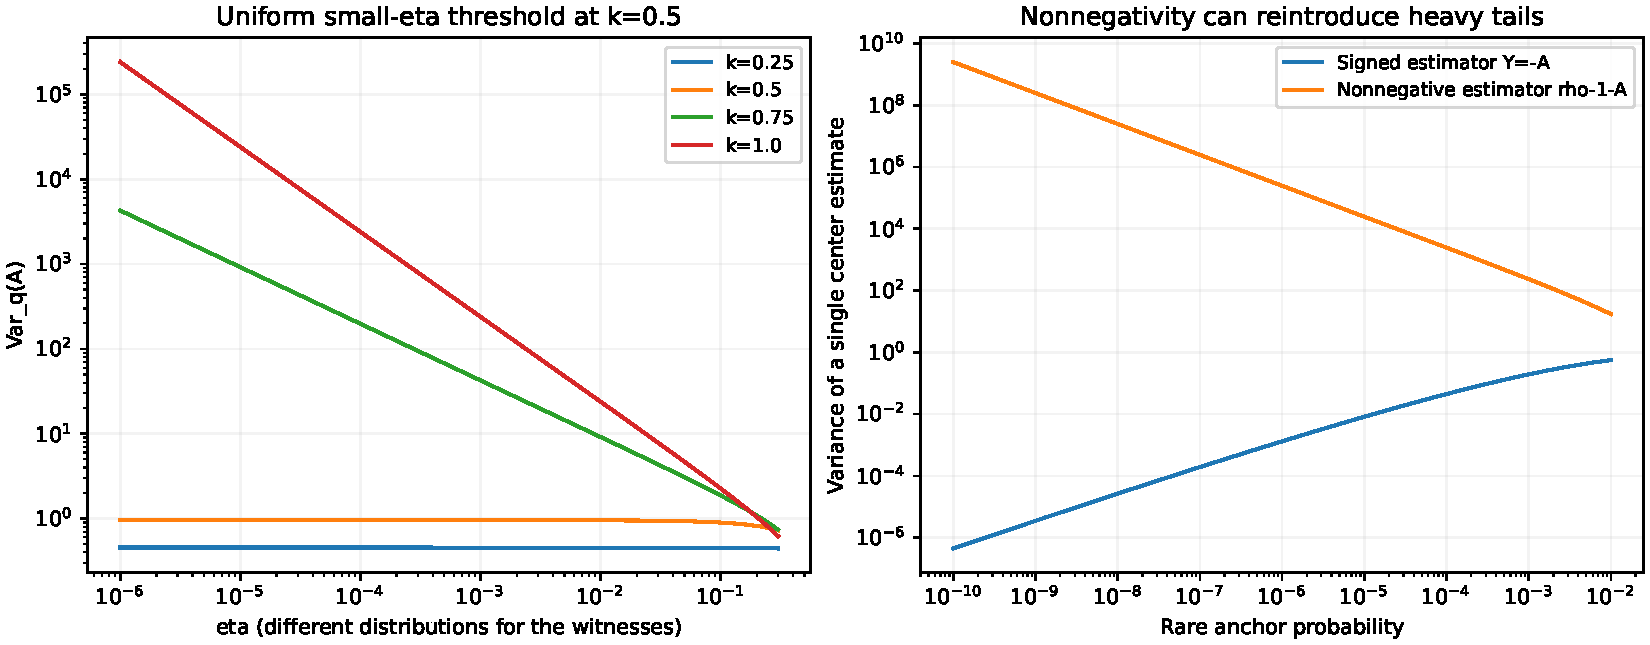
\includegraphics[width=\textwidth]{../../results/power-center-advantage/small-step-and-estimation.pdf}
 \caption{左：小步方差阈值的下界见证。右：在锚点提案 $q$ 下直接使用逐样本非负中心估计 $\widehat K_+$ 会重新引入概率比重尾，验证了混合包络提案 $\mu_c$ 的必要性。}
\end{figure}
\begin{figure}[htbp]
 \centering
 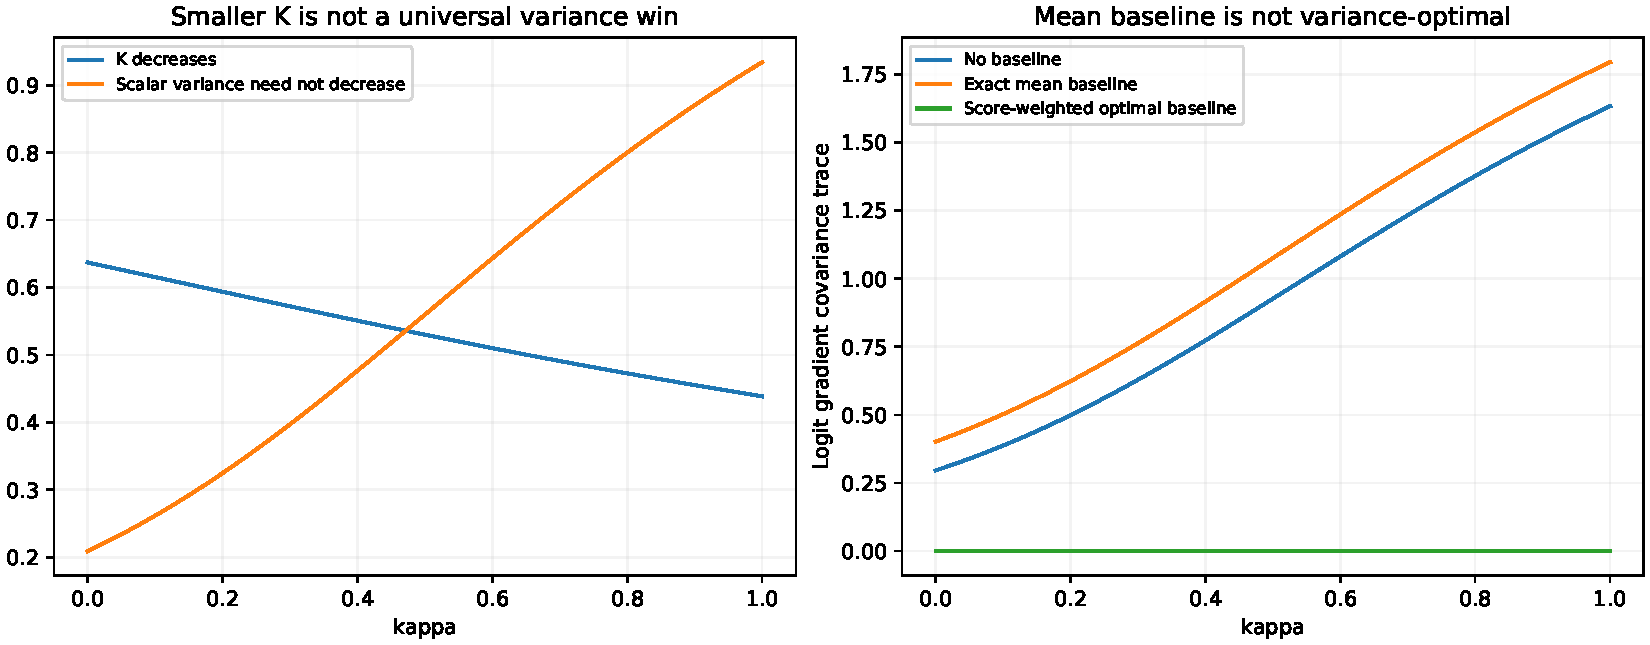
\includegraphics[width=\textwidth]{../../results/power-center-advantage/baseline-counterexample.pdf}
 \caption{同一二元输入下，$K_{\kappa,\eta}$ 随形状下降但标量方差不必下降；均值基线也不一定低于最优得分加权基线 $b_\star$ 的梯度方差。}
\end{figure}
\begin{figure}[htbp]
 \centering
 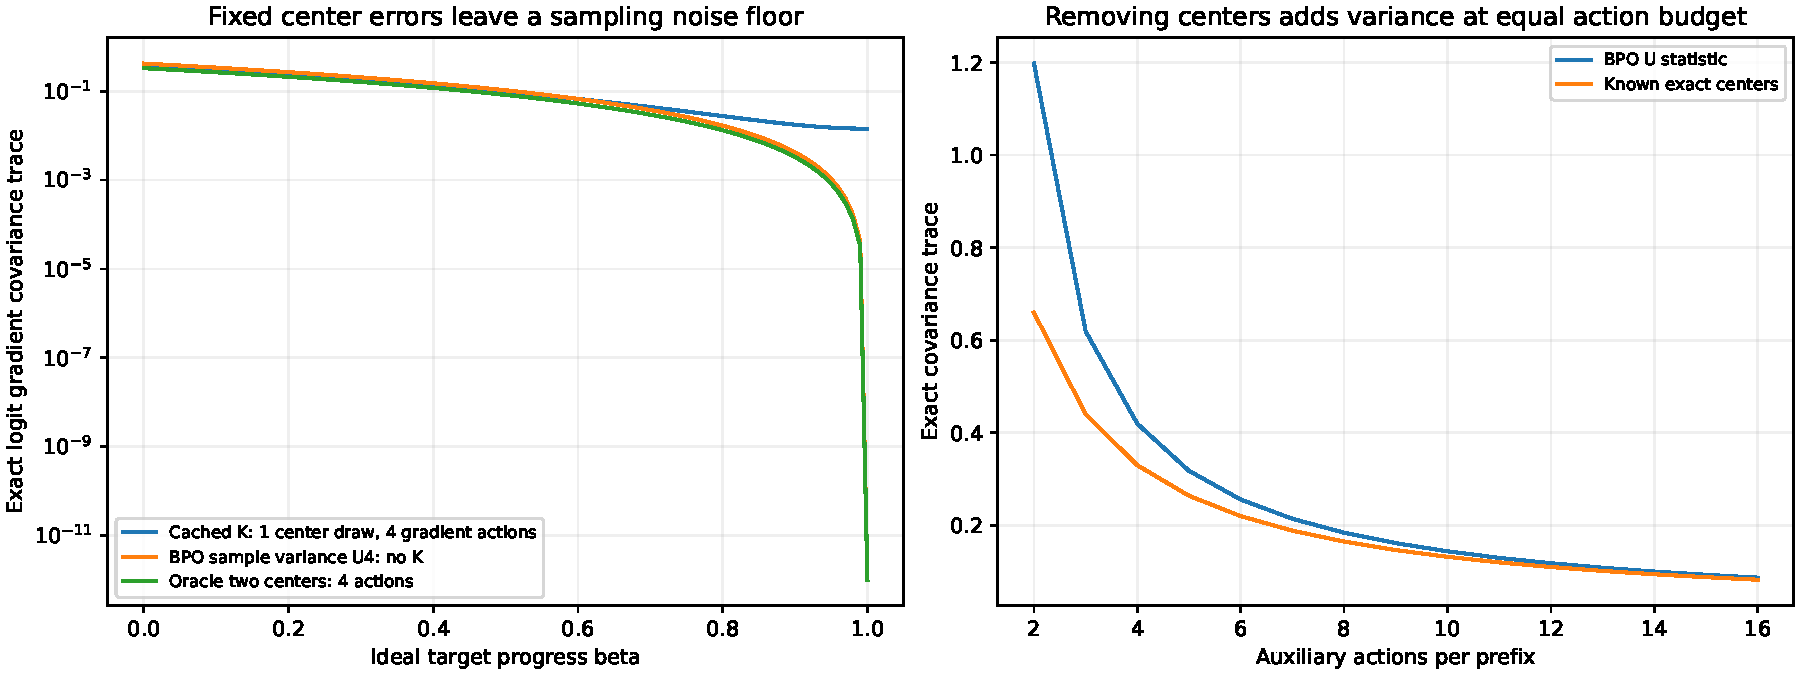
\includegraphics[width=\textwidth]{../../results/power-center-extensions/center-noise-and-sample-variance.pdf}
 \caption{左：理想 Logits 拟合路径上，固定教师中心估计误差产生末期采样噪声底，而 BPO 样本方差梯度的方差随残差平方同步归零。右：相同辅助动作数 $M$ 下取消两中心计算的 $O(M^{-2})$ 方差代价。}
\end{figure}

\chapter{OPD 算法谱系、稀疏缓存架构与生产实现契约}
\label{opd:chapter}

本章将前六章建立的内层投影理论、外层同步动力学与条件随机积分估计器落实为在线策略蒸馏（OPD）的完整算法谱系与生产级系统实现。首先在统一的外层--内层流水线（pipeline）下汇总七种 OPD 算法的采样测度、策略梯度系数与不动点，澄清 $\eta=1$ 与 $\eta\to\infty$ 两个端点处的精确行为；随后推导稀疏查询下配分函数对数 $\log Z_k$ 的 Delta-method 偏差、Cumulant（累积量）展开与尾部级数 U-统计量估计；接着证明生产级实现中用粗粒化 Tail-Aware 中心替换精确条件 KL 中心后所产生的梯度偏差与反对称 Jacobian（非保守更新场）；最后给出外层--内层主算法伪代码及分布式训练框架中的缓存与张量契约。

\section{OPD 七种算法的统一谱系与端点比较}
\label{opd:mirror-origin}
\label{sec:ch2-opd-specialization}
\label{sec:ch2-opd-baselines}

在第 $k$ 轮外层迭代中，系统冻结锚点 $q_k$ 并采样轨迹，对前缀 $s_t=(x,y_{<t})$ 与实际采样动作 $a_t=y_t$，冻结局部教师奖励为
\begin{equation}
\label{eq:ch2-opd-raw-reward}
r_k(s_t,a_t)=\log t(a_t\mid s_t)-\log q_k(a_t\mid s_t),
\qquad
\sum_{t=1}^H r_k(s_t,a_t)=\log t(y\mid x)-\log q_k(y\mid x).
\end{equation}
而随内层当前学生 $p_{k,n}$ 动态变化的即时奖励则记为 $r_{k,n}^{\mathrm{cur}}(s,a)=\log t(a\mid s)-\log p_{k,n}(a\mid s)=r_k(s,a)-U_{k,n}(s,a)$。注意对奖励做加性前缀基线平移
\begin{equation}
\label{eq:ch2-opd-centered-reward}
f_k^{\mathrm{ctr}}(s,a)=r_k(s,a)-b_k(s)
\end{equation}
仅将配分函数乘以 $e^{-\eta b_k(s)}$，不改变 Gibbs 目标分布；但若除以前缀标准差 $\sigma_k(s)>0$（即 $f_k^{\mathrm{std}}=(r_k-b_k)/\sigma_k$），则会将有效镜像步长改变为 $\eta/\sigma_k(s)$。因此 OPD 的标准实现仅做加性中心化。

我们将无镜像正则的两种当前奖励 OPD 基线（Token-IS OPD 与 On-Policy OPD）、删除镜像项后的冻结奖励基线（Frozen-Reward OPD, $\eta=+\infty$）以及四种有限 $\eta$ 镜像内层方法（PMD-Part、PMD-Mean、BPO、MDPO）统一归纳于表~\ref{tab:ch2-opd-seven-algorithms}。

\begin{table}[ht]
\centering
\caption{OPD 七种算法的训练测度、单样本策略梯度（PG）系数与精确内层不动点统一地图}
\label{tab:ch2-opd-baseline-map}
\label{tab:ch2-opd-seven-algorithms}
\begin{tabular}{>{\raggedright\arraybackslash}p{0.18\linewidth}>{\raggedright\arraybackslash}p{0.23\linewidth}>{\raggedright\arraybackslash}p{0.31\linewidth}>{\raggedright\arraybackslash}p{0.18\linewidth}}
\toprule
算法名称 & Rollout / 内层采样测度 & 单样本 PG 系数（乘在 $\nabla_\theta\log p_{k,n}$ 上） & 精确内层不动点 \\
\midrule
Token-IS OPD & 行为测度 $\beta_k$（或 $q_k$），$w=p_{k,n}/\beta_k$ & $-w\bigl(r_{k,n}^{\mathrm{cur}}+K_{pt,k,n}\bigr)$ & 最小化当前 $\KL(p\Vert t)$ \\
On-Policy OPD & 当前学生 $\beta_k=p_{k,n}$，$w=1$ & $-\bigl(r_{k,n}^{\mathrm{cur}}+K_{pt,k,n}\bigr)$ & Token-IS 在 $N=1$ 的特例 \\
Frozen-Reward ($\eta=+\infty$) & 锚点 $q_k$，$\omega_{k,n}=p_{k,n}/q_k$ & $-\omega_{k,n} r_k$ & 支集在 $\argmax_a r_k$ 上 \\
PMD-Part & 锚点 $q_k$ & $R^{\mathrm{Part}}=U_{k,n}-\eta r_k+\log Z_k$ & Gibbs 分布 $p_k^{\mathrm G}$ \\
PMD-Mean & 锚点 $q_k$ & $R^{\mathrm{Mean}}=U_{k,n}-\eta(r_k+K_{qt,k})$ & Lambert-$W$ 投影 $p_k^{\mathrm M}$ \\
BPO & 锚点 $q_k$ & $R^{\mathrm{BPO}}/\eta=(U_{k,n}+K_{qp,k,n})/\eta-(r_k+K_{qt,k})$ & Gibbs 分布 $p_k^{\mathrm G}$ \\
MDPO & 锚点 $q_k$，$\omega_{k,n}=p_{k,n}/q_k$ & $\omega_{k,n}(U_{k,n}/\eta-r_k)$ & Gibbs 分布 $p_k^{\mathrm G}$ \\
\bottomrule
\end{tabular}
\end{table}

\subsection{完整词表 Logits 路径与四个镜像内层的 PG 展开}
\label{sec:ch2-opd-full-vocab}
\label{subsec:ch2-opd-four-inner-pg}

当完整词表 Logits 可用时，配分函数对数为
\begin{equation}
\log Z_k(s)=\operatorname{logsumexp}_{v\in\mathcal V}
\bigl((1-\eta)\log q_k(v\mid s)+\eta\log t(v\mid s)\bigr),
\label{eq:ch2-opd-full-logz}
\end{equation}
对应的精确 Gibbs 不动点为
\begin{equation}
\label{eq:ch2-opd-common-mirror-solution}
p^{\star}_{k}(a\mid s)
=\frac{q_k(a\mid s)\exp(\eta r_k(s,a))}
{\mathbb E_{v\sim q_k}\exp(\eta r_k(s,v))}
\propto q_k(a\mid s)^{1-\eta}t(a\mid s)^{\eta}.
\end{equation}
三种回归残差与四种损失分别为：
\begin{align}
R_{k,n}^{\mathrm{Part}}(s,v)&=U_{k,n}(s,v)-\eta r_k(s,v)+\log Z_k(s),
\label{eq:ch2-opd-full-part-simplified}\\
R_{k,n}^{\mathrm{Mean}}(s,v)&=U_{k,n}(s,v)-\eta\bigl(r_k(s,v)+K_{qt,k}(s)\bigr),
\label{eq:ch2-opd-full-mean-simplified}\\
R_{k,n}^{\mathrm{BPO}}(s,v)&=U_{k,n}(s,v)+K_{qp,k,n}(s)-\eta\bigl(r_k(s,v)+K_{qt,k}(s)\bigr),
\label{eq:ch2-opd-full-bpo-residual,eq:ch2-opd-full-bpo-simplified,eq:ch2-opd-full-mdpo-simplified}
\end{align}
其中学生中心满足 $\nabla_\theta K_{qp,k,n}(s)=-\bar\psi_{k,n}(s)$（式~\eqref{eq:ch2-opd-grad-ktheta}）。四种镜像内层方法的完整策略梯度形式为：
\begin{align}
\nabla_\theta\mathcal L_{\mathrm{PMD\text{-}Part}}
&=\mathbb E_{d_k,q_k}\!\left[\sg\!\left(
U_{k,n}-\eta r_k+\log\mathbb E_{v\sim q_k}e^{\eta r_k(s,v)}
\right)\nabla_\theta\log p_{k,n}(a\mid s)\right],
\label{eq:ch2-opd-pg-pmd-part}\\
\nabla_\theta\mathcal L_{\mathrm{PMD\text{-}Mean}}
&=\mathbb E_{d_k,q_k}\!\left[\sg\!\left(
U_{k,n}-\eta[r_k+K_{qt,k}]\right)\nabla_\theta\log p_{k,n}(a\mid s)\right],
\label{eq:ch2-opd-pg-pmd-mean}\\
\nabla_\theta\mathcal L_{\mathrm{BPO}}
&=\mathbb E_{d_k,q_k}\!\left[\sg\!\left(
\frac{U_{k,n}+K_{qp,k,n}}\eta-r_k-K_{qt,k}\right)\nabla_\theta\log p_{k,n}(a\mid s)\right],
\label{eq:ch2-opd-full-bpo-gradient-simplified,eq:ch2-opd-bpo-descent-expanded,eq:ch2-opd-grad-ktheta,eq:ch2-opd-pg-bpo}\\
\nabla_\theta\mathcal L_{\mathrm{MDPO}}
&=\mathbb E_{d_k,q_k}\!\left[\sg\!\left(
\omega_{k,n}\left[\frac{U_{k,n}}\eta-r_k\right]\right)
\nabla_\theta\log p_{k,n}(a\mid s)\right],\qquad
\omega_{k,n}\coloneqq\frac{p_{k,n}}{q_k}=e^{U_{k,n}}.
\label{eq:ch2-opd-pg-mdpo,eq:ch2-omega-exp-u}
\end{align}

\subsection{OPD 基线算法：On-Policy OPD 与 Token-IS OPD}
\label{subsec:ch2-opd-baselines-in-map}
\label{subsec:ch2-opd-onpolicy-baseline}
\label{subsec:ch2-opd-is-baseline}

固定前缀 $s$ 上的无镜像逆向 KL 目标为
\begin{equation}
\label{eq:ch2-opd-baseline-objective}
J_s(\theta)=\operatorname{KL}(p_\theta\Vert t)
 =\mathbb E_{a\sim p_\theta}
 \left[\log p_\theta(a\mid s)-\log t(a\mid s)\right],
\end{equation}
其完整梯度为
\begin{equation}
\label{eq:ch2-opd-baseline-gradient}
\nabla_\theta J_s(\theta)
 =-\mathbb E_{a\sim p_\theta}
 \left[r_\theta^{\mathrm{cur}}(s,a)\nabla_\theta\log p_\theta(a\mid s)\right].
\end{equation}
引入动作无关的当前学生--教师逆向 KL 作为控制变量：
\begin{equation}
\label{eq:ch2-opd-vopd-center}
 K_{pt,k,n}(s)=\operatorname{KL}(p_\theta\Vert t).
\end{equation}
当采样来自行为策略 $\beta_k$（记 $w_{k,n}=p_{k,n}/\beta_k$）时，利用固定前缀下的重要性测度变换：
\begin{equation}
\label{eq:ch2-opd-token-is}
\mathbb E_{a\sim p_\theta}[h(a)]
 =\mathbb E_{a\sim \beta_k}
 \left[\frac{p_\theta(a\mid s)}{\beta_k(a\mid s)}h(a)\right],
\end{equation}
得到 Token-IS OPD 与 On-Policy OPD（$\beta_k=p_{k,n},\; w_{k,n}=1,\; N_{\mathrm{inner}}=1$）的策略梯度：
\begin{align}
\nabla_\theta\mathcal L_{\mathrm{Token\text{-}IS\text{-}OPD}}
&=-\mathbb E_{s\sim d_k,\,a\sim\beta_k}
\left[\sg\!\left(w_{k,n}(s,a)\bigl[r_{k,n}^{\mathrm{cur}}(s,a)+K_{pt,k,n}(s)\bigr]\right)
\nabla_\theta\log p_{k,n}(a\mid s)\right],
\label{eq:ch2-opd-is-pg,eq:ch2-token-is-opd-pg}\\
\nabla_\theta\mathcal L_{\mathrm{On\text{-}Policy\text{-}OPD}}
&=-\mathbb E_{s\sim d_k,\,a\sim p_{k,n}}
\left[\sg\!\left(r_{k,n}^{\mathrm{cur}}(s,a)+K_{pt,k,n}(s)\right)
\nabla_\theta\log p_{k,n}(a\mid s)\right].
\label{eq:ch2-onpolicy-opd-pg}
\end{align}

\begin{algorithm}[ht]
\caption{On-Policy OPD 基线\\{\small\textit{数学语义：每个外层步用当前学生重新采样 Rollout（$N_{\mathrm{inner}}=1$），无镜像近端正则}}}
\begin{algorithmic}[1]
\Require 提示分布 $\mathcal D$，教师 $t$，初始策略 $q_0$，外层步数 $K_{\mathrm{out}}$，批大小 $B_{\mathrm{batch}}$，最大长度 $H$
\Ensure 最终策略 $q_{K_{\mathrm{out}}}$
\For{$k=0,\ldots,K_{\mathrm{out}}-1$}
    \State 令 $q_k\gets p_{\theta_k}$ 并采样生成 $(s_i,a_i)$，其中 $a_i\sim q_k(\cdot\mid s_i)$
    \State 评估 $\log q_k(a_i\mid s_i)$、$\log t(a_i\mid s_i)$ 以及冻结支持估计 $\widehat K_{pt,k,0}(s_i)$
    \State $r_i\gets\log t(a_i\mid s_i)-\log q_k(a_i\mid s_i)$
    \State $g_k\gets-|\mathcal B_k|^{-1}\sum_i\sg\bigl(r_i+\widehat K_{pt,k,0}(s_i)\bigr)\nabla_{\theta_k}\log p_{\theta_k}(a_i\mid s_i)$
    \State $\theta_{k+1}\gets\operatorname{OptimizerStep}(\theta_k,g_k)$
\EndFor
\State \Return $q_{K_{\mathrm{out}}}$
\end{algorithmic}
\end{algorithm}

\begin{algorithm}[ht]
\caption{Token-IS OPD 基线\\{\small\textit{数学语义：复用锚点 Rollout 多步更新，仅通过 $p/q$ 修正固定前缀下的单步动作测度}}}
\begin{algorithmic}[1]
\Require 冻结锚点 $q=q_k$，教师 $t$，采样批次 $\mathcal B_k$，内层步数 $N_{\mathrm{inner}}$，学习率 $\{\alpha_{k,n}\}$
\Ensure 更新后参数 $\theta_{k+1}$
\State 初始化 $\theta\gets\theta_k$
\For{$n=0,\ldots,N_{\mathrm{inner}}-1$}
    \State 评估所有 $(s_i,a_i)\in\mathcal B_k$ 的 $\log p_\theta(a_i\mid s_i)$ 与冻结支持估计 $\widehat K_{pt,k,n}(s_i)$
    \State $u_i\gets\log p_\theta(a_i\mid s_i)-\log q(a_i\mid s_i)$,\quad $r_i\gets\log t(a_i\mid s_i)-\log p_\theta(a_i\mid s_i)$
    \State $w_i\gets\sg(\exp u_i)$
    \State $g_{k,n}\gets-|\mathcal B_k|^{-1}\sum_i\sg\bigl(w_i(r_i+\widehat K_{pt,k,n}(s_i))\bigr)\nabla_\theta\log p_\theta(a_i\mid s_i)$
    \State $\theta\gets\operatorname{OptimizerStep}(\theta,g_{k,n};\alpha_{k,n})$
\EndFor
\State \Return $\theta_{k+1}\gets\theta$
\end{algorithmic}
\end{algorithm}

\subsection{\texorpdfstring{$\eta=1$}{eta=1} 与 \texorpdfstring{$\eta\to+\infty$}{eta -> +infinity} 两个步长端点的精确对比}
\label{subsec:ch2-opd-eta-one-vopd}
\label{subsec:ch2-opd-eta-infinity}

\begin{proposition}[$\eta=1$ 时 MDPO 与 Token-IS OPD 的总体等价及 BPO/Mean 的多步分离]
\label{opd:objective-family}
\label{opd:eta-one-mdpo}
在同一固定前缀测度与锚点采样 $\beta_k=q_k$（即 $w_{k,n}=\omega_{k,n}=p_{k,n}/q_k$）下，当镜像步长取 $\eta=1$ 时：
\begin{enumerate}
\item \textbf{MDPO 与 Token-IS OPD 具有完全相同的总体梯度}：MDPO 系数为 $\omega_{k,n}(U_{k,n}-r_k)=-\omega_{k,n}r_{k,n}^{\mathrm{cur}}$，而 Token-IS vOPD 系数为
\begin{equation}
\label{eq:ch2-vopd-token-is-coef}
c_{\mathrm{vOPD}}(s,a)
=-\sg\!\left[
\omega_{k,n}(s,a)\bigl(r_{k,n}^{\mathrm{cur}}(s,a)+K_{pt,k,n}(s)\bigr)
\right].
\end{equation}
两者之差的锚点期望为 $\E_q[\frac{p}{q}K_{pt}\psi]=K_{pt}\sum_a p_a\nabla_\theta\log p_a=0$。
\item \textbf{BPO 与 PMD-Mean 在首步与 vOPD 重合、在后续内层步分离}：当 $\eta=1$ 时，BPO 与 PMD-Mean 的系数分别为
\begin{align}
c_{\mathrm{BPO}}(s,a)
&=U_{k,n}+K_{qp,k,n}-r_k-K_{qt,k}
 =-r_{k,n}^{\mathrm{cur}}+K_{qp,k,n}-K_{qt,k},
\label{eq:ch2-bpo-eta-one}\\
c_{\mathrm{PMD\text{-}Mean}}(s,a)
&=U_{k,n}-r_k-K_{qt,k}
 =-r_{k,n}^{\mathrm{cur}}-K_{qt,k}.
\label{eq:ch2-pmd-mean-eta-one}
\end{align}
在首步 $n=0$（$p_{k,0}=q_k$）处，$U_{k,0}=0,\;\omega_{k,0}=1,\;K_{qp,k,0}=0,\;K_{pt,k,0}=K_{qt,k}$，所有方法的逐动作系数均退化为 $-(r_k+K_{qt,k})$。但在 $n\ge 1$（$p_{k,n}\ne q_k$）时，它们的系数差为：
\begin{align}
c_{\mathrm{PMD\text{-}Mean}}-c_{\mathrm{vOPD}}
&=(\omega_{k,n}-1)r_{k,n}^{\mathrm{cur}}
 +\omega_{k,n}K_{pt,k,n}-K_{qt,k},\\
c_{\mathrm{BPO}}-c_{\mathrm{vOPD}}
&=(\omega_{k,n}-1)r_{k,n}^{\mathrm{cur}}
 +\omega_{k,n}K_{pt,k,n}-K_{qt,k}
 +K_{qp,k,n}.
\end{align}
\end{enumerate}
\end{proposition}

当 $\eta\to+\infty$ 时，镜像目标
\begin{equation}
\label{eq:ch2-opd-mirror-objective-eta}
F_{k,\eta}(p)=\frac{1}{\eta}\operatorname{KL}(p\Vert q)-\mathbb E_{a\sim p}[r_k(s,a)]
\end{equation}
删除了近端 KL 项，退化为冻结奖励线性目标与梯度：
\begin{align}
\label{eq:ch2-opd-frozen-reward-objective}
F_{k,\infty}(p)&=-\mathbb E_{a\sim p}[r_k(s,a)],\\
\label{eq:ch2-opd-frozen-reward-gradient}
\nabla_\theta F_{k,\infty}(p_\theta)
&=-\mathbb E_{s\sim d_k,\,a\sim q}
\left[\sg\!\left(\omega_\theta(s,a)r_k(s,a)\right)
\nabla_\theta\log p_\theta(a\mid s)\right].
\end{align}
记最大冻结奖励为 $m_k(s)=\max_{a:q(a)>0}r_k(s,a)$，最大动作集合为 $A_k(s)=\{a:r_k(s,a)=m_k(s)\}$。则 PMD-Part、BPO 与 MDPO 的有限 $\eta$ 精确 Gibbs 解在 $\eta\to+\infty$ 时收敛于最大奖励支集上的条件分布：
\begin{equation}
\lim_{\eta\to+\infty}p^\star_{\eta}(a\mid s)
=\frac{q(a\mid s)\,\mathbf 1\{r_k(s,a)=m_k(s)\}}
{q(A_k(s)\mid s)}.
\label{eq:ch2-opd-bpo-infinity-target}
\end{equation}
若固定当前参数 $p_\theta$ 直接取 BPO 下降方向的局部极限，则有：
\begin{equation}
-\nabla_\theta\mathcal L_{\mathrm{BPO}}
\longrightarrow
\mathbb E_{s\sim d_k,\,a\sim q}
\bigl[(r_k(s,a)+K_{qt,k}(s))\nabla_\theta\log p_\theta(a\mid s)\bigr].
\label{eq:ch2-opd-bpo-infinity-gradient}
\end{equation}而 PMD-Mean 的 $\eta\to+\infty$ 精确不动点极限则如第~\ref{ch:four-methods} 章命题~\ref{dyn:prop:mean-opd-large-eta} 所证，收敛于正部加权分布 $q(a\mid s)[r_k(s,a)+K_{qt,k}(s)]_+/H_+(s)$，不发生单点 Argmax 坍缩。

\section{稀疏查询下的条件 KL 与配分函数 \texorpdfstring{$\log Z_k$}{log Zk} 估计}
\label{sec:ch2-opd-z-kl-estimation}

固定前缀 $s$，令 $\mu(v)=q_k(v\mid s)$，$h(v)$ 为待求期望的被积函数，定义完整期望 $Q=\E_\mu[h]$、固定头部 $S_J$ 上的精确和 $Q_J^{\mathrm{head}}=\sum_{v\in S_J}\mu(v)h(v)$ 以及尾部均值 $\tau_J=\E_\mu[\mathbf1\{v\notin S_J\}h(v)]$。用 $m$ 个独立辅助锚点动作 $a_1,\ldots,a_m\overset{\mathrm{iid}}\sim\mu$ 构造尾部校正估计量：
\begin{equation}
\widehat Q_{J,m}=Q_J^{\mathrm{head}}+
\frac1m\sum_{j=1}^{m}\mathbf 1\{a_j\notin S_J\}h(a_j).
\label{eq:ch2-opd-generic-tail,eq:ch2-opd-generic-topk,eq:ch2-opd-topk-anchor-kl}
\end{equation}

\begin{theorem}[Top-$J$ 截断与尾部校正的偏差--方差分解]
\label{thm:ch2-opd-topk-bias-variance}
在 $\mathbb E_\mu[h^2]<\infty$ 且 $S_J$ 与辅助样本独立时，纯头部估计 $\widehat Q_J^{\mathrm{tr}}=Q_J^{\mathrm{head}}$ 与尾部校正估计 $\widehat Q_{J,m}$ 分别满足：
\begin{align}
\operatorname{Bias}(\widehat Q_J^{\mathrm{tr}})&=-\tau_J,&
\operatorname{Var}(\widehat Q_J^{\mathrm{tr}})&=0,&
\operatorname{MSE}(\widehat Q_J^{\mathrm{tr}})&=\tau_J^2,\\
\operatorname{Bias}(\widehat Q_{J,m})&=0,&
\operatorname{Var}(\widehat Q_{J,m})&=\frac{V_J}{m},&
\operatorname{MSE}(\widehat Q_{J,m})&=\frac{V_J}{m},
\end{align}
其中尾部修正方差为
\begin{equation}
V_J=\mathbb E_\mu\left[\mathbf 1\{v\notin S_J\}h(v)^2\right]-\tau_J^2.
\label{eq:ch2-opd-tail-variance}
\end{equation}
如果 $S_J\subseteq S_{J+1}$，则尾部二阶矩 $A_J=\mathbb E_\mu[\mathbf 1\{v\notin S_J\}h(v)^2]$ 单调不增，且 $V_J\le A_J$。尾部均值 $\tau_J$ 在 $h\ge0$ 时单调不增；对符号不定的 $h$，恒有 Cauchy--Schwarz 上界：
\begin{equation}
|\tau_J|\le \sqrt{\mu(S_J^c)A_J}.
\label{eq:ch2-opd-tail-cauchy}
\end{equation}
将 $h(v)$ 替换为得分加权向量 $h(v)\psi_{k,n}(v)$，同样得到向量梯度估计器的偏差与协方差：
\begin{equation}
\operatorname{Bias}(\widehat H_J^{\mathrm{tr}})
 =-\mathbb E_\mu\bigl[\mathbf 1\{v\notin S_J\}h(v)\psi_{k,n}(v)\bigr],
\qquad
\operatorname{Cov}(\widehat H_{J,m})
 =\frac1m\operatorname{Cov}_\mu\bigl(\mathbf 1\{v\notin S_J\}h(v)\psi_{k,n}(v)\bigr).
\label{eq:ch2-opd-gradient-topk-mse}
\end{equation}
\end{theorem}
\begin{proof}
记 $X_j=\mathbf1\{a_j\notin S_J\}h(a_j)$，由独立同分布性质有 $\E[X_j]=\tau_J$、$\Var(X_j)=V_J$，故 $\E[\widehat Q_{J,m}]=Q_J^{\mathrm{head}}+\tau_J=Q$ 且 $\Var(\widehat Q_{J,m})=V_J/m$。集合嵌套 $S_J\subseteq S_{J+1}$ 给出 $\mathbf1\{v\notin S_{J+1}\}\le\mathbf1\{v\notin S_J\}$，乘以非负 $h(v)^2$ 求期望即得 $A_{J+1}\le A_J$。对 $\mathbf1\{v\notin S_J\}$ 与 $\mathbf1\{v\notin S_J\}h(v)$ 应用 Cauchy--Schwarz 不等式即得式~\eqref{eq:ch2-opd-tail-cauchy}。
\end{proof}

对于配分函数
\begin{equation}
Z_k(s)=\mathbb E_{a\sim q_k(\cdot\mid s)}
\left[\left(\frac{t(a\mid s)}{q_k(a\mid s)}\right)^\eta\right],
\label{eq:ch2-opd-z-importance}
\end{equation}
令头部支持集为 $S_Z(s)$，构造无偏配分函数估计：
\begin{equation}
\widehat Z_{J,m}(s)
=\sum_{v\in S_Z(s)}q_k(v\mid s)^{1-\eta}t(v\mid s)^\eta
+\frac1m\sum_{j=1}^{m}\mathbf 1\{a_j\notin S_Z(s)\}
\left(\frac{t(a_j\mid s)}{q_k(a_j\mid s)}\right)^\eta,
\qquad a_j\sim q_k(\cdot\mid s).
\label{eq:ch2-opd-topk-z}
\end{equation}

\begin{theorem}[配分函数对数的 Plug-in 渐近偏差与方差]
\label{thm:ch2-opd-logz-delta}
设 $\widehat Z_{J,m}$ 为式~\eqref{eq:ch2-opd-topk-z} 的尾部校正无偏估计（$\mathbb E[\widehat Z_{J,m}]=Z_k>0$），在有限词表正支持与固定非空头部下，$\widehat Z_{J,m}$ 具有与 $m$ 无关的正下界与有限上界。记 $V_{J}=\operatorname{Var}_{q_k}(\mathbf 1\{a\notin S_Z\} (t(a\mid s)/q_k(a\mid s))^\eta)$。当 $m\to\infty$ 时：
\begin{align}
\mathbb E\bigl[\log\widehat Z_{J,m}\bigr]-\log Z_k
&=-\frac{V_J}{2mZ_k^2}+O(m^{-3/2}),\\
\operatorname{Var}\bigl(\log\widehat Z_{J,m}\bigr)
&=\frac{V_J}{mZ_k^2}+O(m^{-3/2}).
\end{align}
若改用纯头部截断估计 $Z_J^{\mathrm{tr}}=\sum_{v\in S_Z} q_k(v)^{1-\eta}t(v)^\eta$，则确定性偏差恒非正：$\log Z_J^{\mathrm{tr}}-\log Z_k\le 0$。
\end{theorem}
\begin{proof}
令零均值误差为 $\varepsilon_Z=\widehat Z_{J,m}-Z_k$，则 $\E[\varepsilon_Z]=0$、$\E[\varepsilon_Z^2]=V_J/m$ 且三阶绝对矩 $\E|\varepsilon_Z|^3=O(m^{-3/2})$。在 $Z_k>0$ 处作三阶泰勒展开 $\log(Z_k+\varepsilon_Z)=\log Z_k+\frac{\varepsilon_Z}{Z_k}-\frac{\varepsilon_Z^2}{2Z_k^2}+R_3$，取期望与方差即得两式。
\end{proof}

为消除 Plug-in 对数估计的 $O(m^{-1})$ Jensen 偏差，可利用累积量生成函数（cumulant-generating function）级数 $\log Z_k(s)=\sum_{j=1}^\infty\frac{\eta^j}{j!}\kappa_j(r_k)$（前两项为 $-\eta K_{qt,k}(s)+\frac{\eta^2}{2}\Var_{q_k}[r_k(s,a)]$），用 $m\ge L$ 个独立动作构造各阶无偏 $k$-统计量 $\widehat\kappa_j(r_k)$：
\begin{equation}
\widehat L_{L,m}(s)=\sum_{j=1}^{L}\frac{\eta^j}{j!}\widehat\kappa_j(r_k),
\qquad
\widehat L_{2,m}(s)=\eta\bar r_k(s)+\frac{\eta^2}{2}\,\widehat{\operatorname{Var}}\bigl(r_k(s,\cdot)\bigr).
\label{eq:ch2-opd-z-cumulant-start,eq:ch2-opd-logz-cumulant-series,eq:ch2-opd-logz-second-order,eq:ch2-opd-logz-kl-expansion,eq:ch2-opd-logz-kstat-estimator,eq:ch2-opd-logz-second-estimator}
\end{equation}

\begin{theorem}[Cumulant 截断估计器的偏差上界与方差]
\label{thm:ch2-opd-logz-cumulant}
固定有限词表且 $q_k(v\mid s),t(v\mid s)>0$。令 $\varphi(u)=\log\mathbb E_{q_k}[e^{u r_k}\mid s]$，指数倾斜分布为 $p_u(v\mid s)\propto q_k(v\mid s)e^{u r_k(s,v)}$。取固定阶数 $L\ge1$ 与样本数 $m\ge L$，则
\begin{align}
\mathbb E[\widehat L_{L,m}]-\log Z_k
&=-\frac{\eta^{L+1}}{L!}\int_0^1(1-u)^L\varphi^{(L+1)}(u\eta)\,du,\\
\bigl|\mathbb E[\widehat L_{L,m}]-\log Z_k\bigr|
&\le\frac{|\eta|^{L+1}}{(L+1)!}\sup_{u\in[0,\eta]}\bigl|\kappa_{L+1}^{p_u}(r_k)\bigr|,\qquad
\operatorname{Var}(\widehat L_{L,m})=O(m^{-1}).
\end{align}
进一步，定义非空头部质量与尾部均值
\begin{equation*}
Z_H=\sum_{v\in S_Z}q_k(v)^{1-\eta}t(v)^\eta>0,\qquad
\tau=\E_{q_k}[u(a)],\qquad
u(a)=\mathbf1\{a\notin S_Z\}(t(a)/q_k(a))^\eta.
\end{equation*}
当 $\kappa_Z=\tau/Z_H<1$ 时，使用无偏对称 U-统计量
\begin{equation*}
\widehat{\tau^\ell}=\binom{m}{\ell}^{-1}\sum_{1\le i_1<\cdots<i_\ell\le m}\prod_{q=1}^\ell u(a_{i_q})
\end{equation*}
构造尾部幂级数估计器：
\begin{equation}
\widehat L_{J,L}(s)=\log Z_H+
\sum_{\ell=1}^{L}\frac{(-1)^{\ell+1}}{\ell Z_H^\ell}
\widehat{\tau^\ell},\qquad
\bigl|\mathbb E[\widehat L_{J,L}]-\log Z_k\bigr|
\leq \frac{\kappa_Z^{L+1}}{(L+1)(1-\kappa_Z)}.
\label{eq:ch2-opd-logz-tail-series,eq:ch2-opd-logz-tail-series-estimator,eq:ch2-opd-logz-tail-remainder}
\end{equation}
\end{theorem}
\begin{proof}
对指数倾斜族求导可得 $\varphi^{(j)}(u)=\kappa_j^{p_u}(r_k)$。由带积分余项的 $L$ 阶泰勒公式及无偏 $k$-统计量的性质 $\E[\widehat\kappa_j(r_k)]=\varphi^{(j)}(0)$，立得偏差积分公式与绝对值上界。同理，对 $\log Z_k=\log Z_H+\log(1+\tau/Z_H)$ 展开墨卡托级数并代入 $\E[\widehat{\tau^\ell}]=\tau^\ell$，余项由几何级数控制即得式~\eqref{eq:ch2-opd-logz-tail-remainder}。
\end{proof}

\section{Tail-Aware 中心的梯度偏差、非保守更新场与主算法}
\label{opd:approximate-field}

固定前缀 $s$ 与内层步，简写 $q=q_k(\cdot\mid s),\; p=p_{k,n}(\cdot\mid s),\; t=t(\cdot\mid s)$。设头部支持集 $S_J$ 由冻结锚点 $q$ 选出，定义两个被 Tail-Aware 中心遗漏的非负尾部条件形状 KL：
\begin{align}
 b_J^T(s)=\epsilon_T(s)&=q(S_J^c)\KL\bigl(q(\cdot\mid S_J^c)\Vert t(\cdot\mid S_J^c)\bigr)=K_{qt,k}-\widehat K_{qt,k}\ge 0,\\
 b_{J,n}^S(s)=\epsilon_S(s)&=q(S_J^c)\KL\bigl(q(\cdot\mid S_J^c)\Vert p(\cdot\mid S_J^c)\bigr)=K_{qp,k,n}-\widehat K_{qp,k,n}\ge 0.
\end{align}

\begin{theorem}[Tail-Aware Mean/BPO 解析更新的梯度偏差]
\label{thm:ch2-ta-center-gradient-bias}
令 $g_{\mathrm{Mean}}(s)$、$g_{\mathrm{BPO}}(s)$ 为使用精确条件 KL 中心的得分函数梯度，$\widehat g_{\mathrm{Mean}}(s)$、$\widehat g_{\mathrm{BPO}}(s)$ 为替换成 Tail-Aware 中心并对整个权重停止梯度后的条件期望。则：
\begin{align}
 \widehat g_{\mathrm{Mean}}(s)-g_{\mathrm{Mean}}(s)
 &=\eta b_J^T(s)\mathbb E_{a\sim q}\bigl[\nabla_\theta\log p(a)\bigr],\\
 \widehat g_{\mathrm{BPO}}(s)-g_{\mathrm{BPO}}(s)
 &=\left(b_J^T(s)-\frac{b_{J,n}^S(s)}{\eta}\right)
   \mathbb E_{a\sim q}\bigl[\nabla_\theta\log p(a)\bigr].
\end{align}
相应的近似 BPO 残差 $\widehat R_{k,n}^{\mathrm{BPO}}(a)=\log\frac{p(a)}{q(a)}+\widehat K_{qp,k,n}-\eta\bigl(\log\frac{t(a)}{q(a)}+\widehat K_{qt,k}\bigr)$ 满足非零均值：
\begin{equation}
 \mathbb E_q\bigl[\widehat R_{k,n}^{\mathrm{BPO}}\bigr]=-b_{J,n}^S(s)+\eta b_J^T(s).
\end{equation}
\end{theorem}
\begin{proof}
代入 $\widehat K_{qt,k}=K_{qt,k}-b_J^T$ 与 $\widehat K_{qp,k,n}=K_{qp,k,n}-b_{J,n}^S$，逐动作有 $\widehat R_{k,n}^{\mathrm{Mean}}(a)=R_{k,n}^{\mathrm{Mean}}(a)+\eta b_J^T$ 以及 $\widehat R_{k,n}^{\mathrm{BPO}}(a)=R_{k,n}^{\mathrm{BPO}}(a)-b_{J,n}^S+\eta b_J^T$。因精确残差满足 $\E_q[R_{k,n}^{\mathrm{BPO}}]=0$，对近似残差取期望即得 $-b_{J,n}^S+\eta b_J^T$；分别乘以 $\nabla_\theta\log p(a)$（BPO 再除以 $\eta$）并在冻结分布 $q$ 下取期望即得两个梯度偏差公式。
\end{proof}

\begin{proposition}[Tail-Aware BPO 近似平方损失求导与停止梯度 PG 更新的区别]
\label{prop:ch2-ta-square-versus-sg}
\label{opd:approximate-square}
若对近似学生 Tail-Aware 中心 $\widehat K_{qp,k,n}$ 保留梯度，直接对近似平方目标 $\widehat{\mathcal L}_{\mathrm{BPO}}(s)=\frac1{2\eta}\mathbb E_q[(\widehat R_{k,n}^{\mathrm{BPO}})^2]$ 求完整参数梯度，则：
\begin{equation}
 \nabla_\theta\widehat{\mathcal L}_{\mathrm{BPO}}(s)
 =\widehat g_{\mathrm{BPO}}(s)
 +\frac{\mathbb E_q[\widehat R_{k,n}^{\mathrm{BPO}}]}{\eta}\nabla_\theta\widehat K_{qp,k,n}(s)
 =\widehat g_{\mathrm{BPO}}(s)
 +\left(b_J^T(s)-\frac{b_{J,n}^S(s)}{\eta}\right)
   \nabla_\theta\widehat K_{qp,k,n}(s).
\end{equation}
\end{proposition}
\begin{proof}
因 $q,t,S_J$ 均冻结，$\nabla_\theta\widehat R_{k,n}^{\mathrm{BPO}}(a)=\nabla_\theta\log p(a)+\nabla_\theta\widehat K_{qp,k,n}$。应用链式法则得 $\nabla_\theta\widehat{\mathcal L}_{\mathrm{BPO}}=\frac1\eta\E_q[\widehat R_{k,n}^{\mathrm{BPO}}\nabla_\theta\log p]+\frac1\eta\E_q[\widehat R_{k,n}^{\mathrm{BPO}}]\nabla_\theta\widehat K_{qp,k,n}$，代入定理~\ref{thm:ch2-ta-center-gradient-bias} 的残差均值即得结论。
\end{proof}

\begin{theorem}[粗粒化中心替换后的更新场反对称 Jacobian 与非保守性]
\label{opd:field-curl}
固定 $q,t$ 和头部 $S_J$，记精确学生中心为 $K=\KL(q\Vert p)$，尾部形状误差为 $\epsilon_S=b_{J,n}^S=K-\widehat K_S$、$\epsilon_T=b_J^T=K_{qt}-\widehat K_T$。则生产 BPO 的条件期望更新场可写为
\begin{equation}
\widehat g=\nabla_\theta \mathcal L_{\mathrm{BPO}}-\epsilon_T\nabla_\theta K+\frac{\epsilon_S}{\eta}\nabla_\theta K.
\end{equation}
以 Jacobian 约定 $(D\widehat g)_{ij}=\partial \widehat g_i/\partial\theta_j$，其反对称部分（旋度）恒为：
\begin{equation}
D\widehat g-(D\widehat g)^\top
=\eta^{-1}\Bigl[\nabla_\theta K(\nabla_\theta\epsilon_S)^\top-\nabla_\theta\epsilon_S(\nabla_\theta K)^\top\Bigr].
\end{equation}
当该矩阵非零时，参数空间邻域内不存在任何二次连续可微的固定标量势函数使其欧氏梯度等于 $\widehat g$。
\end{theorem}
\begin{proof}
由 $\nabla_\theta K=-\E_q[\psi]$ 及定理~\ref{thm:ch2-ta-center-gradient-bias} 立得 $\widehat g$ 的表达式。由于 $\epsilon_T$ 在内层冻结，前两项是标量函数 $\mathcal L_{\mathrm{BPO}}-\epsilon_T K$ 的梯度，其二阶偏导对称。对第三项乘积求导：$\partial_j(\epsilon_S\partial_i K)=(\partial_j\epsilon_S)(\partial_i K)+\epsilon_S\partial_j\partial_i K$，交换 $(i,j)$ 相减消去对称的 $\epsilon_S\partial_j\partial_i K$，即得反对称外积差公式。
\end{proof}

\begin{example}[三 Token 粗粒化 BPO 的非零旋度精确算例]
\label{opd:curl-example}
取三元词表 $q=(0.5,0.3,0.2),\; t=(0.2,0.3,0.5)$，头部 $S_1=\{0\}$，$\eta=0.7$，学生 Logits $z=(-0.3,0.6,0)$，以 $(z_0,z_1)$ 为自由坐标。记尾部质量 $Q=q_1+q_2=0.5,\; P=p_1+p_2$。粗粒化中心为 $\widehat K_S=q_0\log(q_0/p_0)+Q\log(Q/P)$，尾部形状误差为 $\epsilon_S=\sum_{a=1}^2 q_a\log(q_a/p_a)-Q\log(Q/P)$。改变 $z_0$ 仅缩放尾部总质量 $P$ 而尾内条件比例不变，故 $\partial_0\epsilon_S=0$；对 $z_1$ 微分尾内比例得 $\partial_1\epsilon_S=Q\frac{p_1}{P}-q_1$，且 $\partial_0 K=p_0-q_0$。因此旋度为：
\begin{equation}
\partial_1\widehat g_0-\partial_0\widehat g_1
=\frac{(p_0-q_0)(Q p_1/P-q_1)}{\eta}
=-0.0095250968566\ne 0.
\end{equation}
直接由 $\log\operatorname{softmax}$ 自动微分计算条件更新场的 Jacobian 矩阵为：
\begin{equation}
D\widehat g=
\begin{pmatrix}
0.3491477001&-0.2186486876\\
-0.2091235908&0.2947641411
\end{pmatrix},
\end{equation}
其交叉偏导之差与解析公式完全一致。
\end{example}

\begin{algorithm}[ht]
\caption{Tail-Aware OPD 外层--内层主优化算法\\{\small\textit{数学语义：冻结外层 Rollout，以 Tail-Aware KL 中心运行 Mean、BPO 或 MDPO，再同步并重新 Rollout}}}
\begin{algorithmic}[1]
\Require 提示分布 $\mathcal D$，教师 $t$，初始学生 $q_0=p_{\theta_{0,0}}$，外层步数 $K_{\mathrm{out}}$，批大小 $B_{\mathrm{batch}}\ge1$，最大长度 $H\ge1$，方法 $M\in\{\mathrm{Mean},\mathrm{BPO},\mathrm{MDPO}\}$，$\eta>0$，内层步数 $N_{\mathrm{inner}}\ge1$，学习率 $\{\alpha_{k,n}\}$，同步模式 $\mathrm{Sync}\in\{\mathrm{hard},\mathrm{soft}\}$（权重 $\zeta\in(0,1]$）
\Ensure 最终策略 $q_{K_{\mathrm{out}}}$ 与参数 $\theta_{K_{\mathrm{out}}}$
\For{$k=0,\ldots,K_{\mathrm{out}}-1$}
    \State $\mathcal B_k\gets\varnothing$
    \For{$i=1,\ldots,B_{\mathrm{batch}}$}
        \State 采样提示 $x_i\sim\mathcal D$，按 $a_{i,t}\sim q_k(\cdot\mid s_{i,t})$ 生成 $y_i=(a_{i,1},\ldots,a_{i,\tau_i})$（在 EOS 或长度 $H$ 终止）
        \State $\mathcal B_k\gets\mathcal B_k\mathbin{\uplus}\{(s_{i,t},a_{i,t}):1\le t\le\min(\tau_i,H)\}$
    \EndFor
    \State 若 $\mathcal B_k=\varnothing$ 则报错终止；否则定义经验分布 $\widehat d_k$ 赋予 $\mathcal B_k$ 中每个前缀出现位置相等权重
    \State $\theta_{k,0}\gets\theta_k$；查询并冻结 $S_J(s)=\operatorname{TopJ}(q_k(\cdot\mid s))$ 上的 $\log q_k(v\mid s),\log t(v\mid s)$、尾部质量及采样动作的 $\log t(a\mid s),\log q_k(a\mid s)$，释放完整词表 Logits
    \State 使用同一 $S_J(s)$ 和尾部总质量计算并冻结 $\widehat K_{qt,k}(s)\gets\mathcal K_J^{\mathrm{TA}}(q_k(\cdot\mid s)\Vert t(\cdot\mid s))$
    \For{$n=0,\ldots,N_{\mathrm{inner}}-1$}
        \State 在冻结 $S_J(s)$ 上计算当前 $\log p_{k,n}(v\mid s)$ 与 $\widehat K_{qp,k,n}(s)\gets\mathcal K_J^{\mathrm{TA}}(q_k\Vert p_{k,n})$
        \If{$M=\mathrm{Mean}$}
            \State $g_{k,n}\gets\frac1{|\mathcal B_k|}\sum_{(s,a)\in\mathcal B_k}\sg\!\left(\log\frac{p_{k,n}(a\mid s)}{q_k(a\mid s)}-\eta\left(\log\frac{t(a\mid s)}{q_k(a\mid s)}+\widehat K_{qt,k}(s)\right)\right)\nabla_{\theta_{k,n}}\log p_{k,n}(a\mid s)$
        \ElsIf{$M=\mathrm{BPO}$}
            \State $\begin{aligned}g_{k,n}\gets\frac1{|\mathcal B_k|}\sum_{(s,a)\in\mathcal B_k}&\sg\!\left(\eta^{-1}\left(\log\frac{p_{k,n}(a\mid s)}{q_k(a\mid s)}+\widehat K_{qp,k,n}(s)\right)-\log\frac{t(a\mid s)}{q_k(a\mid s)}-\widehat K_{qt,k}(s)\right)\\&{}\cdot\nabla_{\theta_{k,n}}\log p_{k,n}(a\mid s)\end{aligned}$
        \ElsIf{$M=\mathrm{MDPO}$}
            \State $\begin{aligned}g_{k,n}\gets\frac1{|\mathcal B_k|}\sum_{(s,a)\in\mathcal B_k}&\sg\!\left(\frac{p_{k,n}(a\mid s)}{q_k(a\mid s)}\left(\eta^{-1}\log\frac{p_{k,n}(a\mid s)}{q_k(a\mid s)}-\log\frac{t(a\mid s)}{q_k(a\mid s)}\right)\right)\\&{}\cdot\nabla_{\theta_{k,n}}\log p_{k,n}(a\mid s)\end{aligned}$
        \EndIf
        \State $\theta_{k,n+1}\gets\operatorname{OptimizerStep}(\theta_{k,n},g_{k,n};\alpha_{k,n})$
    \EndFor
    \If{$\mathrm{Sync}=\mathrm{hard}$}
        \State $\theta_{k+1}\gets\theta_{k,N_{\mathrm{inner}}}$ 且 $q_{k+1}\gets p_{\theta_{k+1}}$
    \Else
        \State 对每个前缀 $s$ 令 $q_{k+1}(\cdot\mid s)\gets(1-\zeta)q_k(\cdot\mid s)+\zeta p_{k,N_{\mathrm{inner}}}(\cdot\mid s)$
    \EndIf
\EndFor
\State \Return $(q_{K_{\mathrm{out}}},\theta_{K_{\mathrm{out}}})$
\end{algorithmic}
\end{algorithm}

\begin{algorithm}[ht]
\caption{OPD 纯采样动作（Sampled-Token）内层更新\\{\small\textit{数学语义：每个前缀仅访问 Rollout 的采样动作及同前缀辅助动作}}}
\begin{algorithmic}[1]
\Require 冻结锚点 $q_k$，教师 $t$，Rollout 样本对 $(s_i,a_i)$，方法 $M$，中心样本数 $m$，步长 $\eta$
\Ensure 更新后的学生参数 $\theta$
\For{每个前缀 $s_i$}
    \State 读取 $\log t(a_i\mid s_i)$ 与 $\log q_k(a_i\mid s_i)$，令 $r_i\gets\log t(a_i\mid s_i)-\log q_k(a_i\mid s_i)$
    \If{$M=\mathrm{Mean}$}
        \State 在同一前缀获取独立辅助动作估计冻结奖励中心 $\widehat{\bar r}_i$,$\ell_i\gets\frac12\bigl[U_{k,n}(s_i,a_i)-\eta\sg(r_i-\widehat{\bar r}_i)\bigr]^2$
    \ElsIf{$M=\mathrm{BPO}$}
        \State 在同一前缀估计奖励中心与可微学生中心，按 BPO 内层算法的有限样本修正因子构造带 $1/(2\eta)$ 的平方损失 $\ell_i$
    \ElsIf{$M=\mathrm{MDPO}$}
        \State $w_i\gets\sg\bigl(p_{k,n}(a_i\mid s_i)/q_k(a_i\mid s_i)\bigr)$，$\ell_i\gets\sg\bigl(w_i[\eta^{-1}\log(p_{k,n}(a_i\mid s_i)/q_k(a_i\mid s_i))-r_i]\bigr)\log p_{k,n}(a_i\mid s_i)$
    \ElsIf{$M=\mathrm{Part}$}
        \State 估计或加载前缀配分基线 $\widehat{\log Z_i}$，令 $\ell_i\gets\frac12\bigl[\eta r_i-\widehat{\log Z_i}-U_{k,n}(s_i,a_i)\bigr]^2$
    \EndIf
\EndFor
\State 在保持 $q_k$ 与 $t$ 冻结下对 $B^{-1}\sum_i\ell_i$ 执行梯度下降并返回 $\theta$
\end{algorithmic}
\end{algorithm}

\section{生产级缓存架构、序列位置对齐与分布式张量契约}
\label{opd:production-contract}

本项目的代码库将可枚举数学 Oracle 与大规模分布式训练算子严格分离：
\begin{enumerate}
\item \textbf{参考 Oracle 与生产算子白名单}：数学 Oracle 位于 \path{src/mirroropd/token_inner.py}（支持 Part、Mean、BPO、MDPO 四种总体损失）；生产算子位于 \path{src/mirroropd/training/losses.py}，支持 \path{pmd_mean}、\path{bpo}、\path{mdpo}、\path{opd_onpolicy}、\path{opd_is}、\path{opd_is_no_baseline} 六种模式（白名单不含需要额外估计 $\log Z_k$ 的 Part）。
\item \textbf{Anchor-to-Teacher 路由与 $O(BHJ)$ 缓存压缩}：\path{src/mirroropd/training/cache.py} 首先从锚点 $q_k$ 的完整 Logits 构造冻结 Top-$J$ 头部 IDs、头部对数概率、尾部对数总质量、采样动作对数概率与有效位置掩码（mask）。随后教师 Worker 在完全相同的 Tokenizer 与词表下对\textbf{锚点选出的头部 IDs} 及采样动作打分（不可用教师自身的 Top-$J$ 替代锚点请求的 IDs）。传输与缓存开销从全词表的 $O(BH|\mathcal V|)$（如 $|\mathcal V|=150{,}000$、FP16、8192 长度单序列约 $2.46$ GB）降至 $O(BHJ)$。
\item \textbf{采样温度、全支持要求与 verl FSDP 对齐}：所有 Logits 必须先除以同一正采样温度再计算 $\log\operatorname{softmax}$；完整支持语义要求 \path{do_sample=True, top_p=1, top_k=-1}。\path{src/mirroropd/integrations/verl/fsdp.py} 将缓存与 Logits 按预测位置（prediction position）严格对齐，在执行 \path{gather} 前排除所有 Prompt、Padding 与终止符后的无效位置，并在本地完整词表上归约（而非在未同步的 Tensor-Parallel 词表分片上独立计算）。
\item \textbf{单元测试覆盖}：\path{tests/test_upstream_opd_semantics.py}、\path{tests/test_upstream_mirror_wiring.py} 与 \path{tests/test_mdpo_eta_limits.py} 分别对全支持梯度端点、非保守场残差、无效位置零梯度、路由契约与 $\eta\in\{1,\infty\}$ 极限进行回归验证。
\end{enumerate}

\part{数值审计、语言模型实验与证据边界}

\chapter{精确可枚举系统的数值审计与动力学核验}
\label{evidence:chapter}

为了将数学定理、算法实现与大模型经验训练现象严格区分开来，第三篇按照证据强度由确定性精确核验向大规模神经网络系统递进。本章集中所有\textbf{可完整枚举词表、零采样噪声或受控随机注入的精确数值实验}（第 8 章），下一章则集中真实语言模型（Qwen3、Pythia、DeepSeek）上的估计器对照、标量调度验证与 ResOPD 端到端推理基准实验（第 9 章）。

\section{三层实验数据集体系与可证伪审计协议}
\label{evidence:toy}

本项目的实验图与表不能直接从一批混合的 Rollout 日志中生成，每一张图都必须明确标注其使用的策略、前缀访问测度以及词表信息访问模式。实验输入按由易到难严格划分为三层：
\begin{enumerate}
\item \textbf{第一层：可枚举 Categorical Oracle（零文本数据、零模型 Rollout）}。固定单个前缀 $s$，直接生成锚点、教师与学生的完整词表 Logits，并通过 Softmax 得到精确概率向量 $q_k(\cdot\mid s)$、$t(\cdot\mid s)$ 与 $p_{k,n}(\cdot\mid s)$。每个前缀保存完整概率向量、两个对数概率向量以及精确积分真值：
\begin{align}
K_{qt,k}(s)&=\operatorname{KL}(q_k\Vert t),\qquad K_{qp,k,n}(s)=\operatorname{KL}(q_k\Vert p_{k,n}),\\
\log Z_k(s)&=\log\sum_{v\in\mathcal V}\exp\bigl((1-\eta)\log q_k(v\mid s)+\eta\log t(v\mid s)\bigr).
\end{align}
该层提供所有估计量与代数恒等式的精确真值（Ground Truth），专门用于以机器精度（$10^{-15}$）核验偏差、方差、均方误差、梯度旋度与外层硬同步渐近阶数。
\item \textbf{第二层：冻结外层轮次的真实语言模型前缀数据}。先选定一个不参与训练的独立提示文件 $\mathcal X=\{x_i\}_{i=1}^{N_x}$，用当前锚点 $q_k$ 对每个提示采样生成回复轨迹，得到
\begin{equation}
s_{i,t}=(x_i,y_{i,<t}),\qquad a_{i,t}=y_{i,t},\qquad a_{i,t}\sim q_k(\cdot\mid s_{i,t}).
\end{equation}
保存 Prompt ID、Token IDs、注意力掩码、回复掩码、前缀长度、锚点与教师对采样 Token 的对数概率以及（在审计模式下）完整词表分布。同一前缀的多个后继 Token 样本才能用于估计条件期望；不同前缀只能在外层按照经验访问测度 $\widehat d_k$ 聚合。
\item \textbf{第三层：完整的 OPD 外层--内层闭环训练}。第 $k$ 轮仅使用 $q_k$ 生成 Rollout，缓存该轮前缀集合和锚点/教师的 Token 级对数概率摘要；随后固定这批数据运行 $N$ 个内层步得到 $p_{k,N}$，再执行硬同步或软同步得到 $q_{k+1}$ 并重新生成下一轮 Rollout，从而产出完整的动力学序列：
\begin{equation}
\bigl\{(\widehat d_k,q_k,p_{k,n},t):\; k=0,\ldots,K_{\mathrm{out}}-1,\ n=0,\ldots,N\bigr\}.
\end{equation}
\end{enumerate}

\subsection{正式语言模型实验前的七项数学与实现前置核验}

在运行任何语言模型训练之前，代码必须逐项通过以下七项自动化 Oracle 测试：
\begin{enumerate}
\item 对随机 Categorical Logits，核对 PMD-Mean 的 Lambert-$W$ 归一化、KKT 条件与最优点零梯度；核对 Mean/BPO 的损失及梯度差异恒等式（\path{tests/test_mean_bpo.py} 覆盖词表维数 $V\in\{2,4,8\}$、镜像系数 $\eta\in\{0.1,0.5,1,2\}$ 共 48 组随机问题，同时验证解析梯度、逐坐标有限差分、Part/BPO 的 Gibbs 零损失、初始化方向尺度、恒定信号、完整枚举的有限样本修正与 Off-Behavior 双样本重要性权重）；
\item 对随机 Categorical Logits，核对 PMD-Part 的 \path{logsumexp} 目标与显式求和一致；
\item 对随机正支持分布 $P,Q$，用大样本核对 K4 数值与精确 $\KL(P\Vert Q)$ 的误差按 $O(B^{-1/2})$ 衰减；
\item 用自动微分与有限差分核对 K4 梯度，而非仅检查标量前向值（\path{tests/test_kl_estimators.py} 使用 $200{,}000$ 个 Token 样本核验 K4，实测绝对数值误差为 $5.6\times 10^{-5}$，梯度 $\ell_2$ 误差为 $1.5\times 10^{-3}$）；
\item 检查固定锚点采样的重要性权重校正在 $p/q$ 偏离 $1$ 时的无偏性；
\item 人为改变学生与锚点的偏离程度，测量 $\chi^2(p\Vert q)$ 与重要性加权估计方差；
\item 硬同步后重新采样 Rollout，确认新一轮残差使用更新后的锚点 $q_{k+1}$ 而非上一轮缓存的对数概率。
\end{enumerate}

\section{四目标商坐标恒等式、局部曲率与非保守更新场的精确核验}
\label{evidence:reconstruction}

本节对应实验目录 \path{results/book-reconstruction/}（完整参数、随机种子、词表规模、误差定义与代码版本保存于 \path{results/book-reconstruction/metadata.json}）。实验在固定前缀的完整动作枚举下遍历 $360$ 组分布与参数配置，逐项核验：
\begin{itemize}
\item \textbf{商坐标分解与二阶曲率恒等式}：全面核对 Part--BPO 与 Mean--BPO 的正交均方分解式~\eqref{eq:quotient-penalties}、四种目标的商坐标表示式~\eqref{eq:quotient-four-losses}、锚点处的梯度与 Hessian 矩阵（命题~\ref{prop:geometry-anchor}）、MDPO 的变分 KL 差距，以及粗粒化 Tail-Aware BPO 更新场的交叉偏导差（定理~\ref{opd:field-curl} 与三 Token 反例~\ref{opd:curl-example}）。PyTorch 自动微分所得 Jacobian 与独立解析公式在全部 $360$ 组配置上的\textbf{最大绝对残差仅为 $4.44\times 10^{-15}$}。
\item \textbf{相同初始梯度尺度下的有限内层轨迹分离}：从 $q=(0.5,0.3,0.2)$ 出发，固定教师 $t=(0.2,0.3,0.5)$ 与 $\eta=0.8$。PMD-Part、PMD-Mean 与同尺度 $\eta\mathcal L_{\mathrm{BPO}}$ 全部采用步长 $0.4$ 的普通 Logit 梯度下降运行 $1000$ 步（轨迹保存于 \path{results/book-reconstruction/finite-inner.csv}）。三者在锚点初值处具有完全相同的梯度；运行 $1000$ 步后，Part 与 BPO 到精确 Gibbs 目标的 TV 距离分别达到机器精度 $3.05\times 10^{-16}$ 与 $2.22\times 10^{-16}$；而 PMD-Mean 虽然自身梯度范数已降至 $2.06\times 10^{-16}$，其到 Gibbs 目标的 TV 距离仍停留在 $0.0370627$，直接证实该差距源自总体目标而非优化未收敛。
\item \textbf{受限学生模型族的投影分离核验}：在例~\ref{ex:shared-logits-separation} 的共享 Logits $(z,0,0)$（$q=(1/3,1/3,1/3), t=(0.1,0.7,0.2), \eta=1$）下，在 BPO 的唯一解析最小点 $z=-1.3195286648$ 处，实测 PMD-Part 的一阶导数为 $0.03543884357\ne 0$，证实表达受限时共同的零误差目标不保证共同的最佳投影。
\end{itemize}

\begin{figure}[ht]
\centering
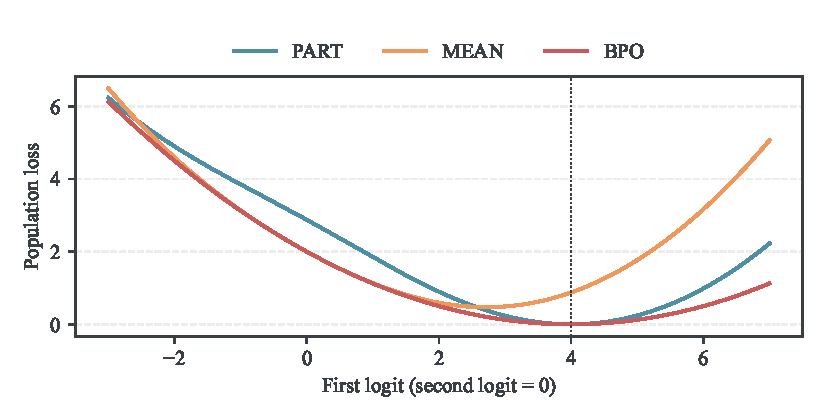
\includegraphics[width=0.96\textwidth]{../../results/book-reconstruction/identities.pdf}
\caption{二元 Categorical 分布下三种同尺度回归目标函数曲线。参数为 $q=(1/2,1/2)$、$f=(2,-2)$、$\eta=1$，第二个 Logit 固定为零；竖直虚线 $z_1=4$ 对应共同 Gibbs 目标。PMD-Part 与 BPO 的总体零损失位置完全相同（但 Part 在 $z_1=0$ 附近呈负曲率），而 PMD-Mean 的最优点严格偏离。}
\label{evidence:identities-figure}
\end{figure}

\section{四动作可枚举内层轨迹与目标差异定量拆解}

实验脚本位于 \path{experiments/toy/toy_token_inner.py}（结果保存于 \path{results/toy/toy_token_inner.csv}）。固定单个四动作前缀：
\begin{equation}
 q_0=(0.62,0.23,0.10,0.05),
 \qquad
 t=(0.08,0.17,0.25,0.50).
\end{equation}
为检验离开锚点后的梯度差异，四个方法从偏离锚点的同一初始策略 $p_{0,0}=(0.70,0.15,0.10,0.05)$ 出发，以学习率 $0.15$ 运行 $N=400$ 步完整词表更新（MDPO 采用精确 Categorical Fisher 预条件器）。记方法 $M$ 的自身总体最优分布为 $p_0^{\star,M}$（PMD-Mean 由 Lambert-$W$ 方程求解，其余三种方法为 $p_0^{\mathrm G}$），定义三项 TV 距离指标：
\begin{align*}
e^{\mathrm{opt}}_M&=\operatorname{TV}(p_{0,N},p_0^{\star,M}),\\
e^{\mathrm{Gibbs}}_M&=\operatorname{TV}(p_{0,N},p_0^{\mathrm G}),\\
e^{\mathrm{target}}_M&=\operatorname{TV}(p_0^{\star,M},p_0^{\mathrm G}).
\end{align*}
其中 $e^{\mathrm{opt}}_M$ 度量有限步数值优化误差，$e^{\mathrm{target}}_M$ 度量方法总体目标与 Gibbs 解的结构性偏差。

\begin{table}[ht]
\centering
\caption{固定测度四 Token 内层的可枚举实验（400 步更新后三项 TV 距离拆解）}
\label{tab:toy-results}
\begin{tabular}{llrrr}
\toprule
$\eta$ & 方法 $M$ & 优化误差 $e^{\mathrm{opt}}_M$ & 到 Gibbs 距离 $e^{\mathrm{Gibbs}}_M$ & 目标结构偏差 $e^{\mathrm{target}}_M$\\
\midrule
0.25 & PMD-Part & 1.11e-03 & 1.11e-03 & 0.00e+00\\
0.25 & PMD-Mean & 6.81e-04 & 9.26e-03 & 9.12e-03\\
0.25 & BPO & 1.96e-08 & 1.96e-08 & 0.00e+00\\
0.25 & MDPO & 8.33e-17 & 8.33e-17 & 0.00e+00\\
0.50 & PMD-Part & 2.65e-03 & 2.65e-03 & 0.00e+00\\
0.50 & PMD-Mean & 3.58e-04 & 6.86e-02 & 6.85e-02\\
0.50 & BPO & 1.23e-04 & 1.23e-04 & 0.00e+00\\
0.50 & MDPO & 1.25e-16 & 1.25e-16 & 0.00e+00\\
0.80 & PMD-Part & 2.97e-03 & 2.97e-03 & 0.00e+00\\
0.80 & PMD-Mean & 4.11e-05 & 1.90e-01 & 1.90e-01\\
0.80 & BPO & 4.53e-03 & 4.53e-03 & 0.00e+00\\
0.80 & MDPO & 2.78e-16 & 2.78e-16 & 0.00e+00\\
\bottomrule
\end{tabular}
\end{table}

如表~\ref{tab:toy-results} 所示，PMD-Mean 到自身最优解的误差 $e^{\mathrm{opt}}_{\mathrm{Mean}}$ 随优化迅速降至 $4.11\times 10^{-5}$（$\eta=0.80$），但到 Gibbs 解的距离 $e^{\mathrm{Gibbs}}_{\mathrm{Mean}}$ 被锁定在结构性差异 $e^{\mathrm{target}}_{\mathrm{Mean}}=0.1904$ 上。BPO 的损失带有 $1/\eta$ 缩放因子，在固定步长与 400 步预算下，$\eta=0.80$ 时余留 $4.53\times 10^{-3}$ 的有限步优化误差；而使用精确 Categorical Fisher 自然梯度的 MDPO 在全部 $\eta$ 下均达到双精度浮点极限（$\sim 10^{-16}$）。

\section{外层硬同步（Hard Sync）的局部三次阶数、边界幂率与噪声底核验}
\label{dyn:sec:hard-sync-experiments}

本节使用程序 \path{experiments/toy/hard_sync_audit.py}（结果保存在 \path{results/hard-sync-audit/}，float64 精度，随机种子 $20261010$）核验第~\ref{dyn:chapter} 章的外层硬同步动力学定理。

\subsection{五项预设可证伪数值判据与高精度级数求值}

实验在运行前固定五项数值判据：
\begin{enumerate}
 \item \textbf{Gibbs 跨度收缩与三点恒等式}：在词表大小 $V\in\{2,4,8\}$（每个大小生成 $12$ 组独立正分布）、步长 $\eta\in\{0.2,0.8,1,1.2,1.8,2,2.2\}$ 共 $252$ 个更新上，绝对残差阈值设为 $10^{-12}$。
 \item \textbf{Mean 求解器一致性}：独立 SciPy Lambert-$W$ 求解器与仓库 \path{token_inner.mean_target} 在 $36$ 组输出上的逐坐标差、KKT 残差与归一化残差阈值均设为 $10^{-12}$（求根器使用 $\E_q\operatorname{expm1}(G-W_0(\lambda e^G))=0$ 避免相近数相减）。
 \item \textbf{Mean 在 $\eta=1$ 的局部三次收敛阶数}：固定 $t=(0.2,0.3,0.5)$、扰动方向 $z=(-1,0.2,0.8)$（此时 $\Var_t(z)=0.4644,\;\operatorname{osc}z=1.8$），令 $q_\epsilon\propto t\exp(\epsilon z)$，扫描 $\epsilon\in\{0.4,0.2,0.1,0.05,0.02,0.01\}$。由于三次收敛极快进入机器精度，程序令 $d_a=p_a/t_a-1$（满足 $\sum_a t_a d_a=0$），将 KL 改写为 $\KL(p\Vert t)=\sum_a t_a\{(1+d_a)\log(1+d_a)-d_a\}$，并在 $|d_a|<10^{-3}$ 时使用高阶级数：
\begin{equation*}
 (1+d)\log(1+d)-d
 =\sum_{n=2}^{9}\frac{(-1)^n d^n}{n(n-1)}+O(d^{10}).
\end{equation*}
由定理~\ref{dyn:thm:mean-hard-sync-local-expansion}，KL 三次比值 $\KL(p^\star\Vert t)/\KL(q_\epsilon\Vert t)^3$ 理论极限为 $1$，跨度三次比值理论极限为
\begin{equation*}
 \lim_{\epsilon\to 0}\frac{b(p^\star,t)}{b(q_\epsilon,t)^3}=
 \frac{\Var_t(z)}{2(\operatorname{osc}z)^2}=\frac{0.4644}{2\cdot1.8^2}=0.071666\ldots.
\end{equation*}
 \item \textbf{临界步长 $\eta=2$ 的 $1/(16k)$ 幂率}：从 $q_0\propto t\exp(0.2z)$ 出发运行 $10{,}000$ 轮 $\eta=2$ 的精确更新，检验 Gibbs 保持二周期而 Mean 的 $k\KL(q_k\Vert t)$ 趋近定理~\ref{dyn:thm:mean-hard-sync-boundary-rate} 的极限 $1/16=0.0625$。
 \item \textbf{输出噪声与奖励噪声的有限时间协方差预测}：生成独立 $\mathcal N(0,\sigma^2 I)$（$\sigma=0.01$）向量并减去教师均值，此时 $\E\|\xi\|_t^2=\sigma^2(1-\sum_a t_a^2)$。按式~\eqref{dyn:eq:hs-centered-linear} 运行 $20{,}000$ 条独立路径、$K=240$ 步（$\eta\in\{0.2,0.5,1,1.5,1.8\}$），与有限时间理论预测值
\begin{equation*}
 \E\|y_K\|_t^2=
 \sigma^2\left(1-\sum_a t_a^2\right)
 \frac{1-(1-\eta)^{2K}}{\eta(2-\eta)}
 \quad\text{（奖励噪声再乘以 }\eta^2\text{）}
\end{equation*}
对照，要求样本均值全部落入预测值的 $5$ 个 Monte Carlo 标准误以内。
\end{enumerate}

表~\ref{dyn:tab:hard-sync-audit} 与图~\ref{dyn:fig:hard-sync-audit} 展示了全部实测结果，五项判据全部精确通过。

\begin{table}[htbp]
 \centering
 \caption{精确硬同步（Hard Sync）更新的数值审计结果}
 \label{dyn:tab:hard-sync-audit}
 \begin{tabular}{ll}
 \toprule
 审计项目 & 实测结果与理论极限\\
 \midrule
 Gibbs 三点恒等式最大绝对残差 & $1.78\times10^{-15}$\\
 Mean 独立求解与参考实现最大坐标差 & $2.78\times10^{-16}$\\
 Mean KKT 与归一化最大残差 & $3.55\times10^{-15}$\\
 $\epsilon=0.01$ 的 KL 三次比值 $\KL^+/(\KL)^3$ & $1.011557$（理论极限为 $1$）\\
 同一点的跨度三次比值 $b^+/b^3$ & $0.071591$（理论极限为 $0.071667$）\\
 $\eta=2$、$k=10{,}000$ 的 Mean $k\KL(q_k\Vert t)$ & $0.062303$（理论极限为 $0.0625$）\\
 \bottomrule
 \end{tabular}
\end{table}

\begin{figure}[htbp]
 \centering
 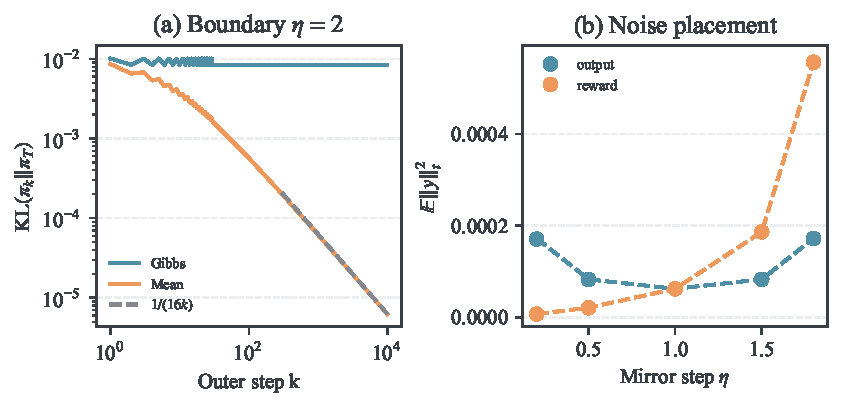
\includegraphics[width=0.96\textwidth]{../../results/hard-sync-audit/hard-sync.pdf}
 \caption{固定三元词表下的硬同步审计。左：$\eta=2$ 下精确 Gibbs 的二周期振荡与 PMD-Mean 的 $1/(16k)$ 幂率衰减；右：固定输出噪声和固定奖励噪声的教师加权二阶矩（点与实线为数值模拟，虚线为独立理论预测）。}
 \label{dyn:fig:hard-sync-audit}
\end{figure}

\section{幂均值中心与 Head--Tail 区间估计的真实模型缓存审计}

脚本 \path{experiments/analysis/power_center_advantage.py} 对原模型缓存的 64 条回复轨迹按每条 2 个固定随机水库抽样位置提取共 128 个真实前缀，在 20 组 $(\kappa,\eta)$ 网格上精确计算全词表条件矩、式~\eqref{eq:center-head-tail-interval} 的确定性区间 $[L,U]$ 以及定理~\ref{thm:center-tail-bounded-estimator} 的区间内无偏尾部估计器条件矩（结果保存于 \path{results/power-center-advantage/} 与 \path{results/power-center-extensions/}）。如图~\ref{fig:cached-head-tail-estimation} 所示，扩大保留头部大小单调收紧统一区间宽度 $w=U-L$ 与最坏方差保证。

\begin{figure}[htbp]
 \centering
 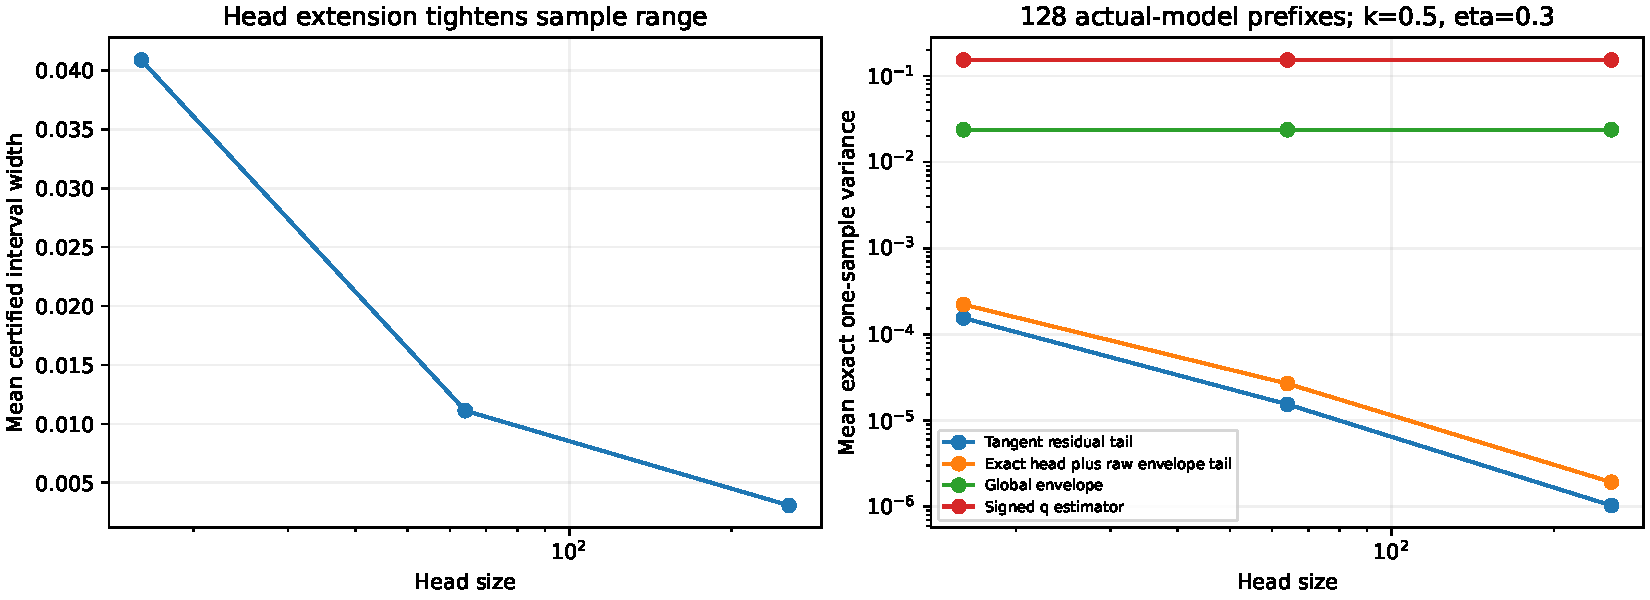
\includegraphics[width=\textwidth]{../../results/power-center-extensions/cached-head-tail-estimation.pdf}
 \caption{原模型缓存 128 个固定前缀上的 Head--Tail 确定性区间与区间内无偏尾部估计器条件矩。}
 \label{fig:cached-head-tail-estimation}
\end{figure}


\chapter{语言模型蒸馏实验、标量调度与 ResOPD 系统评估}
\label{ch:llm-experiments}

本章汇总真实语言模型上的四组系统级实验：Qwen3-1.7B/4B 在 GSM8K 上的 350,166 个前缀 Top-$J$ 估计器对照、Pythia-14M/70M 上的 On-Policy 与 Token-IS 基线记录、DeepSeek-1.5B 在固定监督下的三点方向线搜索与标量调度验证，以及 ResOPD 的代码调用链与推理基准实验。

\section{真实语言模型（Qwen3-1.7B/4B）上的四种 \texorpdfstring{Top-$J$}{Top-J} 估计器对照}

我们使用 GSM8K 测试集的全部 1,319 个提示，以 Qwen3-1.7B 为学生、Qwen3-4B 为教师，采样温度固定为 $1.0$，对每个提示生成一条完整学生轨迹，总计获得 \textbf{350,166 个有效前缀}。打分阶段在 NF4 权重量化、BF16 计算下求出每个前缀的学生与教师完整词表分布，将其完整求和
\begin{equation}
 \mathcal K^{\mathrm{full}}(s)=\KL\bigl(p_{k,n}(\cdot\mid s)\Vert t(\cdot\mid s)\bigr)
\end{equation}
作为该量化模型对的精确真值（Oracle）。生成阶段采用 BF16 vLLM，因此图~\ref{fig:qwen-topk-four} 将按 NF4 学生分布精确计算的 EMA 理论方差曲线与使用 BF16 采样 Token 的 EMA 实测曲线分开报告。Tail-Aware 尾部总质量在 float64 下直接累加尾部概率，避免头部质量接近 $1$ 时用 $1-P_J$ 相减损失有效数字。实验元数据、逐 $J$ 汇总表与绘图脚本分别位于 \path{results/qwen3_gsm8k_pair_kl/metadata.json}、\path{results/qwen3_gsm8k_pair_kl/kl_summary_by_k.csv} 与 \path{experiments/plotting/plot_pair_kl.py}。

\begin{table}[ht]
\centering
\small
\caption{Qwen3-1.7B 学生与 Qwen3-4B 教师在 350,166 个 GSM8K Rollout 前缀上的 Top-$J$ KL 统计（EMA 的 RMSE 是理论单样本尾部校正 RMSE；Normalized 在 $J=0$ 未定义）}
\label{tab:qwen-topk-four}
\begin{tabular}{rrrrrrr}
\toprule
$J$ & $P_J$ & $\mathrm{bias}_{\mathrm{trunc}}$ & $\mathrm{RMSE}_{\mathrm{trunc}}$ & $\mathrm{RMSE}_{\mathrm{EMA}}$ & $\mathrm{bias}_{\mathrm{norm}}$ & $\mathrm{RMSE}_{\mathrm{norm}}$\\
\midrule
0  & 0       & -0.26932 & 1.03968 & 0.80948 & --       & --\\
1  & 0.94208 & -0.07672 & 0.39307 & 0.68557 & -0.26932 & 1.03968\\
2  & 0.98676 & -0.02187 & 0.15337 & 0.40189 & -0.08392 & 0.54660\\
4  & 0.99747 & -0.00465 & 0.04761 & 0.18864 & -0.02629 & 0.28804\\
8  & 0.99949 & -0.00094 & 0.01416 & 0.08308 & -0.00874 & 0.15007\\
16 & 0.99988 & -0.00023 & 0.00488 & 0.03959 & -0.00310 & 0.08367\\
32 & 0.99996 & -0.00008 & 0.00217 & 0.02249 & -0.00127 & 0.05438\\
\bottomrule
\end{tabular}
\end{table}

\begin{table}[ht]
\centering
\caption{同一批 350,166 个 GSM8K 前缀上的 Tail-Aware Top-$J$ 结果（条件采样方差在所有 $J$ 上恒为零）}
\label{tab:qwen-tail-aware}
\begin{tabular}{rrrr}
\toprule
$J$ & 平均 Tail-Aware KL & 条件偏差 $\mathrm{bias}$ & $\mathrm{RMSE}$\\
\midrule
0 & 0 & -0.269321 & 1.039683\\
1 & 0.209759 & -0.059561 & 0.295078\\
2 & 0.248414 & -0.020907 & 0.131407\\
4 & 0.263978 & -0.005343 & 0.045886\\
8 & 0.268091 & -0.001230 & 0.015303\\
16 & 0.269006 & -0.000315 & 0.005493\\
32 & 0.269220 & -0.000101 & 0.002391\\
\bottomrule
\end{tabular}
\end{table}

\begin{figure}[ht]
\centering
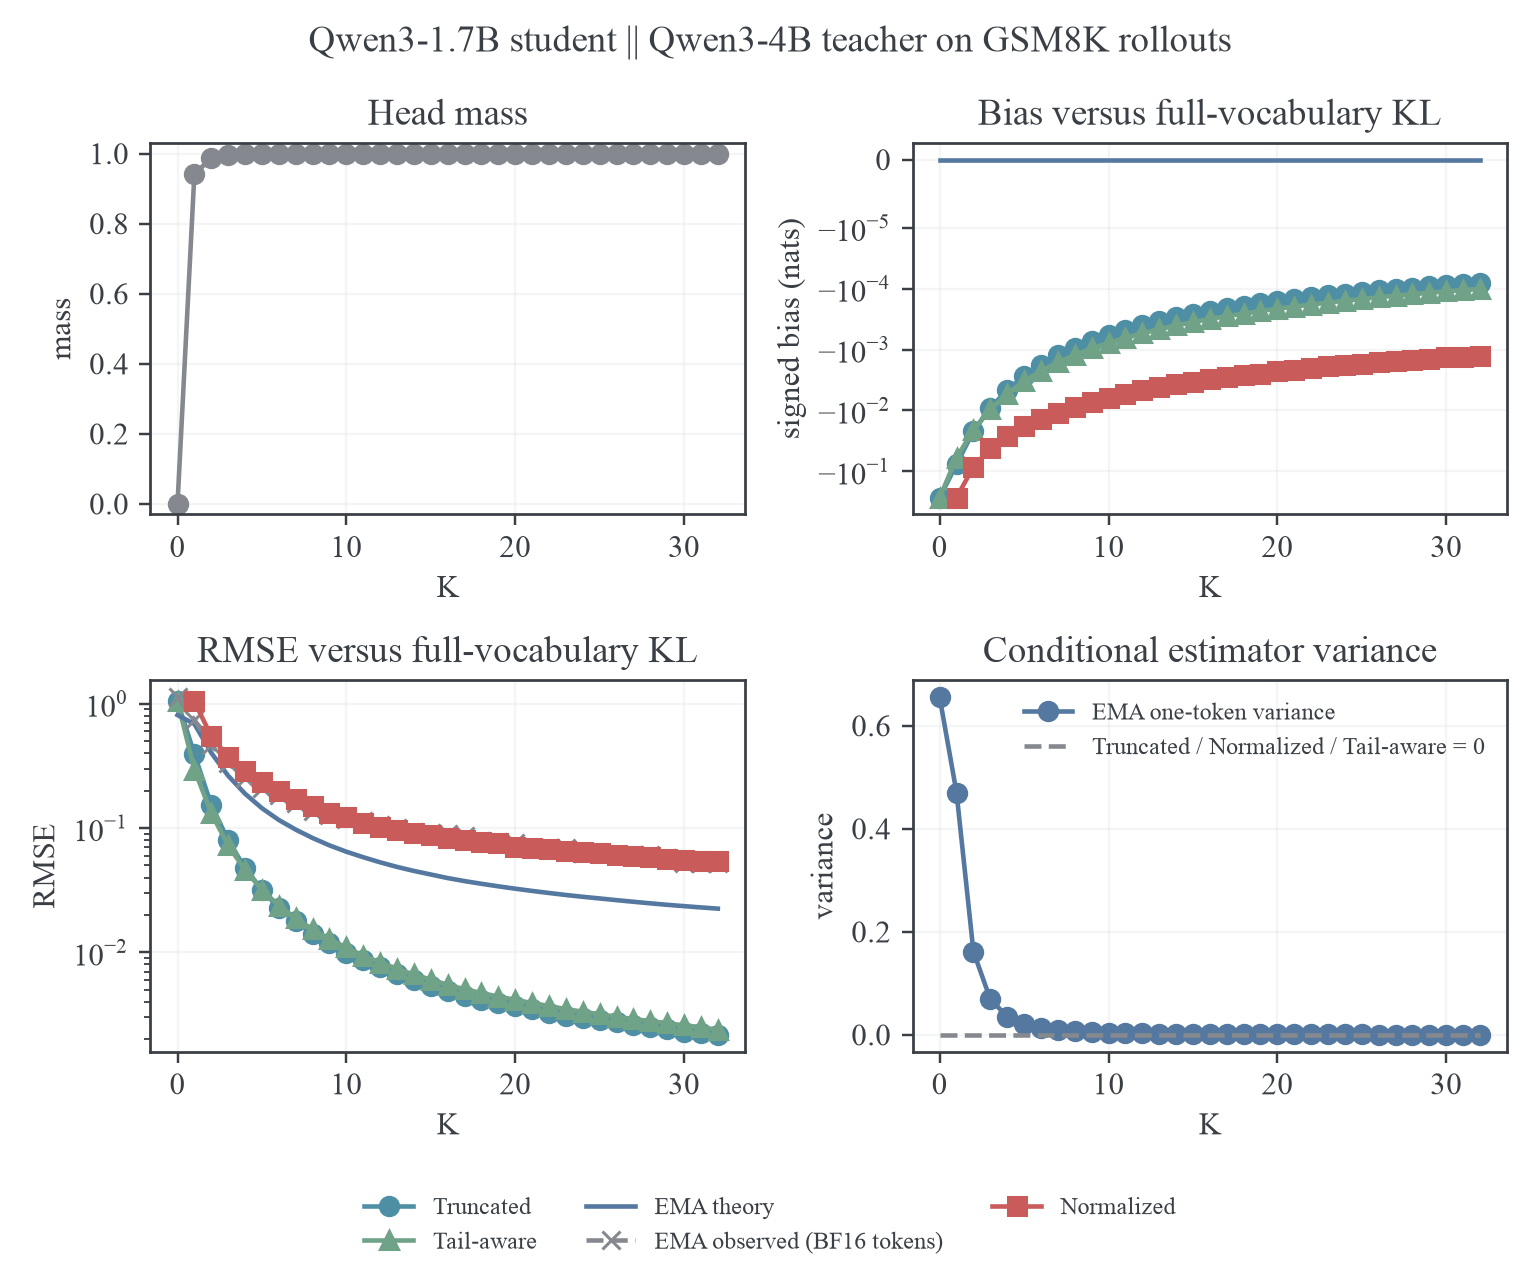
\includegraphics[width=0.96\textwidth]{../../results/qwen3_gsm8k_pair_kl/pair_kl_topk_metrics.png}
\caption{真实 GSM8K Rollout 上四种 Top-$J$ KL 的误差曲线。bias 保留正负号；variance 是固定前缀的条件采样方差而非跨前缀波动。EMA observed 使用 BF16 Rollout Token，与 NF4 打分分布的理论曲线分开展示。}
\label{fig:qwen-topk-four}
\end{figure}

表~\ref{tab:qwen-topk-four} 与表~\ref{tab:qwen-tail-aware} 揭示了四类定义在真实大模型分布上的结构差异：
\begin{enumerate}
\item \textbf{高头部集中度与 EMA 的尾部采样方差代价}：学生 Top-$J$ 质量在 $J=4$ 时已达 $0.99747$，在 $J=32$ 时达 $0.99996$，使确定性截断偏差迅速下降。EMA Top-$J$ 虽在所有 $J$ 上严格无偏，但因尾部对数比率二阶矩较大，在 $J=32$ 时其理论 RMSE 仍为 $0.02249$，高于截断项的 $0.00217$。
\item \textbf{Normalized Top-$J$ 的局部重归一化性质}：$J=1$ 时两侧条件分布均为单点质量，Normalized KL 恒等于零（相对完整 KL 的偏差为 $-0.26932$）；在 $J=32$ 时其 RMSE（$0.05438$）仍远高于截断项与 Tail-Aware，说明它修复的是头部子集上的局部概率归一化，而非完整词表 KL 的高精度估计。
\item \textbf{Tail-Aware 的单调性与正负抵消现象}：Tail-Aware 的 RMSE 随 $J$ 严格单调下降（验证命题~\ref{inf:prop:kl-partition-refinement}）。在 $J=1,2,4$ 时 Tail-Aware 的 RMSE 小于 Truncated；而在 $J=8,16,32$ 时 Truncated 略小，这恰对应第~\ref{est:sec:kl-scalar} 节的分析：Tail-Aware 补回尾部质量项 $M$ 后只剩非正形状偏差 $-B$，而 Truncated 同时丢弃的 $M$ 与 $B$ 在 $M<0$ 时发生了部分正负抵消。
\end{enumerate}

\section{Pythia-14M/70M 基线记录与 DeepSeek-1.5B 标量调度验证}
\label{subsec:ch2-opd-baseline-results}
\label{evidence:scalar}

\subsection{Pythia-14M/70M 基线实验记录}

实验使用 Pythia-14M 学生、Pythia-70M 教师、WikiText 验证集前缀、Top-$J=32$ 锚点支持集、温度 $1.0$、回复长度 $64$、每批 $1024$ 有效 Token、学习率 $10^{-6}$ 和种子 $42$，运行 $32$ 个外层轮次。On-Policy OPD 每轮更新 $N_{\mathrm{inner}}=1$ 次；Token-IS OPD 每轮复用同一批 Rollout 更新 $N_{\mathrm{inner}}=4$ 次。评估在固定的 $8,128$ 个前缀上使用 float32 全词表 Teacher Forcing 精确求和计算：

\begin{center}
\small
\setlength{\tabcolsep}{3pt}
\begin{tabular}{lrrrrrr}
\toprule
方法 & 内层步数 $N_{\mathrm{inner}}$ & 初始 $\KL(p\Vert t)$ & 最终 $\KL(p\Vert t)$ & 初始 $\KL(t\Vert p)$ & 最终 $\KL(t\Vert p)$ & 最终 ESS 比例\\
\midrule
On-Policy OPD & $1$ & 0.9873 & 0.9356 & 0.8907 & 0.8921 & 1.0000\\
Token-IS OPD & $4$ & 0.9873 & 0.9094 & 0.8907 & 0.9387 & 0.9335\\
\bottomrule
\end{tabular}
\end{center}

两种方法均降低了逆向 $\KL(p\Vert t)$。Token-IS 借助每轮 4 次更新将 $\KL(p\Vert t)$ 降得更多（$0.9094$），但正向 $\KL(t\Vert p)$ 上升至 $0.9387$，且有效样本量（ESS）比例降至 $93.35\%$。实验记录中得分系数 RMS 约为 $2.9$--$3.1$，裁剪前梯度范数约为 $1.6\times 10^3$--$2.1\times 10^3$；在分布式 FSDP 训练中需显式固定 \path{mixed_precision} 配置并同时监控 ESS 与全词表固定前缀 KL。

\subsection{固定监督下的标量步长调度验证（DeepSeek-1.5B）}

为验证第~\ref{dyn:scalar} 节的全局标量调度理论，实验涵盖 690 条可控二次轨迹、540 条共享分类模型轨迹（各条件 5 个随机种子）以及 4 张 GPU 上的 \textbf{20 条 DeepSeek-1.5B 固定前缀轨迹}（固定 13 条 DAPO 提示生成的 416 个锚点采样前缀，内层冻结缓存、教师、锚点与 $\eta=0.3$；原始轨迹与图表位于 \path{results/scalar-schedule/}）：
\begin{enumerate}
\item \textbf{完整词表 BPO（FP32）分支}：沿标准 AdamW 方向作三点前向搜索，达到初始目标 $0.1\%$ 阈值仅用 \textbf{117 次}反向传播，而常数学习率网格中最快分支需 \textbf{131 次}（减少 $10.7\%$ 反向传播，但累计前向从 133 次增至 469 次，耗时分别为 $82.3$ 秒与 $43.6$ 秒）。三点搜索从第 117 步至第 500 步稳定保持在该阈值以下（常数网格最早保持至终点的分支为 251 步）。三个连续 50 步窗口的平均对数收缩率从 $0.0612$ 降至 $0.0108$ 再降至 $0.00184$，印证了第~\ref{dyn:scalar} 节的方向能力界：标量搜索更好地匹配当前位置的稳定步幅，但不会消除共享参数网络的慢特征谱。
\item \textbf{生产级 Top-16 加尾部桶、固定单采样动作分支}：默认常数学习率下，120 步后经验平方残差降至初始的 $0.0115\%$，但完整词表 BPO 误差仍为初始的 $62.7\%$（调大常数学习率反而恶化完整误差；经验残差搜索的完整误差终值为 $43.0\%$，与更小常数学习率的 $44.1\%$ 相当）。若保持生产级停止梯度方向不变而用完整词表 BPO 误差决定步长接受，出现 \textbf{36 次拒绝}，证实全局标量无法替代因采样池与粗粒化中心缺失的真实下降方向。
\end{enumerate}

\section{ResOPD 实现链路与大规模推理基准实验}
\label{sec:resopd-implementation}

本节将第~\ref{est:chapter} 章的 ResOPD 控制族对应到公开训练代码（开源仓库 \href{https://github.com/InternLM/ResOPD}{InternLM/ResOPD}，论文 \href{https://arxiv.org/abs/2610.04882}{arXiv:2610.04882}）。

\subsection{代码调用链与停止梯度代理实现}

发布代码中注册的新损失模式为 \path{loss_mode=resopd}。教师路径从 \path{verl/experimental/teacher_loop/teacher_manager.py} 开始，vLLM Rollout（\path{verl/workers/rollout/vllm_rollout/prompt_logprobs.py}）同时返回两组字段：
\begin{itemize}
\item \textbf{头部支持集}：\path{prompt_ids} 与 \path{prompt_logprobs}（教师 Top-$J$）；
\item \textbf{实际采样动作}：\path{sampled_prompt_ids} 与 \path{sampled_prompt_logprobs}（即使落在 Top-$J$ 之外也强制保留）。
\end{itemize}
学生 Logits 经 \path{verl/trainer/distillation/fsdp/losses.py} 对齐后，送入 \path{verl/trainer/distillation/resopd.py} 的 \path{resopd_loss}：
\begin{enumerate}
\item 对完整学生 Logits 做 $\log\operatorname{softmax}$，得到头部 $P(v),\;\ell_v$ 与 $P_S$（教师 Top-$J$ 对数概率在输入时 detach）；
\item 从实际采样 Token 得到 $\ell_A$，并由 \path{student_tail_mass} 与 \path{teacher_tail_mass} 构造 $\ell_{\mathrm{mass}}=\log(\tau_P/\tau_Q)$；
\item 用 \path{support_score} 计算 $b_{\mathrm{TA}}=\ell_{\mathrm{mass}}\nabla_\theta\log\tau_P$，并令 \path{centered_event} 等于 $\mathbf1\{A\in S\}-P_S=\tau_P-J_A$；
\item 通过 \path{surrogate - surrogate.detach()} 保留前向数值、替换反向传播导数，精确实现定理~\ref{est:thm:chapter3-resopd} 中 $b=b_{\mathrm{TA}}$ 的 ResOPD 梯度估计器。
\end{enumerate}

\subsection{公开实验、方差审计与推理基准对比}

论文实验涵盖三组核心对照：（1）有偏确定性 Top-$k$ 方法（Teacher Top-$k$ fKL、Teacher Top-$k$ rKL、TA-OPD）；（2）无偏逆向 KL 梯度估计器（Sampled-Token OPD、教师 Top-$k$ 支持上的 vOPD、HETS、ResOPD）；（3）机制消融（支持集大小 $J\in\{1,4,16,32,64\}$、完整祖先采样 vs. Top-$p$/Top-$k$ 截断、学习率敏感性，以及双控制族中的 SC-TA $\vartheta=1$ vs. ResOPD $\vartheta=0$）。
\begin{itemize}
\item \textbf{冻结前缀全动作方差审计}：在 GSM8K、HMMT26 与 DeepMath 前缀上枚举完整词表动作。在 Top-$4$（$J=4$）下，ResOPD 相对 Sampled-Token OPD \textbf{降低 $52.5\%$--$75.0\%$ 的梯度协方差迹}，并在全部五个评测面板中优于 HETS。
\item \textbf{端到端数学推理与科学/代码迁移}：数学实验使用 Qwen3.5-27B 教师蒸馏 Qwen3.5-4B 学生，在 DeepMath、AIME26、HMMT26、OlymMATH 上 ResOPD 取得 \textbf{$50.12\%$} 平均分，显著优于 HETS 的 \textbf{$45.72\%$}；科学/代码迁移实验使用 Qwen3-30B-A3B-Instruct 蒸馏 Qwen3-4B，在 GPQA-D、SuperGPQA、LiveCodeBench v5/v6 上 ResOPD 取得 \textbf{$44.15\%$} 平均分，优于 HETS 的 \textbf{$43.63\%$}。仓库公开了包含 1,024 条训练样本和 252 条测试样本的 DeepMath 可运行子集（入口 \path{examples/resopd/run_resopd.sh}）及 35 项自动化测试（\path{tests/resopd}）。
\end{itemize}

\backmatter
\chapter*{参考资料与来源说明}
\addcontentsline{toc}{chapter}{参考资料与来源说明}
\begingroup\raggedright
\begin{itemize}
\item \textbf{PMD-Mean 与 Lambert-$W$ 投影理论}：PMD-Mean 的奖励中心化目标与二元奖励分析参考 \href{https://arxiv.org/abs/2602.05933}{arXiv:2602.05933}。本书第~\ref{ch:four-methods} 章与第~\ref{dyn:chapter} 章独立给出了一般多值冻结信号下的受约束全局最优性证明、混合 $\KL$--$\chi^2$ 变分对偶、$\eta\to\infty$ 正部加权极限、硬同步全局稳定区间 $0<\eta\le 2$、$\eta=1$ 的局部三次收敛率以及 $\eta=2$ 的 $1/(16k)$ 边界幂率定理。
\item \textbf{稀疏 Top-$J$ 条件 KL 估计与自动微分算子}：K3$^{++}$、K4、K5 及 EMA Top-$J$ 估计器的公开代码实现源自 \href{https://arxiv.org/abs/2602.04417}{arXiv:2602.04417}（仓库版本 \href{https://github.com/LunjunZhang/ema-pg/blob/f9b977632ad948ce935432a517c22291bfaba562/search/verl/trainer/ppo/core_algos.py}{\path{ema-pg@f9b9776}}）；ResOPD 与双控制族（HETS、ResOPD、SC-TA）源自 \href{https://arxiv.org/abs/2610.04882}{arXiv:2610.04882}（开源仓库 \href{https://github.com/InternLM/ResOPD}{\path{InternLM/ResOPD}}）。本书第~\ref{est:chapter} 章与第~\ref{opd:chapter} 章建立了统一的分区链式分解、Gram 矩阵最优控制、固定样本势函数与非保守旋度理论。
\item \textbf{信息几何、$\alpha$-散度重心与算术混合蒸馏}：概率单纯形上的对偶平坦几何与 $\alpha$-散度重心参考 Shun-ichi Amari (Neural Computation, 2007; ETVC, 2009) 及 Itoh \& Satoh (\href{https://arxiv.org/html/2208.11861}{arXiv:2208.11861})；算术混合教师组件参考 Trust Region Policy Distillation (\href{https://arxiv.org/html/2607.04751v1}{arXiv:2607.04751})。本书第~\ref{ch:proximal-families} 章与第~\ref{est:chapter} 章独立构建了逆向积分精确 MD 教师目标 $\mathcal J_{\kappa,\eta}$、$\kappa\le 1/2$ 二阶矩形状阈值、平方根形状相对误差噪声最优性、有界包络中心提案 $\mu_c$、Head--Tail 区间内无偏估计器以及无重复动作抽样的半正定协方差改进定理。
\end{itemize}
\par\endgroup
\end{document}
